\documentclass[]{book}
\usepackage{lmodern}
\usepackage{amssymb,amsmath}
\usepackage{ifxetex,ifluatex}
\usepackage{fixltx2e} % provides \textsubscript
\ifnum 0\ifxetex 1\fi\ifluatex 1\fi=0 % if pdftex
  \usepackage[T1]{fontenc}
  \usepackage[utf8]{inputenc}
\else % if luatex or xelatex
  \ifxetex
    \usepackage{mathspec}
  \else
    \usepackage{fontspec}
  \fi
  \defaultfontfeatures{Ligatures=TeX,Scale=MatchLowercase}
\fi
% use upquote if available, for straight quotes in verbatim environments
\IfFileExists{upquote.sty}{\usepackage{upquote}}{}
% use microtype if available
\IfFileExists{microtype.sty}{%
\usepackage{microtype}
\UseMicrotypeSet[protrusion]{basicmath} % disable protrusion for tt fonts
}{}
\usepackage[margin=1in]{geometry}
\usepackage{hyperref}
\hypersetup{unicode=true,
            pdftitle={Quantitive Social Science: The R Tidyverse Code},
            pdfauthor={Jeffrey B. Arnold},
            pdfborder={0 0 0},
            breaklinks=true}
\urlstyle{same}  % don't use monospace font for urls
\usepackage{color}
\usepackage{fancyvrb}
\newcommand{\VerbBar}{|}
\newcommand{\VERB}{\Verb[commandchars=\\\{\}]}
\DefineVerbatimEnvironment{Highlighting}{Verbatim}{commandchars=\\\{\}}
% Add ',fontsize=\small' for more characters per line
\usepackage{framed}
\definecolor{shadecolor}{RGB}{248,248,248}
\newenvironment{Shaded}{\begin{snugshade}}{\end{snugshade}}
\newcommand{\AlertTok}[1]{\textcolor[rgb]{0.94,0.16,0.16}{#1}}
\newcommand{\AnnotationTok}[1]{\textcolor[rgb]{0.56,0.35,0.01}{\textbf{\textit{#1}}}}
\newcommand{\AttributeTok}[1]{\textcolor[rgb]{0.77,0.63,0.00}{#1}}
\newcommand{\BaseNTok}[1]{\textcolor[rgb]{0.00,0.00,0.81}{#1}}
\newcommand{\BuiltInTok}[1]{#1}
\newcommand{\CharTok}[1]{\textcolor[rgb]{0.31,0.60,0.02}{#1}}
\newcommand{\CommentTok}[1]{\textcolor[rgb]{0.56,0.35,0.01}{\textit{#1}}}
\newcommand{\CommentVarTok}[1]{\textcolor[rgb]{0.56,0.35,0.01}{\textbf{\textit{#1}}}}
\newcommand{\ConstantTok}[1]{\textcolor[rgb]{0.00,0.00,0.00}{#1}}
\newcommand{\ControlFlowTok}[1]{\textcolor[rgb]{0.13,0.29,0.53}{\textbf{#1}}}
\newcommand{\DataTypeTok}[1]{\textcolor[rgb]{0.13,0.29,0.53}{#1}}
\newcommand{\DecValTok}[1]{\textcolor[rgb]{0.00,0.00,0.81}{#1}}
\newcommand{\DocumentationTok}[1]{\textcolor[rgb]{0.56,0.35,0.01}{\textbf{\textit{#1}}}}
\newcommand{\ErrorTok}[1]{\textcolor[rgb]{0.64,0.00,0.00}{\textbf{#1}}}
\newcommand{\ExtensionTok}[1]{#1}
\newcommand{\FloatTok}[1]{\textcolor[rgb]{0.00,0.00,0.81}{#1}}
\newcommand{\FunctionTok}[1]{\textcolor[rgb]{0.00,0.00,0.00}{#1}}
\newcommand{\ImportTok}[1]{#1}
\newcommand{\InformationTok}[1]{\textcolor[rgb]{0.56,0.35,0.01}{\textbf{\textit{#1}}}}
\newcommand{\KeywordTok}[1]{\textcolor[rgb]{0.13,0.29,0.53}{\textbf{#1}}}
\newcommand{\NormalTok}[1]{#1}
\newcommand{\OperatorTok}[1]{\textcolor[rgb]{0.81,0.36,0.00}{\textbf{#1}}}
\newcommand{\OtherTok}[1]{\textcolor[rgb]{0.56,0.35,0.01}{#1}}
\newcommand{\PreprocessorTok}[1]{\textcolor[rgb]{0.56,0.35,0.01}{\textit{#1}}}
\newcommand{\RegionMarkerTok}[1]{#1}
\newcommand{\SpecialCharTok}[1]{\textcolor[rgb]{0.00,0.00,0.00}{#1}}
\newcommand{\SpecialStringTok}[1]{\textcolor[rgb]{0.31,0.60,0.02}{#1}}
\newcommand{\StringTok}[1]{\textcolor[rgb]{0.31,0.60,0.02}{#1}}
\newcommand{\VariableTok}[1]{\textcolor[rgb]{0.00,0.00,0.00}{#1}}
\newcommand{\VerbatimStringTok}[1]{\textcolor[rgb]{0.31,0.60,0.02}{#1}}
\newcommand{\WarningTok}[1]{\textcolor[rgb]{0.56,0.35,0.01}{\textbf{\textit{#1}}}}
\usepackage{longtable,booktabs}
\usepackage{graphicx,grffile}
\makeatletter
\def\maxwidth{\ifdim\Gin@nat@width>\linewidth\linewidth\else\Gin@nat@width\fi}
\def\maxheight{\ifdim\Gin@nat@height>\textheight\textheight\else\Gin@nat@height\fi}
\makeatother
% Scale images if necessary, so that they will not overflow the page
% margins by default, and it is still possible to overwrite the defaults
% using explicit options in \includegraphics[width, height, ...]{}
\setkeys{Gin}{width=\maxwidth,height=\maxheight,keepaspectratio}
\IfFileExists{parskip.sty}{%
\usepackage{parskip}
}{% else
\setlength{\parindent}{0pt}
\setlength{\parskip}{6pt plus 2pt minus 1pt}
}
\setlength{\emergencystretch}{3em}  % prevent overfull lines
\providecommand{\tightlist}{%
  \setlength{\itemsep}{0pt}\setlength{\parskip}{0pt}}
\setcounter{secnumdepth}{5}
% Redefines (sub)paragraphs to behave more like sections
\ifx\paragraph\undefined\else
\let\oldparagraph\paragraph
\renewcommand{\paragraph}[1]{\oldparagraph{#1}\mbox{}}
\fi
\ifx\subparagraph\undefined\else
\let\oldsubparagraph\subparagraph
\renewcommand{\subparagraph}[1]{\oldsubparagraph{#1}\mbox{}}
\fi

%%% Use protect on footnotes to avoid problems with footnotes in titles
\let\rmarkdownfootnote\footnote%
\def\footnote{\protect\rmarkdownfootnote}

%%% Change title format to be more compact
\usepackage{titling}

% Create subtitle command for use in maketitle
\newcommand{\subtitle}[1]{
  \posttitle{
    \begin{center}\large#1\end{center}
    }
}

\setlength{\droptitle}{-2em}
  \title{Quantitive Social Science: The R Tidyverse Code}
  \pretitle{\vspace{\droptitle}\centering\huge}
  \posttitle{\par}
  \author{Jeffrey B. Arnold}
  \preauthor{\centering\large\emph}
  \postauthor{\par}
  \predate{\centering\large\emph}
  \postdate{\par}
  \date{2018-02-26}


\usepackage{amsthm}
\newtheorem{theorem}{Theorem}[chapter]
\newtheorem{lemma}{Lemma}[chapter]
\theoremstyle{definition}
\newtheorem{definition}{Definition}[chapter]
\newtheorem{corollary}{Corollary}[chapter]
\newtheorem{proposition}{Proposition}[chapter]
\theoremstyle{definition}
\newtheorem{example}{Example}[chapter]
\theoremstyle{definition}
\newtheorem{exercise}{Exercise}[chapter]
\theoremstyle{remark}
\newtheorem*{remark}{Remark}
\newtheorem*{solution}{Solution}
\begin{document}
\maketitle

{
\setcounter{tocdepth}{1}
\tableofcontents
}
\hypertarget{preface}{%
\chapter*{Preface}\label{preface}}
\addcontentsline{toc}{chapter}{Preface}

This is tidyverse R code to supplement the book,
\href{http://press.princeton.edu/titles/11025.html}{Quantitative Social
Science: An Introduction}, by Kosuke Imai.

The R code included with the text of \emph{QSS} and the supplementary
materials relies mostly on base R functions. This translates the code
examples provided with \emph{QSS} to tidyverse R code.
\href{https://github.com/tidyverse/tidyverse}{Tidyverse} refers to a set
of packages (\textbf{ggplot2}, \textbf{dplyr}, \textbf{tidyr},
\textbf{readr}, \textbf{purrr}, \textbf{tibble}, and a few others) that
share common data representations, especially the use of data frames for
return values.

This is not a complete introduction to R and the tidyverse. I suggest
pairing it with \href{http://r4ds.had.co.nz/}{R for Data Science} by
Hadley Wickham and Garrett Grolemond.

These materials are supplement to replace the existing \emph{QSS} code
with the tidvyerse dialect of R. Thus it does not replicate the
substantive material, and not meant to be used independently of the
\emph{QSS} text. However, the provided code is not merely a translation
of the \emph{QSS} code. It often uses the topics in \emph{QSS} to delve
deeper into data science, data visualization, and computational topics.

I wrote this code while teaching course that employed both texts in
order to make the excellent examples and statistical material in
\emph{QSS} more compatible with the modern data science using R approach
in \emph{R4DS}.

\hypertarget{colophon}{%
\section*{Colophon}\label{colophon}}
\addcontentsline{toc}{section}{Colophon}

To install the R packages used in this work run the following code,
installs the \textbf{qsstidy} package which contains no code or data,
but will install the needed dependencies.

\begin{Shaded}
\begin{Highlighting}[]
\KeywordTok{install.packages}\NormalTok{(}\StringTok{"devtools"}\NormalTok{)}
\KeywordTok{install_github}\NormalTok{(}\StringTok{"jrnold/qss-tidy"}\NormalTok{)}
\end{Highlighting}
\end{Shaded}

Additionally, the
\href{https://cran.r-project.org/package=gganimate}{gganimate} package
requires installing \href{https://ffmpeg.org/}{ffmpeg} with libvpx
support.

The source of the book is available
\href{https://github.com/jrnold/qsstidy}{here} and was built with
versions of packages below:

\begin{verbatim}
#> Session info -------------------------------------------------------------
#>  setting  value                       
#>  version  R version 3.4.3 (2017-11-30)
#>  system   x86_64, darwin15.6.0        
#>  ui       X11                         
#>  language (EN)                        
#>  collate  en_US.UTF-8                 
#>  tz       America/Los_Angeles         
#>  date     2017-12-22
#> Packages -----------------------------------------------------------------
#>  package    * version date       source        
#>  animation  * 2.5     2017-03-30 cran (@2.5)   
#>  assertthat   0.2.0   2017-04-11 CRAN (R 3.4.0)
#>  backports    1.1.2   2017-12-13 CRAN (R 3.4.3)
#>  base       * 3.4.3   2017-12-07 local         
#>  bindr        0.1     2016-11-13 CRAN (R 3.4.0)
#>  bindrcpp     0.2     2017-06-17 CRAN (R 3.4.0)
#>  bookdown     0.5     2017-08-20 CRAN (R 3.4.1)
#>  broom        0.4.3   2017-11-20 CRAN (R 3.4.3)
#>  cellranger   1.1.0   2016-07-27 CRAN (R 3.4.0)
#>  cli          1.0.0   2017-11-05 cran (@1.0.0) 
#>  colorspace   1.3-2   2016-12-14 CRAN (R 3.4.0)
#>  compiler     3.4.3   2017-12-07 local         
#>  crayon       1.3.4   2017-09-16 CRAN (R 3.4.1)
#>  datasets   * 3.4.3   2017-12-07 local         
#>  devtools     1.13.4  2017-11-09 CRAN (R 3.4.2)
#>  digest       0.6.13  2017-12-14 CRAN (R 3.4.3)
#>  dplyr      * 0.7.4   2017-09-28 CRAN (R 3.4.2)
#>  evaluate     0.10.1  2017-06-24 CRAN (R 3.4.1)
#>  forcats    * 0.2.0   2017-01-23 CRAN (R 3.4.0)
#>  foreign      0.8-69  2017-06-22 CRAN (R 3.4.3)
#>  ggplot2    * 2.2.1   2016-12-30 CRAN (R 3.4.0)
#>  glue         1.2.0   2017-10-29 CRAN (R 3.4.2)
#>  graphics   * 3.4.3   2017-12-07 local         
#>  grDevices  * 3.4.3   2017-12-07 local         
#>  grid         3.4.3   2017-12-07 local         
#>  gtable       0.2.0   2016-02-26 CRAN (R 3.4.0)
#>  haven        1.1.0   2017-07-09 CRAN (R 3.4.1)
#>  hms          0.4.0   2017-11-23 CRAN (R 3.4.3)
#>  htmltools    0.3.6   2017-04-28 CRAN (R 3.4.0)
#>  httr         1.3.1   2017-08-20 CRAN (R 3.4.1)
#>  jsonlite     1.5     2017-06-01 CRAN (R 3.4.0)
#>  knitr        1.17    2017-08-10 CRAN (R 3.4.1)
#>  lattice      0.20-35 2017-03-25 CRAN (R 3.4.3)
#>  lazyeval     0.2.1   2017-10-29 CRAN (R 3.4.2)
#>  lubridate    1.7.1   2017-11-03 cran (@1.7.1) 
#>  magrittr     1.5     2014-11-22 CRAN (R 3.4.0)
#>  memoise      1.1.0   2017-04-21 CRAN (R 3.4.0)
#>  methods      3.4.3   2017-12-07 local         
#>  mnormt       1.5-5   2016-10-15 CRAN (R 3.4.0)
#>  modelr       0.1.1   2017-07-24 CRAN (R 3.4.1)
#>  munsell      0.4.3   2016-02-13 CRAN (R 3.4.0)
#>  nlme         3.1-131 2017-02-06 CRAN (R 3.4.3)
#>  parallel     3.4.3   2017-12-07 local         
#>  pkgconfig    2.0.1   2017-03-21 CRAN (R 3.4.0)
#>  plyr         1.8.4   2016-06-08 CRAN (R 3.4.0)
#>  psych        1.7.8   2017-09-09 CRAN (R 3.4.1)
#>  purrr      * 0.2.4   2017-10-18 cran (@0.2.4) 
#>  R6           2.2.2   2017-06-17 CRAN (R 3.4.0)
#>  Rcpp         0.12.14 2017-11-23 CRAN (R 3.4.3)
#>  readr      * 1.1.1   2017-05-16 CRAN (R 3.4.0)
#>  readxl       1.0.0   2017-04-18 CRAN (R 3.4.0)
#>  reshape2     1.4.3   2017-12-11 CRAN (R 3.4.3)
#>  rlang        0.1.4   2017-11-05 CRAN (R 3.4.2)
#>  rmarkdown    1.8     2017-11-17 CRAN (R 3.4.2)
#>  rprojroot    1.3-1   2017-12-18 CRAN (R 3.4.3)
#>  rstudioapi   0.7     2017-09-07 CRAN (R 3.4.1)
#>  rvest        0.3.2   2016-06-17 CRAN (R 3.4.0)
#>  scales       0.5.0   2017-08-24 CRAN (R 3.4.1)
#>  stats      * 3.4.3   2017-12-07 local         
#>  stringi      1.1.6   2017-11-17 CRAN (R 3.4.2)
#>  stringr    * 1.2.0   2017-02-18 CRAN (R 3.4.0)
#>  tibble     * 1.3.4   2017-08-22 CRAN (R 3.4.1)
#>  tidyr      * 0.7.2   2017-10-16 cran (@0.7.2) 
#>  tidyverse  * 1.2.1   2017-11-14 CRAN (R 3.4.2)
#>  tools        3.4.3   2017-12-07 local         
#>  utils      * 3.4.3   2017-12-07 local         
#>  withr        2.1.1   2017-12-19 cran (@2.1.1) 
#>  xml2         1.1.1   2017-01-24 CRAN (R 3.4.0)
#>  yaml         2.1.16  2017-12-12 CRAN (R 3.4.3)
\end{verbatim}

\hypertarget{introduction}{%
\chapter{Introduction}\label{introduction}}

\hypertarget{prerequisites}{%
\section*{Prerequisites}\label{prerequisites}}
\addcontentsline{toc}{section}{Prerequisites}

In this and other chapters we will make use of data from the
\texttt{qss} package, which is available on github. Install it using the
\texttt{install\_github()} function from the library \texttt{devtools}.

\begin{Shaded}
\begin{Highlighting}[]
\NormalTok{devtools}\OperatorTok{::}\KeywordTok{install_github}\NormalTok{(}\StringTok{"kosukeimai/qss-package"}\NormalTok{)}
\end{Highlighting}
\end{Shaded}

\begin{Shaded}
\begin{Highlighting}[]
\KeywordTok{library}\NormalTok{(}\StringTok{"qss"}\NormalTok{)}
\end{Highlighting}
\end{Shaded}

In the prerequisites section of each chapter, we'll load any packages
needed for the chapter, possibly define some functions, and possibly
load data. It is good practice to load necessary libraries at the start
of an R markdown file or script.

\begin{Shaded}
\begin{Highlighting}[]
\KeywordTok{library}\NormalTok{(}\StringTok{"tidyverse"}\NormalTok{)}
\end{Highlighting}
\end{Shaded}

We also load the \textbf{readr} package to load \texttt{csv} files,

\begin{Shaded}
\begin{Highlighting}[]
\KeywordTok{library}\NormalTok{(}\StringTok{"readr"}\NormalTok{)}
\end{Highlighting}
\end{Shaded}

the \textbf{haven} package to load Stata \texttt{dta} files,

\begin{Shaded}
\begin{Highlighting}[]
\KeywordTok{library}\NormalTok{(}\StringTok{"haven"}\NormalTok{)}
\end{Highlighting}
\end{Shaded}

and the \textbf{rio} package to load multiple types of files

\begin{Shaded}
\begin{Highlighting}[]
\KeywordTok{library}\NormalTok{(}\StringTok{"rio"}\NormalTok{)}
\end{Highlighting}
\end{Shaded}

\hypertarget{overview-of-the-book}{%
\section{Overview of the Book}\label{overview-of-the-book}}

\emph{This sections contains no code to translate -- see}QSS* text.*

\hypertarget{how-to-use-the-book}{%
\section{How to use the Book}\label{how-to-use-the-book}}

\emph{This sections contains no code to translate -- see}QSS* text.*

\hypertarget{introduction-to-r}{%
\section{Introduction to R}\label{introduction-to-r}}

These notes do not aim to completely teach R and the tidyverse. However,
there are many other resources for that.

\href{http://r4ds.had.co.nz/}{R for Data Science} is a comprehensive
introduction to R using the tidyverse.

\href{https://www.datacamp.com/home}{Data Camp} has interactive courses.
In particular, I recommend starting with the following two courses.

\begin{itemize}
\tightlist
\item
  \href{https://www.datacamp.com/courses/free-introduction-to-r}{Introduction
  to R}
\item
  \href{https://www.datacamp.com/courses/introduction-to-the-tidyverse}{Introduction
  to the Tidyverse}
\end{itemize}

\hypertarget{arithmetic-operations}{%
\subsection{Arithmetic Operations}\label{arithmetic-operations}}

This sections contains no code to translate---see \emph{QSS} text.

\hypertarget{objects}{%
\subsection{Objects}\label{objects}}

This sections contains no code to translate---see \emph{QSS} text.

Also see \href{http://r4ds.had.co.nz/workflow-basics.html}{R4DS:
Workflow basics}.

\hypertarget{vectors}{%
\subsection{Vectors}\label{vectors}}

This sections contains no code to translate---see \emph{QSS} text.

Also see \href{http://r4ds.had.co.nz/vectors.html}{R4DS: Vectors}. In
\emph{R for Data Science} vectors are introduced much later, after data
frames.

\hypertarget{functions}{%
\subsection{Functions}\label{functions}}

This sections contains no code to translate---see \emph{QSS} text.

Also see \href{http://r4ds.had.co.nz/functions.html}{R4DS: Functions}.

\hypertarget{data-files}{%
\subsection{Data Files}\label{data-files}}

Rather than using \texttt{setwd()} in scripts, data analysis should be
organized in projects. Read the introduction on RStudio projects in
\href{http://r4ds.had.co.nz/workflow-projects.html}{R4DS}.\footnote{For
  more on using projects read
  \href{https://www.tidyverse.org/articles/2017/12/workflow-vs-script/}{Project-oriented
  workflow}.}

Datasets used in R are accessed in two ways.

\begin{itemize}
\tightlist
\item
  Datasets can be distributed with R packages. These are often smaller
  datasets used in examples and tutorials in packages. These are loaded
  with the \texttt{data()} function. For example you can load UN data on
  demographic statistics from the \textbf{qss} library, which
  distributes the data sets used in the \emph{QSS} textbook. (The
  function \texttt{data()} called without any arguments will list all
  the datasets distributed with installed packages.)
\end{itemize}

\begin{Shaded}
\begin{Highlighting}[]
\KeywordTok{data}\NormalTok{(}\StringTok{"UNpop"}\NormalTok{, }\DataTypeTok{package =} \StringTok{"qss"}\NormalTok{)}
\end{Highlighting}
\end{Shaded}

\begin{itemize}
\tightlist
\item
  Datasets can be loaded from external files including both stored R
  objects (\texttt{.RData}, \texttt{.rda}) and other formats
  (\texttt{.csv}, \texttt{.dta}, \texttt{.sav}). To read a
  \href{https://en.wikipedia.org/wiki/Comma-separated_values}{csv} file
  into R use the \texttt{read\_csv} function from the \textbf{readr}
  library, part of the tidyverse.
\end{itemize}

\begin{Shaded}
\begin{Highlighting}[]
\NormalTok{UNpop_URL <-}\StringTok{ "https://raw.githubusercontent.com/kosukeimai/qss/master/INTRO/UNpop.csv"}
\NormalTok{UNpop <-}\StringTok{ }\KeywordTok{read_csv}\NormalTok{(UNpop_URL)}
\CommentTok{#> Parsed with column specification:}
\CommentTok{#> cols(}
\CommentTok{#>   year = col_integer(),}
\CommentTok{#>   world.pop = col_integer()}
\CommentTok{#> )}
\end{Highlighting}
\end{Shaded}

We use the readr function\texttt{read\_csv()} instead of the base R
function \texttt{read.csv()} used in the \emph{QSS} text. It is slightly
faster, and returns a \texttt{tibble} instead of a data frame. Check
this by calling \texttt{class()} on the new object.

\begin{Shaded}
\begin{Highlighting}[]
\KeywordTok{class}\NormalTok{(UNpop)}
\CommentTok{#> [1] "tbl_df"     "tbl"        "data.frame"}
\NormalTok{UNpop}
\CommentTok{#> # A tibble: 7 x 2}
\CommentTok{#>    year world.pop}
\CommentTok{#>   <int>     <int>}
\CommentTok{#> 1  1950   2525779}
\CommentTok{#> 2  1960   3026003}
\CommentTok{#> 3  1970   3691173}
\CommentTok{#> 4  1980   4449049}
\CommentTok{#> 5  1990   5320817}
\CommentTok{#> 6  2000   6127700}
\CommentTok{#> # ... with 1 more row}
\end{Highlighting}
\end{Shaded}

See \href{http://r4ds.had.co.nz/}{R for Data Science}
\href{http://r4ds.had.co.nz/tibbles.html\#introduction-4}{Ch 11: Data
Import} for more discussion.

Note that in the previous code we loaded the file directly from a URL,
but we could also work with local files on your computer, e.g.

\begin{Shaded}
\begin{Highlighting}[]
\NormalTok{UNpop <-}\StringTok{ }\KeywordTok{read_csv}\NormalTok{(}\StringTok{"INTRO/UNpop.csv"}\NormalTok{)}
\end{Highlighting}
\end{Shaded}

See \href{http://r4ds.had.co.nz/}{R for Data Science}
\href{http://r4ds.had.co.nz/tibbles.html}{Ch 10: Tibbles} for a deeper
discussion of data frames.

The single bracket, \texttt{{[}}, is useful to select rows and columns
in simple cases.

\begin{Shaded}
\begin{Highlighting}[]
\NormalTok{UNpop[}\KeywordTok{c}\NormalTok{(}\DecValTok{1}\NormalTok{, }\DecValTok{2}\NormalTok{, }\DecValTok{3}\NormalTok{), ]}
\CommentTok{#> # A tibble: 3 x 2}
\CommentTok{#>    year world.pop}
\CommentTok{#>   <int>     <int>}
\CommentTok{#> 1  1950   2525779}
\CommentTok{#> 2  1960   3026003}
\CommentTok{#> 3  1970   3691173}
\end{Highlighting}
\end{Shaded}

There are \textbf{dplyr} functions to select rows by number, to select
rows by certain criteria, or to select columns.

To select rows 1--3, use \texttt{slice()}.

\begin{Shaded}
\begin{Highlighting}[]
\KeywordTok{slice}\NormalTok{(UNpop, }\DecValTok{1}\OperatorTok{:}\DecValTok{3}\NormalTok{)}
\CommentTok{#> # A tibble: 3 x 2}
\CommentTok{#>    year world.pop}
\CommentTok{#>   <int>     <int>}
\CommentTok{#> 1  1950   2525779}
\CommentTok{#> 2  1960   3026003}
\CommentTok{#> 3  1970   3691173}
\end{Highlighting}
\end{Shaded}

Base R allows you to choose the column \texttt{world.pop} column from
the \texttt{UNpop} data frame:

\begin{Shaded}
\begin{Highlighting}[]
\NormalTok{UNpop[, }\StringTok{"world.pop"}\NormalTok{]}
\CommentTok{#> # A tibble: 7 x 1}
\CommentTok{#>   world.pop}
\CommentTok{#>       <int>}
\CommentTok{#> 1   2525779}
\CommentTok{#> 2   3026003}
\CommentTok{#> 3   3691173}
\CommentTok{#> 4   4449049}
\CommentTok{#> 5   5320817}
\CommentTok{#> 6   6127700}
\CommentTok{#> # ... with 1 more row}
\NormalTok{UNpop}\OperatorTok{$}\NormalTok{world.pop}
\CommentTok{#> [1] 2525779 3026003 3691173 4449049 5320817 6127700 6916183}
\NormalTok{UNpop[[}\StringTok{"world.pop"}\NormalTok{]]}
\CommentTok{#> [1] 2525779 3026003 3691173 4449049 5320817 6127700 6916183}
\KeywordTok{select}\NormalTok{(UNpop, world.pop)}
\CommentTok{#> # A tibble: 7 x 1}
\CommentTok{#>   world.pop}
\CommentTok{#>       <int>}
\CommentTok{#> 1   2525779}
\CommentTok{#> 2   3026003}
\CommentTok{#> 3   3691173}
\CommentTok{#> 4   4449049}
\CommentTok{#> 5   5320817}
\CommentTok{#> 6   6127700}
\CommentTok{#> # ... with 1 more row}
\end{Highlighting}
\end{Shaded}

Unlike \texttt{{[}}, the \texttt{{[}{[}} and \texttt{\$} operators can
only select a single column and return a vector.\footnote{See the
  discussion in
  \href{http://r4ds.had.co.nz/tibbles.html\#tibbles-vs.data.frame}{R for
  Data Science} on how \texttt{tibble} objects differ from base
  \texttt{data.frame} objects in how \texttt{{[}} is handled.} The
\texttt{dplyr} function \texttt{select()} \textbf{always} returns a
tibble (data frame), and never a vector, even if only one column is
selected.

Select rows 1--3 of the \texttt{year} column:

\begin{Shaded}
\begin{Highlighting}[]
\NormalTok{UNpop[}\DecValTok{1}\OperatorTok{:}\DecValTok{3}\NormalTok{, }\StringTok{"year"}\NormalTok{]}
\CommentTok{#> # A tibble: 3 x 1}
\CommentTok{#>    year}
\CommentTok{#>   <int>}
\CommentTok{#> 1  1950}
\CommentTok{#> 2  1960}
\CommentTok{#> 3  1970}
\end{Highlighting}
\end{Shaded}

or,

\begin{Shaded}
\begin{Highlighting}[]
\KeywordTok{select}\NormalTok{(}\KeywordTok{slice}\NormalTok{(UNpop, }\DecValTok{1}\OperatorTok{:}\DecValTok{3}\NormalTok{), year)}
\CommentTok{#> # A tibble: 3 x 1}
\CommentTok{#>    year}
\CommentTok{#>   <int>}
\CommentTok{#> 1  1950}
\CommentTok{#> 2  1960}
\CommentTok{#> 3  1970}
\end{Highlighting}
\end{Shaded}

The same series of functions can be performed using the pipe operator,
\texttt{\%\textgreater{}\%}.

\begin{Shaded}
\begin{Highlighting}[]
\NormalTok{UNpop }\OperatorTok
\StringTok{  }\KeywordTok{slice}\NormalTok{(}\DecValTok{1}\OperatorTok{:}\DecValTok{3}\NormalTok{) }\OperatorTok
\StringTok{  }\KeywordTok{select}\NormalTok{(year)}
\CommentTok{#> # A tibble: 3 x 1}
\CommentTok{#>    year}
\CommentTok{#>   <int>}
\CommentTok{#> 1  1950}
\CommentTok{#> 2  1960}
\CommentTok{#> 3  1970}
\end{Highlighting}
\end{Shaded}

This example may seem verbose, but later we can produce more complicated
transformations of the data by chaining together simple functions.

Select every other row from \texttt{UNpop}:

\begin{Shaded}
\begin{Highlighting}[]
\NormalTok{UNpop}\OperatorTok{$}\NormalTok{world.pop[}\KeywordTok{seq}\NormalTok{(}\DataTypeTok{from =} \DecValTok{1}\NormalTok{, }\DataTypeTok{to =} \KeywordTok{nrow}\NormalTok{(UNpop), }\DataTypeTok{by =} \DecValTok{2}\NormalTok{)]}
\CommentTok{#> [1] 2525779 3691173 5320817 6916183}
\end{Highlighting}
\end{Shaded}

or

\begin{Shaded}
\begin{Highlighting}[]
\NormalTok{UNpop }\OperatorTok
\StringTok{  }\KeywordTok{slice}\NormalTok{(}\KeywordTok{seq}\NormalTok{(}\DecValTok{1}\NormalTok{, }\KeywordTok{n}\NormalTok{(), }\DataTypeTok{by =} \DecValTok{2}\NormalTok{)) }\OperatorTok
\StringTok{  }\KeywordTok{select}\NormalTok{(world.pop)}
\CommentTok{#> # A tibble: 4 x 1}
\CommentTok{#>   world.pop}
\CommentTok{#>       <int>}
\CommentTok{#> 1   2525779}
\CommentTok{#> 2   3691173}
\CommentTok{#> 3   5320817}
\CommentTok{#> 4   6916183}
\end{Highlighting}
\end{Shaded}

or

\begin{Shaded}
\begin{Highlighting}[]
\NormalTok{UNpop }\OperatorTok
\StringTok{  }\KeywordTok{filter}\NormalTok{(}\KeywordTok{row_number}\NormalTok{() }\OperatorTok\StringTok{ }\DecValTok{2} \OperatorTok{==}\StringTok{ }\DecValTok{1}\NormalTok{)}
\CommentTok{#> # A tibble: 4 x 2}
\CommentTok{#>    year world.pop}
\CommentTok{#>   <int>     <int>}
\CommentTok{#> 1  1950   2525779}
\CommentTok{#> 2  1970   3691173}
\CommentTok{#> 3  1990   5320817}
\CommentTok{#> 4  2010   6916183}
\end{Highlighting}
\end{Shaded}

The function \texttt{n()} when used in a \textbf{dplyr} function returns
the number of rows in the data frame (or the number of rows in the group
if used with \texttt{group\_by()}). The function \texttt{row\_number()}
returns the row number of an observation. The \texttt{\%\%} operator
returns the modulus, i.e.~division remainder.

\hypertarget{saving-objects}{%
\subsection{Saving Objects}\label{saving-objects}}

It is not recommended that you save the entire R workspace using
\texttt{save.image} due to the negative and unexpected impacts it can
have on reproducibility.See the \href{http://r4ds.had.co.nz/}{R for Data
Science} chapter
\href{http://r4ds.had.co.nz/workflow-projects.html}{Workflow Projects}.

You should uncheck the options in RStudio to avoid saving and restoring
from \texttt{.RData} files (go to
\texttt{Tools\ \textgreater{}\ Global\ Options\ \textgreater{}\ General}).
This will help ensure that your R code runs the way you think it does,
instead of depending on some long forgotten code that is only saved in
the workspace image. Everything important should be in a script.
Anything saved or loaded from file should be done explicitly.

Your motto should be that the \textbf{source is real}, not the objects
created by it.

\begin{quote}
The source code is real. The objects are realizations of the source
code. Source for EVERY user modified object is placed in a particular
directory or directories, for later editing and retrieval. -- from the
\href{https://ess.r-project.org/Manual/ess.html\#Philosophies-for-using-ESS_0028S_0029}{ESS
manual}
\end{quote}

This means that while you should not save the entire workplace it is
perfectly fine practice to run a script and save or load R objects to
files, using or .

As with reading CSV files, use the
\href{http://readr.tidyverse.org/}{readr} package functions. In this
case, \texttt{write\_csv()} writes a csv file and takes at least two
objects: the data that you want to write to a csv and the name that you
want to give the file.

\begin{Shaded}
\begin{Highlighting}[]
\KeywordTok{write_csv}\NormalTok{(UNpop, }\StringTok{"UNpop.csv"}\NormalTok{)}
\end{Highlighting}
\end{Shaded}

\hypertarget{programming-and-learning-tips}{%
\subsection{Programming and Learning
Tips}\label{programming-and-learning-tips}}

Use the \href{http://haven.tidyverse.org/}{haven} package to read and
write Stata (\texttt{.dta}) and SPSS (\texttt{.sav}) files. Stata and
SPSS are two other statistical programs commonly used in social science.
Even if you don't ever use them, you'll almost certainly encounter data
stored in their native formats.

\begin{Shaded}
\begin{Highlighting}[]
\NormalTok{UNpop_dta_url <-}\StringTok{ "https://github.com/kosukeimai/qss/raw/master/INTRO/UNpop.dta"}
\NormalTok{UNpop <-}\StringTok{ }\KeywordTok{read_dta}\NormalTok{(UNpop_dta_url)}
\NormalTok{UNpop}
\CommentTok{#> # A tibble: 7 x 2}
\CommentTok{#>    year world_pop}
\CommentTok{#>   <dbl>     <dbl>}
\CommentTok{#> 1 1950.     2526.}
\CommentTok{#> 2 1960.     3026.}
\CommentTok{#> 3 1970.     3691.}
\CommentTok{#> 4 1980.     4449.}
\CommentTok{#> 5 1990.     5321.}
\CommentTok{#> 6 2000.     6128.}
\CommentTok{#> # ... with 1 more row}
\end{Highlighting}
\end{Shaded}

There is also the equivalent \texttt{write\_dta()} function to create
Stata datasets.

\begin{Shaded}
\begin{Highlighting}[]
\KeywordTok{write_dta}\NormalTok{(UNpop, }\StringTok{"UNpop.dta"}\NormalTok{)}
\end{Highlighting}
\end{Shaded}

While Stata and SPSS data sets are quite similar to data frames, they
differ slightly in definitions of acceptable data types of columns and
what metadata they store with the data. +Be careful when reading and
writing from these formats to ensure that information is not lost.

Also see the \href{https://cran.r-project.org/package=rio}{rio} package
which makes loading data even easier with smart defaults.

You can use the \texttt{import()} function to load many types of files:

\begin{Shaded}
\begin{Highlighting}[]
\KeywordTok{import}\NormalTok{(}\StringTok{"https://github.com/kosukeimai/qss/raw/master/INTRO/UNpop.csv"}\NormalTok{)}
\CommentTok{#>   year world.pop}
\CommentTok{#> 1 1950   2525779}
\CommentTok{#> 2 1960   3026003}
\CommentTok{#> 3 1970   3691173}
\CommentTok{#> 4 1980   4449049}
\CommentTok{#> 5 1990   5320817}
\CommentTok{#> 6 2000   6127700}
\CommentTok{#> 7 2010   6916183}

\KeywordTok{import}\NormalTok{(}\StringTok{"https://github.com/kosukeimai/qss/raw/master/INTRO/UNpop.RData"}\NormalTok{)}
\CommentTok{#>   year world.pop}
\CommentTok{#> 1 1950   2525779}
\CommentTok{#> 2 1960   3026003}
\CommentTok{#> 3 1970   3691173}
\CommentTok{#> 4 1980   4449049}
\CommentTok{#> 5 1990   5320817}
\CommentTok{#> 6 2000   6127700}
\CommentTok{#> 7 2010   6916183}

\KeywordTok{import}\NormalTok{(}\StringTok{"https://github.com/kosukeimai/qss/raw/master/INTRO/UNpop.dta"}\NormalTok{)}
\CommentTok{#>   year world_pop}
\CommentTok{#> 1 1950      2526}
\CommentTok{#> 2 1960      3026}
\CommentTok{#> 3 1970      3691}
\CommentTok{#> 4 1980      4449}
\CommentTok{#> 5 1990      5321}
\CommentTok{#> 6 2000      6128}
\CommentTok{#> 7 2010      6916}
\end{Highlighting}
\end{Shaded}

R also includes the \textbf{foreign} package, which contains functions
for reading and writing files using \textbf{haven}. One reason to use
these packages is that they are better maintained. For example, the R
function \texttt{read.dta()} does not read files created by the most
recent versions of Stata (13+), whereas \textbf{haven} does.

\hypertarget{style-guide}{%
\subsection{Style Guide}\label{style-guide}}

Following a consistent coding style is important for your code to be
readable by you and others. The preferred style is the
\href{http://style.tidyverse.org/}{tidyverse style guide}, which differs
slightly from \href{http://style.tidyverse.org/}{Google's R style
guide}.

\begin{itemize}
\tightlist
\item
  The \href{https://cran.r-project.org/package=lintr}{lintr} package
  will check files for style errors.
\item
  The \href{https://cran.r-project.org/package=styler}{styler} package
  provides functions for automatically formatting R code according to
  style guides.
\item
  In RStudio, go to the
  \texttt{Tools\ \textgreater{}\ Global\ Options\ \textgreater{}\ Code\ \textgreater{}\ Diagnostics}
  pane and check the box to activate style warnings. On this pane, there
  are other options that can be set in order to increase or decrease the
  amount of warnings while writing R code in RStudio.
\end{itemize}

\hypertarget{causality}{%
\chapter{Causality}\label{causality}}

\hypertarget{prerequisites-1}{%
\section*{Prerequisites}\label{prerequisites-1}}
\addcontentsline{toc}{section}{Prerequisites}

\begin{Shaded}
\begin{Highlighting}[]
\KeywordTok{library}\NormalTok{(}\StringTok{"tidyverse"}\NormalTok{)}
\KeywordTok{library}\NormalTok{(}\StringTok{"stringr"}\NormalTok{)}
\end{Highlighting}
\end{Shaded}

\hypertarget{racial-discrimination-in-the-labor-market}{%
\section{Racial Discrimination in the Labor
Market}\label{racial-discrimination-in-the-labor-market}}

Load the data from the \textbf{qss} package.

\begin{Shaded}
\begin{Highlighting}[]
\KeywordTok{data}\NormalTok{(}\StringTok{"resume"}\NormalTok{, }\DataTypeTok{package =} \StringTok{"qss"}\NormalTok{)}
\end{Highlighting}
\end{Shaded}

In addition to the \texttt{dim()}, \texttt{summary()}, and
\texttt{head()} functions shown in the text,

\begin{Shaded}
\begin{Highlighting}[]
\KeywordTok{dim}\NormalTok{(resume)}
\CommentTok{#> [1] 4870    4}
\KeywordTok{summary}\NormalTok{(resume)}
\CommentTok{#>   firstname             sex                race                call     }
\CommentTok{#>  Length:4870        Length:4870        Length:4870        Min.   :0.00  }
\CommentTok{#>  Class :character   Class :character   Class :character   1st Qu.:0.00  }
\CommentTok{#>  Mode  :character   Mode  :character   Mode  :character   Median :0.00  }
\CommentTok{#>                                                           Mean   :0.08  }
\CommentTok{#>                                                           3rd Qu.:0.00  }
\CommentTok{#>                                                           Max.   :1.00}
\KeywordTok{head}\NormalTok{(resume)}
\CommentTok{#>   firstname    sex  race call}
\CommentTok{#> 1   Allison female white    0}
\CommentTok{#> 2   Kristen female white    0}
\CommentTok{#> 3   Lakisha female black    0}
\CommentTok{#> 4   Latonya female black    0}
\CommentTok{#> 5    Carrie female white    0}
\CommentTok{#> 6       Jay   male white    0}
\end{Highlighting}
\end{Shaded}

we can also use \texttt{glimpse()} to get a quick understanding of the
variables in the data frame:

\begin{Shaded}
\begin{Highlighting}[]
\KeywordTok{glimpse}\NormalTok{(resume)}
\CommentTok{#> Observations: 4,870}
\CommentTok{#> Variables: 4}
\CommentTok{#> $ firstname <chr> "Allison", "Kristen", "Lakisha", "Latonya", "Carrie"...}
\CommentTok{#> $ sex       <chr> "female", "female", "female", "female", "female", "m...}
\CommentTok{#> $ race      <chr> "white", "white", "black", "black", "white", "white"...}
\CommentTok{#> $ call      <int> 0, 0, 0, 0, 0, 0, 0, 0, 0, 0, 0, 0, 0, 0, 0, 0, 0, 0...}
\end{Highlighting}
\end{Shaded}

The code in \emph{QSS} uses \texttt{table()} and \texttt{addmargins()}
to construct the table. However, this can be done easily with the
\textbf{dplyr} package using grouping and summarizing.

Use \texttt{group\_by()} to identify each combination of \texttt{race}
and \texttt{call}, and then \texttt{count()} the observations:

\begin{Shaded}
\begin{Highlighting}[]
\NormalTok{race_call_tab <-}\StringTok{ }
\StringTok{  }\NormalTok{resume }\OperatorTok
\StringTok{  }\KeywordTok{group_by}\NormalTok{(race, call) }\OperatorTok
\StringTok{  }\KeywordTok{count}\NormalTok{()}
\NormalTok{race_call_tab}
\CommentTok{#> # A tibble: 4 x 3}
\CommentTok{#> # Groups:   race, call [4]}
\CommentTok{#>   race   call     n}
\CommentTok{#>   <chr> <int> <int>}
\CommentTok{#> 1 black     0  2278}
\CommentTok{#> 2 black     1   157}
\CommentTok{#> 3 white     0  2200}
\CommentTok{#> 4 white     1   235}
\end{Highlighting}
\end{Shaded}

If we want to calculate callback rates by race, we can use the
\texttt{mutate()} function from \textbf{dplyr}.

\begin{Shaded}
\begin{Highlighting}[]
\NormalTok{race_call_rate <-}\StringTok{ }
\StringTok{  }\NormalTok{race_call_tab }\OperatorTok
\StringTok{  }\KeywordTok{group_by}\NormalTok{(race) }\OperatorTok
\StringTok{  }\KeywordTok{mutate}\NormalTok{(}\DataTypeTok{call_rate =}\NormalTok{  n }\OperatorTok{/}\StringTok{ }\KeywordTok{sum}\NormalTok{(n)) }\OperatorTok
\StringTok{  }\KeywordTok{filter}\NormalTok{(call }\OperatorTok{==}\StringTok{ }\DecValTok{1}\NormalTok{) }\OperatorTok
\StringTok{  }\KeywordTok{select}\NormalTok{(race, call_rate)}
\NormalTok{race_call_rate}
\CommentTok{#> # A tibble: 2 x 2}
\CommentTok{#> # Groups:   race [2]}
\CommentTok{#>   race  call_rate}
\CommentTok{#>   <chr>     <dbl>}
\CommentTok{#> 1 black    0.0645}
\CommentTok{#> 2 white    0.0965}
\end{Highlighting}
\end{Shaded}

If we want the overall callback rate, we can calculate it from the
original data. Use the \texttt{summarise()} function from
\textbf{dplyr}.

\begin{Shaded}
\begin{Highlighting}[]
\NormalTok{resume }\OperatorTok
\StringTok{  }\KeywordTok{summarise}\NormalTok{(}\DataTypeTok{call_back =} \KeywordTok{mean}\NormalTok{(call))}
\CommentTok{#>   call_back}
\CommentTok{#> 1    0.0805}
\end{Highlighting}
\end{Shaded}

\hypertarget{subsetting-data-in-r}{%
\section{Subsetting Data in R}\label{subsetting-data-in-r}}

\hypertarget{subsetting}{%
\subsection{Subsetting}\label{subsetting}}

Create a new object of all individuals whose \texttt{race} variable
equals \texttt{black} in the \texttt{resume} data:

\begin{Shaded}
\begin{Highlighting}[]
\NormalTok{resumeB <-}
\StringTok{  }\NormalTok{resume }\OperatorTok
\StringTok{  }\KeywordTok{filter}\NormalTok{(race }\OperatorTok{==}\StringTok{ "black"}\NormalTok{)}
\end{Highlighting}
\end{Shaded}

\begin{Shaded}
\begin{Highlighting}[]
\KeywordTok{glimpse}\NormalTok{(resumeB)}
\CommentTok{#> Observations: 2,435}
\CommentTok{#> Variables: 4}
\CommentTok{#> $ firstname <chr> "Lakisha", "Latonya", "Kenya", "Latonya", "Tyrone", ...}
\CommentTok{#> $ sex       <chr> "female", "female", "female", "female", "male", "fem...}
\CommentTok{#> $ race      <chr> "black", "black", "black", "black", "black", "black"...}
\CommentTok{#> $ call      <int> 0, 0, 0, 0, 0, 0, 0, 0, 0, 0, 0, 0, 0, 0, 0, 0, 0, 0...}
\end{Highlighting}
\end{Shaded}

Calculate the callback rate for black individuals:

\begin{Shaded}
\begin{Highlighting}[]
\NormalTok{resumeB }\OperatorTok
\StringTok{  }\KeywordTok{summarise}\NormalTok{(}\DataTypeTok{call_rate =} \KeywordTok{mean}\NormalTok{(call))}
\CommentTok{#>   call_rate}
\CommentTok{#> 1    0.0645}
\end{Highlighting}
\end{Shaded}

You can combine the \texttt{filter()} and \texttt{select()} functions
with multiple conditions. For example, to keep the call and first name
variables for female individuals with stereotypically black names:

\begin{Shaded}
\begin{Highlighting}[]
\NormalTok{resumeBf <-}
\StringTok{  }\NormalTok{resume }\OperatorTok
\StringTok{  }\KeywordTok{filter}\NormalTok{(race }\OperatorTok{==}\StringTok{ "black"}\NormalTok{, sex }\OperatorTok{==}\StringTok{ "female"}\NormalTok{) }\OperatorTok
\StringTok{  }\KeywordTok{select}\NormalTok{(call, firstname)}
\KeywordTok{head}\NormalTok{(resumeBf)}
\CommentTok{#>   call firstname}
\CommentTok{#> 1    0   Lakisha}
\CommentTok{#> 2    0   Latonya}
\CommentTok{#> 3    0     Kenya}
\CommentTok{#> 4    0   Latonya}
\CommentTok{#> 5    0     Aisha}
\CommentTok{#> 6    0     Aisha}
\end{Highlighting}
\end{Shaded}

Now we can calculate the gender gap by group.

Now we can calculate the gender gap by group. Doing so may seem to
require a little more code, but we will not duplicate as much as in
\emph{QSS}, and this would easily scale to more than two categories.

First, group by race and sex and calculate the callback rate for each
group:

\begin{Shaded}
\begin{Highlighting}[]
\NormalTok{resume_race_sex <-}
\StringTok{  }\NormalTok{resume }\OperatorTok
\StringTok{  }\KeywordTok{group_by}\NormalTok{(race, sex) }\OperatorTok
\StringTok{  }\KeywordTok{summarise}\NormalTok{(}\DataTypeTok{call =} \KeywordTok{mean}\NormalTok{(call))}
\KeywordTok{head}\NormalTok{(resume_race_sex)}
\CommentTok{#> # A tibble: 4 x 3}
\CommentTok{#> # Groups:   race [2]}
\CommentTok{#>   race  sex      call}
\CommentTok{#>   <chr> <chr>   <dbl>}
\CommentTok{#> 1 black female 0.0663}
\CommentTok{#> 2 black male   0.0583}
\CommentTok{#> 3 white female 0.0989}
\CommentTok{#> 4 white male   0.0887}
\end{Highlighting}
\end{Shaded}

Use \texttt{spread()} from the \textbf{tidyr} package to make each value
of \texttt{race} a new column:

\begin{Shaded}
\begin{Highlighting}[]

\NormalTok{resume_sex <-}
\StringTok{  }\NormalTok{resume_race_sex }\OperatorTok
\StringTok{  }\KeywordTok{ungroup}\NormalTok{() }\OperatorTok
\StringTok{  }\KeywordTok{spread}\NormalTok{(race, call)}
\NormalTok{resume_sex}
\CommentTok{#> # A tibble: 2 x 3}
\CommentTok{#>   sex     black  white}
\CommentTok{#>   <chr>   <dbl>  <dbl>}
\CommentTok{#> 1 female 0.0663 0.0989}
\CommentTok{#> 2 male   0.0583 0.0887}
\end{Highlighting}
\end{Shaded}

Now we can calculate the race wage differences by sex as before,

\begin{Shaded}
\begin{Highlighting}[]
\NormalTok{resume_sex }\OperatorTok
\StringTok{  }\KeywordTok{mutate}\NormalTok{(}\DataTypeTok{call_diff =}\NormalTok{ white }\OperatorTok{-}\StringTok{ }\NormalTok{black)}
\CommentTok{#> # A tibble: 2 x 4}
\CommentTok{#>   sex     black  white call_diff}
\CommentTok{#>   <chr>   <dbl>  <dbl>     <dbl>}
\CommentTok{#> 1 female 0.0663 0.0989    0.0326}
\CommentTok{#> 2 male   0.0583 0.0887    0.0304}
\end{Highlighting}
\end{Shaded}

This could be combined into a single chain with only six lines of code:

\begin{Shaded}
\begin{Highlighting}[]
\NormalTok{resume }\OperatorTok
\StringTok{  }\KeywordTok{group_by}\NormalTok{(race, sex) }\OperatorTok
\StringTok{  }\KeywordTok{summarise}\NormalTok{(}\DataTypeTok{call =} \KeywordTok{mean}\NormalTok{(call)) }\OperatorTok
\StringTok{  }\KeywordTok{ungroup}\NormalTok{() }\OperatorTok
\StringTok{  }\KeywordTok{spread}\NormalTok{(race, call) }\OperatorTok
\StringTok{  }\KeywordTok{mutate}\NormalTok{(}\DataTypeTok{call_diff =}\NormalTok{ white }\OperatorTok{-}\StringTok{ }\NormalTok{black)}
\CommentTok{#> # A tibble: 2 x 4}
\CommentTok{#>   sex     black  white call_diff}
\CommentTok{#>   <chr>   <dbl>  <dbl>     <dbl>}
\CommentTok{#> 1 female 0.0663 0.0989    0.0326}
\CommentTok{#> 2 male   0.0583 0.0887    0.0304}
\end{Highlighting}
\end{Shaded}

For more information on a way to do this using the
\href{https://www.rdocumentation.org/packages/tidyr/topics/spread}{spread}
and
\href{https://www.rdocumentation.org/packages/tidyr/topics/gather}{gather}
functions from \href{https://cran.r-project.org/package=tidyr}{tidyr}
package, see the \href{http://r4ds.had.co.nz/}{R for Data Science}
chapter \href{http://r4ds.had.co.nz/tidy-data.html}{``Tidy Data''}.

\textbf{WARNING} The function
\href{https://www.rdocumentation.org/packages/dplyr/topics/ungroup}{ungroup}
removes the groupings in
\href{https://www.rdocumentation.org/packages/dplyr/topics/group_by}{group\_by}.
The function \texttt{spread} will not allow a grouping variable to be
reshaped. Since many \textbf{dplyr} functions work differently depending
on whether the data frame is grouped or not, I find that I can encounter
many errors due to forgetting that a data frame is grouped. As such, I
tend to \texttt{ungroup} data frames as soon as I am no longer are using
the groupings.

Alternatively, we could have used \texttt{summarise} and the
\texttt{diff} function:

\begin{Shaded}
\begin{Highlighting}[]
\NormalTok{resume }\OperatorTok
\StringTok{  }\KeywordTok{group_by}\NormalTok{(race, sex) }\OperatorTok
\StringTok{  }\KeywordTok{summarise}\NormalTok{(}\DataTypeTok{call =} \KeywordTok{mean}\NormalTok{(call)) }\OperatorTok
\StringTok{  }\KeywordTok{group_by}\NormalTok{(sex) }\OperatorTok
\StringTok{  }\KeywordTok{arrange}\NormalTok{(race) }\OperatorTok
\StringTok{  }\KeywordTok{summarise}\NormalTok{(}\DataTypeTok{call_diff =} \KeywordTok{diff}\NormalTok{(call))}
\CommentTok{#> # A tibble: 2 x 2}
\CommentTok{#>   sex    call_diff}
\CommentTok{#>   <chr>      <dbl>}
\CommentTok{#> 1 female    0.0326}
\CommentTok{#> 2 male      0.0304}
\end{Highlighting}
\end{Shaded}

I find the \texttt{spread} code preferable since the individual race
callback rates are retained in the data, and since there is no natural
ordering of the \texttt{race} variable (unlike if it were a
time-series), it is not obvious from reading the code whether
\texttt{call\_diff} is \texttt{black\ -\ white} or
\texttt{white\ -\ black}.

\hypertarget{simple-conditional-statements}{%
\subsection{Simple conditional
statements}\label{simple-conditional-statements}}

\textbf{dlpyr} has three conditional statement functions
\texttt{if\_else}, \texttt{recode} and \texttt{case\_when}.

The function \texttt{if\_else} is like \texttt{ifelse} but corrects
inconsistent behavior that \texttt{ifelse} exhibits in certain cases.

Create a variable \texttt{BlackFemale} using \texttt{if\_else()} and
confirm it is only equal to \texttt{1} for black and female
observations:

\begin{Shaded}
\begin{Highlighting}[]
\NormalTok{resume }\OperatorTok
\StringTok{  }\KeywordTok{mutate}\NormalTok{(}\DataTypeTok{BlackFemale =} \KeywordTok{if_else}\NormalTok{(race }\OperatorTok{==}\StringTok{ "black"} \OperatorTok{&}\StringTok{ }\NormalTok{sex }\OperatorTok{==}\StringTok{ "female"}\NormalTok{, }\DecValTok{1}\NormalTok{, }\DecValTok{0}\NormalTok{)) }\OperatorTok
\StringTok{  }\KeywordTok{group_by}\NormalTok{(BlackFemale, race, sex) }\OperatorTok
\StringTok{  }\KeywordTok{count}\NormalTok{()}
\CommentTok{#> # A tibble: 4 x 4}
\CommentTok{#> # Groups:   BlackFemale, race, sex [4]}
\CommentTok{#>   BlackFemale race  sex        n}
\CommentTok{#>         <dbl> <chr> <chr>  <int>}
\CommentTok{#> 1          0. black male     549}
\CommentTok{#> 2          0. white female  1860}
\CommentTok{#> 3          0. white male     575}
\CommentTok{#> 4          1. black female  1886}
\end{Highlighting}
\end{Shaded}

\textbf{Warning} The function \texttt{if\_else} is more strict about the
variable types than \texttt{ifelse}. While most R functions are
forgiving about variables types, and will automatically convert integers
to numeric or vice-versa, they are distinct. For example, these examples
will produce errors:

\begin{Shaded}
\begin{Highlighting}[]
\NormalTok{resume }\OperatorTok
\StringTok{  }\KeywordTok{mutate}\NormalTok{(}\DataTypeTok{BlackFemale =} \KeywordTok{if_else}\NormalTok{(race }\OperatorTok{==}\StringTok{ "black"} \OperatorTok{&}\StringTok{ }\NormalTok{sex }\OperatorTok{==}\StringTok{ "female"}\NormalTok{, }\OtherTok{TRUE}\NormalTok{, }\DecValTok{0}\NormalTok{))}
\CommentTok{#> Error in mutate_impl(.data, dots): Evaluation error: `false` must be type logical, not double.}
\end{Highlighting}
\end{Shaded}

because \texttt{TRUE} is logical and \texttt{0} is numeric.

\begin{Shaded}
\begin{Highlighting}[]
\NormalTok{resume }\OperatorTok
\StringTok{  }\KeywordTok{mutate}\NormalTok{(}\DataTypeTok{BlackFemale =} \KeywordTok{if_else}\NormalTok{(race }\OperatorTok{==}\StringTok{ "black"} \OperatorTok{&}\StringTok{ }\NormalTok{sex }\OperatorTok{==}\StringTok{ "female"}\NormalTok{, 1L, }\DecValTok{0}\NormalTok{))}
\CommentTok{#> Error in mutate_impl(.data, dots): Evaluation error: `false` must be type integer, not double.}
\end{Highlighting}
\end{Shaded}

because \texttt{1L} is an integer and \texttt{0} is numeric vector
(floating-point number). The distinction between integers and numeric
variables is often invisible because most functions coerce variables
between integer and numeric vectors.

\begin{Shaded}
\begin{Highlighting}[]
\KeywordTok{class}\NormalTok{(}\DecValTok{1}\NormalTok{)}
\CommentTok{#> [1] "numeric"}
\KeywordTok{class}\NormalTok{(1L)}
\CommentTok{#> [1] "integer"}
\end{Highlighting}
\end{Shaded}

The \texttt{:} operator returns integers and \texttt{as.integer} coerces
numeric vectors to integer vectors:

\begin{Shaded}
\begin{Highlighting}[]
\KeywordTok{class}\NormalTok{(}\DecValTok{1}\OperatorTok{:}\DecValTok{5}\NormalTok{)}
\CommentTok{#> [1] "integer"}
\KeywordTok{class}\NormalTok{(}\KeywordTok{c}\NormalTok{(}\DecValTok{1}\NormalTok{, }\DecValTok{2}\NormalTok{, }\DecValTok{3}\NormalTok{))}
\CommentTok{#> [1] "numeric"}
\KeywordTok{class}\NormalTok{(}\KeywordTok{as.integer}\NormalTok{(}\KeywordTok{c}\NormalTok{(}\DecValTok{1}\NormalTok{, }\DecValTok{2}\NormalTok{, }\DecValTok{3}\NormalTok{)))}
\CommentTok{#> [1] "integer"}
\end{Highlighting}
\end{Shaded}

\hypertarget{factor-variables}{%
\subsection{Factor Variables}\label{factor-variables}}

For more on factors see the \href{http://r4ds.had.co.nz/}{R for Data
Science} chapter \href{http://r4ds.had.co.nz/factors.html}{``Factors''}
and the package
\href{https://cran.r-project.org/package=forcats}{forcats}. Also see the
\href{http://r4ds.had.co.nz/}{R for Data Science} chapter
\href{http://r4ds.had.co.nz/strings.html}{``Strings''} for working with
strings.

The function \texttt{case\_when} is a generalization of the
\texttt{if\_else} function to multiple conditions. For example, to
create categories for all combinations of race and sex,

\begin{Shaded}
\begin{Highlighting}[]
\NormalTok{resume }\OperatorTok
\StringTok{  }\KeywordTok{mutate}\NormalTok{(}
    \DataTypeTok{race_sex =} \KeywordTok{case_when}\NormalTok{(}
\NormalTok{      race }\OperatorTok{==}\StringTok{ "black"} \OperatorTok{&}\StringTok{ }\NormalTok{sex }\OperatorTok{==}\StringTok{ "female"} \OperatorTok{~}\StringTok{ "black, female"}\NormalTok{,}
\NormalTok{      race }\OperatorTok{==}\StringTok{ "white"} \OperatorTok{&}\StringTok{ }\NormalTok{sex }\OperatorTok{==}\StringTok{ "female"} \OperatorTok{~}\StringTok{ "white female"}\NormalTok{,}
\NormalTok{      race }\OperatorTok{==}\StringTok{ "black"} \OperatorTok{&}\StringTok{ }\NormalTok{sex }\OperatorTok{==}\StringTok{ "male"} \OperatorTok{~}\StringTok{ "black male"}\NormalTok{,}
\NormalTok{      race }\OperatorTok{==}\StringTok{ "white"} \OperatorTok{&}\StringTok{ }\NormalTok{sex }\OperatorTok{==}\StringTok{ "male"} \OperatorTok{~}\StringTok{ "white male"}
\NormalTok{    )}
\NormalTok{  ) }\OperatorTok
\StringTok{  }\KeywordTok{head}\NormalTok{()}
\CommentTok{#>   firstname    sex  race call      race_sex}
\CommentTok{#> 1   Allison female white    0  white female}
\CommentTok{#> 2   Kristen female white    0  white female}
\CommentTok{#> 3   Lakisha female black    0 black, female}
\CommentTok{#> 4   Latonya female black    0 black, female}
\CommentTok{#> 5    Carrie female white    0  white female}
\CommentTok{#> 6       Jay   male white    0    white male}
\end{Highlighting}
\end{Shaded}

Each condition is a formula (an R object created with the ``tilde''
\texttt{\textasciitilde{}}). You will see formulas used extensively in
the modeling section. The condition is on the left-hand side of the
formula. The value to assign to observations meeting that condition is
on the right-hand side. Observations are given the value of the first
matching condition, so the order of these can matter.

The \texttt{case\_when} function also supports a default value by using
a condition \texttt{TRUE} as the last condition. This will match
anything not already matched. For example, if you wanted three
categories (``black male'', ``black female'', ``white''):

\begin{Shaded}
\begin{Highlighting}[]
\NormalTok{resume }\OperatorTok
\StringTok{  }\KeywordTok{mutate}\NormalTok{(}
    \DataTypeTok{race_sex =} \KeywordTok{case_when}\NormalTok{(}
\NormalTok{      race }\OperatorTok{==}\StringTok{ "black"} \OperatorTok{&}\StringTok{ }\NormalTok{sex }\OperatorTok{==}\StringTok{ "female"} \OperatorTok{~}\StringTok{ "black female"}\NormalTok{,}
\NormalTok{      race }\OperatorTok{==}\StringTok{ "black"} \OperatorTok{&}\StringTok{ }\NormalTok{sex }\OperatorTok{==}\StringTok{ "male"} \OperatorTok{~}\StringTok{ "black male"}\NormalTok{,}
      \OtherTok{TRUE} \OperatorTok{~}\StringTok{ "white"}
\NormalTok{    )}
\NormalTok{  ) }\OperatorTok
\StringTok{  }\KeywordTok{head}\NormalTok{()}
\CommentTok{#>   firstname    sex  race call     race_sex}
\CommentTok{#> 1   Allison female white    0        white}
\CommentTok{#> 2   Kristen female white    0        white}
\CommentTok{#> 3   Lakisha female black    0 black female}
\CommentTok{#> 4   Latonya female black    0 black female}
\CommentTok{#> 5    Carrie female white    0        white}
\CommentTok{#> 6       Jay   male white    0        white}
\end{Highlighting}
\end{Shaded}

Alternatively, we could have created this variable using string
manipulation functions. Use \texttt{mutate()} to create a new variable,
\texttt{type},
\href{https://www.rdocumentation.org/packages/stringr/topics/str_to_title}{str\_to\_title}
to capitalize \texttt{sex} and \texttt{race}, and
\href{https://www.rdocumentation.org/packages/stringr/topics/str_c}{str\_c}
to concatenate these vectors.

\begin{Shaded}
\begin{Highlighting}[]
\NormalTok{resume <-}
\StringTok{  }\NormalTok{resume }\OperatorTok
\StringTok{  }\KeywordTok{mutate}\NormalTok{(}\DataTypeTok{type =} \KeywordTok{str_c}\NormalTok{(}\KeywordTok{str_to_title}\NormalTok{(race), }\KeywordTok{str_to_title}\NormalTok{(sex)))}
\end{Highlighting}
\end{Shaded}

Some of the reasons given in \emph{QSS} for using factors in this
chapter are less important due to the functionality of modern
\textbf{tidyverse} packages. For example, there is no reason to use
\texttt{tapply}, as you can use \texttt{group\_by} and
\texttt{summarise},

\begin{Shaded}
\begin{Highlighting}[]
\NormalTok{resume }\OperatorTok
\StringTok{  }\KeywordTok{group_by}\NormalTok{(type) }\OperatorTok
\StringTok{  }\KeywordTok{summarise}\NormalTok{(}\DataTypeTok{call =} \KeywordTok{mean}\NormalTok{(call))}
\CommentTok{#> # A tibble: 4 x 2}
\CommentTok{#>   type          call}
\CommentTok{#>   <chr>        <dbl>}
\CommentTok{#> 1 BlackFemale 0.0663}
\CommentTok{#> 2 BlackMale   0.0583}
\CommentTok{#> 3 WhiteFemale 0.0989}
\CommentTok{#> 4 WhiteMale   0.0887}
\end{Highlighting}
\end{Shaded}

or,

\begin{Shaded}
\begin{Highlighting}[]
\NormalTok{resume }\OperatorTok
\StringTok{  }\KeywordTok{group_by}\NormalTok{(race, sex) }\OperatorTok
\StringTok{  }\KeywordTok{summarise}\NormalTok{(}\DataTypeTok{call =} \KeywordTok{mean}\NormalTok{(call))}
\CommentTok{#> # A tibble: 4 x 3}
\CommentTok{#> # Groups:   race [?]}
\CommentTok{#>   race  sex      call}
\CommentTok{#>   <chr> <chr>   <dbl>}
\CommentTok{#> 1 black female 0.0663}
\CommentTok{#> 2 black male   0.0583}
\CommentTok{#> 3 white female 0.0989}
\CommentTok{#> 4 white male   0.0887}
\end{Highlighting}
\end{Shaded}

What's nice about this approach is that we wouldn't have needed to
create the factor variable first as in \emph{QSS}.

We can use that same approach to calculate the mean of first names, and
use \texttt{arrange()} to sort in ascending order.

\begin{Shaded}
\begin{Highlighting}[]
\NormalTok{resume }\OperatorTok
\StringTok{  }\KeywordTok{group_by}\NormalTok{(firstname) }\OperatorTok
\StringTok{  }\KeywordTok{summarise}\NormalTok{(}\DataTypeTok{call =} \KeywordTok{mean}\NormalTok{(call)) }\OperatorTok
\StringTok{  }\KeywordTok{arrange}\NormalTok{(call)}
\CommentTok{#> # A tibble: 36 x 2}
\CommentTok{#>   firstname   call}
\CommentTok{#>   <chr>      <dbl>}
\CommentTok{#> 1 Aisha     0.0222}
\CommentTok{#> 2 Rasheed   0.0299}
\CommentTok{#> 3 Keisha    0.0383}
\CommentTok{#> 4 Tremayne  0.0435}
\CommentTok{#> 5 Kareem    0.0469}
\CommentTok{#> 6 Darnell   0.0476}
\CommentTok{#> # ... with 30 more rows}
\end{Highlighting}
\end{Shaded}

\textbf{Tip:} General advice for working (or not) with factors:

\begin{itemize}
\tightlist
\item
  Use character vectors instead of factors. They are easier to
  manipulate with string functions.
\item
  Use factor vectors only when you need a specific ordering of string
  values in a variable, e.g.~in a model or a plot.
\end{itemize}

\hypertarget{causal-affects-and-the-counterfactual}{%
\section{Causal Affects and the
Counterfactual}\label{causal-affects-and-the-counterfactual}}

Load the \texttt{social} dataset included in the \textbf{qss} package.

\begin{Shaded}
\begin{Highlighting}[]
\KeywordTok{data}\NormalTok{(}\StringTok{"social"}\NormalTok{, }\DataTypeTok{package =} \StringTok{"qss"}\NormalTok{)}
\KeywordTok{summary}\NormalTok{(social)}
\CommentTok{#>      sex             yearofbirth    primary2004      messages        }
\CommentTok{#>  Length:305866      Min.   :1900   Min.   :0.000   Length:305866     }
\CommentTok{#>  Class :character   1st Qu.:1947   1st Qu.:0.000   Class :character  }
\CommentTok{#>  Mode  :character   Median :1956   Median :0.000   Mode  :character  }
\CommentTok{#>                     Mean   :1956   Mean   :0.401                     }
\CommentTok{#>                     3rd Qu.:1965   3rd Qu.:1.000                     }
\CommentTok{#>                     Max.   :1986   Max.   :1.000                     }
\CommentTok{#>   primary2006        hhsize    }
\CommentTok{#>  Min.   :0.000   Min.   :1.00  }
\CommentTok{#>  1st Qu.:0.000   1st Qu.:2.00  }
\CommentTok{#>  Median :0.000   Median :2.00  }
\CommentTok{#>  Mean   :0.312   Mean   :2.18  }
\CommentTok{#>  3rd Qu.:1.000   3rd Qu.:2.00  }
\CommentTok{#>  Max.   :1.000   Max.   :8.00}
\end{Highlighting}
\end{Shaded}

Calculate the mean turnout by \texttt{message}:

\begin{Shaded}
\begin{Highlighting}[]
\NormalTok{turnout_by_message <-}
\StringTok{  }\NormalTok{social }\OperatorTok
\StringTok{  }\KeywordTok{group_by}\NormalTok{(messages) }\OperatorTok
\StringTok{  }\KeywordTok{summarize}\NormalTok{(}\DataTypeTok{turnout =} \KeywordTok{mean}\NormalTok{(primary2006))}
\NormalTok{turnout_by_message}
\CommentTok{#> # A tibble: 4 x 2}
\CommentTok{#>   messages   turnout}
\CommentTok{#>   <chr>        <dbl>}
\CommentTok{#> 1 Civic Duty   0.315}
\CommentTok{#> 2 Control      0.297}
\CommentTok{#> 3 Hawthorne    0.322}
\CommentTok{#> 4 Neighbors    0.378}
\end{Highlighting}
\end{Shaded}

Since we want to calculate the difference by group, \texttt{spread()}
the data set so each group is a column, then use \texttt{mutate()} to
calculate the difference of each from the control group. Finally, use
\texttt{select()} and \texttt{matches()} to return a dataframe with only
those new variables that you have created:

\begin{Shaded}
\begin{Highlighting}[]
\NormalTok{turnout_by_message }\OperatorTok
\StringTok{  }\KeywordTok{spread}\NormalTok{(messages, turnout) }\OperatorTok
\StringTok{  }\KeywordTok{mutate}\NormalTok{(}\DataTypeTok{diff_civic_duty =} \StringTok{`}\DataTypeTok{Civic Duty}\StringTok{`} \OperatorTok{-}\StringTok{ }\NormalTok{Control,}
         \DataTypeTok{diff_Hawthorne =}\NormalTok{ Hawthorne }\OperatorTok{-}\StringTok{ }\NormalTok{Control,}
         \DataTypeTok{diff_Neighbors =}\NormalTok{ Neighbors }\OperatorTok{-}\StringTok{ }\NormalTok{Control) }\OperatorTok
\StringTok{  }\KeywordTok{select}\NormalTok{(}\KeywordTok{matches}\NormalTok{(}\StringTok{"diff_"}\NormalTok{))}
\CommentTok{#> # A tibble: 1 x 3}
\CommentTok{#>   diff_civic_duty diff_Hawthorne diff_Neighbors}
\CommentTok{#>             <dbl>          <dbl>          <dbl>}
\CommentTok{#> 1          0.0179         0.0257         0.0813}
\end{Highlighting}
\end{Shaded}

Find the mean values of age, 2004 turnout, and household size for each
group:

\begin{Shaded}
\begin{Highlighting}[]
\NormalTok{social }\OperatorTok
\StringTok{  }\KeywordTok{mutate}\NormalTok{(}\DataTypeTok{age =} \DecValTok{2006} \OperatorTok{-}\StringTok{ }\NormalTok{yearofbirth) }\OperatorTok
\StringTok{  }\KeywordTok{group_by}\NormalTok{(messages) }\OperatorTok
\StringTok{  }\KeywordTok{summarise}\NormalTok{(}\DataTypeTok{primary2004 =} \KeywordTok{mean}\NormalTok{(primary2004),}
            \DataTypeTok{age =} \KeywordTok{mean}\NormalTok{(age),}
            \DataTypeTok{hhsize =} \KeywordTok{mean}\NormalTok{(hhsize))}
\CommentTok{#> # A tibble: 4 x 4}
\CommentTok{#>   messages   primary2004   age hhsize}
\CommentTok{#>   <chr>            <dbl> <dbl>  <dbl>}
\CommentTok{#> 1 Civic Duty       0.399  49.7   2.19}
\CommentTok{#> 2 Control          0.400  49.8   2.18}
\CommentTok{#> 3 Hawthorne        0.403  49.7   2.18}
\CommentTok{#> 4 Neighbors        0.407  49.9   2.19}
\end{Highlighting}
\end{Shaded}

The function
\href{https://www.rdocumentation.org/packages/dplyr/topics/summarise_at}{summarise\_at}
allows you to summarize multiple variables, using multiple functions, or
both.

\begin{Shaded}
\begin{Highlighting}[]
\NormalTok{social }\OperatorTok
\StringTok{  }\KeywordTok{mutate}\NormalTok{(}\DataTypeTok{age =} \DecValTok{2006} \OperatorTok{-}\StringTok{ }\NormalTok{yearofbirth) }\OperatorTok
\StringTok{  }\KeywordTok{group_by}\NormalTok{(messages) }\OperatorTok
\StringTok{  }\KeywordTok{summarise_at}\NormalTok{(}\KeywordTok{vars}\NormalTok{(primary2004, age, hhsize), }\KeywordTok{funs}\NormalTok{(mean))}
\CommentTok{#> # A tibble: 4 x 4}
\CommentTok{#>   messages   primary2004   age hhsize}
\CommentTok{#>   <chr>            <dbl> <dbl>  <dbl>}
\CommentTok{#> 1 Civic Duty       0.399  49.7   2.19}
\CommentTok{#> 2 Control          0.400  49.8   2.18}
\CommentTok{#> 3 Hawthorne        0.403  49.7   2.18}
\CommentTok{#> 4 Neighbors        0.407  49.9   2.19}
\end{Highlighting}
\end{Shaded}

\hypertarget{observational-studies}{%
\section{Observational Studies}\label{observational-studies}}

Load and inspect the minimum wage data from the \textbf{qss} package:

\begin{Shaded}
\begin{Highlighting}[]
\KeywordTok{data}\NormalTok{(}\StringTok{"minwage"}\NormalTok{, }\DataTypeTok{package =} \StringTok{"qss"}\NormalTok{)}
\KeywordTok{glimpse}\NormalTok{(minwage)}
\CommentTok{#> Observations: 358}
\CommentTok{#> Variables: 8}
\CommentTok{#> $ chain      <chr> "wendys", "wendys", "burgerking", "burgerking", "kf...}
\CommentTok{#> $ location   <chr> "PA", "PA", "PA", "PA", "PA", "PA", "PA", "PA", "PA...}
\CommentTok{#> $ wageBefore <dbl> 5.00, 5.50, 5.00, 5.00, 5.25, 5.00, 5.00, 5.00, 5.0...}
\CommentTok{#> $ wageAfter  <dbl> 5.25, 4.75, 4.75, 5.00, 5.00, 5.00, 4.75, 5.00, 4.5...}
\CommentTok{#> $ fullBefore <dbl> 20.0, 6.0, 50.0, 10.0, 2.0, 2.0, 2.5, 40.0, 8.0, 10...}
\CommentTok{#> $ fullAfter  <dbl> 0.0, 28.0, 15.0, 26.0, 3.0, 2.0, 1.0, 9.0, 7.0, 18....}
\CommentTok{#> $ partBefore <dbl> 20.0, 26.0, 35.0, 17.0, 8.0, 10.0, 20.0, 30.0, 27.0...}
\CommentTok{#> $ partAfter  <dbl> 36, 3, 18, 9, 12, 9, 25, 32, 39, 10, 20, 4, 13, 20,...}
\KeywordTok{summary}\NormalTok{(minwage)}
\CommentTok{#>     chain             location           wageBefore     wageAfter   }
\CommentTok{#>  Length:358         Length:358         Min.   :4.25   Min.   :4.25  }
\CommentTok{#>  Class :character   Class :character   1st Qu.:4.25   1st Qu.:5.05  }
\CommentTok{#>  Mode  :character   Mode  :character   Median :4.50   Median :5.05  }
\CommentTok{#>                                        Mean   :4.62   Mean   :4.99  }
\CommentTok{#>                                        3rd Qu.:4.99   3rd Qu.:5.05  }
\CommentTok{#>                                        Max.   :5.75   Max.   :6.25  }
\CommentTok{#>    fullBefore     fullAfter      partBefore     partAfter   }
\CommentTok{#>  Min.   : 0.0   Min.   : 0.0   Min.   : 0.0   Min.   : 0.0  }
\CommentTok{#>  1st Qu.: 2.1   1st Qu.: 2.0   1st Qu.:11.0   1st Qu.:11.0  }
\CommentTok{#>  Median : 6.0   Median : 6.0   Median :16.2   Median :17.0  }
\CommentTok{#>  Mean   : 8.5   Mean   : 8.4   Mean   :18.8   Mean   :18.7  }
\CommentTok{#>  3rd Qu.:12.0   3rd Qu.:12.0   3rd Qu.:25.0   3rd Qu.:25.0  }
\CommentTok{#>  Max.   :60.0   Max.   :40.0   Max.   :60.0   Max.   :60.0}
\end{Highlighting}
\end{Shaded}

First, calculate the proportion of restaurants by state whose hourly
wages were less than the minimum wage in NJ, \$5.05, for
\texttt{wageBefore} and \texttt{wageAfter}:

Since the NJ minimum wage was \$5.05, we'll define a variable with that
value. Even if you use them only once or twice, it is a good idea to put
values like this in variables. It makes your code closer to
self-documenting, i.e.~easier for others (including you, in the future)
to understand what the code does.

\begin{Shaded}
\begin{Highlighting}[]
\NormalTok{NJ_MINWAGE <-}\StringTok{ }\FloatTok{5.05}
\end{Highlighting}
\end{Shaded}

Later, it will be easier to understand
\texttt{wageAfter\ \textless{}\ NJ\_MINWAGE} without any comments than
it would be to understand \texttt{wageAfter\ \textless{}\ 5.05}. In the
latter case you'd have to remember that the new NJ minimum wage was 5.05
and that's why you were using that value. Using \texttt{5.05} in your
code, instead of assigning it to an object called \texttt{NJ\_MINWAGE},
is an example of a
\href{https://en.wikipedia.org/wiki/Magic_number_(programming)\#Unnamed_numerical_constants}{magic
number}; try to avoid them.

Note that the variable \texttt{location} has multiple values: PA and
four regions of NJ. So we'll add a state variable to the data.

\begin{Shaded}
\begin{Highlighting}[]
\NormalTok{minwage }\OperatorTok
\StringTok{  }\KeywordTok{count}\NormalTok{(location)}
\CommentTok{#> # A tibble: 5 x 2}
\CommentTok{#>   location      n}
\CommentTok{#>   <chr>     <int>}
\CommentTok{#> 1 centralNJ    45}
\CommentTok{#> 2 northNJ     146}
\CommentTok{#> 3 PA           67}
\CommentTok{#> 4 shoreNJ      33}
\CommentTok{#> 5 southNJ      67}
\end{Highlighting}
\end{Shaded}

We can extract the state from the final two characters of the location
variable using
the\href{https://cran.r-project.org/package=stringr}{stringr} function
\href{https://www.rdocumentation.org/packages/stringr/topics/str_sub}{str\_sub}:

\begin{Shaded}
\begin{Highlighting}[]
\NormalTok{minwage <-}
\StringTok{  }\KeywordTok{mutate}\NormalTok{(minwage, }\DataTypeTok{state =} \KeywordTok{str_sub}\NormalTok{(location, }\OperatorTok{-}\NormalTok{2L))}
\end{Highlighting}
\end{Shaded}

Alternatively, since \texttt{"PA"} is the only value that an observation
in Pennsylvania takes in \texttt{location}, and since all other
observations are in New Jersey:

\begin{Shaded}
\begin{Highlighting}[]
\NormalTok{minwage <-}
\StringTok{  }\KeywordTok{mutate}\NormalTok{(minwage, }\DataTypeTok{state =} \KeywordTok{if_else}\NormalTok{(location }\OperatorTok{==}\StringTok{ "PA"}\NormalTok{, }\StringTok{"PA"}\NormalTok{, }\StringTok{"NJ"}\NormalTok{))}
\end{Highlighting}
\end{Shaded}

Let's confirm that the restaurants followed the law:

\begin{Shaded}
\begin{Highlighting}[]
\NormalTok{minwage }\OperatorTok
\StringTok{  }\KeywordTok{group_by}\NormalTok{(state) }\OperatorTok
\StringTok{  }\KeywordTok{summarise}\NormalTok{(}\DataTypeTok{prop_after =} \KeywordTok{mean}\NormalTok{(wageAfter }\OperatorTok{<}\StringTok{ }\NormalTok{NJ_MINWAGE),}
            \DataTypeTok{prop_Before =} \KeywordTok{mean}\NormalTok{(wageBefore }\OperatorTok{<}\StringTok{ }\NormalTok{NJ_MINWAGE))}
\CommentTok{#> # A tibble: 2 x 3}
\CommentTok{#>   state prop_after prop_Before}
\CommentTok{#>   <chr>      <dbl>       <dbl>}
\CommentTok{#> 1 NJ       0.00344       0.911}
\CommentTok{#> 2 PA       0.955         0.940}
\end{Highlighting}
\end{Shaded}

Create a variable for the proportion of full-time employees in NJ and PA
after the increase:

\begin{Shaded}
\begin{Highlighting}[]
\NormalTok{minwage <-}\StringTok{ }
\StringTok{  }\NormalTok{minwage }\OperatorTok
\StringTok{  }\KeywordTok{mutate}\NormalTok{(}\DataTypeTok{totalAfter =}\NormalTok{ fullAfter }\OperatorTok{+}\StringTok{ }\NormalTok{partAfter,}
        \DataTypeTok{fullPropAfter =}\NormalTok{ fullAfter }\OperatorTok{/}\StringTok{ }\NormalTok{totalAfter)}
\end{Highlighting}
\end{Shaded}

Now calculate the average proportion of full-time employees for each
state:

\begin{Shaded}
\begin{Highlighting}[]
\NormalTok{full_prop_by_state <-}\StringTok{ }
\StringTok{  }\NormalTok{minwage }\OperatorTok
\StringTok{  }\KeywordTok{group_by}\NormalTok{(state) }\OperatorTok
\StringTok{  }\KeywordTok{summarise}\NormalTok{(}\DataTypeTok{fullPropAfter =} \KeywordTok{mean}\NormalTok{(fullPropAfter))}
\NormalTok{full_prop_by_state}
\CommentTok{#> # A tibble: 2 x 2}
\CommentTok{#>   state fullPropAfter}
\CommentTok{#>   <chr>         <dbl>}
\CommentTok{#> 1 NJ            0.320}
\CommentTok{#> 2 PA            0.272}
\end{Highlighting}
\end{Shaded}

We could compute the difference in means between NJ and PA by

\begin{Shaded}
\begin{Highlighting}[]
\NormalTok{(}\KeywordTok{filter}\NormalTok{(full_prop_by_state, state }\OperatorTok{==}\StringTok{ "NJ"}\NormalTok{)[[}\StringTok{"fullPropAfter"}\NormalTok{]] }\OperatorTok{-}
\StringTok{  }\KeywordTok{filter}\NormalTok{(full_prop_by_state, state }\OperatorTok{==}\StringTok{ "PA"}\NormalTok{)[[}\StringTok{"fullPropAfter"}\NormalTok{]])}
\CommentTok{#> [1] 0.0481}
\end{Highlighting}
\end{Shaded}

or

\begin{Shaded}
\begin{Highlighting}[]
\KeywordTok{spread}\NormalTok{(full_prop_by_state, state, fullPropAfter) }\OperatorTok
\StringTok{  }\KeywordTok{mutate}\NormalTok{(}\DataTypeTok{diff =}\NormalTok{ NJ }\OperatorTok{-}\StringTok{ }\NormalTok{PA)}
\CommentTok{#> # A tibble: 1 x 3}
\CommentTok{#>      NJ    PA   diff}
\CommentTok{#>   <dbl> <dbl>  <dbl>}
\CommentTok{#> 1 0.320 0.272 0.0481}
\end{Highlighting}
\end{Shaded}

\hypertarget{confounding-bias}{%
\subsection{Confounding Bias}\label{confounding-bias}}

We can calculate the proportion of each chain out of all fast-food
restaurants in each state:

\begin{Shaded}
\begin{Highlighting}[]
\NormalTok{chains_by_state <-}
\StringTok{  }\NormalTok{minwage }\OperatorTok
\StringTok{  }\KeywordTok{group_by}\NormalTok{(state) }\OperatorTok
\StringTok{  }\KeywordTok{count}\NormalTok{(chain) }\OperatorTok
\StringTok{  }\KeywordTok{mutate}\NormalTok{(}\DataTypeTok{prop =}\NormalTok{ n }\OperatorTok{/}\StringTok{ }\KeywordTok{sum}\NormalTok{(n))}
\end{Highlighting}
\end{Shaded}

We can easily compare these using a dot-plot:

\begin{Shaded}
\begin{Highlighting}[]
\KeywordTok{ggplot}\NormalTok{(chains_by_state, }\KeywordTok{aes}\NormalTok{(}\DataTypeTok{x =}\NormalTok{ chain, }\DataTypeTok{y =}\NormalTok{ prop, }\DataTypeTok{colour =}\NormalTok{ state)) }\OperatorTok{+}
\StringTok{  }\KeywordTok{geom_point}\NormalTok{() }\OperatorTok{+}
\StringTok{  }\KeywordTok{coord_flip}\NormalTok{()}
\end{Highlighting}
\end{Shaded}

\begin{center}\includegraphics[width=0.7\linewidth]{causality_files/figure-latex/unnamed-chunk-42-1} \end{center}

In the \emph{QSS} text, only Burger King restaurants are compared.
However, \textbf{dplyr} makes comparing all restaurants not much more
complicated than comparing two. All we have to do is change the
\texttt{group\_by} statement we used previously so that we group by
chain restaurants and states:

\begin{Shaded}
\begin{Highlighting}[]
\NormalTok{full_prop_by_state_chain <-}
\StringTok{  }\NormalTok{minwage }\OperatorTok
\StringTok{  }\KeywordTok{group_by}\NormalTok{(state, chain) }\OperatorTok
\StringTok{  }\KeywordTok{summarise}\NormalTok{(}\DataTypeTok{fullPropAfter =} \KeywordTok{mean}\NormalTok{(fullPropAfter))}
\NormalTok{full_prop_by_state_chain}
\CommentTok{#> # A tibble: 8 x 3}
\CommentTok{#> # Groups:   state [?]}
\CommentTok{#>   state chain      fullPropAfter}
\CommentTok{#>   <chr> <chr>              <dbl>}
\CommentTok{#> 1 NJ    burgerking         0.358}
\CommentTok{#> 2 NJ    kfc                0.328}
\CommentTok{#> 3 NJ    roys               0.283}
\CommentTok{#> 4 NJ    wendys             0.260}
\CommentTok{#> 5 PA    burgerking         0.321}
\CommentTok{#> 6 PA    kfc                0.236}
\CommentTok{#> # ... with 2 more rows}
\end{Highlighting}
\end{Shaded}

We can plot and compare the proportions easily in this format. In
general, ordering categorical variables alphabetically is useless, so
we'll order the chains by the average of the NJ and PA
\texttt{fullPropAfter}, using
\href{https://www.rdocumentation.org/packages/forcats/topics/fct_reorder}{fct\_reorder}
function:

\begin{Shaded}
\begin{Highlighting}[]
\KeywordTok{ggplot}\NormalTok{(full_prop_by_state_chain,}
       \KeywordTok{aes}\NormalTok{(}\DataTypeTok{x =}\NormalTok{ forcats}\OperatorTok{::}\KeywordTok{fct_reorder}\NormalTok{(chain, fullPropAfter),}
           \DataTypeTok{y =}\NormalTok{ fullPropAfter,}
           \DataTypeTok{colour =}\NormalTok{ state)) }\OperatorTok{+}
\StringTok{  }\KeywordTok{geom_point}\NormalTok{() }\OperatorTok{+}
\StringTok{  }\KeywordTok{coord_flip}\NormalTok{() }\OperatorTok{+}
\StringTok{  }\KeywordTok{labs}\NormalTok{(}\DataTypeTok{x =} \StringTok{"chains"}\NormalTok{)}
\end{Highlighting}
\end{Shaded}

\begin{center}\includegraphics[width=0.7\linewidth]{causality_files/figure-latex/unnamed-chunk-44-1} \end{center}

To calculate the difference between states in the proportion of
full-time employees after the change:

\begin{Shaded}
\begin{Highlighting}[]
\NormalTok{full_prop_by_state_chain }\OperatorTok
\StringTok{  }\KeywordTok{spread}\NormalTok{(state, fullPropAfter) }\OperatorTok
\StringTok{  }\KeywordTok{mutate}\NormalTok{(}\DataTypeTok{diff =}\NormalTok{ NJ }\OperatorTok{-}\StringTok{ }\NormalTok{PA)}
\CommentTok{#> # A tibble: 4 x 4}
\CommentTok{#>   chain         NJ    PA   diff}
\CommentTok{#>   <chr>      <dbl> <dbl>  <dbl>}
\CommentTok{#> 1 burgerking 0.358 0.321 0.0364}
\CommentTok{#> 2 kfc        0.328 0.236 0.0918}
\CommentTok{#> 3 roys       0.283 0.213 0.0697}
\CommentTok{#> 4 wendys     0.260 0.248 0.0117}
\end{Highlighting}
\end{Shaded}

\hypertarget{before-and-after-and-difference-in-difference-designs}{%
\subsection{Before and After and Difference-in-Difference
Designs}\label{before-and-after-and-difference-in-difference-designs}}

To compute the estimates in the before and after design first create an
additional variable for the proportion of full-time employees before the
minimum wage increase.

\begin{Shaded}
\begin{Highlighting}[]
\NormalTok{minwage <-}
\StringTok{  }\NormalTok{minwage }\OperatorTok
\StringTok{  }\KeywordTok{mutate}\NormalTok{(}\DataTypeTok{totalBefore =}\NormalTok{ fullBefore }\OperatorTok{+}\StringTok{ }\NormalTok{partBefore,}
         \DataTypeTok{fullPropBefore =}\NormalTok{ fullBefore }\OperatorTok{/}\StringTok{ }\NormalTok{totalBefore)}
\end{Highlighting}
\end{Shaded}

The before-and-after analysis is the difference between the full-time
employment before and after the minimum wage law passed looking only at
NJ:

\begin{Shaded}
\begin{Highlighting}[]
\NormalTok{minwage }\OperatorTok
\StringTok{  }\KeywordTok{filter}\NormalTok{(state }\OperatorTok{==}\StringTok{ "NJ"}\NormalTok{) }\OperatorTok
\StringTok{  }\KeywordTok{summarise}\NormalTok{(}\DataTypeTok{diff =} \KeywordTok{mean}\NormalTok{(fullPropAfter) }\OperatorTok{-}\StringTok{ }\KeywordTok{mean}\NormalTok{(fullPropBefore))}
\CommentTok{#>     diff}
\CommentTok{#> 1 0.0239}
\end{Highlighting}
\end{Shaded}

The difference-in-differences design uses the difference in the
before-and-after differences for each state.

\begin{Shaded}
\begin{Highlighting}[]
\NormalTok{minwage }\OperatorTok
\StringTok{  }\KeywordTok{group_by}\NormalTok{(state) }\OperatorTok
\StringTok{  }\KeywordTok{summarise}\NormalTok{(}\DataTypeTok{diff =} \KeywordTok{mean}\NormalTok{(fullPropAfter) }\OperatorTok{-}\StringTok{ }\KeywordTok{mean}\NormalTok{(fullPropBefore)) }\OperatorTok
\StringTok{  }\KeywordTok{spread}\NormalTok{(state, diff) }\OperatorTok
\StringTok{  }\KeywordTok{mutate}\NormalTok{(}\DataTypeTok{diff_in_diff =}\NormalTok{ NJ }\OperatorTok{-}\StringTok{ }\NormalTok{PA)}
\CommentTok{#> # A tibble: 1 x 3}
\CommentTok{#>       NJ      PA diff_in_diff}
\CommentTok{#>    <dbl>   <dbl>        <dbl>}
\CommentTok{#> 1 0.0239 -0.0377       0.0616}
\end{Highlighting}
\end{Shaded}

Let's create a single dataset with the mean values of each state before
and after to visually look at each of these designs:

\begin{Shaded}
\begin{Highlighting}[]
\NormalTok{full_prop_by_state <-}
\StringTok{  }\NormalTok{minwage }\OperatorTok
\StringTok{  }\KeywordTok{group_by}\NormalTok{(state) }\OperatorTok
\StringTok{  }\KeywordTok{summarise_at}\NormalTok{(}\KeywordTok{vars}\NormalTok{(fullPropAfter, fullPropBefore), mean) }\OperatorTok
\StringTok{  }\KeywordTok{gather}\NormalTok{(period, fullProp, }\OperatorTok{-}\NormalTok{state) }\OperatorTok
\StringTok{  }\KeywordTok{mutate}\NormalTok{(}\DataTypeTok{period =} \KeywordTok{recode}\NormalTok{(period, }\DataTypeTok{fullPropAfter =} \DecValTok{1}\NormalTok{, }\DataTypeTok{fullPropBefore =} \DecValTok{0}\NormalTok{))}
\NormalTok{full_prop_by_state}
\CommentTok{#> # A tibble: 4 x 3}
\CommentTok{#>   state period fullProp}
\CommentTok{#>   <chr>  <dbl>    <dbl>}
\CommentTok{#> 1 NJ        1.    0.320}
\CommentTok{#> 2 PA        1.    0.272}
\CommentTok{#> 3 NJ        0.    0.297}
\CommentTok{#> 4 PA        0.    0.310}
\end{Highlighting}
\end{Shaded}

Now plot this new dataset:

\begin{Shaded}
\begin{Highlighting}[]
\KeywordTok{ggplot}\NormalTok{(full_prop_by_state, }\KeywordTok{aes}\NormalTok{(}\DataTypeTok{x =}\NormalTok{ period, }\DataTypeTok{y =}\NormalTok{ fullProp, }\DataTypeTok{colour =}\NormalTok{ state)) }\OperatorTok{+}
\StringTok{  }\KeywordTok{geom_point}\NormalTok{() }\OperatorTok{+}
\StringTok{  }\KeywordTok{geom_line}\NormalTok{() }\OperatorTok{+}
\StringTok{  }\KeywordTok{scale_x_continuous}\NormalTok{(}\DataTypeTok{breaks =} \KeywordTok{c}\NormalTok{(}\DecValTok{0}\NormalTok{, }\DecValTok{1}\NormalTok{), }\DataTypeTok{labels =} \KeywordTok{c}\NormalTok{(}\StringTok{"Before"}\NormalTok{, }\StringTok{"After"}\NormalTok{))}
\end{Highlighting}
\end{Shaded}

\begin{center}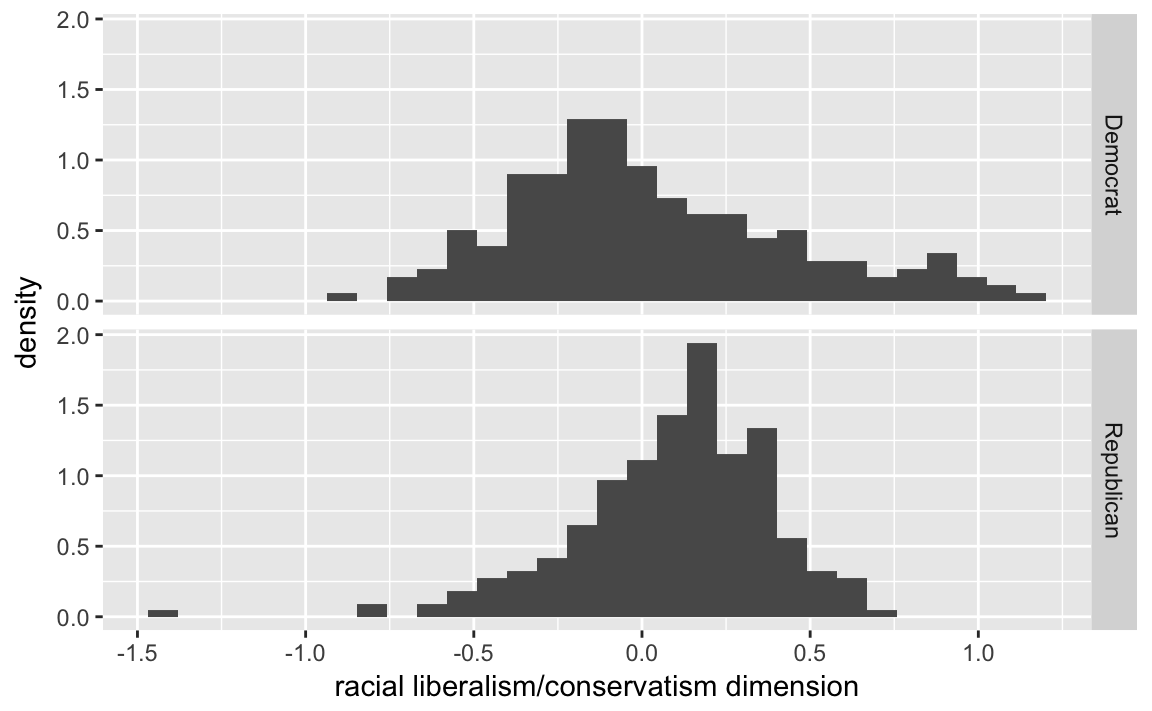
\includegraphics[width=0.7\linewidth]{causality_files/figure-latex/unnamed-chunk-50-1} \end{center}

\hypertarget{descriptive-statistics-for-a-single-variable}{%
\section{Descriptive Statistics for a Single
Variable}\label{descriptive-statistics-for-a-single-variable}}

To calculate the summary for the variables \texttt{wageBefore} and
\texttt{wageAfter} for New Jersey only:

\begin{Shaded}
\begin{Highlighting}[]
\NormalTok{minwage }\OperatorTok
\StringTok{  }\KeywordTok{filter}\NormalTok{(state }\OperatorTok{==}\StringTok{ "NJ"}\NormalTok{) }\OperatorTok
\StringTok{  }\KeywordTok{select}\NormalTok{(wageBefore, wageAfter) }\OperatorTok
\StringTok{  }\KeywordTok{summary}\NormalTok{()}
\CommentTok{#>    wageBefore     wageAfter   }
\CommentTok{#>  Min.   :4.25   Min.   :5.00  }
\CommentTok{#>  1st Qu.:4.25   1st Qu.:5.05  }
\CommentTok{#>  Median :4.50   Median :5.05  }
\CommentTok{#>  Mean   :4.61   Mean   :5.08  }
\CommentTok{#>  3rd Qu.:4.87   3rd Qu.:5.05  }
\CommentTok{#>  Max.   :5.75   Max.   :5.75}
\end{Highlighting}
\end{Shaded}

We calculate the interquartile range for each state's wages after the
passage of the law using the same grouped summarize as we used before:

\begin{Shaded}
\begin{Highlighting}[]
\NormalTok{minwage }\OperatorTok
\StringTok{  }\KeywordTok{group_by}\NormalTok{(state) }\OperatorTok
\StringTok{  }\KeywordTok{summarise}\NormalTok{(}\DataTypeTok{wageAfter =} \KeywordTok{IQR}\NormalTok{(wageAfter),}
            \DataTypeTok{wageBefore =} \KeywordTok{IQR}\NormalTok{(wageBefore))}
\CommentTok{#> # A tibble: 2 x 3}
\CommentTok{#>   state wageAfter wageBefore}
\CommentTok{#>   <chr>     <dbl>      <dbl>}
\CommentTok{#> 1 NJ        0.         0.620}
\CommentTok{#> 2 PA        0.575      0.750}
\end{Highlighting}
\end{Shaded}

Calculate the variance and standard deviation of \texttt{wageAfter} and
\texttt{wageBefore} for each state:

\begin{Shaded}
\begin{Highlighting}[]
\NormalTok{minwage }\OperatorTok
\StringTok{  }\KeywordTok{group_by}\NormalTok{(state) }\OperatorTok
\StringTok{  }\KeywordTok{summarise}\NormalTok{(}\DataTypeTok{wageAfter_sd =} \KeywordTok{sd}\NormalTok{(wageAfter),}
               \DataTypeTok{wageAfter_var =} \KeywordTok{var}\NormalTok{(wageAfter),}
               \DataTypeTok{wageBefore_sd =} \KeywordTok{sd}\NormalTok{(wageBefore),}
               \DataTypeTok{wageBefore_var =} \KeywordTok{var}\NormalTok{(wageBefore))}
\CommentTok{#> # A tibble: 2 x 5}
\CommentTok{#>   state wageAfter_sd wageAfter_var wageBefore_sd wageBefore_var}
\CommentTok{#>   <chr>        <dbl>         <dbl>         <dbl>          <dbl>}
\CommentTok{#> 1 NJ           0.106        0.0112         0.343          0.118}
\CommentTok{#> 2 PA           0.359        0.129          0.358          0.128}
\end{Highlighting}
\end{Shaded}

Here we can see again how using
\href{https://www.rdocumentation.org/packages/dplyr/topics/summarise_at}{summarise\_at}
allows for more compact code to specify variables and summary statistics
that would be the case using just \texttt{summarise}:

\begin{Shaded}
\begin{Highlighting}[]
\NormalTok{minwage }\OperatorTok
\StringTok{  }\KeywordTok{group_by}\NormalTok{(state) }\OperatorTok
\StringTok{  }\KeywordTok{summarise_at}\NormalTok{(}\KeywordTok{vars}\NormalTok{(wageAfter, wageBefore), }\KeywordTok{funs}\NormalTok{(sd, var))}
\CommentTok{#> # A tibble: 2 x 5}
\CommentTok{#>   state wageAfter_sd wageBefore_sd wageAfter_var wageBefore_var}
\CommentTok{#>   <chr>        <dbl>         <dbl>         <dbl>          <dbl>}
\CommentTok{#> 1 NJ           0.106         0.343        0.0112          0.118}
\CommentTok{#> 2 PA           0.359         0.358        0.129           0.128}
\end{Highlighting}
\end{Shaded}

\hypertarget{measurement}{%
\chapter{Measurement}\label{measurement}}

\hypertarget{prerequisites-2}{%
\section*{Prerequisites}\label{prerequisites-2}}
\addcontentsline{toc}{section}{Prerequisites}

\begin{Shaded}
\begin{Highlighting}[]
\KeywordTok{library}\NormalTok{(}\StringTok{"tidyverse"}\NormalTok{)}
\KeywordTok{library}\NormalTok{(}\StringTok{"forcats"}\NormalTok{)}
\KeywordTok{library}\NormalTok{(}\StringTok{"broom"}\NormalTok{)}
\KeywordTok{library}\NormalTok{(}\StringTok{"tidyr"}\NormalTok{)}
\end{Highlighting}
\end{Shaded}

\hypertarget{measuring-civilian-victimization-during-wartime}{%
\section{Measuring Civilian Victimization during
Wartime}\label{measuring-civilian-victimization-during-wartime}}

\begin{Shaded}
\begin{Highlighting}[]
\KeywordTok{data}\NormalTok{(}\StringTok{"afghan"}\NormalTok{, }\DataTypeTok{package =} \StringTok{"qss"}\NormalTok{)}
\end{Highlighting}
\end{Shaded}

Summarize the variables of interest

\begin{Shaded}
\begin{Highlighting}[]
\NormalTok{afghan }\OperatorTok
\StringTok{  }\KeywordTok{select}\NormalTok{(age, educ.years, employed, income) }\OperatorTok
\StringTok{  }\KeywordTok{summary}\NormalTok{()}
\CommentTok{#>       age         educ.years    employed        income         }
\CommentTok{#>  Min.   :15.0   Min.   : 0   Min.   :0.000   Length:2754       }
\CommentTok{#>  1st Qu.:22.0   1st Qu.: 0   1st Qu.:0.000   Class :character  }
\CommentTok{#>  Median :30.0   Median : 1   Median :1.000   Mode  :character  }
\CommentTok{#>  Mean   :32.4   Mean   : 4   Mean   :0.583                     }
\CommentTok{#>  3rd Qu.:40.0   3rd Qu.: 8   3rd Qu.:1.000                     }
\CommentTok{#>  Max.   :80.0   Max.   :18   Max.   :1.000}
\end{Highlighting}
\end{Shaded}

Loading data with either \texttt{data()} or\texttt{read\_csv()} does not
convert strings to factors by default; see below with \texttt{income}.
To get a summary of the different levels, either convert it to a factor
(see \href{http://r4ds.had.co.nz/factors.html}{R4DS Ch 15}), or use
\texttt{count()}:

\begin{Shaded}
\begin{Highlighting}[]
\KeywordTok{count}\NormalTok{(afghan, income)}
\CommentTok{#> # A tibble: 6 x 2}
\CommentTok{#>   income              n}
\CommentTok{#>   <chr>           <int>}
\CommentTok{#> 1 10,001-20,000     616}
\CommentTok{#> 2 2,001-10,000     1420}
\CommentTok{#> 3 20,001-30,000      93}
\CommentTok{#> 4 less than 2,000   457}
\CommentTok{#> 5 over 30,000        14}
\CommentTok{#> 6 <NA>              154}
\end{Highlighting}
\end{Shaded}

Use count to calculate the proportion of respondents who answer that
they were harmed by the ISAF or the Taliban (\texttt{violent.exp.ISAF}
and \texttt{violent.exp.taliban}, respectively):

\begin{Shaded}
\begin{Highlighting}[]
\NormalTok{afghan }\OperatorTok
\StringTok{  }\KeywordTok{group_by}\NormalTok{(violent.exp.ISAF, violent.exp.taliban) }\OperatorTok
\StringTok{  }\KeywordTok{count}\NormalTok{() }\OperatorTok
\StringTok{  }\KeywordTok{ungroup}\NormalTok{() }\OperatorTok
\StringTok{  }\KeywordTok{mutate}\NormalTok{(}\DataTypeTok{prop =}\NormalTok{ n }\OperatorTok{/}\StringTok{ }\KeywordTok{sum}\NormalTok{(n))}
\CommentTok{#> # A tibble: 9 x 4}
\CommentTok{#>   violent.exp.ISAF violent.exp.taliban     n    prop}
\CommentTok{#>              <int>               <int> <int>   <dbl>}
\CommentTok{#> 1                0                   0  1330 0.483  }
\CommentTok{#> 2                0                   1   354 0.129  }
\CommentTok{#> 3                0                  NA    22 0.00799}
\CommentTok{#> 4                1                   0   475 0.172  }
\CommentTok{#> 5                1                   1   526 0.191  }
\CommentTok{#> 6                1                  NA    22 0.00799}
\CommentTok{#> # ... with 3 more rows}
\end{Highlighting}
\end{Shaded}

We need to use \texttt{ungroup()} in order to ensure that
\texttt{sum(n)} sums over the entire dataset as opposed to only within
categories of \texttt{violent.exp.ISAF}. Unlike \texttt{prop.table()},
the code above does not drop missing values. We can drop those values by
adding \texttt{filter()} and \texttt{!is.na()} to test for missing
values in those variables:

\begin{Shaded}
\begin{Highlighting}[]
\NormalTok{afghan }\OperatorTok
\StringTok{  }\KeywordTok{filter}\NormalTok{(}\OperatorTok{!}\KeywordTok{is.na}\NormalTok{(violent.exp.ISAF), }\OperatorTok{!}\KeywordTok{is.na}\NormalTok{(violent.exp.taliban)) }\OperatorTok
\StringTok{  }\KeywordTok{group_by}\NormalTok{(violent.exp.ISAF, violent.exp.taliban) }\OperatorTok
\StringTok{  }\KeywordTok{count}\NormalTok{() }\OperatorTok
\StringTok{  }\KeywordTok{ungroup}\NormalTok{() }\OperatorTok
\StringTok{  }\KeywordTok{mutate}\NormalTok{(}\DataTypeTok{prop =}\NormalTok{ n }\OperatorTok{/}\StringTok{ }\KeywordTok{sum}\NormalTok{(n))}
\CommentTok{#> # A tibble: 4 x 4}
\CommentTok{#>   violent.exp.ISAF violent.exp.taliban     n  prop}
\CommentTok{#>              <int>               <int> <int> <dbl>}
\CommentTok{#> 1                0                   0  1330 0.495}
\CommentTok{#> 2                0                   1   354 0.132}
\CommentTok{#> 3                1                   0   475 0.177}
\CommentTok{#> 4                1                   1   526 0.196}
\end{Highlighting}
\end{Shaded}

\hypertarget{handling-missing-data-in-r}{%
\section{Handling Missing Data in R}\label{handling-missing-data-in-r}}

We already observed the issues with \texttt{NA} values in calculating
the proportion answering the ``experienced violence'' questions. You can
filter rows with specific variables having missing values using
\texttt{filter()} as shown above.

\begin{Shaded}
\begin{Highlighting}[]
\KeywordTok{head}\NormalTok{(afghan}\OperatorTok{$}\NormalTok{income, }\DataTypeTok{n =} \DecValTok{10}\NormalTok{)}
\CommentTok{#>  [1] "2,001-10,000"  "2,001-10,000"  "2,001-10,000"  "2,001-10,000" }
\CommentTok{#>  [5] "2,001-10,000"  NA              "10,001-20,000" "2,001-10,000" }
\CommentTok{#>  [9] "2,001-10,000"  NA}
\KeywordTok{head}\NormalTok{(}\KeywordTok{is.na}\NormalTok{(afghan}\OperatorTok{$}\NormalTok{income), }\DataTypeTok{n =} \DecValTok{10}\NormalTok{)}
\CommentTok{#>  [1] FALSE FALSE FALSE FALSE FALSE  TRUE FALSE FALSE FALSE  TRUE}
\end{Highlighting}
\end{Shaded}

Counts and proportion of missing values of \texttt{income}:

\begin{Shaded}
\begin{Highlighting}[]
\KeywordTok{summarise}\NormalTok{(afghan,}
          \DataTypeTok{n_missing =} \KeywordTok{sum}\NormalTok{(}\KeywordTok{is.na}\NormalTok{(income)),}
          \DataTypeTok{p_missing =} \KeywordTok{mean}\NormalTok{(}\KeywordTok{is.na}\NormalTok{(income)))}
\CommentTok{#>   n_missing p_missing}
\CommentTok{#> 1       154    0.0559}
\end{Highlighting}
\end{Shaded}

Mean, and other functions, do not by default exclude missing values. Use
\texttt{na.rm\ =\ TRUE} in these cases.

\begin{Shaded}
\begin{Highlighting}[]
\NormalTok{x <-}\StringTok{ }\KeywordTok{c}\NormalTok{(}\DecValTok{1}\NormalTok{, }\DecValTok{2}\NormalTok{, }\DecValTok{3}\NormalTok{, }\OtherTok{NA}\NormalTok{)}
\KeywordTok{mean}\NormalTok{(x)}
\CommentTok{#> [1] NA}
\KeywordTok{mean}\NormalTok{(x, }\DataTypeTok{na.rm =} \OtherTok{TRUE}\NormalTok{)}
\CommentTok{#> [1] 2}
\end{Highlighting}
\end{Shaded}

Table of proportions of individuals harmed by the ISAF and Taliban that
includes missing (\texttt{NA}) values:

\begin{Shaded}
\begin{Highlighting}[]
\NormalTok{violent_exp_prop <-}
\StringTok{  }\NormalTok{afghan }\OperatorTok
\StringTok{  }\KeywordTok{group_by}\NormalTok{(violent.exp.ISAF, violent.exp.taliban) }\OperatorTok
\StringTok{  }\KeywordTok{count}\NormalTok{() }\OperatorTok
\StringTok{  }\KeywordTok{ungroup}\NormalTok{() }\OperatorTok
\StringTok{  }\KeywordTok{mutate}\NormalTok{(}\DataTypeTok{prop =}\NormalTok{ n }\OperatorTok{/}\StringTok{ }\KeywordTok{sum}\NormalTok{(n)) }\OperatorTok
\StringTok{  }\KeywordTok{select}\NormalTok{(}\OperatorTok{-}\NormalTok{n)}
\NormalTok{violent_exp_prop}
\CommentTok{#> # A tibble: 9 x 3}
\CommentTok{#>   violent.exp.ISAF violent.exp.taliban    prop}
\CommentTok{#>              <int>               <int>   <dbl>}
\CommentTok{#> 1                0                   0 0.483  }
\CommentTok{#> 2                0                   1 0.129  }
\CommentTok{#> 3                0                  NA 0.00799}
\CommentTok{#> 4                1                   0 0.172  }
\CommentTok{#> 5                1                   1 0.191  }
\CommentTok{#> 6                1                  NA 0.00799}
\CommentTok{#> # ... with 3 more rows}
\end{Highlighting}
\end{Shaded}

The data frame above can be reorganized so that rows are ISAF and the
columns are Taliban as follows:

\begin{Shaded}
\begin{Highlighting}[]
\NormalTok{violent_exp_prop }\OperatorTok
\StringTok{  }\KeywordTok{spread}\NormalTok{(violent.exp.taliban, prop)}
\CommentTok{#> # A tibble: 3 x 4}
\CommentTok{#>   violent.exp.ISAF     `0`     `1`  `<NA>`}
\CommentTok{#>              <int>   <dbl>   <dbl>   <dbl>}
\CommentTok{#> 1                0 0.483   0.129   0.00799}
\CommentTok{#> 2                1 0.172   0.191   0.00799}
\CommentTok{#> 3               NA 0.00254 0.00290 0.00363}
\end{Highlighting}
\end{Shaded}

\texttt{drop\_na} is an alternative to \texttt{na.omit} that allows for
removing missing values,

\begin{Shaded}
\begin{Highlighting}[]
\KeywordTok{drop_na}\NormalTok{(afghan)}
\end{Highlighting}
\end{Shaded}

\textbf{Tip} There are multiple types of
\href{http://r4ds.had.co.nz/vectors.html\#important-types-of-atomic-vector}{missing
values}.

\begin{Shaded}
\begin{Highlighting}[]
\OtherTok{NA}  \CommentTok{# logical}
\CommentTok{#> [1] NA}
\OtherTok{NA_integer_} \CommentTok{# integer}
\CommentTok{#> [1] NA}
\OtherTok{NA_real_} \CommentTok{# double}
\CommentTok{#> [1] NA}
\OtherTok{NA_character_} \CommentTok{# character}
\CommentTok{#> [1] NA}
\end{Highlighting}
\end{Shaded}

In many cases, this distinction does not matter since many functions
will coerce these missing values to the correct vector type. However,
you will need to use these in some tidyverse functions that require the
outputs to be the same type, e.g. \texttt{map()} and most of the other
\href{https://cran.r-project.org/package=purrr}{purrr} functions, and
\texttt{if\_else()}. The code below produces an error, since the
\texttt{TRUE} case returns an integer value (\texttt{x} is an integer),
but the \texttt{FALSE} case does not specify the type of \texttt{NA}.

\begin{Shaded}
\begin{Highlighting}[]
\NormalTok{x <-}\StringTok{ }\DecValTok{1}\OperatorTok{:}\DecValTok{5}
\KeywordTok{class}\NormalTok{(x)}
\CommentTok{#> [1] "integer"}
\KeywordTok{if_else}\NormalTok{(x }\OperatorTok{<}\StringTok{ }\DecValTok{3}\NormalTok{, x, }\OtherTok{NA}\NormalTok{)}
\CommentTok{#> Error: `false` must be type integer, not logical}
\end{Highlighting}
\end{Shaded}

So instead of \texttt{NA}, use \texttt{NA\_integer\_}:

\begin{Shaded}
\begin{Highlighting}[]
\KeywordTok{if_else}\NormalTok{(x }\OperatorTok{<}\StringTok{ }\DecValTok{3}\NormalTok{, x, }\OtherTok{NA_integer_}\NormalTok{)}
\CommentTok{#> [1]  1  2 NA NA NA}
\end{Highlighting}
\end{Shaded}

\hypertarget{visualizing-the-univariate-distribution}{%
\section{Visualizing the Univariate
Distribution}\label{visualizing-the-univariate-distribution}}

\hypertarget{barplot}{%
\subsection{Barplot}\label{barplot}}

\begin{Shaded}
\begin{Highlighting}[]
\NormalTok{afghan <-}
\StringTok{  }\NormalTok{afghan }\OperatorTok
\StringTok{  }\KeywordTok{mutate}\NormalTok{(}\DataTypeTok{violent.exp.ISAF.fct =}
           \KeywordTok{fct_explicit_na}\NormalTok{(}\KeywordTok{fct_recode}\NormalTok{(}\KeywordTok{factor}\NormalTok{(violent.exp.ISAF),}
                                      \DataTypeTok{Harm =} \StringTok{"1"}\NormalTok{, }\StringTok{"No Harm"}\NormalTok{ =}\StringTok{ "0"}\NormalTok{),}
                           \StringTok{"No response"}\NormalTok{))}
\KeywordTok{ggplot}\NormalTok{(afghan, }\KeywordTok{aes}\NormalTok{(}\DataTypeTok{x =}\NormalTok{ violent.exp.ISAF.fct, }\DataTypeTok{y =}\NormalTok{ ..prop.., }\DataTypeTok{group =} \DecValTok{1}\NormalTok{)) }\OperatorTok{+}
\StringTok{  }\KeywordTok{geom_bar}\NormalTok{() }\OperatorTok{+}
\StringTok{  }\KeywordTok{xlab}\NormalTok{(}\StringTok{"Response category"}\NormalTok{) }\OperatorTok{+}
\StringTok{  }\KeywordTok{ylab}\NormalTok{(}\StringTok{"Proportion of respondents"}\NormalTok{) }\OperatorTok{+}
\StringTok{  }\KeywordTok{ggtitle}\NormalTok{(}\StringTok{"Civilian Victimization by the ISAF"}\NormalTok{)}
\end{Highlighting}
\end{Shaded}

\begin{center}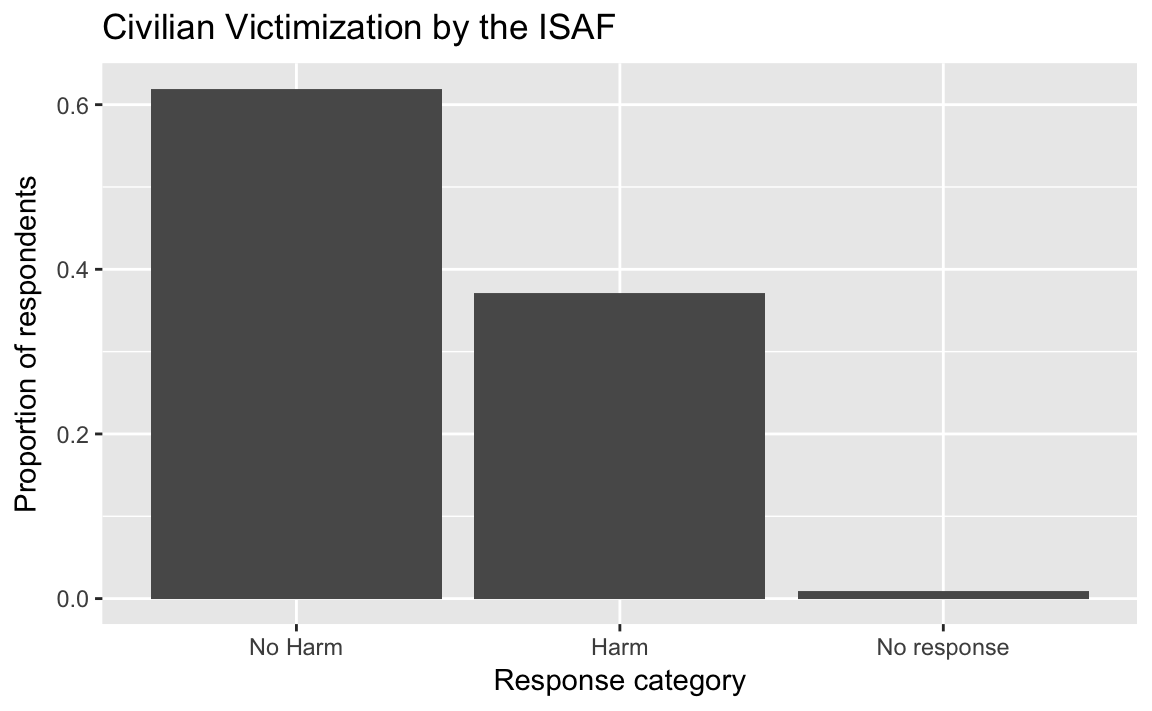
\includegraphics[width=0.7\linewidth]{measurement_files/figure-latex/unnamed-chunk-17-1} \end{center}

\begin{Shaded}
\begin{Highlighting}[]
\NormalTok{afghan <-}
\StringTok{  }\NormalTok{afghan }\OperatorTok
\StringTok{  }\KeywordTok{mutate}\NormalTok{(}\DataTypeTok{violent.exp.taliban.fct =}
           \KeywordTok{fct_explicit_na}\NormalTok{(}\KeywordTok{fct_recode}\NormalTok{(}\KeywordTok{factor}\NormalTok{(violent.exp.taliban),}
                                      \DataTypeTok{Harm =} \StringTok{"1"}\NormalTok{, }\StringTok{"No Harm"}\NormalTok{ =}\StringTok{ "0"}\NormalTok{),}
                           \StringTok{"No response"}\NormalTok{))}
\KeywordTok{ggplot}\NormalTok{(afghan, }\KeywordTok{aes}\NormalTok{(}\DataTypeTok{x =}\NormalTok{ violent.exp.ISAF.fct, }\DataTypeTok{y =}\NormalTok{ ..prop.., }\DataTypeTok{group =} \DecValTok{1}\NormalTok{)) }\OperatorTok{+}
\StringTok{  }\KeywordTok{geom_bar}\NormalTok{() }\OperatorTok{+}
\StringTok{  }\KeywordTok{xlab}\NormalTok{(}\StringTok{"Response category"}\NormalTok{) }\OperatorTok{+}
\StringTok{  }\KeywordTok{ylab}\NormalTok{(}\StringTok{"Proportion of respondents"}\NormalTok{) }\OperatorTok{+}
\StringTok{  }\KeywordTok{ggtitle}\NormalTok{(}\StringTok{"Civilian Victimization by the Taliban"}\NormalTok{)}
\end{Highlighting}
\end{Shaded}

\begin{center}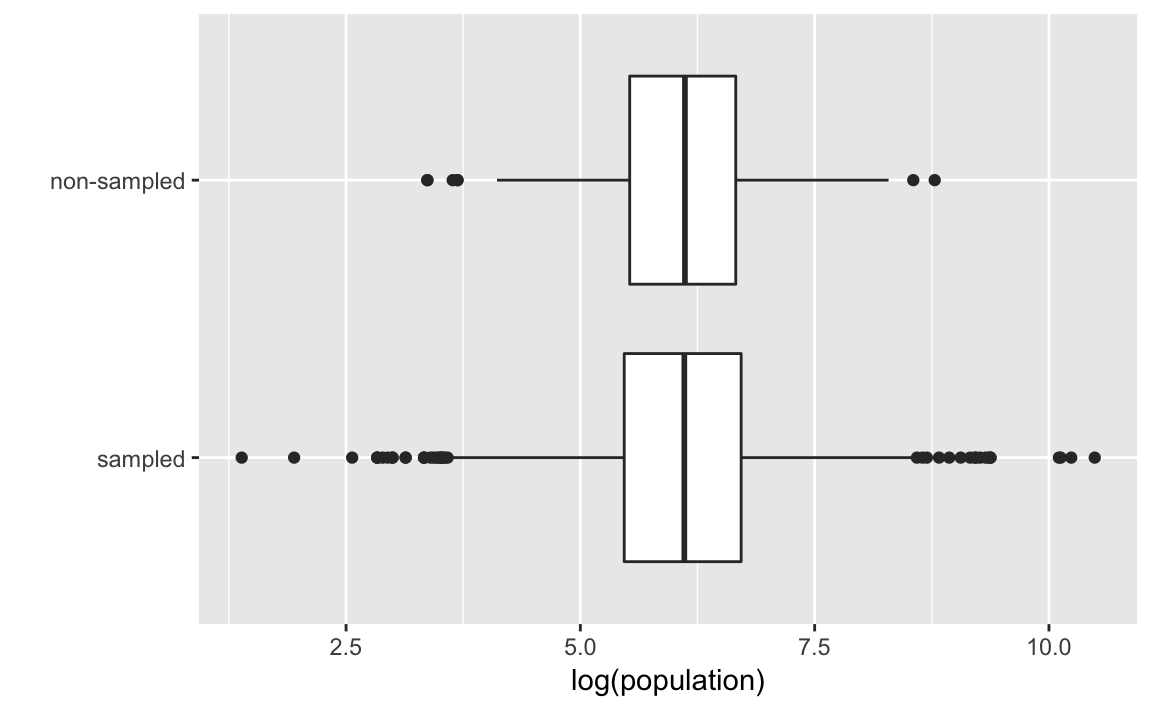
\includegraphics[width=0.7\linewidth]{measurement_files/figure-latex/unnamed-chunk-18-1} \end{center}

Instead of creating two separate box-plots, create a single plot
facetted by ISAF and Taliban:

\begin{Shaded}
\begin{Highlighting}[]
\KeywordTok{select}\NormalTok{(afghan, violent.exp.ISAF, violent.exp.taliban) }\OperatorTok
\StringTok{  }\KeywordTok{gather}\NormalTok{(variable, value) }\OperatorTok
\StringTok{  }\KeywordTok{mutate}\NormalTok{(}\DataTypeTok{value =} \KeywordTok{fct_explicit_na}\NormalTok{(}\KeywordTok{fct_recode}\NormalTok{(}\KeywordTok{factor}\NormalTok{(value),}
                                \DataTypeTok{Harm =} \StringTok{"1"}\NormalTok{, }\StringTok{"No Harm"}\NormalTok{ =}\StringTok{ "0"}\NormalTok{),}
                                \StringTok{"No response"}\NormalTok{),}
         \DataTypeTok{variable =} \KeywordTok{recode}\NormalTok{(variable,}
                           \DataTypeTok{violent.exp.ISAF =} \StringTok{"ISAF"}\NormalTok{,}
                           \DataTypeTok{violent.exp.taliban =} \StringTok{"Taliban"}\NormalTok{)) }\OperatorTok
\StringTok{  }\KeywordTok{ggplot}\NormalTok{(}\KeywordTok{aes}\NormalTok{(}\DataTypeTok{x =}\NormalTok{ value, }\DataTypeTok{y =}\NormalTok{ ..prop.., }\DataTypeTok{group =} \DecValTok{1}\NormalTok{)) }\OperatorTok{+}
\StringTok{  }\KeywordTok{geom_bar}\NormalTok{() }\OperatorTok{+}
\StringTok{  }\KeywordTok{facet_wrap}\NormalTok{(}\OperatorTok{~}\StringTok{ }\NormalTok{variable, }\DataTypeTok{ncol =} \DecValTok{1}\NormalTok{) }\OperatorTok{+}
\StringTok{  }\KeywordTok{xlab}\NormalTok{(}\StringTok{"Response category"}\NormalTok{) }\OperatorTok{+}
\StringTok{  }\KeywordTok{ylab}\NormalTok{(}\StringTok{"Proportion of respondents"}\NormalTok{) }\OperatorTok{+}
\StringTok{  }\KeywordTok{ggtitle}\NormalTok{(}\StringTok{"Civilian Victimization"}\NormalTok{)}
\end{Highlighting}
\end{Shaded}

\begin{center}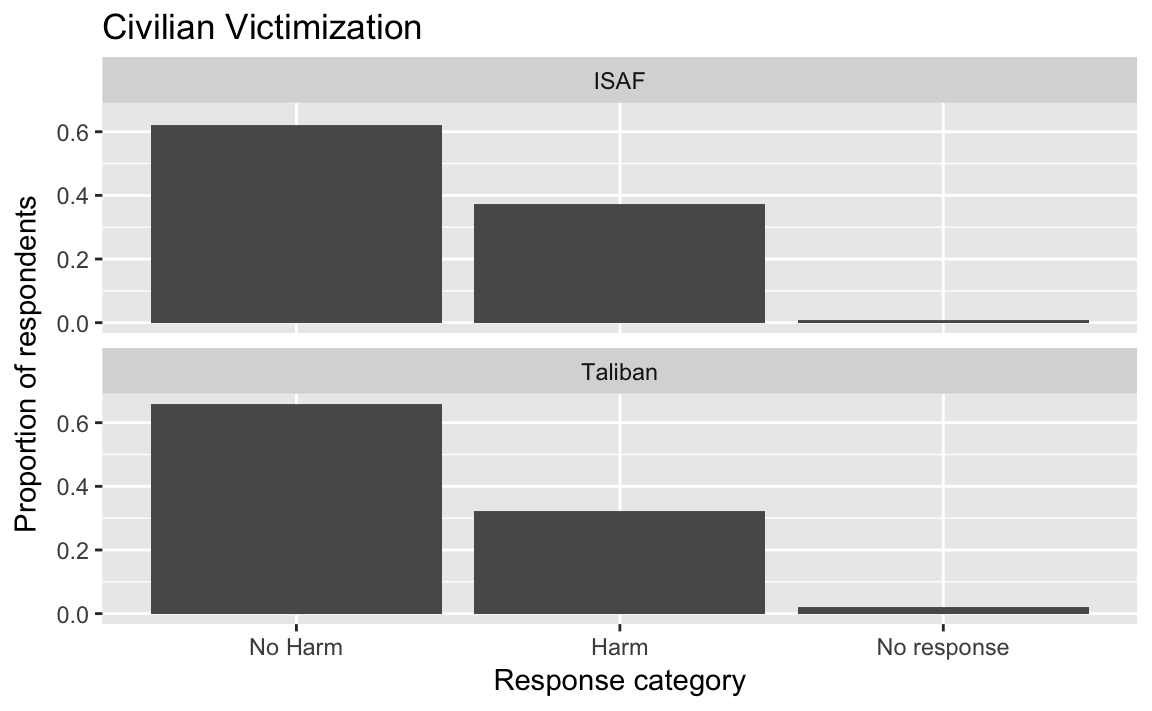
\includegraphics[width=0.7\linewidth]{measurement_files/figure-latex/unnamed-chunk-19-1} \end{center}

This plot could improved by plotting the two values simultaneously to be
able to better compare them. This will require creating a data frame
that has the following columns: perpetrator (\texttt{ISAF},
\texttt{Taliban}) and response (\texttt{No\ Harm}, \texttt{Harm},
\texttt{No\ response}).

\begin{Shaded}
\begin{Highlighting}[]
\NormalTok{violent_exp <-}
\StringTok{  }\NormalTok{afghan }\OperatorTok
\StringTok{  }\KeywordTok{select}\NormalTok{(violent.exp.ISAF, violent.exp.taliban) }\OperatorTok
\StringTok{  }\KeywordTok{gather}\NormalTok{(perpetrator, response) }\OperatorTok
\StringTok{  }\KeywordTok{mutate}\NormalTok{(}\DataTypeTok{perpetrator =} \KeywordTok{str_replace}\NormalTok{(perpetrator, }\StringTok{"violent}\CharTok{\textbackslash{}\textbackslash{}}\StringTok{.exp}\CharTok{\textbackslash{}\textbackslash{}}\StringTok{."}\NormalTok{, }\StringTok{""}\NormalTok{),}
         \DataTypeTok{perpetrator =} \KeywordTok{str_replace}\NormalTok{(perpetrator, }\StringTok{"taliban"}\NormalTok{, }\StringTok{"Taliban"}\NormalTok{),}
         \DataTypeTok{response =} \KeywordTok{fct_recode}\NormalTok{(}\KeywordTok{factor}\NormalTok{(response), }\StringTok{"Harm"}\NormalTok{ =}\StringTok{ "1"}\NormalTok{, }\StringTok{"No Harm"}\NormalTok{ =}\StringTok{ "0"}\NormalTok{),}
         \DataTypeTok{response =} \KeywordTok{fct_explicit_na}\NormalTok{(response, }\StringTok{"No response"}\NormalTok{),}
         \DataTypeTok{response =} \KeywordTok{fct_relevel}\NormalTok{(response, }\KeywordTok{c}\NormalTok{(}\StringTok{"No response"}\NormalTok{, }\StringTok{"No Harm"}\NormalTok{))}
\NormalTok{         ) }\OperatorTok
\StringTok{  }\KeywordTok{count}\NormalTok{(perpetrator, response) }\OperatorTok
\StringTok{  }\KeywordTok{mutate}\NormalTok{(}\DataTypeTok{prop =}\NormalTok{ n }\OperatorTok{/}\StringTok{ }\KeywordTok{sum}\NormalTok{(n))}
\KeywordTok{ggplot}\NormalTok{(violent_exp, }\KeywordTok{aes}\NormalTok{(}\DataTypeTok{x =}\NormalTok{ prop, }\DataTypeTok{y =}\NormalTok{ response, }\DataTypeTok{color =}\NormalTok{ perpetrator)) }\OperatorTok{+}
\StringTok{  }\KeywordTok{geom_point}\NormalTok{() }\OperatorTok{+}
\StringTok{  }\KeywordTok{scale_color_manual}\NormalTok{(}\DataTypeTok{values =} \KeywordTok{c}\NormalTok{(}\DataTypeTok{ISAF =} \StringTok{"green"}\NormalTok{, }\DataTypeTok{Taliban =} \StringTok{"black"}\NormalTok{))}
\end{Highlighting}
\end{Shaded}

\begin{center}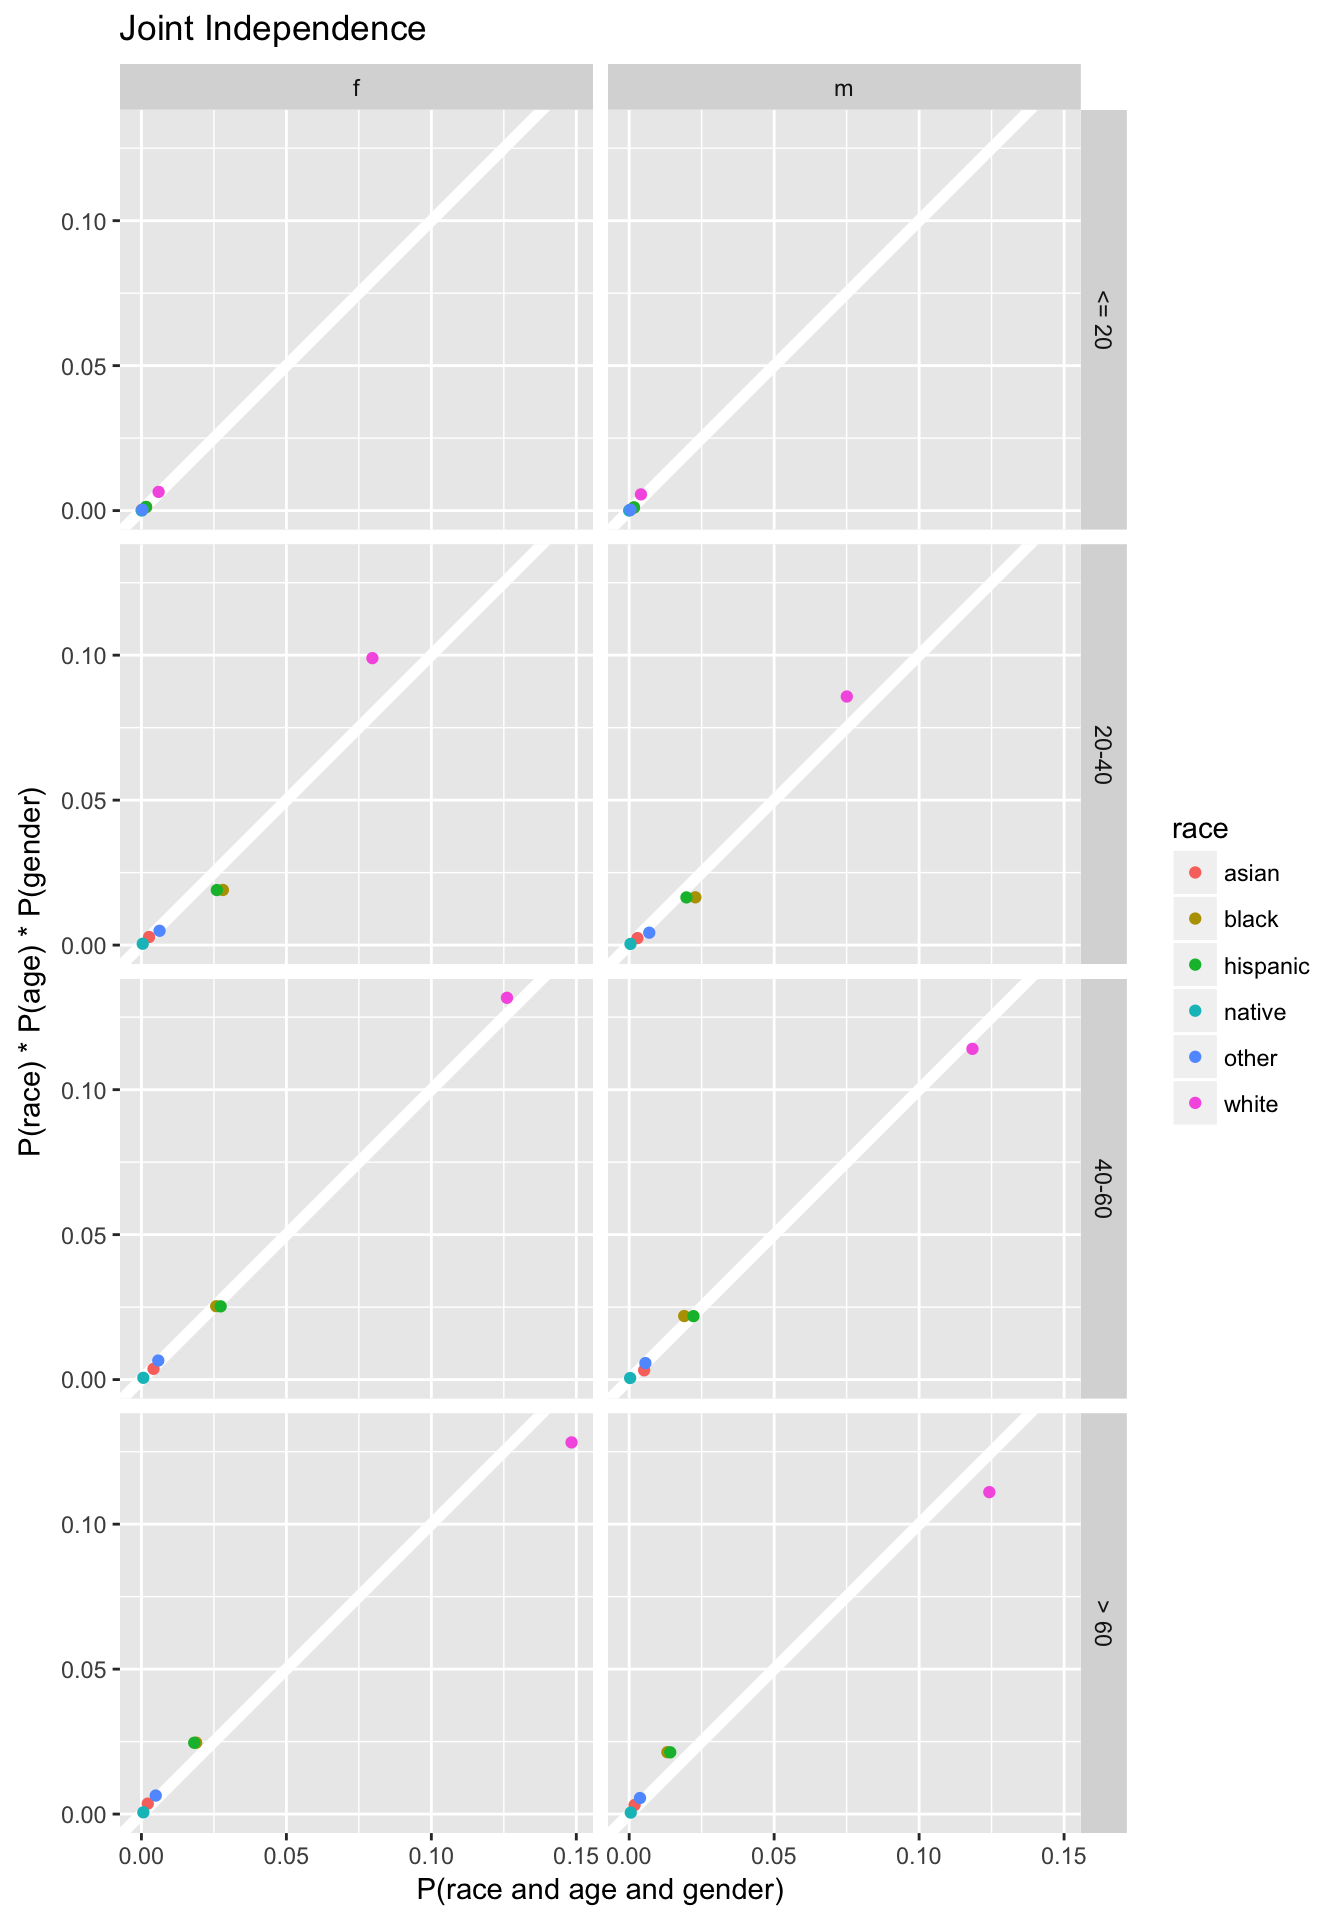
\includegraphics[width=0.7\linewidth]{measurement_files/figure-latex/unnamed-chunk-20-1} \end{center}

Black was chosen for the Taliban, and Green for ISAF because they are
the colors of their respective
\href{https://en.wikipedia.org/wiki/International_Security_Assistance_Force}{flags}.

\hypertarget{histogram}{%
\subsection{Histogram}\label{histogram}}

See the documentation for
\href{https://www.rdocumentation.org/packages/ggplot2/topics/geom_histogram}{geom\_histogram}.

\begin{Shaded}
\begin{Highlighting}[]
\KeywordTok{ggplot}\NormalTok{(afghan, }\KeywordTok{aes}\NormalTok{(}\DataTypeTok{x =}\NormalTok{ age, }\DataTypeTok{y =}\NormalTok{ ..density..)) }\OperatorTok{+}
\StringTok{  }\KeywordTok{geom_histogram}\NormalTok{(}\DataTypeTok{binwidth =} \DecValTok{5}\NormalTok{, }\DataTypeTok{boundary =} \DecValTok{0}\NormalTok{) }\OperatorTok{+}
\StringTok{  }\KeywordTok{scale_x_continuous}\NormalTok{(}\DataTypeTok{breaks =} \KeywordTok{seq}\NormalTok{(}\DecValTok{20}\NormalTok{, }\DecValTok{80}\NormalTok{, }\DataTypeTok{by =} \DecValTok{10}\NormalTok{)) }\OperatorTok{+}
\StringTok{  }\KeywordTok{labs}\NormalTok{(}\DataTypeTok{title =} \StringTok{"Distribution of respondent's age"}\NormalTok{,}
       \DataTypeTok{y =} \StringTok{"Age"}\NormalTok{, }\DataTypeTok{x =} \StringTok{"Density"}\NormalTok{)}
\end{Highlighting}
\end{Shaded}

\begin{center}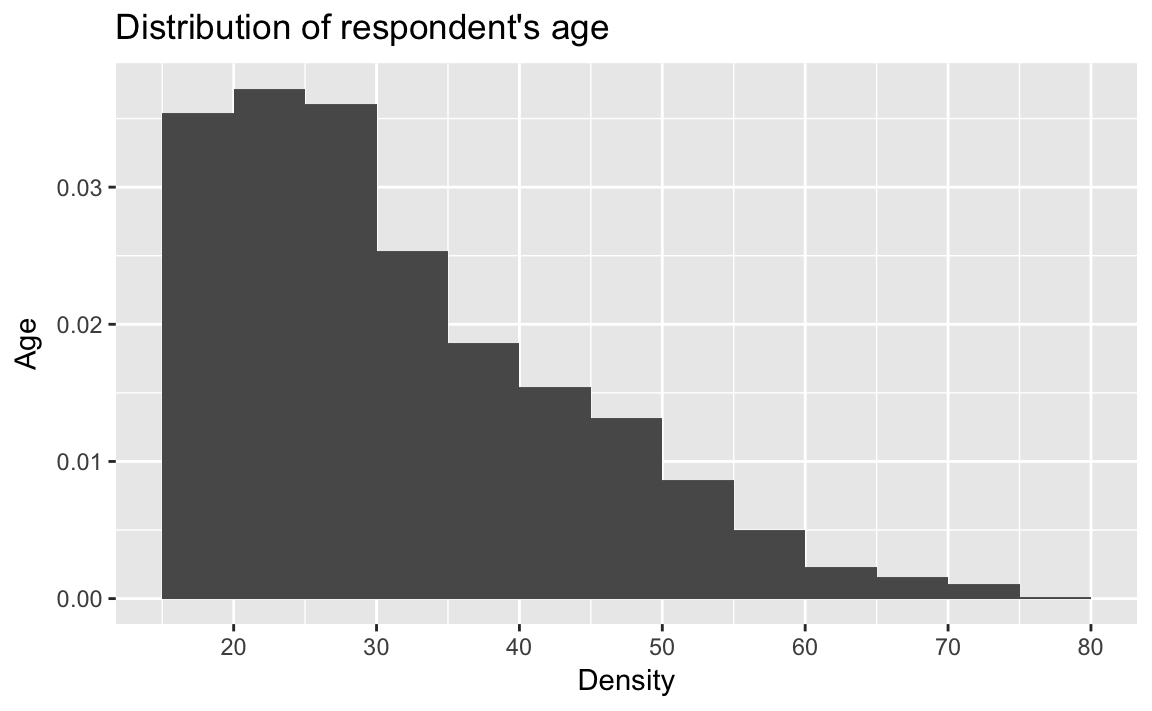
\includegraphics[width=0.7\linewidth]{measurement_files/figure-latex/hist_age-1} \end{center}

\begin{Shaded}
\begin{Highlighting}[]
\KeywordTok{ggplot}\NormalTok{(afghan, }\KeywordTok{aes}\NormalTok{(}\DataTypeTok{x =}\NormalTok{ educ.years, }\DataTypeTok{y =}\NormalTok{ ..density..)) }\OperatorTok{+}
\StringTok{  }\KeywordTok{geom_histogram}\NormalTok{(}\DataTypeTok{binwidth =} \DecValTok{1}\NormalTok{, }\DataTypeTok{center =} \DecValTok{0}\NormalTok{) }\OperatorTok{+}
\StringTok{  }\KeywordTok{geom_vline}\NormalTok{(}\DataTypeTok{xintercept =} \KeywordTok{median}\NormalTok{(afghan}\OperatorTok{$}\NormalTok{educ.years),}
             \DataTypeTok{color =} \StringTok{"white"}\NormalTok{, }\DataTypeTok{size =} \DecValTok{2}\NormalTok{) }\OperatorTok{+}
\StringTok{  }\KeywordTok{annotate}\NormalTok{(}\StringTok{"text"}\NormalTok{, }\DataTypeTok{x =} \KeywordTok{median}\NormalTok{(afghan}\OperatorTok{$}\NormalTok{educ.years),}
           \DataTypeTok{y =} \FloatTok{0.2}\NormalTok{, }\DataTypeTok{label =} \StringTok{"median"}\NormalTok{, }\DataTypeTok{hjust =} \DecValTok{0}\NormalTok{) }\OperatorTok{+}
\StringTok{  }\KeywordTok{labs}\NormalTok{(}\DataTypeTok{title =} \StringTok{"Distribution of respondent's education"}\NormalTok{,}
       \DataTypeTok{x =} \StringTok{"Years of education"}\NormalTok{,}
       \DataTypeTok{y =} \StringTok{"Density"}\NormalTok{)}
  
\end{Highlighting}
\end{Shaded}

\begin{center}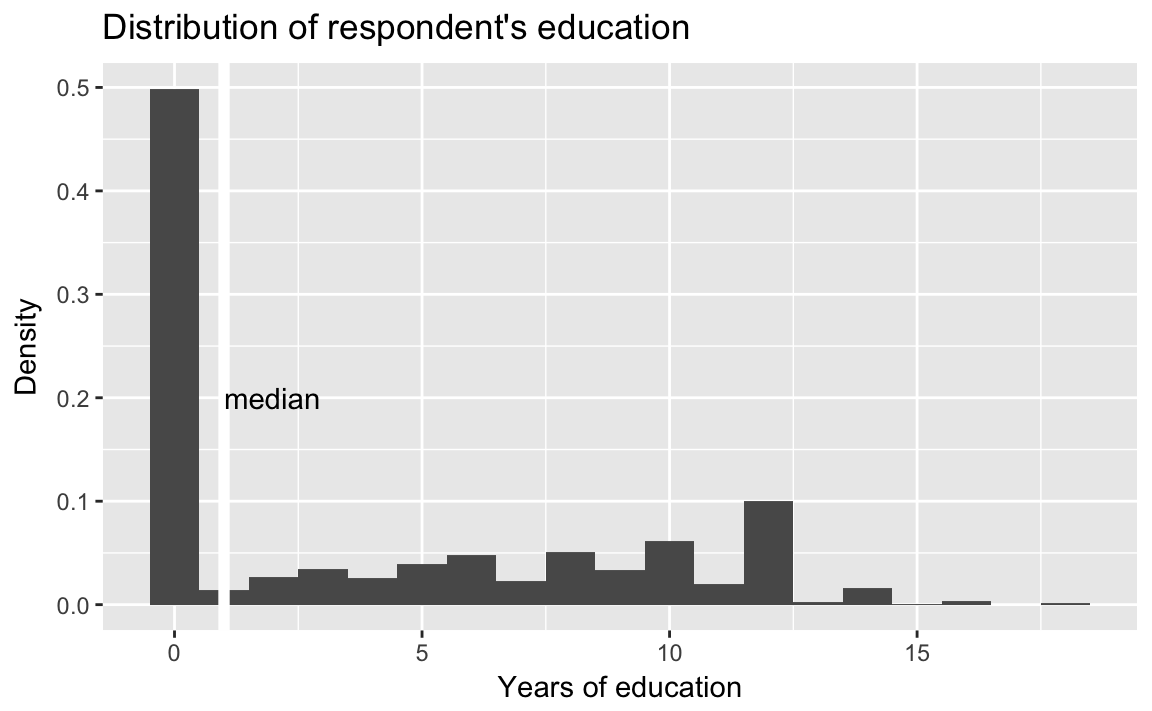
\includegraphics[width=0.7\linewidth]{measurement_files/figure-latex/unnamed-chunk-21-1} \end{center}

There are several alternatives to the histogram.

Density plots
(\href{https://www.rdocumentation.org/packages/ggplot2/topics/geom_density}{geom\_density}):

\begin{Shaded}
\begin{Highlighting}[]
\NormalTok{dens_plot <-}\StringTok{ }\KeywordTok{ggplot}\NormalTok{(afghan, }\KeywordTok{aes}\NormalTok{(}\DataTypeTok{x =}\NormalTok{ age)) }\OperatorTok{+}
\StringTok{  }\KeywordTok{geom_density}\NormalTok{() }\OperatorTok{+}
\StringTok{  }\KeywordTok{scale_x_continuous}\NormalTok{(}\DataTypeTok{breaks =} \KeywordTok{seq}\NormalTok{(}\DecValTok{20}\NormalTok{, }\DecValTok{80}\NormalTok{, }\DataTypeTok{by =} \DecValTok{10}\NormalTok{)) }\OperatorTok{+}
\StringTok{  }\KeywordTok{labs}\NormalTok{(}\DataTypeTok{title =} \StringTok{"Distribution of respondent's age"}\NormalTok{,}
       \DataTypeTok{y =} \StringTok{"Age"}\NormalTok{, }\DataTypeTok{x =} \StringTok{"Density"}\NormalTok{)}
\NormalTok{dens_plot}
\end{Highlighting}
\end{Shaded}

\begin{center}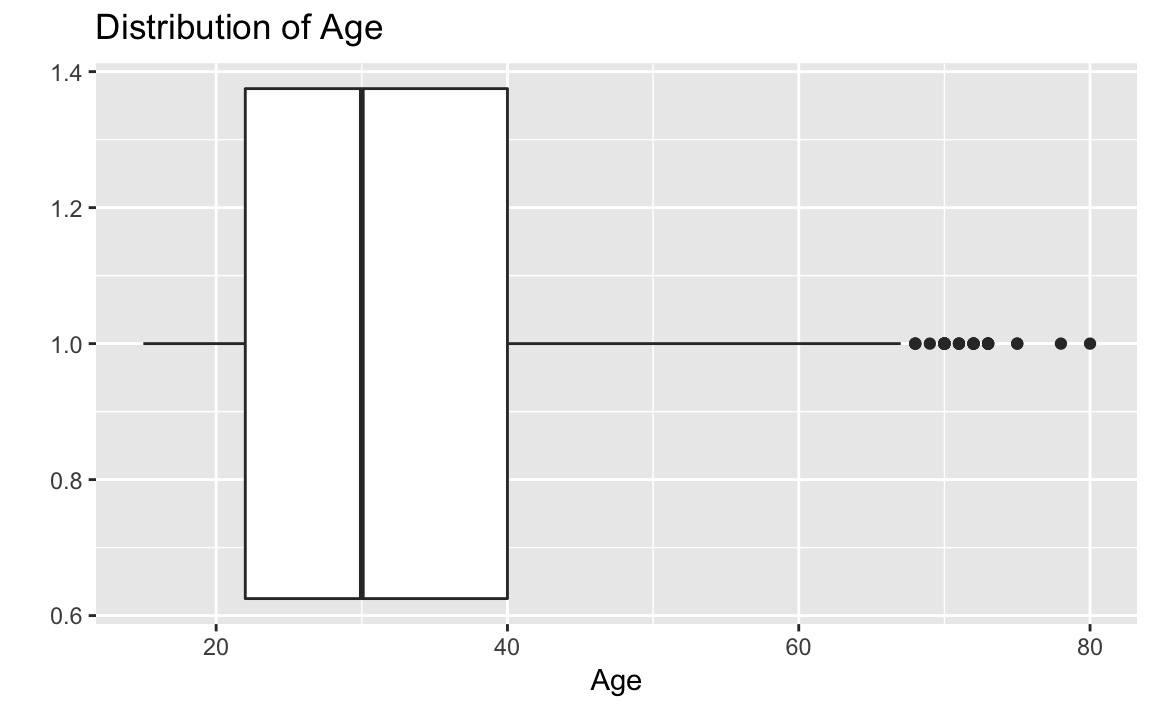
\includegraphics[width=0.7\linewidth]{measurement_files/figure-latex/unnamed-chunk-22-1} \end{center}

which can be combined with a
\href{https://www.rdocumentation.org/packages/ggplot2/topics/geom_rug}{geom\_rug}
to create a rug plot, which puts small lines on the axis to represent
the value of each observation. It can be combined with a scatter or
density plot to add extra detail. Adjust the \texttt{alpha} to modify
the color transparency of the rug and address overplotting.

\begin{Shaded}
\begin{Highlighting}[]
\NormalTok{dens_plot }\OperatorTok{+}\StringTok{ }\KeywordTok{geom_rug}\NormalTok{(}\DataTypeTok{alpha =} \FloatTok{.2}\NormalTok{)}
\end{Highlighting}
\end{Shaded}

\begin{center}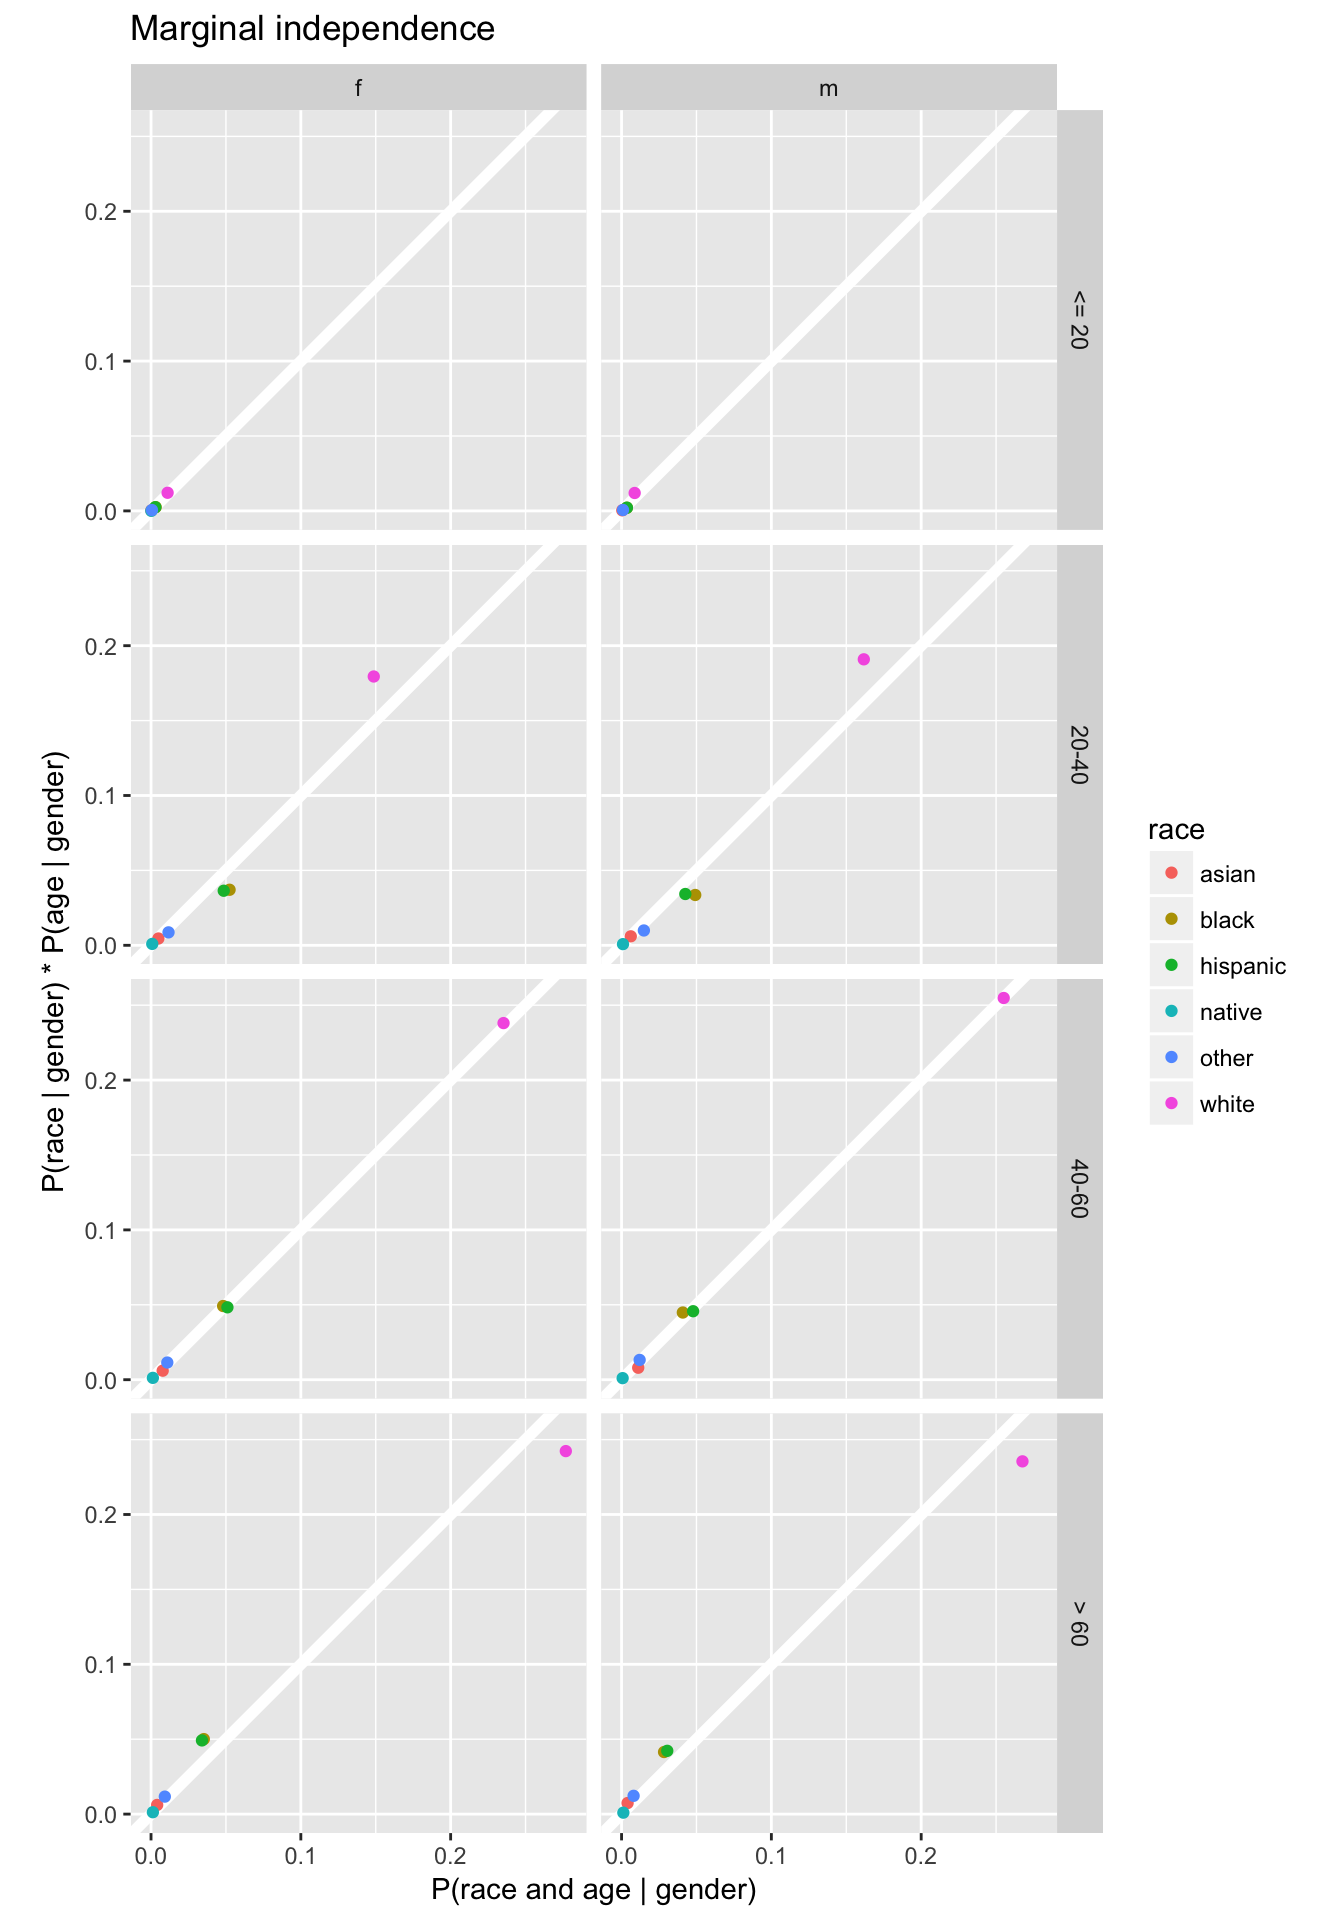
\includegraphics[width=0.7\linewidth]{measurement_files/figure-latex/unnamed-chunk-23-1} \end{center}

Frequency polygons
(\href{https://www.rdocumentation.org/packages/ggplot2/topics/geom_freqpoly}{geom\_freqpoly}):
See \href{http://r4ds.had.co.nz/}{R for Data Science}
\href{http://r4ds.had.co.nz/exploratory-data-analysis.html}{EDA}.

\begin{Shaded}
\begin{Highlighting}[]
\KeywordTok{ggplot}\NormalTok{(afghan, }\KeywordTok{aes}\NormalTok{(}\DataTypeTok{x =}\NormalTok{ age)) }\OperatorTok{+}
\StringTok{  }\KeywordTok{geom_freqpoly}\NormalTok{() }\OperatorTok{+}
\StringTok{  }\KeywordTok{scale_x_continuous}\NormalTok{(}\DataTypeTok{breaks =} \KeywordTok{seq}\NormalTok{(}\DecValTok{20}\NormalTok{, }\DecValTok{80}\NormalTok{, }\DataTypeTok{by =} \DecValTok{10}\NormalTok{)) }\OperatorTok{+}
\StringTok{  }\KeywordTok{labs}\NormalTok{(}\DataTypeTok{title =} \StringTok{"Distribution of respondent's age"}\NormalTok{,}
       \DataTypeTok{y =} \StringTok{"Age"}\NormalTok{, }\DataTypeTok{x =} \StringTok{"Density"}\NormalTok{)}
\CommentTok{#> `stat_bin()` using `bins = 30`. Pick better value with `binwidth`.}
\end{Highlighting}
\end{Shaded}

\begin{center}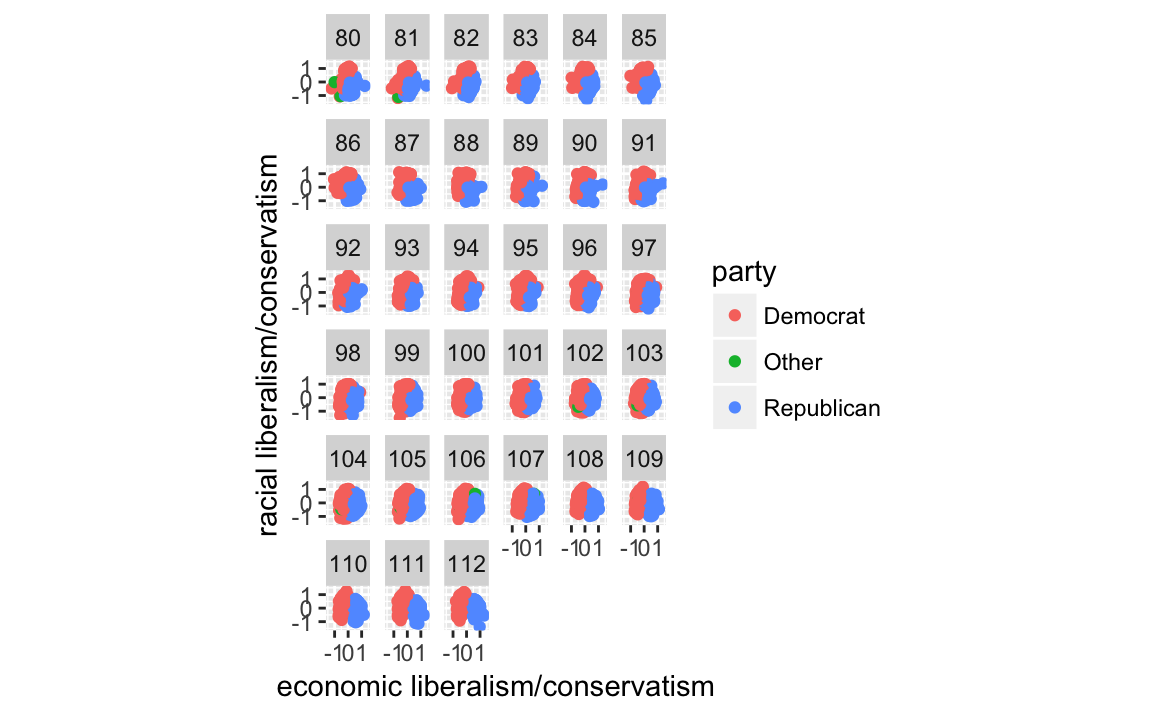
\includegraphics[width=0.7\linewidth]{measurement_files/figure-latex/unnamed-chunk-24-1} \end{center}

\hypertarget{boxplot}{%
\subsection{Boxplot}\label{boxplot}}

See the documentation for
\href{https://www.rdocumentation.org/packages/ggplot2/topics/geom_boxplot}{geom\_boxplot}.

\begin{Shaded}
\begin{Highlighting}[]
\KeywordTok{ggplot}\NormalTok{(afghan, }\KeywordTok{aes}\NormalTok{(}\DataTypeTok{x =} \DecValTok{1}\NormalTok{, }\DataTypeTok{y =}\NormalTok{ age)) }\OperatorTok{+}
\StringTok{  }\KeywordTok{geom_boxplot}\NormalTok{() }\OperatorTok{+}
\StringTok{  }\KeywordTok{coord_flip}\NormalTok{() }\OperatorTok{+}
\StringTok{  }\KeywordTok{labs}\NormalTok{(}\DataTypeTok{y =} \StringTok{"Age"}\NormalTok{, }\DataTypeTok{x =} \StringTok{""}\NormalTok{, }\DataTypeTok{title =} \StringTok{"Distribution of Age"}\NormalTok{)}
\end{Highlighting}
\end{Shaded}

\begin{center}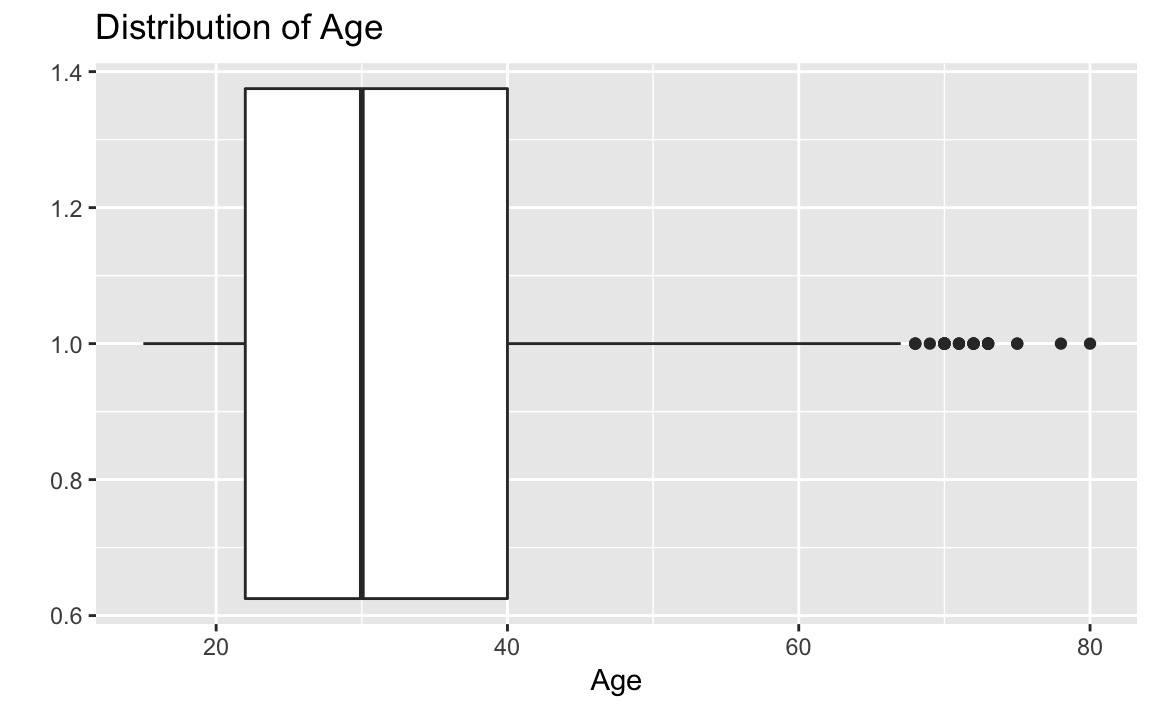
\includegraphics[width=0.7\linewidth]{measurement_files/figure-latex/unnamed-chunk-25-1} \end{center}

\begin{Shaded}
\begin{Highlighting}[]
\KeywordTok{ggplot}\NormalTok{(afghan, }\KeywordTok{aes}\NormalTok{(}\DataTypeTok{y =}\NormalTok{ educ.years, }\DataTypeTok{x =}\NormalTok{ province)) }\OperatorTok{+}
\StringTok{  }\KeywordTok{geom_boxplot}\NormalTok{() }\OperatorTok{+}
\StringTok{  }\KeywordTok{coord_flip}\NormalTok{() }\OperatorTok{+}
\StringTok{  }\KeywordTok{labs}\NormalTok{(}\DataTypeTok{x =} \StringTok{"Province"}\NormalTok{, }\DataTypeTok{y =} \StringTok{"Years of education"}\NormalTok{,}
       \DataTypeTok{title =} \StringTok{"Education by Province"}\NormalTok{)}
\end{Highlighting}
\end{Shaded}

\begin{center}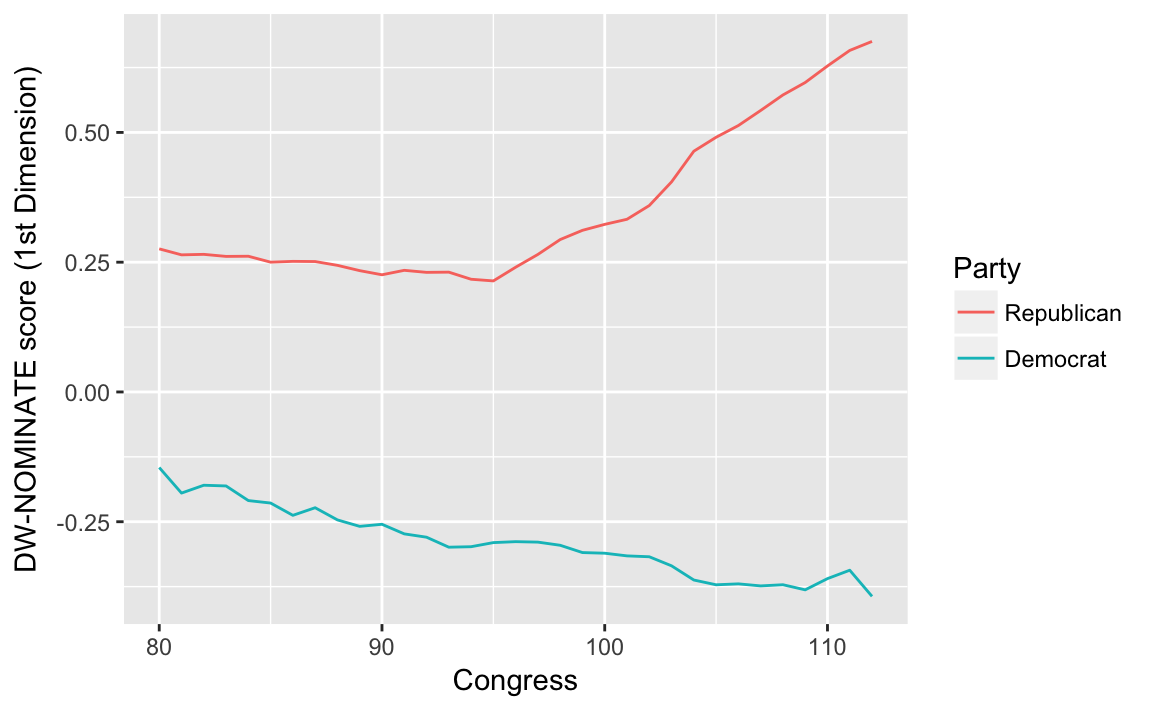
\includegraphics[width=0.7\linewidth]{measurement_files/figure-latex/unnamed-chunk-26-1} \end{center}

Helmand and Uruzgan have much lower levels of education than the other
provinces, and also report higher levels of violence.

\begin{Shaded}
\begin{Highlighting}[]
\NormalTok{afghan }\OperatorTok
\StringTok{  }\KeywordTok{group_by}\NormalTok{(province) }\OperatorTok
\StringTok{  }\KeywordTok{summarise}\NormalTok{(}\DataTypeTok{educ.years =} \KeywordTok{mean}\NormalTok{(educ.years, }\DataTypeTok{na.rm =} \OtherTok{TRUE}\NormalTok{),}
            \DataTypeTok{violent.exp.taliban =}
              \KeywordTok{mean}\NormalTok{(violent.exp.taliban, }\DataTypeTok{na.rm =} \OtherTok{TRUE}\NormalTok{),}
            \DataTypeTok{violent.exp.ISAF =}
              \KeywordTok{mean}\NormalTok{(violent.exp.ISAF, }\DataTypeTok{na.rm =} \OtherTok{TRUE}\NormalTok{)) }\OperatorTok
\StringTok{  }\KeywordTok{arrange}\NormalTok{(educ.years)}
\CommentTok{#> # A tibble: 5 x 4}
\CommentTok{#>   province educ.years violent.exp.taliban violent.exp.ISAF}
\CommentTok{#>   <chr>         <dbl>               <dbl>            <dbl>}
\CommentTok{#> 1 Uruzgan        1.04              0.455             0.496}
\CommentTok{#> 2 Helmand        1.60              0.504             0.541}
\CommentTok{#> 3 Khost          5.79              0.233             0.242}
\CommentTok{#> 4 Kunar          5.93              0.303             0.399}
\CommentTok{#> 5 Logar          6.70              0.0802            0.144}
\end{Highlighting}
\end{Shaded}

An alternatives to the traditional boxplot:

The Tufte boxplot:

\begin{Shaded}
\begin{Highlighting}[]
\KeywordTok{library}\NormalTok{(}\StringTok{"ggthemes"}\NormalTok{)}
\KeywordTok{ggplot}\NormalTok{(afghan, }\KeywordTok{aes}\NormalTok{(}\DataTypeTok{y =}\NormalTok{ educ.years, }\DataTypeTok{x =}\NormalTok{ province)) }\OperatorTok{+}
\StringTok{  }\KeywordTok{geom_tufteboxplot}\NormalTok{() }\OperatorTok{+}
\StringTok{  }\KeywordTok{coord_flip}\NormalTok{() }\OperatorTok{+}
\StringTok{  }\KeywordTok{labs}\NormalTok{(}\DataTypeTok{x =} \StringTok{"Province"}\NormalTok{, }\DataTypeTok{y =} \StringTok{"Years of education"}\NormalTok{,}
       \DataTypeTok{title =} \StringTok{"Education by Province"}\NormalTok{)}
\end{Highlighting}
\end{Shaded}

\begin{center}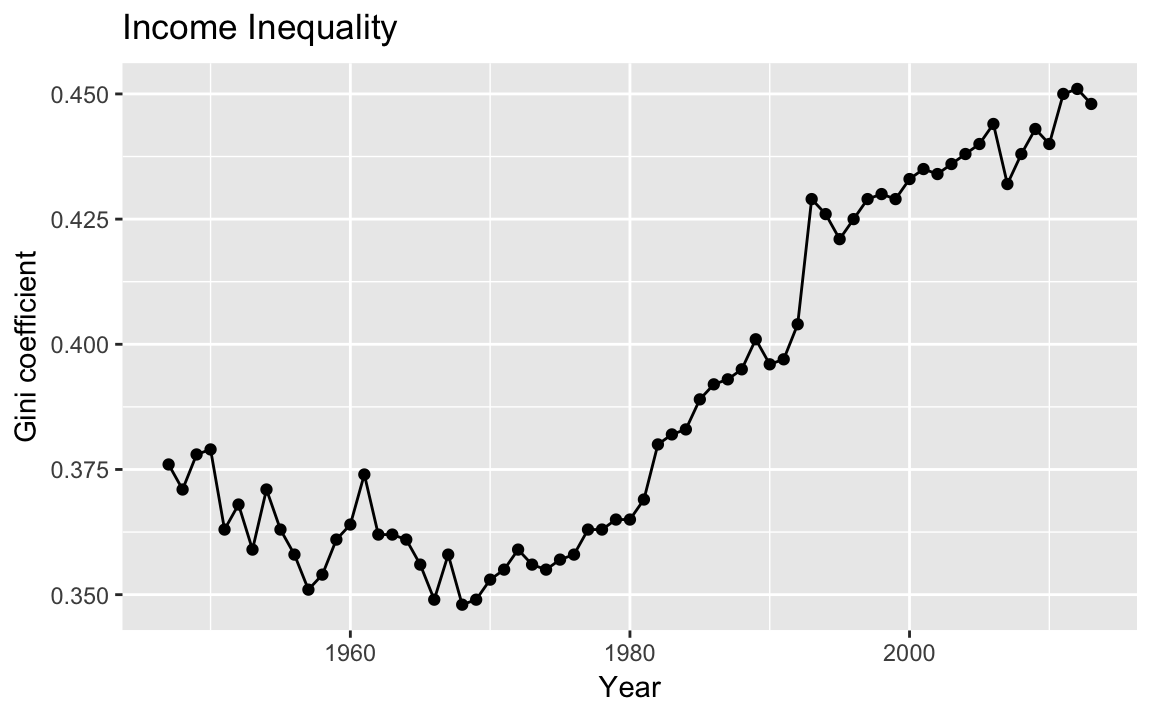
\includegraphics[width=0.7\linewidth]{measurement_files/figure-latex/unnamed-chunk-28-1} \end{center}

Dot plot with jitter and adjusted alpha to avoid overplotting:

\begin{Shaded}
\begin{Highlighting}[]
\KeywordTok{ggplot}\NormalTok{(afghan, }\KeywordTok{aes}\NormalTok{(}\DataTypeTok{y =}\NormalTok{ educ.years, }\DataTypeTok{x =}\NormalTok{ province)) }\OperatorTok{+}
\StringTok{  }\KeywordTok{geom_point}\NormalTok{(}\DataTypeTok{position =} \KeywordTok{position_jitter}\NormalTok{(}\DataTypeTok{width =} \FloatTok{0.25}\NormalTok{, }\DataTypeTok{height =} \DecValTok{0}\NormalTok{),}
             \DataTypeTok{alpha =} \FloatTok{.2}\NormalTok{) }\OperatorTok{+}
\StringTok{  }\KeywordTok{coord_flip}\NormalTok{() }\OperatorTok{+}
\StringTok{  }\KeywordTok{labs}\NormalTok{(}\DataTypeTok{x =} \StringTok{"Province"}\NormalTok{, }\DataTypeTok{y =} \StringTok{"Years of education"}\NormalTok{,}
       \DataTypeTok{title =} \StringTok{"Education by Province"}\NormalTok{)}
\end{Highlighting}
\end{Shaded}

\begin{center}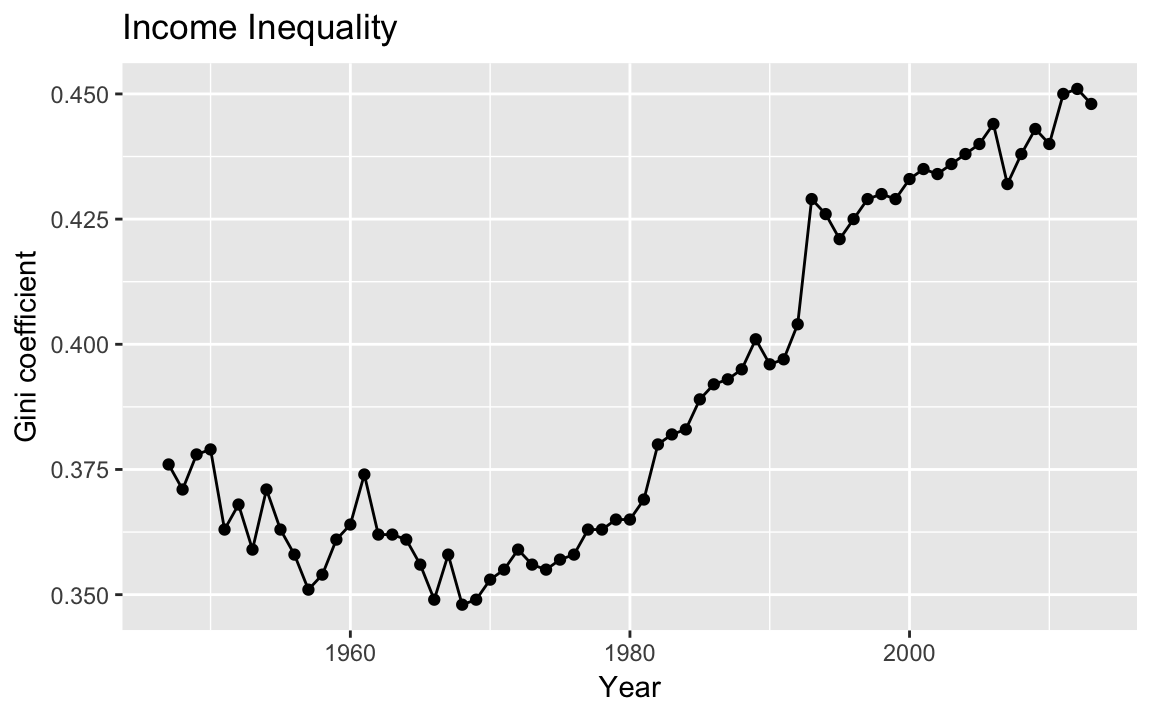
\includegraphics[width=0.7\linewidth]{measurement_files/figure-latex/unnamed-chunk-29-1} \end{center}

A violin plot:

\begin{Shaded}
\begin{Highlighting}[]
\KeywordTok{ggplot}\NormalTok{(afghan, }\KeywordTok{aes}\NormalTok{(}\DataTypeTok{y =}\NormalTok{ educ.years, }\DataTypeTok{x =}\NormalTok{ province)) }\OperatorTok{+}
\StringTok{  }\KeywordTok{geom_violin}\NormalTok{() }\OperatorTok{+}
\StringTok{  }\KeywordTok{coord_flip}\NormalTok{() }\OperatorTok{+}
\StringTok{  }\KeywordTok{labs}\NormalTok{(}\DataTypeTok{x =} \StringTok{"Province"}\NormalTok{, }\DataTypeTok{y =} \StringTok{"Years of education"}\NormalTok{,}
       \DataTypeTok{title =} \StringTok{"Education by Province"}\NormalTok{)}
\end{Highlighting}
\end{Shaded}

\begin{center}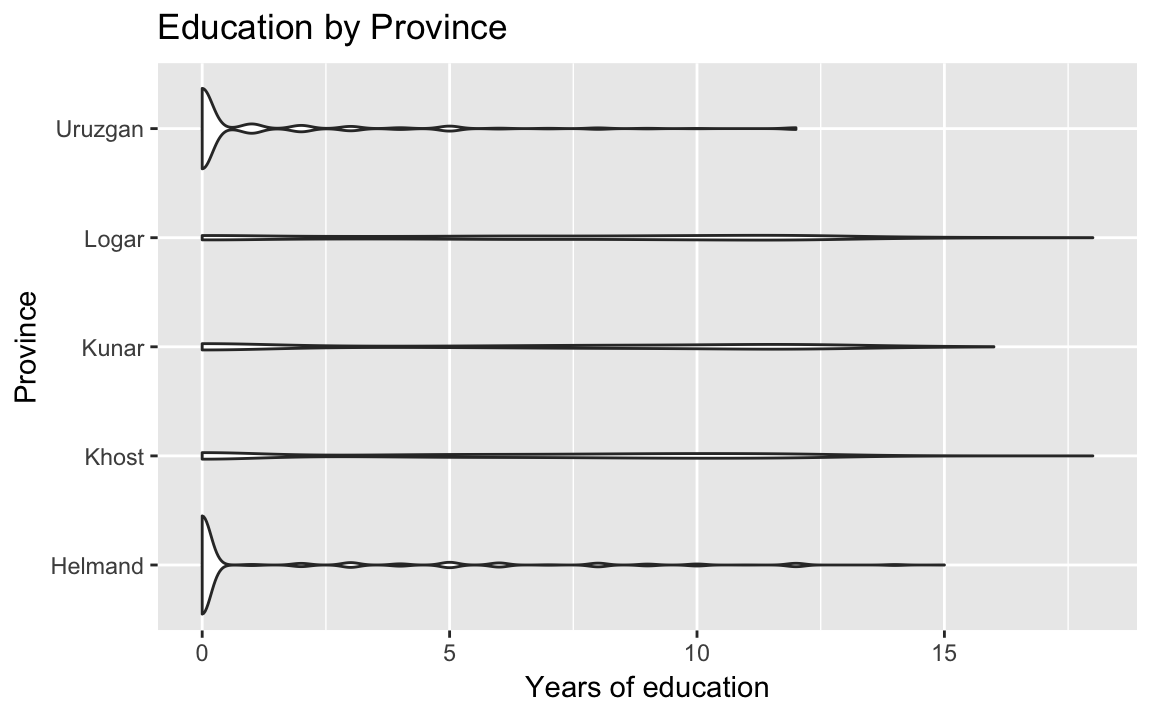
\includegraphics[width=0.7\linewidth]{measurement_files/figure-latex/unnamed-chunk-30-1} \end{center}

\hypertarget{printing-and-saving-graphics}{%
\subsection{Printing and saving
graphics}\label{printing-and-saving-graphics}}

Use the function \texttt{rdoc\ ("ggplot2",\ "ggsave")} to save
\href{https://cran.r-project.org/package=ggplot2}{ggplot2} graphics.
Also, R Markdown files have their own means of creating and saving plots
created by code-chunks.

\hypertarget{survey-sampling}{%
\section{Survey Sampling}\label{survey-sampling}}

\hypertarget{the-role-of-randomization}{%
\subsection{The Role of Randomization}\label{the-role-of-randomization}}

\begin{Shaded}
\begin{Highlighting}[]
\KeywordTok{data}\NormalTok{(}\StringTok{"afghan.village"}\NormalTok{, }\DataTypeTok{package =} \StringTok{"qss"}\NormalTok{)}
\end{Highlighting}
\end{Shaded}

Box-plots of altitude

\begin{Shaded}
\begin{Highlighting}[]
\KeywordTok{ggplot}\NormalTok{(afghan.village, }\KeywordTok{aes}\NormalTok{(}\DataTypeTok{x =} \KeywordTok{factor}\NormalTok{(village.surveyed,}
                                      \DataTypeTok{labels =} \KeywordTok{c}\NormalTok{(}\StringTok{"sampled"}\NormalTok{, }\StringTok{"non-sampled"}\NormalTok{)),}
                           \DataTypeTok{y =}\NormalTok{ altitude)) }\OperatorTok{+}
\StringTok{  }\KeywordTok{geom_boxplot}\NormalTok{() }\OperatorTok{+}
\StringTok{  }\KeywordTok{labs}\NormalTok{(}\DataTypeTok{y =} \StringTok{"Altitude (meter)"}\NormalTok{, }\DataTypeTok{x =} \StringTok{""}\NormalTok{) }\OperatorTok{+}
\StringTok{  }\KeywordTok{coord_flip}\NormalTok{()}
\end{Highlighting}
\end{Shaded}

\begin{center}\includegraphics[width=0.7\linewidth]{measurement_files/figure-latex/unnamed-chunk-32-1} \end{center}

Box plots log-population values of sampled and non-sampled

\begin{Shaded}
\begin{Highlighting}[]
\KeywordTok{ggplot}\NormalTok{(afghan.village, }\KeywordTok{aes}\NormalTok{(}\DataTypeTok{x =} \KeywordTok{factor}\NormalTok{(village.surveyed,}
                                      \DataTypeTok{labels =} \KeywordTok{c}\NormalTok{(}\StringTok{"sampled"}\NormalTok{, }\StringTok{"non-sampled"}\NormalTok{)),}
                           \DataTypeTok{y =} \KeywordTok{log}\NormalTok{(population))) }\OperatorTok{+}
\StringTok{  }\KeywordTok{geom_boxplot}\NormalTok{() }\OperatorTok{+}
\StringTok{  }\KeywordTok{labs}\NormalTok{(}\DataTypeTok{y =} \StringTok{"log(population)"}\NormalTok{, }\DataTypeTok{x =} \StringTok{""}\NormalTok{) }\OperatorTok{+}
\StringTok{  }\KeywordTok{coord_flip}\NormalTok{()}
\end{Highlighting}
\end{Shaded}

\begin{center}\includegraphics[width=0.7\linewidth]{measurement_files/figure-latex/unnamed-chunk-33-1} \end{center}

You can also compare these distributions by plotting their densities:

\begin{Shaded}
\begin{Highlighting}[]
\KeywordTok{ggplot}\NormalTok{(afghan.village, }\KeywordTok{aes}\NormalTok{(}\DataTypeTok{colour =} \KeywordTok{factor}\NormalTok{(village.surveyed,}
                                      \DataTypeTok{labels =} \KeywordTok{c}\NormalTok{(}\StringTok{"sampled"}\NormalTok{, }\StringTok{"non-sampled"}\NormalTok{)),}
                           \DataTypeTok{x =} \KeywordTok{log}\NormalTok{(population))) }\OperatorTok{+}
\StringTok{  }\KeywordTok{geom_density}\NormalTok{() }\OperatorTok{+}
\StringTok{  }\KeywordTok{geom_rug}\NormalTok{() }\OperatorTok{+}
\StringTok{  }\KeywordTok{labs}\NormalTok{(}\DataTypeTok{x =} \StringTok{"log(population)"}\NormalTok{, }\DataTypeTok{colour =} \StringTok{""}\NormalTok{)}
\end{Highlighting}
\end{Shaded}

\begin{center}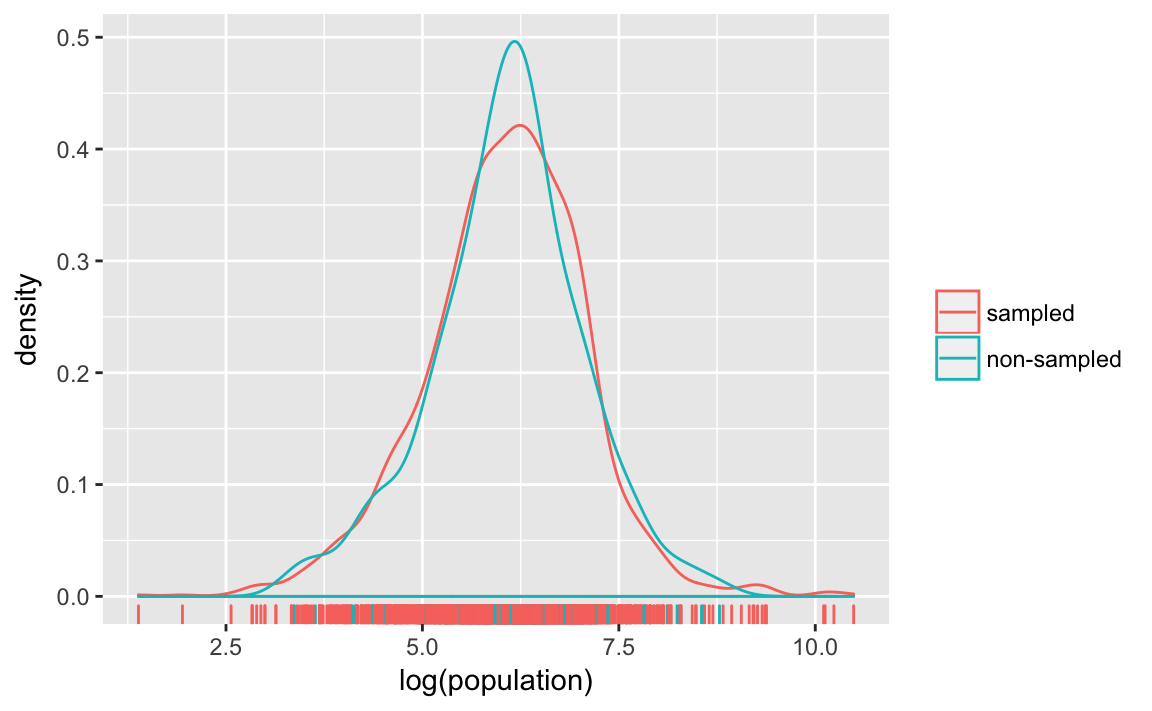
\includegraphics[width=0.7\linewidth]{measurement_files/figure-latex/unnamed-chunk-34-1} \end{center}

\hypertarget{non-response-and-other-sources-of-bias}{%
\subsection{Non-response and other sources of
bias}\label{non-response-and-other-sources-of-bias}}

Calculate the rates of item non-response by province to the question
about civilian victimization by ISAF and Taliban forces
(\texttt{violent.exp.ISAF} and \texttt{violent.exp.taliban}):

\begin{Shaded}
\begin{Highlighting}[]
\NormalTok{afghan }\OperatorTok
\StringTok{  }\KeywordTok{group_by}\NormalTok{(province) }\OperatorTok
\StringTok{  }\KeywordTok{summarise}\NormalTok{(}\DataTypeTok{ISAF =} \KeywordTok{mean}\NormalTok{(}\KeywordTok{is.na}\NormalTok{(violent.exp.ISAF)),}
            \DataTypeTok{taliban =} \KeywordTok{mean}\NormalTok{(}\KeywordTok{is.na}\NormalTok{(violent.exp.taliban))) }\OperatorTok
\StringTok{  }\KeywordTok{arrange}\NormalTok{(}\OperatorTok{-}\NormalTok{ISAF)}
\CommentTok{#> # A tibble: 5 x 3}
\CommentTok{#>   province    ISAF taliban}
\CommentTok{#>   <chr>      <dbl>   <dbl>}
\CommentTok{#> 1 Uruzgan  0.0207  0.0620 }
\CommentTok{#> 2 Helmand  0.0164  0.0304 }
\CommentTok{#> 3 Khost    0.00476 0.00635}
\CommentTok{#> 4 Kunar    0.      0.     }
\CommentTok{#> 5 Logar    0.      0.}
\end{Highlighting}
\end{Shaded}

Calculate the proportion who support the ISAF using the difference in
means between the ISAF and control groups:

\begin{Shaded}
\begin{Highlighting}[]
\NormalTok{(}\KeywordTok{mean}\NormalTok{(}\KeywordTok{filter}\NormalTok{(afghan, list.group }\OperatorTok{==}\StringTok{ "ISAF"}\NormalTok{)}\OperatorTok{$}\NormalTok{list.response) }\OperatorTok{-}
\StringTok{  }\KeywordTok{mean}\NormalTok{(}\KeywordTok{filter}\NormalTok{(afghan, list.group }\OperatorTok{==}\StringTok{ "control"}\NormalTok{)}\OperatorTok{$}\NormalTok{list.response))}
\CommentTok{#> [1] 0.049}
\end{Highlighting}
\end{Shaded}

To calculate the table responses to the list experiment in the control,
ISAF, and Taliban groups:

\begin{Shaded}
\begin{Highlighting}[]
\NormalTok{afghan }\OperatorTok
\StringTok{  }\KeywordTok{group_by}\NormalTok{(list.response, list.group) }\OperatorTok
\StringTok{  }\KeywordTok{count}\NormalTok{() }\OperatorTok
\StringTok{  }\KeywordTok{glimpse}\NormalTok{() }\OperatorTok
\StringTok{  }\KeywordTok{spread}\NormalTok{(list.group, n, }\DataTypeTok{fill =} \DecValTok{0}\NormalTok{)}
\CommentTok{#> Observations: 12}
\CommentTok{#> Variables: 3}
\CommentTok{#> $ list.response <int> 0, 0, 1, 1, 1, 2, 2, 2, 3, 3, 3, 4}
\CommentTok{#> $ list.group    <chr> "control", "ISAF", "control", "ISAF", "taliban",...}
\CommentTok{#> $ n             <int> 188, 174, 265, 278, 433, 265, 260, 287, 200, 182...}
\CommentTok{#> # A tibble: 5 x 4}
\CommentTok{#> # Groups:   list.response [5]}
\CommentTok{#>   list.response control  ISAF taliban}
\CommentTok{#>           <int>   <dbl> <dbl>   <dbl>}
\CommentTok{#> 1             0    188.  174.      0.}
\CommentTok{#> 2             1    265.  278.    433.}
\CommentTok{#> 3             2    265.  260.    287.}
\CommentTok{#> 4             3    200.  182.    198.}
\CommentTok{#> 5             4      0.   24.      0.}
\end{Highlighting}
\end{Shaded}

\hypertarget{measuring-political-polarization}{%
\section{Measuring Political
Polarization}\label{measuring-political-polarization}}

\begin{Shaded}
\begin{Highlighting}[]
\KeywordTok{data}\NormalTok{(}\StringTok{"congress"}\NormalTok{, }\DataTypeTok{package =} \StringTok{"qss"}\NormalTok{)}
\end{Highlighting}
\end{Shaded}

\begin{Shaded}
\begin{Highlighting}[]
\KeywordTok{glimpse}\NormalTok{(congress)}
\CommentTok{#> Observations: 14,552}
\CommentTok{#> Variables: 7}
\CommentTok{#> $ congress <int> 80, 80, 80, 80, 80, 80, 80, 80, 80, 80, 80, 80, 80, 8...}
\CommentTok{#> $ district <int> 0, 1, 2, 3, 4, 5, 6, 7, 8, 9, 98, 98, 1, 2, 3, 4, 5, ...}
\CommentTok{#> $ state    <chr> "USA", "ALABAMA", "ALABAMA", "ALABAMA", "ALABAMA", "A...}
\CommentTok{#> $ party    <chr> "Democrat", "Democrat", "Democrat", "Democrat", "Demo...}
\CommentTok{#> $ name     <chr> "TRUMAN", "BOYKIN  F.", "GRANT  G.", "ANDREWS  G.", "...}
\CommentTok{#> $ dwnom1   <dbl> -0.276, -0.026, -0.042, -0.008, -0.082, -0.170, -0.12...}
\CommentTok{#> $ dwnom2   <dbl> 0.016, 0.796, 0.999, 1.005, 1.066, 0.870, 0.990, 0.89...}
\end{Highlighting}
\end{Shaded}

\begin{Shaded}
\begin{Highlighting}[]
\NormalTok{q <-}
\StringTok{  }\NormalTok{congress }\OperatorTok
\StringTok{  }\KeywordTok{filter}\NormalTok{(congress }\OperatorTok\StringTok{ }\KeywordTok{c}\NormalTok{(}\DecValTok{80}\NormalTok{, }\DecValTok{112}\NormalTok{),}
\NormalTok{         party }\OperatorTok\StringTok{ }\KeywordTok{c}\NormalTok{(}\StringTok{"Democrat"}\NormalTok{, }\StringTok{"Republican"}\NormalTok{)) }\OperatorTok
\StringTok{  }\KeywordTok{ggplot}\NormalTok{(}\KeywordTok{aes}\NormalTok{(}\DataTypeTok{x =}\NormalTok{ dwnom1, }\DataTypeTok{y =}\NormalTok{ dwnom2, }\DataTypeTok{colour =}\NormalTok{ party)) }\OperatorTok{+}
\StringTok{  }\KeywordTok{geom_point}\NormalTok{() }\OperatorTok{+}
\StringTok{  }\KeywordTok{facet_wrap}\NormalTok{(}\OperatorTok{~}\StringTok{ }\NormalTok{congress) }\OperatorTok{+}
\StringTok{  }\KeywordTok{coord_fixed}\NormalTok{() }\OperatorTok{+}
\StringTok{  }\KeywordTok{scale_y_continuous}\NormalTok{(}\StringTok{"racial liberalism/conservatism"}\NormalTok{,}
                     \DataTypeTok{limits =} \KeywordTok{c}\NormalTok{(}\OperatorTok{-}\FloatTok{1.5}\NormalTok{, }\FloatTok{1.5}\NormalTok{)) }\OperatorTok{+}
\StringTok{  }\KeywordTok{scale_x_continuous}\NormalTok{(}\StringTok{"economic liberalism/conservatism"}\NormalTok{,}
                     \DataTypeTok{limits =} \KeywordTok{c}\NormalTok{(}\OperatorTok{-}\FloatTok{1.5}\NormalTok{, }\FloatTok{1.5}\NormalTok{))}
\NormalTok{q}
\end{Highlighting}
\end{Shaded}

\begin{center}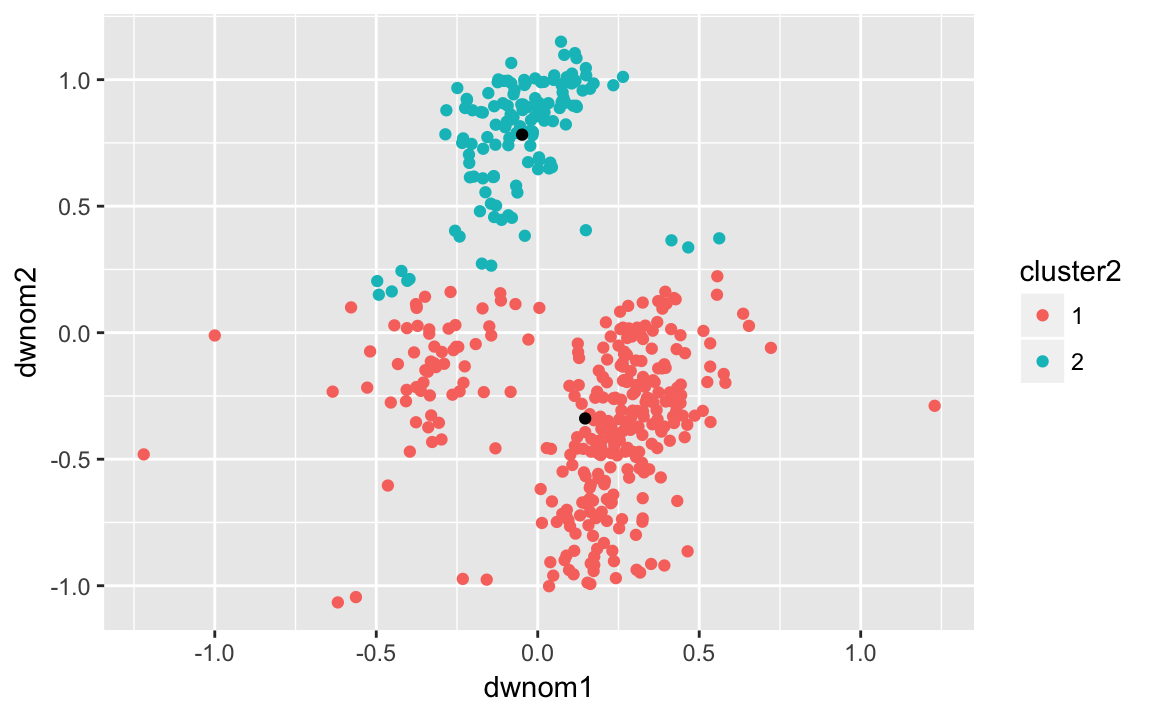
\includegraphics[width=0.7\linewidth]{measurement_files/figure-latex/unnamed-chunk-40-1} \end{center}

However, since there are colors associated with Democrats (blue) and
Republicans (blue), we should use them rather than the defaults. There's
some evidence that using semantically-resonant colors can help decoding
data visualizations (See
\href{http://vis.stanford.edu/files/2013-SemanticColor-EuroVis.pdf}{Lin,
et al.~2013}). Since I'll reuse the scale several times, I'll save it in
a variable.

\begin{Shaded}
\begin{Highlighting}[]
\NormalTok{scale_colour_parties <-}
\StringTok{  }\KeywordTok{scale_colour_manual}\NormalTok{(}\DataTypeTok{values =} \KeywordTok{c}\NormalTok{(}\DataTypeTok{Democrat =} \StringTok{"blue"}\NormalTok{,}
                                 \DataTypeTok{Republican =} \StringTok{"red"}\NormalTok{,}
                                 \DataTypeTok{Other =} \StringTok{"green"}\NormalTok{))}
\NormalTok{q }\OperatorTok{+}\StringTok{ }\NormalTok{scale_colour_parties}
\end{Highlighting}
\end{Shaded}

\begin{center}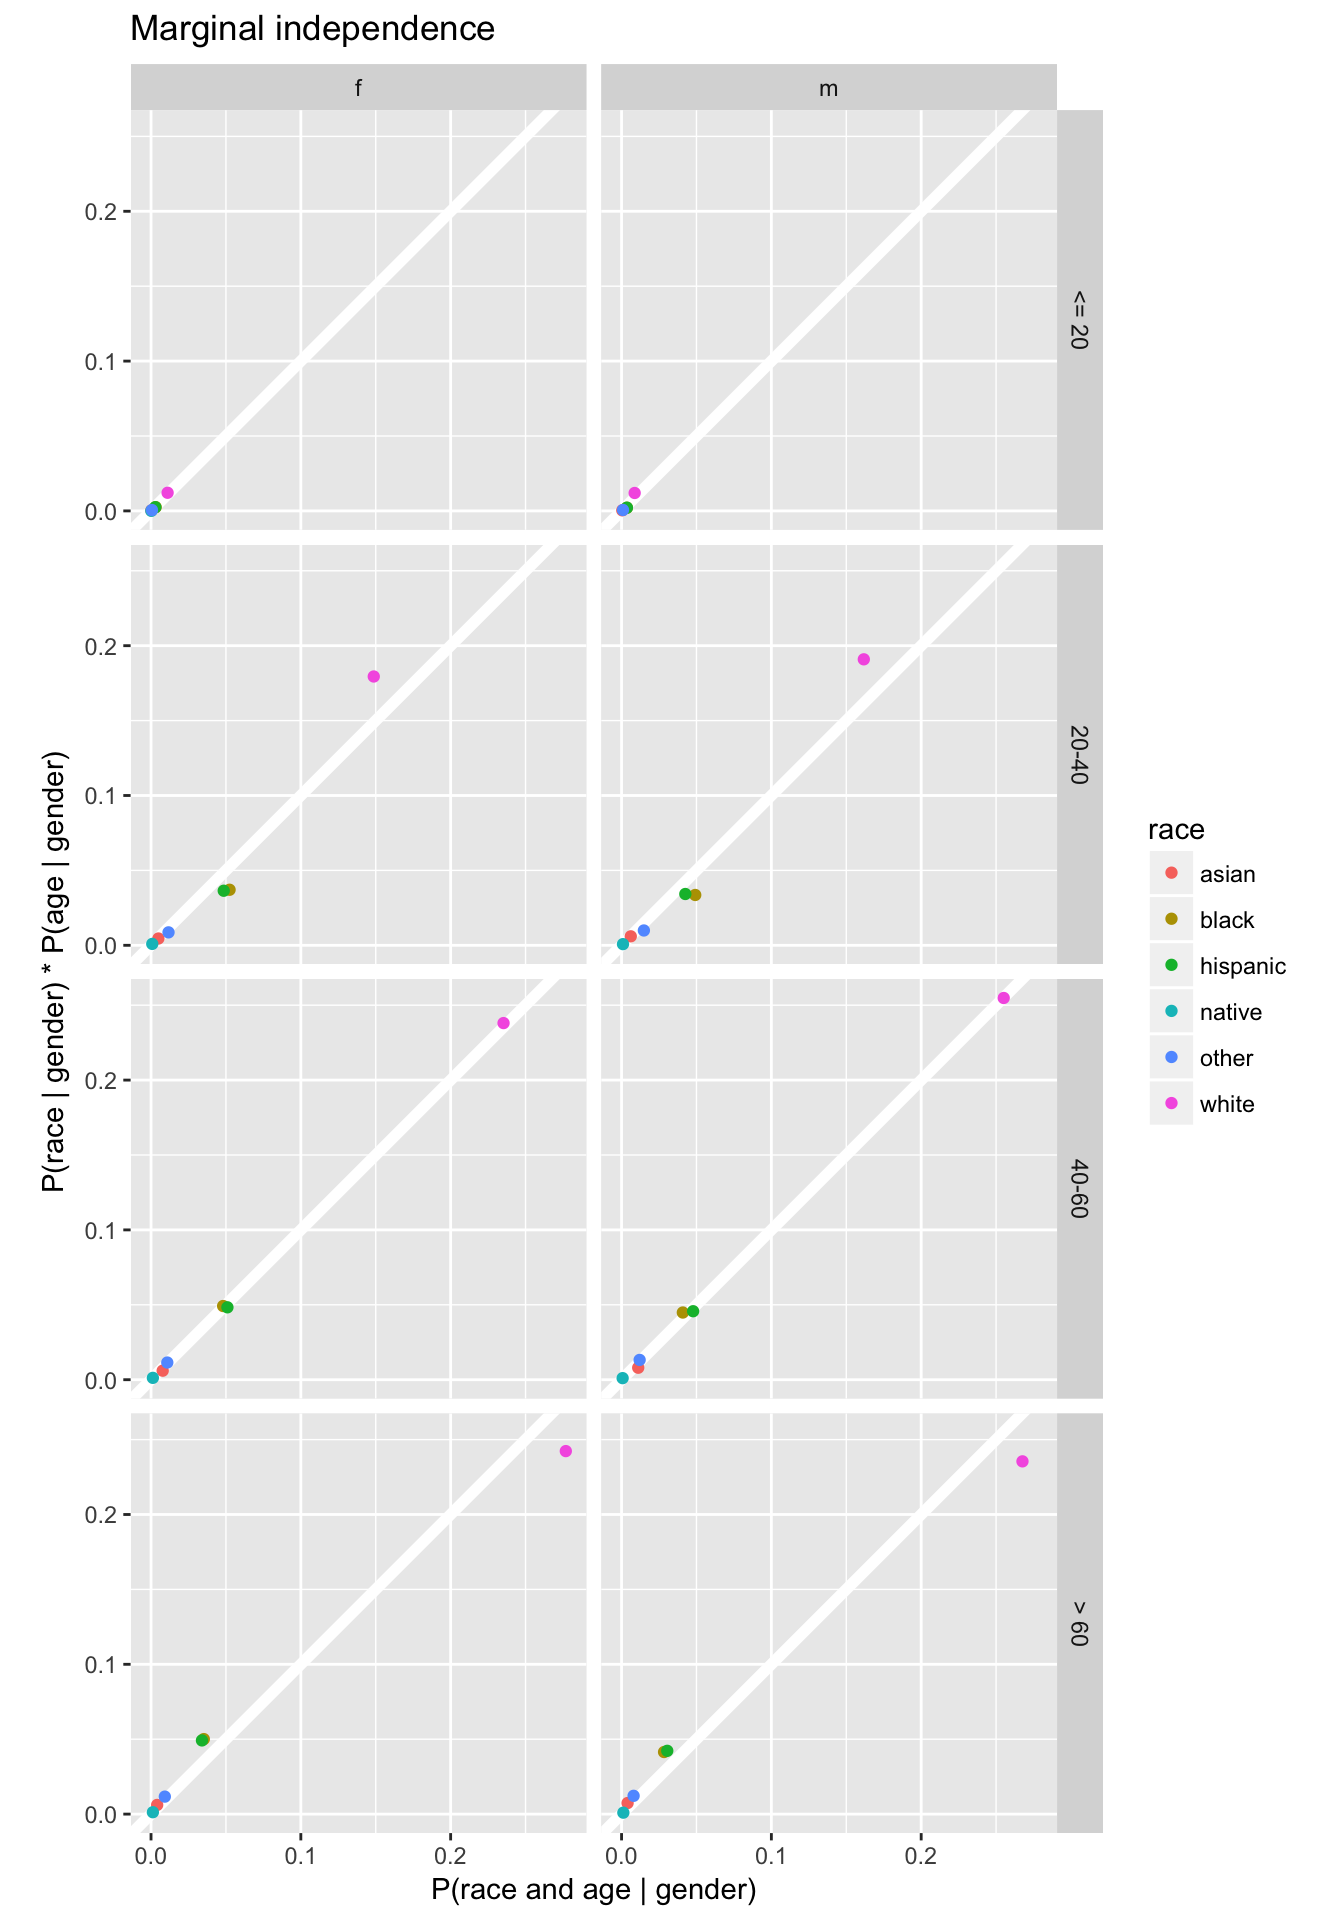
\includegraphics[width=0.7\linewidth]{measurement_files/figure-latex/unnamed-chunk-41-1} \end{center}

\begin{Shaded}
\begin{Highlighting}[]
\NormalTok{congress }\OperatorTok
\StringTok{  }\KeywordTok{ggplot}\NormalTok{(}\KeywordTok{aes}\NormalTok{(}\DataTypeTok{x =}\NormalTok{ dwnom1, }\DataTypeTok{y =}\NormalTok{ dwnom2, }\DataTypeTok{colour =}\NormalTok{ party)) }\OperatorTok{+}
\StringTok{  }\KeywordTok{geom_point}\NormalTok{() }\OperatorTok{+}
\StringTok{  }\KeywordTok{facet_wrap}\NormalTok{(}\OperatorTok{~}\StringTok{ }\NormalTok{congress) }\OperatorTok{+}
\StringTok{  }\KeywordTok{coord_fixed}\NormalTok{() }\OperatorTok{+}
\StringTok{  }\KeywordTok{scale_y_continuous}\NormalTok{(}\StringTok{"racial liberalism/conservatism"}\NormalTok{,}
                     \DataTypeTok{limits =} \KeywordTok{c}\NormalTok{(}\OperatorTok{-}\DecValTok{2}\NormalTok{, }\DecValTok{2}\NormalTok{)) }\OperatorTok{+}
\StringTok{  }\KeywordTok{scale_x_continuous}\NormalTok{(}\StringTok{"economic liberalism/conservatism"}\NormalTok{,}
                     \DataTypeTok{limits =} \KeywordTok{c}\NormalTok{(}\OperatorTok{-}\DecValTok{2}\NormalTok{, }\DecValTok{2}\NormalTok{)) }
  \CommentTok{#scale_colour_parties}
\end{Highlighting}
\end{Shaded}

\begin{center}\includegraphics[width=1\linewidth,height=1\textheight]{measurement_files/figure-latex/unnamed-chunk-42-1} \end{center}

\begin{Shaded}
\begin{Highlighting}[]
\NormalTok{congress }\OperatorTok
\StringTok{  }\KeywordTok{group_by}\NormalTok{(congress, party) }\OperatorTok
\StringTok{  }\KeywordTok{summarise}\NormalTok{(}\DataTypeTok{dwnom1 =} \KeywordTok{mean}\NormalTok{(dwnom1)) }\OperatorTok
\StringTok{  }\KeywordTok{filter}\NormalTok{(party }\OperatorTok\StringTok{ }\KeywordTok{c}\NormalTok{(}\StringTok{"Democrat"}\NormalTok{, }\StringTok{"Republican"}\NormalTok{)) }\OperatorTok
\StringTok{  }\KeywordTok{ggplot}\NormalTok{(}\KeywordTok{aes}\NormalTok{(}\DataTypeTok{x =}\NormalTok{ congress, }\DataTypeTok{y =}\NormalTok{ dwnom1,}
             \DataTypeTok{colour =} \KeywordTok{fct_reorder2}\NormalTok{(party, congress, dwnom1))) }\OperatorTok{+}
\StringTok{  }\KeywordTok{geom_line}\NormalTok{() }\OperatorTok{+}
\StringTok{  }\NormalTok{scale_colour_parties }\OperatorTok{+}
\StringTok{  }\KeywordTok{labs}\NormalTok{(}\DataTypeTok{y =} \StringTok{"DW-NOMINATE score (1st Dimension)"}\NormalTok{, }\DataTypeTok{x =} \StringTok{"Congress"}\NormalTok{,}
       \DataTypeTok{colour =} \StringTok{"Party"}\NormalTok{)}
\end{Highlighting}
\end{Shaded}

\begin{center}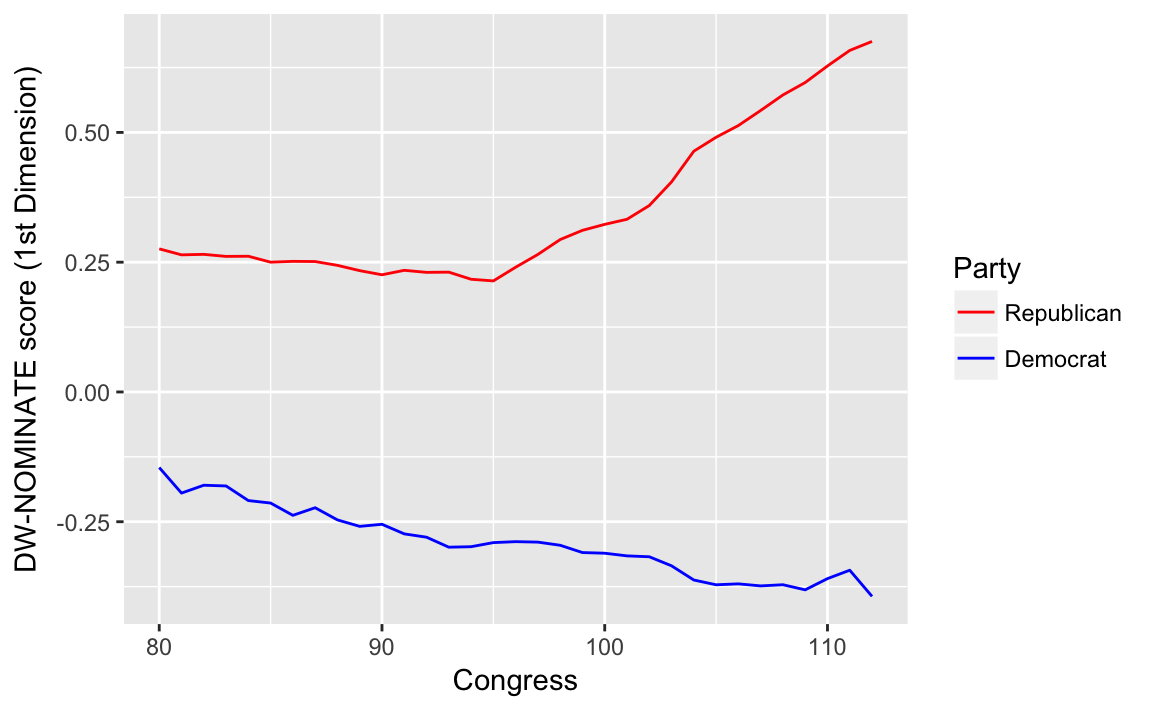
\includegraphics[width=0.7\linewidth]{measurement_files/figure-latex/unnamed-chunk-43-1} \end{center}

Alternatively, you can plot the mean DW-Nominate scores for each party
and congress over time. This plot uses color for parties and lets the
points and labels for the first and last congresses (80 and 112) to
convey progress through time.

\begin{Shaded}
\begin{Highlighting}[]
\NormalTok{party_means <-}
\StringTok{  }\NormalTok{congress }\OperatorTok
\StringTok{  }\KeywordTok{filter}\NormalTok{(party }\OperatorTok\StringTok{ }\KeywordTok{c}\NormalTok{(}\StringTok{"Democrat"}\NormalTok{, }\StringTok{"Republican"}\NormalTok{)) }\OperatorTok
\StringTok{  }\KeywordTok{group_by}\NormalTok{(party, congress) }\OperatorTok
\StringTok{  }\KeywordTok{summarise}\NormalTok{(}\DataTypeTok{dwnom1 =} \KeywordTok{mean}\NormalTok{(dwnom1),}
            \DataTypeTok{dwnom2 =} \KeywordTok{mean}\NormalTok{(dwnom2))}

\NormalTok{party_endpoints <-}
\StringTok{  }\NormalTok{party_means }\OperatorTok
\StringTok{  }\KeywordTok{filter}\NormalTok{(congress }\OperatorTok\StringTok{ }\KeywordTok{c}\NormalTok{(}\KeywordTok{min}\NormalTok{(congress), }\KeywordTok{max}\NormalTok{(congress))) }\OperatorTok
\StringTok{  }\KeywordTok{mutate}\NormalTok{(}\DataTypeTok{label =} \KeywordTok{str_c}\NormalTok{(party, congress, }\DataTypeTok{sep =} \StringTok{" - "}\NormalTok{))}

\KeywordTok{ggplot}\NormalTok{(party_means, }
         \KeywordTok{aes}\NormalTok{(}\DataTypeTok{x =}\NormalTok{ dwnom1, }\DataTypeTok{y =}\NormalTok{ dwnom2, }\DataTypeTok{color =}\NormalTok{ party,}
             \DataTypeTok{group =}\NormalTok{ party)) }\OperatorTok{+}
\StringTok{  }\KeywordTok{geom_point}\NormalTok{() }\OperatorTok{+}
\StringTok{  }\KeywordTok{geom_path}\NormalTok{() }\OperatorTok{+}
\StringTok{  }\NormalTok{ggrepel}\OperatorTok{::}\KeywordTok{geom_text_repel}\NormalTok{(}\DataTypeTok{data =}\NormalTok{ party_endpoints,}
                           \DataTypeTok{mapping =} \KeywordTok{aes}\NormalTok{(}\DataTypeTok{label =}\NormalTok{ congress),}
                           \DataTypeTok{color =} \StringTok{"black"}\NormalTok{) }\OperatorTok{+}
\StringTok{  }\KeywordTok{scale_y_continuous}\NormalTok{(}\StringTok{"racial liberalism/conservatism"}\NormalTok{) }\OperatorTok{+}
\StringTok{  }\KeywordTok{scale_x_continuous}\NormalTok{(}\StringTok{"economic liberalism/conservatism"}\NormalTok{) }\OperatorTok{+}
\StringTok{  }\NormalTok{scale_colour_parties}
\end{Highlighting}
\end{Shaded}

\begin{center}\includegraphics[width=0.7\linewidth]{measurement_files/figure-latex/unnamed-chunk-44-1} \end{center}

\hypertarget{correlation}{%
\subsection{Correlation}\label{correlation}}

Let's plot the Gini coefficient

\begin{Shaded}
\begin{Highlighting}[]
\KeywordTok{data}\NormalTok{(}\StringTok{"USGini"}\NormalTok{, }\DataTypeTok{package =} \StringTok{"qss"}\NormalTok{)}
\end{Highlighting}
\end{Shaded}

\begin{Shaded}
\begin{Highlighting}[]
\KeywordTok{ggplot}\NormalTok{(USGini, }\KeywordTok{aes}\NormalTok{(}\DataTypeTok{x =}\NormalTok{ year, }\DataTypeTok{y =}\NormalTok{ gini)) }\OperatorTok{+}
\StringTok{  }\KeywordTok{geom_point}\NormalTok{() }\OperatorTok{+}
\StringTok{  }\KeywordTok{geom_line}\NormalTok{() }\OperatorTok{+}
\StringTok{  }\KeywordTok{labs}\NormalTok{(}\DataTypeTok{x =} \StringTok{"Year"}\NormalTok{, }\DataTypeTok{y =} \StringTok{"Gini coefficient"}\NormalTok{) }\OperatorTok{+}
\StringTok{  }\KeywordTok{ggtitle}\NormalTok{(}\StringTok{"Income Inequality"}\NormalTok{)}
\end{Highlighting}
\end{Shaded}

\begin{center}\includegraphics[width=0.7\linewidth]{measurement_files/figure-latex/unnamed-chunk-46-1} \end{center}

To calculate a measure of party polarization take the code used in the
plot of Republican and Democratic party median ideal points and adapt it
to calculate the difference in the party medians:

\begin{Shaded}
\begin{Highlighting}[]
\NormalTok{party_polarization <-}
\StringTok{  }\NormalTok{congress }\OperatorTok
\StringTok{  }\KeywordTok{group_by}\NormalTok{(congress, party) }\OperatorTok
\StringTok{  }\KeywordTok{summarise}\NormalTok{(}\DataTypeTok{dwnom1 =} \KeywordTok{mean}\NormalTok{(dwnom1)) }\OperatorTok
\StringTok{  }\KeywordTok{filter}\NormalTok{(party }\OperatorTok\StringTok{ }\KeywordTok{c}\NormalTok{(}\StringTok{"Democrat"}\NormalTok{, }\StringTok{"Republican"}\NormalTok{)) }\OperatorTok
\StringTok{  }\KeywordTok{spread}\NormalTok{(party, dwnom1) }\OperatorTok
\StringTok{  }\KeywordTok{mutate}\NormalTok{(}\DataTypeTok{polarization =}\NormalTok{ Republican }\OperatorTok{-}\StringTok{ }\NormalTok{Democrat)}
\NormalTok{party_polarization}
\CommentTok{#> # A tibble: 33 x 4}
\CommentTok{#> # Groups:   congress [33]}
\CommentTok{#>   congress Democrat Republican polarization}
\CommentTok{#>      <int>    <dbl>      <dbl>        <dbl>}
\CommentTok{#> 1       80   -0.146      0.276        0.421}
\CommentTok{#> 2       81   -0.195      0.264        0.459}
\CommentTok{#> 3       82   -0.180      0.265        0.445}
\CommentTok{#> 4       83   -0.181      0.261        0.442}
\CommentTok{#> 5       84   -0.209      0.261        0.471}
\CommentTok{#> 6       85   -0.214      0.250        0.464}
\CommentTok{#> # ... with 27 more rows}
\end{Highlighting}
\end{Shaded}

\begin{Shaded}
\begin{Highlighting}[]
\KeywordTok{ggplot}\NormalTok{(party_polarization, }\KeywordTok{aes}\NormalTok{(}\DataTypeTok{x =}\NormalTok{ congress, }\DataTypeTok{y =}\NormalTok{ polarization)) }\OperatorTok{+}
\StringTok{  }\KeywordTok{geom_point}\NormalTok{() }\OperatorTok{+}
\StringTok{  }\KeywordTok{geom_line}\NormalTok{() }\OperatorTok{+}
\StringTok{  }\KeywordTok{ggtitle}\NormalTok{(}\StringTok{"Political Polarization"}\NormalTok{) }\OperatorTok{+}
\StringTok{  }\KeywordTok{labs}\NormalTok{(}\DataTypeTok{x =} \StringTok{"Year"}\NormalTok{, }\DataTypeTok{y =} \StringTok{"Republican median − Democratic median"}\NormalTok{)}
\CommentTok{#> Warning in grid.Call(C_stringMetric, as.graphicsAnnot(x$label)): font}
\CommentTok{#> metrics unknown for Unicode character U+2212}

\CommentTok{#> Warning in grid.Call(C_stringMetric, as.graphicsAnnot(x$label)): font}
\CommentTok{#> metrics unknown for Unicode character U+2212}
\CommentTok{#> Warning in grid.Call(C_stringMetric, as.graphicsAnnot(x$label)): conversion}
\CommentTok{#> failure on 'Republican median − Democratic median' in 'mbcsToSbcs': dot}
\CommentTok{#> substituted for <e2>}
\CommentTok{#> Warning in grid.Call(C_stringMetric, as.graphicsAnnot(x$label)): conversion}
\CommentTok{#> failure on 'Republican median − Democratic median' in 'mbcsToSbcs': dot}
\CommentTok{#> substituted for <88>}
\CommentTok{#> Warning in grid.Call(C_stringMetric, as.graphicsAnnot(x$label)): conversion}
\CommentTok{#> failure on 'Republican median − Democratic median' in 'mbcsToSbcs': dot}
\CommentTok{#> substituted for <92>}
\CommentTok{#> Warning in grid.Call(C_textBounds, as.graphicsAnnot(x$label), x$x, x}
\CommentTok{#> $y, : conversion failure on 'Republican median − Democratic median' in}
\CommentTok{#> 'mbcsToSbcs': dot substituted for <e2>}
\CommentTok{#> Warning in grid.Call(C_textBounds, as.graphicsAnnot(x$label), x$x, x}
\CommentTok{#> $y, : conversion failure on 'Republican median − Democratic median' in}
\CommentTok{#> 'mbcsToSbcs': dot substituted for <88>}
\CommentTok{#> Warning in grid.Call(C_textBounds, as.graphicsAnnot(x$label), x$x, x}
\CommentTok{#> $y, : conversion failure on 'Republican median − Democratic median' in}
\CommentTok{#> 'mbcsToSbcs': dot substituted for <92>}
\CommentTok{#> Warning in grid.Call(C_textBounds, as.graphicsAnnot(x$label), x$x, x}
\CommentTok{#> $y, : conversion failure on 'Republican median − Democratic median' in}
\CommentTok{#> 'mbcsToSbcs': dot substituted for <e2>}
\CommentTok{#> Warning in grid.Call(C_textBounds, as.graphicsAnnot(x$label), x$x, x}
\CommentTok{#> $y, : conversion failure on 'Republican median − Democratic median' in}
\CommentTok{#> 'mbcsToSbcs': dot substituted for <88>}
\CommentTok{#> Warning in grid.Call(C_textBounds, as.graphicsAnnot(x$label), x$x, x}
\CommentTok{#> $y, : conversion failure on 'Republican median − Democratic median' in}
\CommentTok{#> 'mbcsToSbcs': dot substituted for <92>}
\CommentTok{#> Warning in grid.Call(C_textBounds, as.graphicsAnnot(x$label), x$x, x}
\CommentTok{#> $y, : conversion failure on 'Republican median − Democratic median' in}
\CommentTok{#> 'mbcsToSbcs': dot substituted for <e2>}
\CommentTok{#> Warning in grid.Call(C_textBounds, as.graphicsAnnot(x$label), x$x, x}
\CommentTok{#> $y, : conversion failure on 'Republican median − Democratic median' in}
\CommentTok{#> 'mbcsToSbcs': dot substituted for <88>}
\CommentTok{#> Warning in grid.Call(C_textBounds, as.graphicsAnnot(x$label), x$x, x}
\CommentTok{#> $y, : conversion failure on 'Republican median − Democratic median' in}
\CommentTok{#> 'mbcsToSbcs': dot substituted for <92>}
\CommentTok{#> Warning in grid.Call(C_textBounds, as.graphicsAnnot(x$label), x$x, x}
\CommentTok{#> $y, : conversion failure on 'Republican median − Democratic median' in}
\CommentTok{#> 'mbcsToSbcs': dot substituted for <e2>}
\CommentTok{#> Warning in grid.Call(C_textBounds, as.graphicsAnnot(x$label), x$x, x}
\CommentTok{#> $y, : conversion failure on 'Republican median − Democratic median' in}
\CommentTok{#> 'mbcsToSbcs': dot substituted for <88>}
\CommentTok{#> Warning in grid.Call(C_textBounds, as.graphicsAnnot(x$label), x$x, x}
\CommentTok{#> $y, : conversion failure on 'Republican median − Democratic median' in}
\CommentTok{#> 'mbcsToSbcs': dot substituted for <92>}
\CommentTok{#> Warning in grid.Call(C_textBounds, as.graphicsAnnot(x$label), x$x, x}
\CommentTok{#> $y, : conversion failure on 'Republican median − Democratic median' in}
\CommentTok{#> 'mbcsToSbcs': dot substituted for <e2>}
\CommentTok{#> Warning in grid.Call(C_textBounds, as.graphicsAnnot(x$label), x$x, x}
\CommentTok{#> $y, : conversion failure on 'Republican median − Democratic median' in}
\CommentTok{#> 'mbcsToSbcs': dot substituted for <88>}
\CommentTok{#> Warning in grid.Call(C_textBounds, as.graphicsAnnot(x$label), x$x, x}
\CommentTok{#> $y, : conversion failure on 'Republican median − Democratic median' in}
\CommentTok{#> 'mbcsToSbcs': dot substituted for <92>}
\CommentTok{#> Warning in grid.Call(C_textBounds, as.graphicsAnnot(x$label), x$x, x}
\CommentTok{#> $y, : conversion failure on 'Republican median − Democratic median' in}
\CommentTok{#> 'mbcsToSbcs': dot substituted for <e2>}
\CommentTok{#> Warning in grid.Call(C_textBounds, as.graphicsAnnot(x$label), x$x, x}
\CommentTok{#> $y, : conversion failure on 'Republican median − Democratic median' in}
\CommentTok{#> 'mbcsToSbcs': dot substituted for <88>}
\CommentTok{#> Warning in grid.Call(C_textBounds, as.graphicsAnnot(x$label), x$x, x}
\CommentTok{#> $y, : conversion failure on 'Republican median − Democratic median' in}
\CommentTok{#> 'mbcsToSbcs': dot substituted for <92>}
\CommentTok{#> Warning in grid.Call(C_textBounds, as.graphicsAnnot(x$label), x$x, x}
\CommentTok{#> $y, : conversion failure on 'Republican median − Democratic median' in}
\CommentTok{#> 'mbcsToSbcs': dot substituted for <e2>}
\CommentTok{#> Warning in grid.Call(C_textBounds, as.graphicsAnnot(x$label), x$x, x}
\CommentTok{#> $y, : conversion failure on 'Republican median − Democratic median' in}
\CommentTok{#> 'mbcsToSbcs': dot substituted for <88>}
\CommentTok{#> Warning in grid.Call(C_textBounds, as.graphicsAnnot(x$label), x$x, x}
\CommentTok{#> $y, : conversion failure on 'Republican median − Democratic median' in}
\CommentTok{#> 'mbcsToSbcs': dot substituted for <92>}
\CommentTok{#> Warning in grid.Call.graphics(C_text, as.graphicsAnnot(x$label), x$x, x}
\CommentTok{#> $y, : conversion failure on 'Republican median − Democratic median' in}
\CommentTok{#> 'mbcsToSbcs': dot substituted for <e2>}
\CommentTok{#> Warning in grid.Call.graphics(C_text, as.graphicsAnnot(x$label), x$x, x}
\CommentTok{#> $y, : conversion failure on 'Republican median − Democratic median' in}
\CommentTok{#> 'mbcsToSbcs': dot substituted for <88>}
\CommentTok{#> Warning in grid.Call.graphics(C_text, as.graphicsAnnot(x$label), x$x, x}
\CommentTok{#> $y, : conversion failure on 'Republican median − Democratic median' in}
\CommentTok{#> 'mbcsToSbcs': dot substituted for <92>}
\end{Highlighting}
\end{Shaded}

\begin{center}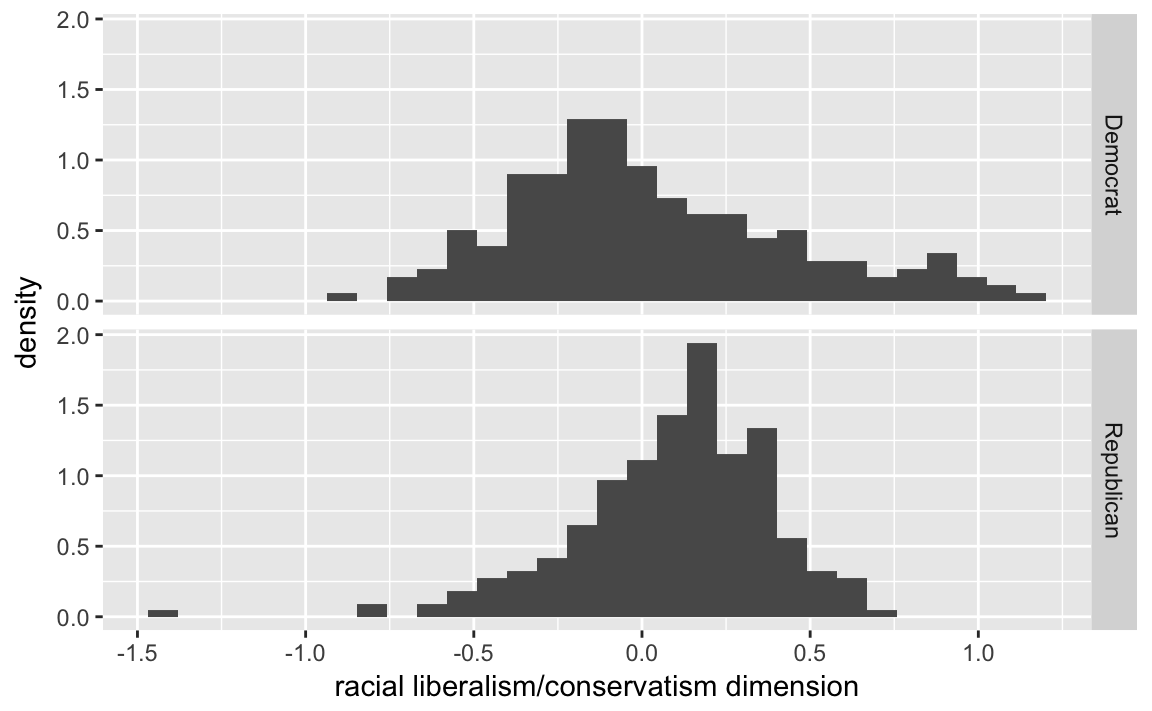
\includegraphics[width=0.7\linewidth]{measurement_files/figure-latex/unnamed-chunk-48-1} \end{center}

\hypertarget{quantile-quantile-plot}{%
\subsection{Quantile-Quantile Plot}\label{quantile-quantile-plot}}

\begin{Shaded}
\begin{Highlighting}[]
\NormalTok{congress }\OperatorTok
\StringTok{  }\KeywordTok{filter}\NormalTok{(congress }\OperatorTok{==}\StringTok{ }\DecValTok{112}\NormalTok{, party }\OperatorTok\StringTok{ }\KeywordTok{c}\NormalTok{(}\StringTok{"Republican"}\NormalTok{, }\StringTok{"Democrat"}\NormalTok{)) }\OperatorTok
\StringTok{  }\KeywordTok{ggplot}\NormalTok{(}\KeywordTok{aes}\NormalTok{(}\DataTypeTok{x =}\NormalTok{ dwnom2, }\DataTypeTok{y =}\NormalTok{ ..density..)) }\OperatorTok{+}
\StringTok{  }\KeywordTok{geom_histogram}\NormalTok{(}\DataTypeTok{binwidth =} \FloatTok{.2}\NormalTok{) }\OperatorTok{+}
\StringTok{  }\KeywordTok{facet_grid}\NormalTok{(party }\OperatorTok{~}\StringTok{ }\NormalTok{.) }\OperatorTok{+}
\StringTok{  }\KeywordTok{labs}\NormalTok{(}\DataTypeTok{x =} \StringTok{"racial liberalism/conservatism dimension"}\NormalTok{)}
\end{Highlighting}
\end{Shaded}

\begin{center}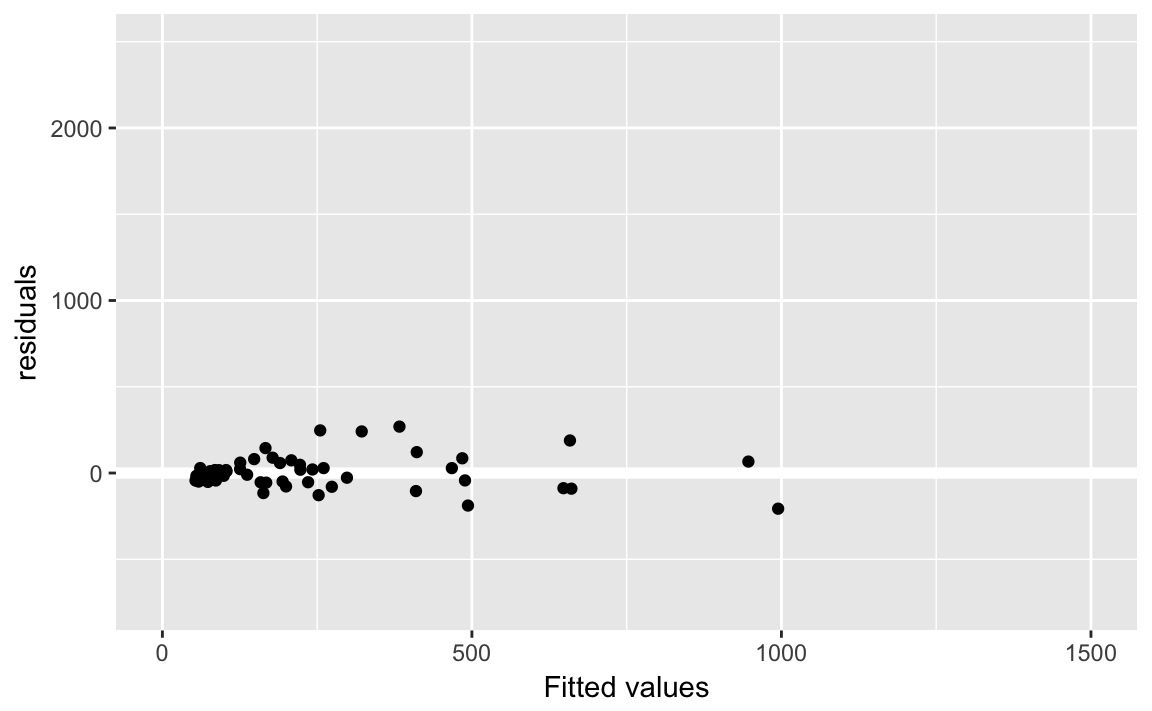
\includegraphics[width=0.7\linewidth]{measurement_files/figure-latex/unnamed-chunk-49-1} \end{center}

The package \emph{ggplot2} includes a function \texttt{stat\_qq} which
can be used to create qq-plots but it is more suited to comparing a
sample distribution with a theoretical distribution, usually the normal
one. However, we can calculate one by hand, which may give more insight
into exactly what the qq-plot is doing.

\begin{Shaded}
\begin{Highlighting}[]
\NormalTok{party_qtiles <-}\StringTok{ }\KeywordTok{tibble}\NormalTok{(}
  \DataTypeTok{probs =} \KeywordTok{seq}\NormalTok{(}\DecValTok{0}\NormalTok{, }\DecValTok{1}\NormalTok{, }\DataTypeTok{by =} \FloatTok{0.01}\NormalTok{),}
  \DataTypeTok{Democrat =} \KeywordTok{quantile}\NormalTok{(}\KeywordTok{filter}\NormalTok{(congress, congress }\OperatorTok{==}\StringTok{ }\DecValTok{112}\NormalTok{,}
\NormalTok{                             party }\OperatorTok{==}\StringTok{ "Democrat"}\NormalTok{)}\OperatorTok{$}\NormalTok{dwnom2,}
         \DataTypeTok{probs =}\NormalTok{ probs),}
  \DataTypeTok{Republican =} \KeywordTok{quantile}\NormalTok{(}\KeywordTok{filter}\NormalTok{(congress, congress }\OperatorTok{==}\StringTok{ }\DecValTok{112}\NormalTok{,}
\NormalTok{                               party }\OperatorTok{==}\StringTok{ "Republican"}\NormalTok{)}\OperatorTok{$}\NormalTok{dwnom2,}
         \DataTypeTok{probs =}\NormalTok{ probs)}
\NormalTok{)}
\NormalTok{party_qtiles}
\CommentTok{#> # A tibble: 101 x 3}
\CommentTok{#>    probs Democrat Republican}
\CommentTok{#>    <dbl>    <dbl>      <dbl>}
\CommentTok{#> 1 0.       -0.925     -1.38 }
\CommentTok{#> 2 0.0100   -0.672     -0.720}
\CommentTok{#> 3 0.0200   -0.619     -0.566}
\CommentTok{#> 4 0.0300   -0.593     -0.526}
\CommentTok{#> 5 0.0400   -0.567     -0.468}
\CommentTok{#> 6 0.0500   -0.560     -0.436}
\CommentTok{#> # ... with 95 more rows}
\end{Highlighting}
\end{Shaded}

The plot looks different than the one in the text since the x- and
y-scales are in the original values instead of z-scores (see the next
section).

\begin{Shaded}
\begin{Highlighting}[]
\NormalTok{party_qtiles }\OperatorTok
\StringTok{  }\KeywordTok{ggplot}\NormalTok{(}\KeywordTok{aes}\NormalTok{(}\DataTypeTok{x =}\NormalTok{ Democrat, }\DataTypeTok{y =}\NormalTok{ Republican)) }\OperatorTok{+}
\StringTok{  }\KeywordTok{geom_point}\NormalTok{() }\OperatorTok{+}
\StringTok{  }\KeywordTok{geom_abline}\NormalTok{() }\OperatorTok{+}
\StringTok{  }\KeywordTok{coord_fixed}\NormalTok{()}
\end{Highlighting}
\end{Shaded}

\begin{center}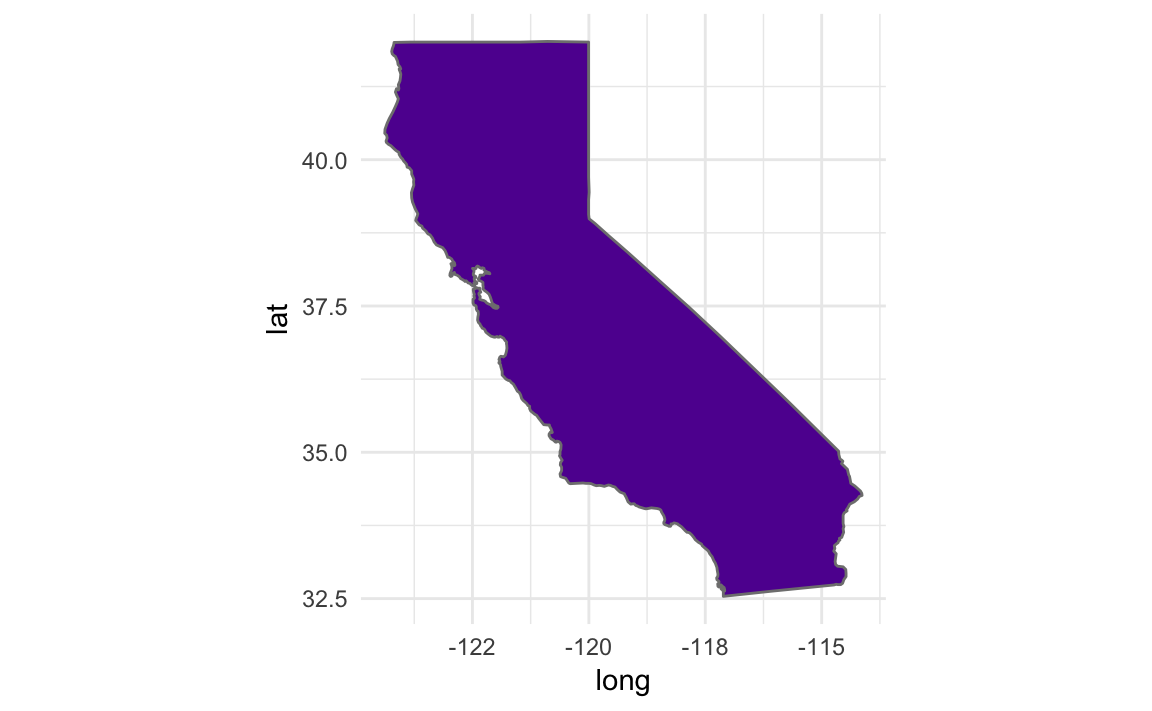
\includegraphics[width=0.7\linewidth]{measurement_files/figure-latex/unnamed-chunk-51-1} \end{center}

\hypertarget{clustering}{%
\section{Clustering}\label{clustering}}

\hypertarget{matrices}{%
\subsection{Matrices}\label{matrices}}

While matrices are great for numerical computations, such as when you
are implementing algorithms, generally keeping data in data frames is
more convenient for data wrangling.

See \href{http://r4ds.had.co.nz/}{R for Data Science} chapter
\href{http://r4ds.had.co.nz/vectors.html}{Vectors}.

\hypertarget{lists}{%
\subsection{Lists}\label{lists}}

See \href{http://r4ds.had.co.nz/}{R for Data Science} chapters
\href{http://r4ds.had.co.nz/vectors.html}{Vectors} and
\href{http://r4ds.had.co.nz/iteration.html}{Iteration}, as well as the
\href{https://cran.r-project.org/package=purrr}{purrr} package for more
powerful methods of computing on lists.

\hypertarget{k-means-algorithms}{%
\subsection{k-means algorithms}\label{k-means-algorithms}}

Calculate the clusters by the 80th and 112th congresses:

\begin{Shaded}
\begin{Highlighting}[]
\NormalTok{k80two.out <-}
\StringTok{  }\KeywordTok{kmeans}\NormalTok{(}\KeywordTok{select}\NormalTok{(}\KeywordTok{filter}\NormalTok{(congress, congress }\OperatorTok{==}\StringTok{ }\DecValTok{80}\NormalTok{),}
\NormalTok{                       dwnom1, dwnom2),}
              \DataTypeTok{centers =} \DecValTok{2}\NormalTok{, }\DataTypeTok{nstart =} \DecValTok{5}\NormalTok{)}
\end{Highlighting}
\end{Shaded}

Add the cluster ids to data sets:

\begin{Shaded}
\begin{Highlighting}[]
\NormalTok{congress80 <-}
\StringTok{  }\NormalTok{congress }\OperatorTok
\StringTok{  }\KeywordTok{filter}\NormalTok{(congress }\OperatorTok{==}\StringTok{ }\DecValTok{80}\NormalTok{) }\OperatorTok
\StringTok{  }\KeywordTok{mutate}\NormalTok{(}\DataTypeTok{cluster2 =} \KeywordTok{factor}\NormalTok{(k80two.out}\OperatorTok{$}\NormalTok{cluster))}
\end{Highlighting}
\end{Shaded}

We will also create a data sets with the cluster centroids. These are in
the \texttt{centers} element of the cluster object.

\begin{Shaded}
\begin{Highlighting}[]
\NormalTok{k80two.out}\OperatorTok{$}\NormalTok{centers}
\CommentTok{#>    dwnom1 dwnom2}
\CommentTok{#> 1 -0.0484  0.783}
\CommentTok{#> 2  0.1468 -0.339}
\end{Highlighting}
\end{Shaded}

To make it easier to use with
\href{https://cran.r-project.org/package=ggplot2}{ggplot2}, we need to
convert this to a data frame. The
\href{https://www.rdocumentation.org/packages/broom/topics/tidy}{tidy}
function from the \href{https://cran.r-project.org/package=broom}{broom}
package:

\begin{Shaded}
\begin{Highlighting}[]
\NormalTok{k80two.clusters <-}\StringTok{ }\KeywordTok{tidy}\NormalTok{(k80two.out)}
\NormalTok{k80two.clusters}
\CommentTok{#>        x1     x2 size withinss cluster}
\CommentTok{#> 1 -0.0484  0.783  135     10.9       1}
\CommentTok{#> 2  0.1468 -0.339  311     54.9       2}
\end{Highlighting}
\end{Shaded}

Plot the ideal points and clusters:

\begin{Shaded}
\begin{Highlighting}[]
\KeywordTok{ggplot}\NormalTok{() }\OperatorTok{+}
\StringTok{  }\KeywordTok{geom_point}\NormalTok{(}\DataTypeTok{data =}\NormalTok{ congress80,}
             \KeywordTok{aes}\NormalTok{(}\DataTypeTok{x =}\NormalTok{ dwnom1, }\DataTypeTok{y =}\NormalTok{ dwnom2, }\DataTypeTok{colour =}\NormalTok{ cluster2)) }\OperatorTok{+}
\StringTok{  }\KeywordTok{geom_point}\NormalTok{(}\DataTypeTok{data =}\NormalTok{ k80two.clusters, }\DataTypeTok{mapping =} \KeywordTok{aes}\NormalTok{(}\DataTypeTok{x =}\NormalTok{ x1, }\DataTypeTok{y =}\NormalTok{ x2))}
\end{Highlighting}
\end{Shaded}

\begin{center}\includegraphics[width=0.7\linewidth]{measurement_files/figure-latex/unnamed-chunk-56-1} \end{center}

\begin{Shaded}
\begin{Highlighting}[]
\NormalTok{congress80 }\OperatorTok
\StringTok{  }\KeywordTok{group_by}\NormalTok{(party, cluster2) }\OperatorTok
\StringTok{  }\KeywordTok{count}\NormalTok{()}
\CommentTok{#> # A tibble: 5 x 3}
\CommentTok{#> # Groups:   party, cluster2 [5]}
\CommentTok{#>   party      cluster2     n}
\CommentTok{#>   <chr>      <fct>    <int>}
\CommentTok{#> 1 Democrat   1          132}
\CommentTok{#> 2 Democrat   2           62}
\CommentTok{#> 3 Other      2            2}
\CommentTok{#> 4 Republican 1            3}
\CommentTok{#> 5 Republican 2          247}
\end{Highlighting}
\end{Shaded}

And now we can repeat these steps for the 112th congress:

\begin{Shaded}
\begin{Highlighting}[]
\NormalTok{k112two.out <-}
\StringTok{  }\KeywordTok{kmeans}\NormalTok{(}\KeywordTok{select}\NormalTok{(}\KeywordTok{filter}\NormalTok{(congress, congress }\OperatorTok{==}\StringTok{ }\DecValTok{112}\NormalTok{),}
\NormalTok{                dwnom1, dwnom2),}
         \DataTypeTok{centers =} \DecValTok{2}\NormalTok{, }\DataTypeTok{nstart =} \DecValTok{5}\NormalTok{)}
\NormalTok{congress112 <-}
\StringTok{  }\KeywordTok{filter}\NormalTok{(congress, congress }\OperatorTok{==}\StringTok{ }\DecValTok{112}\NormalTok{) }\OperatorTok
\StringTok{  }\KeywordTok{mutate}\NormalTok{(}\DataTypeTok{cluster2 =} \KeywordTok{factor}\NormalTok{(k112two.out}\OperatorTok{$}\NormalTok{cluster))}
\NormalTok{k112two.clusters <-}\StringTok{ }\KeywordTok{tidy}\NormalTok{(k112two.out)}
\KeywordTok{ggplot}\NormalTok{() }\OperatorTok{+}
\StringTok{  }\KeywordTok{geom_point}\NormalTok{(}\DataTypeTok{data =}\NormalTok{ congress112,}
             \DataTypeTok{mapping =} \KeywordTok{aes}\NormalTok{(}\DataTypeTok{x =}\NormalTok{ dwnom1, }\DataTypeTok{y =}\NormalTok{ dwnom2, }\DataTypeTok{colour =}\NormalTok{ cluster2)) }\OperatorTok{+}
\StringTok{  }\KeywordTok{geom_point}\NormalTok{(}\DataTypeTok{data =}\NormalTok{ k112two.clusters,}
             \DataTypeTok{mapping =} \KeywordTok{aes}\NormalTok{(}\DataTypeTok{x =}\NormalTok{ x1, }\DataTypeTok{y =}\NormalTok{ x2))}
\end{Highlighting}
\end{Shaded}

\begin{center}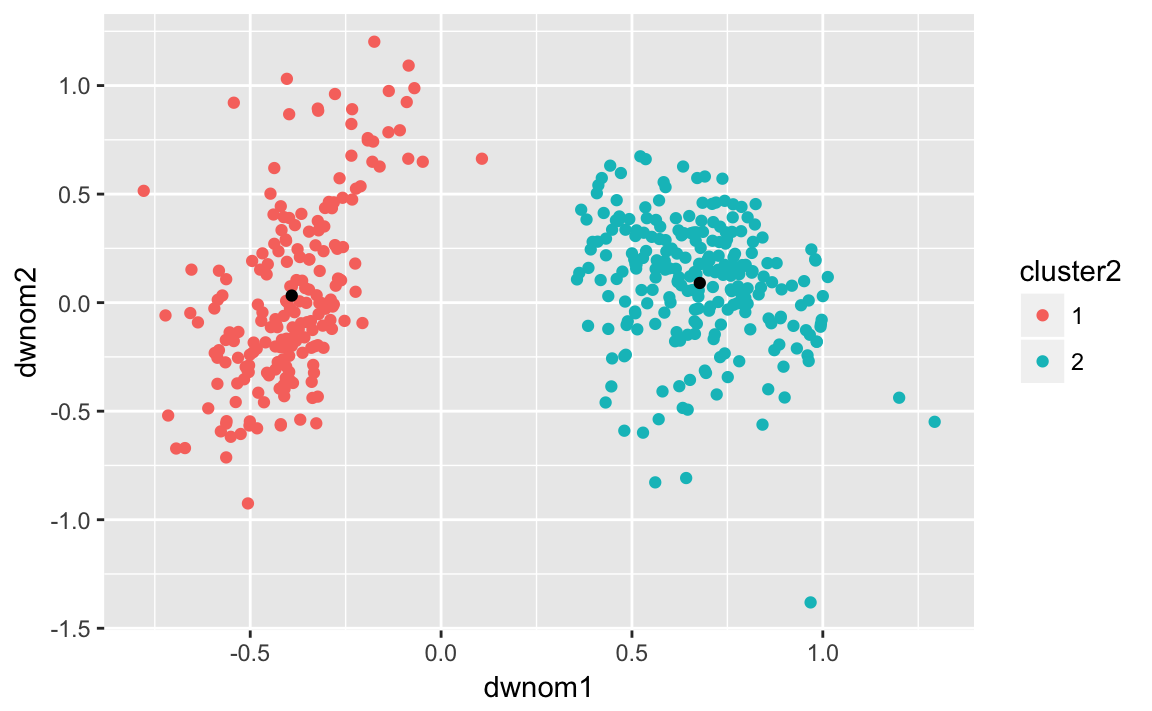
\includegraphics[width=0.7\linewidth]{measurement_files/figure-latex/unnamed-chunk-58-1} \end{center}

Number of observations from each party in each cluster:

\begin{Shaded}
\begin{Highlighting}[]
\NormalTok{congress112 }\OperatorTok
\StringTok{  }\KeywordTok{group_by}\NormalTok{(party, cluster2) }\OperatorTok
\StringTok{  }\KeywordTok{count}\NormalTok{()}
\CommentTok{#> # A tibble: 3 x 3}
\CommentTok{#> # Groups:   party, cluster2 [3]}
\CommentTok{#>   party      cluster2     n}
\CommentTok{#>   <chr>      <fct>    <int>}
\CommentTok{#> 1 Democrat   1          200}
\CommentTok{#> 2 Republican 1            1}
\CommentTok{#> 3 Republican 2          242}
\end{Highlighting}
\end{Shaded}

Now repeat the same with four clusters on the 80th congress:

\begin{Shaded}
\begin{Highlighting}[]
\NormalTok{k80four.out <-}
\StringTok{  }\KeywordTok{kmeans}\NormalTok{(}\KeywordTok{select}\NormalTok{(}\KeywordTok{filter}\NormalTok{(congress, congress }\OperatorTok{==}\StringTok{ }\DecValTok{80}\NormalTok{),}
\NormalTok{                dwnom1, dwnom2),}
         \DataTypeTok{centers =} \DecValTok{4}\NormalTok{, }\DataTypeTok{nstart =} \DecValTok{5}\NormalTok{)}
\NormalTok{congress80 <-}
\StringTok{  }\KeywordTok{filter}\NormalTok{(congress, congress }\OperatorTok{==}\StringTok{ }\DecValTok{80}\NormalTok{) }\OperatorTok
\StringTok{  }\KeywordTok{mutate}\NormalTok{(}\DataTypeTok{cluster2 =} \KeywordTok{factor}\NormalTok{(k80four.out}\OperatorTok{$}\NormalTok{cluster))}
\NormalTok{k80four.clusters <-}\StringTok{ }\KeywordTok{tidy}\NormalTok{(k80four.out)}
\KeywordTok{ggplot}\NormalTok{() }\OperatorTok{+}
\StringTok{  }\KeywordTok{geom_point}\NormalTok{(}\DataTypeTok{data =}\NormalTok{ congress80,}
             \DataTypeTok{mapping =} \KeywordTok{aes}\NormalTok{(}\DataTypeTok{x =}\NormalTok{ dwnom1, }\DataTypeTok{y =}\NormalTok{ dwnom2, }\DataTypeTok{colour =}\NormalTok{ cluster2)) }\OperatorTok{+}
\StringTok{  }\KeywordTok{geom_point}\NormalTok{(}\DataTypeTok{data =}\NormalTok{ k80four.clusters,}
             \DataTypeTok{mapping =} \KeywordTok{aes}\NormalTok{(}\DataTypeTok{x =}\NormalTok{ x1, }\DataTypeTok{y =}\NormalTok{ x2), }\DataTypeTok{size =} \DecValTok{3}\NormalTok{)}
\end{Highlighting}
\end{Shaded}

\begin{center}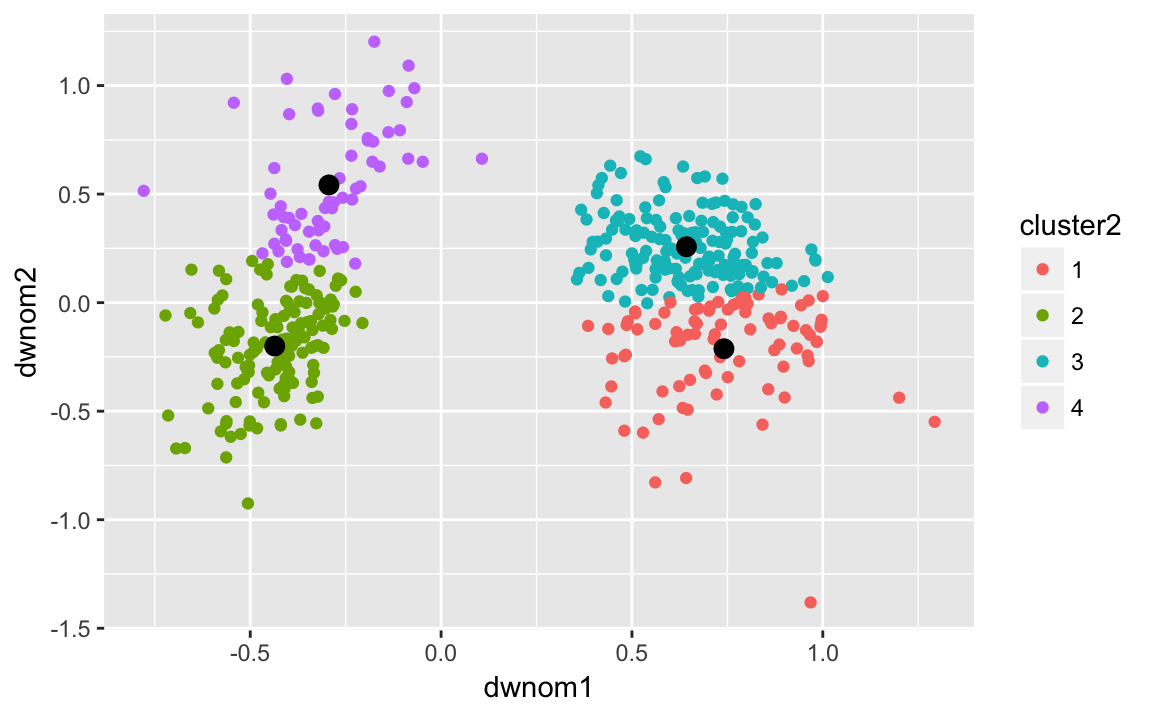
\includegraphics[width=0.7\linewidth]{measurement_files/figure-latex/unnamed-chunk-60-1} \end{center}

and on the 112th congress:

\begin{Shaded}
\begin{Highlighting}[]
\NormalTok{k112four.out <-}
\StringTok{  }\KeywordTok{kmeans}\NormalTok{(}\KeywordTok{select}\NormalTok{(}\KeywordTok{filter}\NormalTok{(congress, congress }\OperatorTok{==}\StringTok{ }\DecValTok{112}\NormalTok{),}
\NormalTok{                dwnom1, dwnom2),}
         \DataTypeTok{centers =} \DecValTok{4}\NormalTok{, }\DataTypeTok{nstart =} \DecValTok{5}\NormalTok{)}
\NormalTok{congress112 <-}
\StringTok{  }\KeywordTok{filter}\NormalTok{(congress, congress }\OperatorTok{==}\StringTok{ }\DecValTok{112}\NormalTok{) }\OperatorTok
\StringTok{  }\KeywordTok{mutate}\NormalTok{(}\DataTypeTok{cluster2 =} \KeywordTok{factor}\NormalTok{(k112four.out}\OperatorTok{$}\NormalTok{cluster))}
\NormalTok{k112four.clusters <-}\StringTok{ }\KeywordTok{tidy}\NormalTok{(k112four.out)}
\KeywordTok{ggplot}\NormalTok{() }\OperatorTok{+}
\StringTok{  }\KeywordTok{geom_point}\NormalTok{(}\DataTypeTok{data =}\NormalTok{ congress112,}
             \DataTypeTok{mapping =} \KeywordTok{aes}\NormalTok{(}\DataTypeTok{x =}\NormalTok{ dwnom1, }\DataTypeTok{y =}\NormalTok{ dwnom2, }\DataTypeTok{colour =}\NormalTok{ cluster2)) }\OperatorTok{+}
\StringTok{  }\KeywordTok{geom_point}\NormalTok{(}\DataTypeTok{data =}\NormalTok{ k112four.clusters,}
             \DataTypeTok{mapping =} \KeywordTok{aes}\NormalTok{(}\DataTypeTok{x =}\NormalTok{ x1, }\DataTypeTok{y =}\NormalTok{ x2), }\DataTypeTok{size =} \DecValTok{3}\NormalTok{)}
\end{Highlighting}
\end{Shaded}

\begin{center}\includegraphics[width=0.7\linewidth]{measurement_files/figure-latex/unnamed-chunk-61-1} \end{center}

\hypertarget{prediction}{%
\chapter{Prediction}\label{prediction}}

\hypertarget{prerequisites-3}{%
\section*{Prerequisites}\label{prerequisites-3}}
\addcontentsline{toc}{section}{Prerequisites}

\begin{Shaded}
\begin{Highlighting}[]
\KeywordTok{library}\NormalTok{(}\StringTok{"tidyverse"}\NormalTok{)}
\KeywordTok{library}\NormalTok{(}\StringTok{"lubridate"}\NormalTok{)}
\KeywordTok{library}\NormalTok{(}\StringTok{"stringr"}\NormalTok{)}
\KeywordTok{library}\NormalTok{(}\StringTok{"forcats"}\NormalTok{)}
\end{Highlighting}
\end{Shaded}

The packages \href{https://cran.r-project.org/package=modelr}{modelr}
and \href{https://cran.r-project.org/package=broom}{broom} are used to
wrangle the results of linear regressions,

\begin{Shaded}
\begin{Highlighting}[]
\KeywordTok{library}\NormalTok{(}\StringTok{"broom"}\NormalTok{)}
\KeywordTok{library}\NormalTok{(}\StringTok{"modelr"}\NormalTok{)}
\end{Highlighting}
\end{Shaded}

\hypertarget{predicting-election-outcomes}{%
\section{Predicting Election
Outcomes}\label{predicting-election-outcomes}}

\hypertarget{loops-in-r}{%
\subsection{Loops in R}\label{loops-in-r}}

RStudio provides many features to help debugging, which will be useful
in for loops and function: see
\href{https://support.rstudio.com/hc/en-us/articles/205612627-Debugging-with-RStudio}{this}
article for an example.

\begin{Shaded}
\begin{Highlighting}[]
\NormalTok{values <-}\StringTok{ }\KeywordTok{c}\NormalTok{(}\DecValTok{2}\NormalTok{, }\DecValTok{3}\NormalTok{, }\DecValTok{6}\NormalTok{)}
\NormalTok{n <-}\StringTok{ }\KeywordTok{length}\NormalTok{(values)}
\NormalTok{results <-}\StringTok{ }\KeywordTok{rep}\NormalTok{(}\OtherTok{NA}\NormalTok{, n)}
\ControlFlowTok{for}\NormalTok{ (i }\ControlFlowTok{in} \DecValTok{1}\OperatorTok{:}\NormalTok{n) \{}
\NormalTok{  results[i] <-}\StringTok{ }\NormalTok{values[i] }\OperatorTok{*}\StringTok{ }\DecValTok{2}
  \KeywordTok{cat}\NormalTok{(values[i], }\StringTok{"times 2 is equal to"}\NormalTok{, results[i], }\StringTok{"}\CharTok{\textbackslash{}n}\StringTok{"}\NormalTok{)}
\NormalTok{\}}
\CommentTok{#> 2 times 2 is equal to 4 }
\CommentTok{#> 3 times 2 is equal to 6 }
\CommentTok{#> 6 times 2 is equal to 12}
\end{Highlighting}
\end{Shaded}

Note that the above code uses the for loop for pedagogical purposes
only, this could have simply been written

\begin{Shaded}
\begin{Highlighting}[]
\NormalTok{results <-}\StringTok{ }\NormalTok{values }\OperatorTok{*}\StringTok{ }\DecValTok{2}
\NormalTok{results}
\CommentTok{#> [1]  4  6 12}
\end{Highlighting}
\end{Shaded}

In general, avoid using for loops when there is a \emph{vectorized}
function.

But sticking with the for loop, there are several things that could be
improved.

Avoid using the idiom \texttt{1:n} in for loops. To see why, look what
happens when values are empty:

\begin{Shaded}
\begin{Highlighting}[]
\NormalTok{values <-}\StringTok{ }\KeywordTok{c}\NormalTok{()}
\NormalTok{n <-}\StringTok{ }\KeywordTok{length}\NormalTok{(values)}
\NormalTok{results <-}\StringTok{ }\KeywordTok{rep}\NormalTok{(}\OtherTok{NA}\NormalTok{, n)}
\ControlFlowTok{for}\NormalTok{ (i }\ControlFlowTok{in} \DecValTok{1}\OperatorTok{:}\NormalTok{n) \{}
  \KeywordTok{cat}\NormalTok{(}\StringTok{"i = "}\NormalTok{, i, }\StringTok{"}\CharTok{\textbackslash{}n}\StringTok{"}\NormalTok{)}
\NormalTok{  results[i] <-}\StringTok{ }\NormalTok{values[i] }\OperatorTok{*}\StringTok{ }\DecValTok{2}
  \KeywordTok{cat}\NormalTok{(values[i], }\StringTok{"times 2 is equal to"}\NormalTok{, results[i], }\StringTok{"}\CharTok{\textbackslash{}n}\StringTok{"}\NormalTok{)}
\NormalTok{\}}
\CommentTok{#> i =  1 }
\CommentTok{#>  times 2 is equal to NA }
\CommentTok{#> i =  0 }
\CommentTok{#>  times 2 is equal to}
\end{Highlighting}
\end{Shaded}

Instead of not running a loop, as you would expect, it runs two loops,
where \texttt{i\ =\ 1}, then \texttt{i\ =\ 0}. This edge case occurs
more than you may think, especially if you are writing functions where
you don't know the length of the vector is \emph{ex ante}.

The way to avoid this is to use either
\texttt{rdoc("base",\ "seq\_len")} or
\texttt{rdoc("base",\ "seq\_along")}, which will handle 0-length vectors
correctly.

\begin{Shaded}
\begin{Highlighting}[]
\NormalTok{values <-}\StringTok{ }\KeywordTok{c}\NormalTok{()}
\NormalTok{n <-}\StringTok{ }\KeywordTok{length}\NormalTok{(values)}
\NormalTok{results <-}\StringTok{ }\KeywordTok{rep}\NormalTok{(}\OtherTok{NA}\NormalTok{, n)}
\ControlFlowTok{for}\NormalTok{ (i }\ControlFlowTok{in} \KeywordTok{seq_along}\NormalTok{(values)) \{}
\NormalTok{  results[i] <-}\StringTok{ }\NormalTok{values[i] }\OperatorTok{*}\StringTok{ }\DecValTok{2}
\NormalTok{\}}
\KeywordTok{print}\NormalTok{(results)}
\CommentTok{#> logical(0)}
\end{Highlighting}
\end{Shaded}

or

\begin{Shaded}
\begin{Highlighting}[]
\NormalTok{values <-}\StringTok{ }\KeywordTok{c}\NormalTok{()}
\NormalTok{n <-}\StringTok{ }\KeywordTok{length}\NormalTok{(values)}
\NormalTok{results <-}\StringTok{ }\KeywordTok{rep}\NormalTok{(}\OtherTok{NA}\NormalTok{, n)}
\ControlFlowTok{for}\NormalTok{ (i }\ControlFlowTok{in} \KeywordTok{seq_len}\NormalTok{(n)) \{}
\NormalTok{  results[i] <-}\StringTok{ }\NormalTok{values[i] }\OperatorTok{*}\StringTok{ }\DecValTok{2}
\NormalTok{\}}
\KeywordTok{print}\NormalTok{(results)}
\CommentTok{#> logical(0)}
\end{Highlighting}
\end{Shaded}

Also, note that the the result is \texttt{logical(0)}. That's because
the \texttt{NA} missing value has class
\href{http://r4ds.had.co.nz/vectors.html\#missing-values-4}{logical},
and thus \texttt{rep(NA,\ ...)} returns a logical vector. It is better
style to initialize the vector with the same data type that you will be
using,

\begin{Shaded}
\begin{Highlighting}[]
\NormalTok{results <-}\StringTok{ }\KeywordTok{rep}\NormalTok{(}\OtherTok{NA_real_}\NormalTok{, }\KeywordTok{length}\NormalTok{(values))}
\NormalTok{results}
\CommentTok{#> numeric(0)}
\KeywordTok{class}\NormalTok{(results)}
\CommentTok{#> [1] "numeric"}
\end{Highlighting}
\end{Shaded}

Often loops can be rewritten to use a map function. Read the
\href{http://r4ds.had.co.nz/}{R for Data Science} chapter
\href{http://r4ds.had.co.nz/data-visualisation.html}{Iteration} before
proceeding.

To do so, we first write a function that will be applied to each element
of the vector. When converting from a \texttt{for} loop to a function,
this is usually simply the body of the \texttt{for} loop, though you may
need to add arguments for any variables defined outside the body of the
for loop. In this case,

\begin{Shaded}
\begin{Highlighting}[]
\NormalTok{mult_by_two <-}\StringTok{ }\ControlFlowTok{function}\NormalTok{(x) \{}
\NormalTok{  x }\OperatorTok{*}\StringTok{ }\DecValTok{2}
\NormalTok{\}}
\end{Highlighting}
\end{Shaded}

We can now test that this function works on different values:

\begin{Shaded}
\begin{Highlighting}[]
\KeywordTok{mult_by_two}\NormalTok{(}\DecValTok{0}\NormalTok{)}
\CommentTok{#> [1] 0}
\KeywordTok{mult_by_two}\NormalTok{(}\FloatTok{2.5}\NormalTok{)}
\CommentTok{#> [1] 5}
\KeywordTok{mult_by_two}\NormalTok{(}\OperatorTok{-}\DecValTok{3}\NormalTok{)}
\CommentTok{#> [1] -6}
\end{Highlighting}
\end{Shaded}

At this point, we could replace the body of the \texttt{for} loop with
this function:

\begin{Shaded}
\begin{Highlighting}[]
\NormalTok{values <-}\StringTok{ }\KeywordTok{c}\NormalTok{(}\DecValTok{2}\NormalTok{, }\DecValTok{4}\NormalTok{, }\DecValTok{6}\NormalTok{)}
\NormalTok{n <-}\StringTok{ }\KeywordTok{length}\NormalTok{(values)}
\NormalTok{results <-}\StringTok{ }\KeywordTok{rep}\NormalTok{(}\OtherTok{NA}\NormalTok{, n)}
\ControlFlowTok{for}\NormalTok{ (i }\ControlFlowTok{in} \KeywordTok{seq_len}\NormalTok{(n)) \{}
\NormalTok{  results[i] <-}\StringTok{ }\KeywordTok{mult_by_two}\NormalTok{(values[i])}
\NormalTok{\}}
\KeywordTok{print}\NormalTok{(results)}
\CommentTok{#> [1]  4  8 12}
\end{Highlighting}
\end{Shaded}

This can be useful if the body of a for loop is many lines long.

However, this loop is still unwieldy code. We have to remember to define
an empty vector \texttt{results} that is the same size as
\texttt{values} to hold the results, and then correctly loop over all
the values. We already saw how these steps have possibilities for
errors. Functionals like \texttt{map}, apply a function to each element
of a vector.

\begin{Shaded}
\begin{Highlighting}[]
\NormalTok{results <-}\StringTok{ }\KeywordTok{map}\NormalTok{(values, mult_by_two)}
\NormalTok{results}
\CommentTok{#> [[1]]}
\CommentTok{#> [1] 4}
\CommentTok{#> }
\CommentTok{#> [[2]]}
\CommentTok{#> [1] 8}
\CommentTok{#> }
\CommentTok{#> [[3]]}
\CommentTok{#> [1] 12}
\end{Highlighting}
\end{Shaded}

The values of each element are correct, but \texttt{map} returns a list
vector, not a numeric vector like we may have been expecting. If we want
a numeric vector, use \texttt{map\_dbl},

\begin{Shaded}
\begin{Highlighting}[]
\NormalTok{results <-}\StringTok{ }\KeywordTok{map_dbl}\NormalTok{(values, mult_by_two)}
\NormalTok{results}
\CommentTok{#> [1]  4  8 12}
\end{Highlighting}
\end{Shaded}

Also, instead of explicitly defining a function, like
\texttt{mult\_by\_two}, we could have instead used an \emph{anonymous
function} with the functional. An anonymous function is a function that
is not assigned to a name.

\begin{Shaded}
\begin{Highlighting}[]
\NormalTok{results <-}\StringTok{ }\KeywordTok{map_dbl}\NormalTok{(values, }\ControlFlowTok{function}\NormalTok{(x) x }\OperatorTok{*}\StringTok{ }\DecValTok{2}\NormalTok{)}
\NormalTok{results}
\CommentTok{#> [1]  4  8 12}
\end{Highlighting}
\end{Shaded}

The various \href{https://cran.r-project.org/package=purrr}{purrr}
functions also will interpret formulas as functions where \texttt{.x}
and \texttt{.y} are interpreted as (up to) two arguments.

\begin{Shaded}
\begin{Highlighting}[]
\NormalTok{results <-}\StringTok{ }\KeywordTok{map_dbl}\NormalTok{(values, }\OperatorTok{~}\StringTok{ }\NormalTok{.x }\OperatorTok{*}\StringTok{ }\DecValTok{2}\NormalTok{)}
\NormalTok{results}
\CommentTok{#> [1]  4  8 12}
\end{Highlighting}
\end{Shaded}

This is for parsimony and convenience; in the background, these
functions are creating anonymous functions from the given formula.

\emph{QSS} discusses several debugging strategies. The functional
approach lends itself to easier debugging because the function can be
tested with input values independently of the loop.

\hypertarget{general-conditional-statements-in-r}{%
\subsection{General Conditional Statements in
R}\label{general-conditional-statements-in-r}}

See the \emph{R for Data Science} section
\href{http://r4ds.had.co.nz/functions.html\#conditional-execution}{Conditional
Execution} for a more complete discussion of conditional execution.

If you are using conditional statements to assign values for data frame,
see the \textbf{dplyr} functions
\href{https://www.rdocumentation.org/packages/dplyr/topics/if_else}{if\_else},
\href{https://www.rdocumentation.org/packages/dplyr/topics/recode}{recode},
and
\href{https://www.rdocumentation.org/packages/dplyr/topics/case_when}{case\_when}

The following code which uses a for loop,

\begin{Shaded}
\begin{Highlighting}[]
\NormalTok{values <-}\StringTok{ }\DecValTok{1}\OperatorTok{:}\DecValTok{5}
\NormalTok{n <-}\StringTok{ }\KeywordTok{length}\NormalTok{(values)}
\NormalTok{results <-}\StringTok{ }\KeywordTok{rep}\NormalTok{(}\OtherTok{NA_real_}\NormalTok{, n)}
\ControlFlowTok{for}\NormalTok{ (i }\ControlFlowTok{in} \KeywordTok{seq_len}\NormalTok{(n)) \{}
\NormalTok{  x <-}\StringTok{ }\NormalTok{values[i]}
\NormalTok{  r <-}\StringTok{ }\NormalTok{x }\OperatorTok\StringTok{ }\DecValTok{2}
  \ControlFlowTok{if}\NormalTok{ (r }\OperatorTok{==}\StringTok{ }\DecValTok{0}\NormalTok{) \{}
    \KeywordTok{cat}\NormalTok{(x, }\StringTok{"is even and I will perform addition"}\NormalTok{, x, }\StringTok{" + "}\NormalTok{, x, }\StringTok{"}\CharTok{\textbackslash{}n}\StringTok{"}\NormalTok{)}
\NormalTok{    results[i] <-}\StringTok{ }\NormalTok{x }\OperatorTok{+}\StringTok{ }\NormalTok{x}
\NormalTok{  \} }\ControlFlowTok{else}\NormalTok{ \{}
    \KeywordTok{cat}\NormalTok{(x, }\StringTok{"is even and I will perform multiplication"}\NormalTok{, x, }\StringTok{" * "}\NormalTok{, x, }\StringTok{"}\CharTok{\textbackslash{}n}\StringTok{"}\NormalTok{)}
\NormalTok{    results[i] <-}\StringTok{ }\NormalTok{x }\OperatorTok{*}\StringTok{ }\NormalTok{x}
\NormalTok{  \}}
\NormalTok{\}}
\CommentTok{#> 1 is even and I will perform multiplication 1  *  1 }
\CommentTok{#> 2 is even and I will perform addition 2  +  2 }
\CommentTok{#> 3 is even and I will perform multiplication 3  *  3 }
\CommentTok{#> 4 is even and I will perform addition 4  +  4 }
\CommentTok{#> 5 is even and I will perform multiplication 5  *  5}
\NormalTok{results}
\CommentTok{#> [1]  1  4  9  8 25}
\end{Highlighting}
\end{Shaded}

could be rewritten to use \texttt{if\_else},

\begin{Shaded}
\begin{Highlighting}[]
\KeywordTok{if_else}\NormalTok{(values }\OperatorTok\StringTok{ }\DecValTok{2} \OperatorTok{==}\StringTok{ }\DecValTok{0}\NormalTok{, values }\OperatorTok{+}\StringTok{ }\NormalTok{values, values }\OperatorTok{*}\StringTok{ }\NormalTok{values)}
\CommentTok{#> [1]  1  4  9  8 25}
\end{Highlighting}
\end{Shaded}

or using the \texttt{map\_dbl} functional with a named function,

\begin{Shaded}
\begin{Highlighting}[]
\NormalTok{myfunc <-}\StringTok{ }\ControlFlowTok{function}\NormalTok{(x) \{}
  \ControlFlowTok{if}\NormalTok{ (x }\OperatorTok\StringTok{ }\DecValTok{2} \OperatorTok{==}\StringTok{ }\DecValTok{0}\NormalTok{) \{}
\NormalTok{    x }\OperatorTok{+}\StringTok{ }\NormalTok{x}
\NormalTok{  \} }\ControlFlowTok{else}\NormalTok{ \{}
\NormalTok{    x }\OperatorTok{*}\StringTok{ }\NormalTok{x}
\NormalTok{  \}}
\NormalTok{\}}
\KeywordTok{map_dbl}\NormalTok{(values, myfunc)}
\CommentTok{#> [1]  1  4  9  8 25}
\end{Highlighting}
\end{Shaded}

or \texttt{map\_dbl} with an anonymous function,

\begin{Shaded}
\begin{Highlighting}[]
\KeywordTok{map_dbl}\NormalTok{(values, }\ControlFlowTok{function}\NormalTok{(x) \{}
  \ControlFlowTok{if}\NormalTok{ (x }\OperatorTok\StringTok{ }\DecValTok{2} \OperatorTok{==}\StringTok{ }\DecValTok{0}\NormalTok{) \{}
\NormalTok{    x }\OperatorTok{+}\StringTok{ }\NormalTok{x}
\NormalTok{  \} }\ControlFlowTok{else}\NormalTok{ \{}
\NormalTok{    x }\OperatorTok{*}\StringTok{ }\NormalTok{x}
\NormalTok{  \}}
\NormalTok{\})}
\CommentTok{#> [1]  1  4  9  8 25}
\end{Highlighting}
\end{Shaded}

\hypertarget{poll-predictions}{%
\subsection{Poll Predictions}\label{poll-predictions}}

Load the election polls by state for the 2008 US Presidential election,

\begin{Shaded}
\begin{Highlighting}[]
\KeywordTok{data}\NormalTok{(}\StringTok{"polls08"}\NormalTok{, }\DataTypeTok{package =} \StringTok{"qss"}\NormalTok{)}
\KeywordTok{glimpse}\NormalTok{(polls08)}
\CommentTok{#> Observations: 1,332}
\CommentTok{#> Variables: 5}
\CommentTok{#> $ state    <chr> "AL", "AL", "AL", "AL", "AL", "AL", "AL", "AL", "AL",...}
\CommentTok{#> $ Pollster <chr> "SurveyUSA-2", "Capital Survey-2", "SurveyUSA-2", "Ca...}
\CommentTok{#> $ Obama    <int> 36, 34, 35, 35, 39, 34, 36, 25, 35, 34, 37, 36, 36, 3...}
\CommentTok{#> $ McCain   <int> 61, 54, 62, 55, 60, 64, 58, 52, 55, 47, 55, 51, 49, 5...}
\CommentTok{#> $ middate  <date> 2008-10-27, 2008-10-15, 2008-10-08, 2008-10-06, 2008...}
\end{Highlighting}
\end{Shaded}

and the election results,

\begin{Shaded}
\begin{Highlighting}[]
\KeywordTok{data}\NormalTok{(}\StringTok{"pres08"}\NormalTok{, }\DataTypeTok{package =} \StringTok{"qss"}\NormalTok{)}
\KeywordTok{glimpse}\NormalTok{(pres08)}
\CommentTok{#> Observations: 51}
\CommentTok{#> Variables: 5}
\CommentTok{#> $ state.name <chr> "Alabama", "Alaska", "Arizona", "Arkansas", "Califo...}
\CommentTok{#> $ state      <chr> "AL", "AK", "AZ", "AR", "CA", "CO", "CT", "DC", "DE...}
\CommentTok{#> $ Obama      <int> 39, 38, 45, 39, 61, 54, 61, 92, 62, 51, 47, 72, 36,...}
\CommentTok{#> $ McCain     <int> 60, 59, 54, 59, 37, 45, 38, 7, 37, 48, 52, 27, 62, ...}
\CommentTok{#> $ EV         <int> 9, 3, 10, 6, 55, 9, 7, 3, 3, 27, 15, 4, 4, 21, 11, ...}
\end{Highlighting}
\end{Shaded}

Compute Obama's margin in polls and final election

\begin{Shaded}
\begin{Highlighting}[]
\NormalTok{polls08 <-}
\StringTok{  }\NormalTok{polls08 }\OperatorTok\StringTok{ }\KeywordTok{mutate}\NormalTok{(}\DataTypeTok{margin =}\NormalTok{ Obama }\OperatorTok{-}\StringTok{ }\NormalTok{McCain)}
\NormalTok{pres08 <-}
\StringTok{  }\NormalTok{pres08 }\OperatorTok\StringTok{ }\KeywordTok{mutate}\NormalTok{(}\DataTypeTok{margin =}\NormalTok{ Obama }\OperatorTok{-}\StringTok{ }\NormalTok{McCain)}
\end{Highlighting}
\end{Shaded}

To work with dates, the R package
\href{https://cran.r-project.org/package=lubridate}{lubridate} makes
wrangling them much easier. See the \href{http://r4ds.had.co.nz/}{R for
Data Science} chapter
\href{http://r4ds.had.co.nz/dates-and-times.html}{Dates and Times}.

The function
\href{https://www.rdocumentation.org/packages/lubridate/topics/ymd}{ymd}
will convert character strings like \texttt{year-month-day} and more
into dates, as long as the order is (year, month, day). See
\href{https://www.rdocumentation.org/packages/lubridate/topics/dmy}{dmy},
\href{https://www.rdocumentation.org/packages/lubridate/topics/mdy}{mdy},
and others for other ways to convert strings to dates.

\begin{Shaded}
\begin{Highlighting}[]
\NormalTok{x <-}\StringTok{ }\KeywordTok{ymd}\NormalTok{(}\StringTok{"2008-11-04"}\NormalTok{)}
\NormalTok{y <-}\StringTok{ }\KeywordTok{ymd}\NormalTok{(}\StringTok{"2008/9/1"}\NormalTok{)}
\NormalTok{x }\OperatorTok{-}\StringTok{ }\NormalTok{y}
\CommentTok{#> Time difference of 64 days}
\end{Highlighting}
\end{Shaded}

However, note that in \texttt{polls08}, the date \texttt{middate} is
\emph{already} a \texttt{date} object,

\begin{Shaded}
\begin{Highlighting}[]
\KeywordTok{class}\NormalTok{(polls08}\OperatorTok{$}\NormalTok{middate)}
\CommentTok{#> [1] "Date"}
\end{Highlighting}
\end{Shaded}

The function
\href{https://www.rdocumentation.org/packages/readr/topics/read_csv}{read\_csv}
by default will check character vectors to see if they have patterns
that appear to be dates, and if so, will parse those columns as dates.

We'll create a variable for election day

\begin{Shaded}
\begin{Highlighting}[]
\NormalTok{ELECTION_DAY <-}\StringTok{ }\KeywordTok{ymd}\NormalTok{(}\StringTok{"2008-11-04"}\NormalTok{)}
\end{Highlighting}
\end{Shaded}

and add a new column to \texttt{poll08} with the days to the election

\begin{Shaded}
\begin{Highlighting}[]
\NormalTok{polls08 <-}\StringTok{ }\KeywordTok{mutate}\NormalTok{(polls08, ELECTION_DAY }\OperatorTok{-}\StringTok{ }\NormalTok{middate)}
\end{Highlighting}
\end{Shaded}

Although the code in the chapter uses a \texttt{for} loop, there is no
reason to do so. We can accomplish the same task by merging the election
results data to the polling data by \texttt{state}.

\begin{Shaded}
\begin{Highlighting}[]
\NormalTok{polls_w_results <-}\StringTok{ }\KeywordTok{left_join}\NormalTok{(polls08,}
                            \KeywordTok{select}\NormalTok{(pres08, state, }\DataTypeTok{elec_margin =}\NormalTok{ margin),}
                            \DataTypeTok{by =} \StringTok{"state"}\NormalTok{) }\OperatorTok
\StringTok{  }\KeywordTok{mutate}\NormalTok{(}\DataTypeTok{error =}\NormalTok{ elec_margin }\OperatorTok{-}\StringTok{ }\NormalTok{margin)}
\KeywordTok{glimpse}\NormalTok{(polls_w_results)}
\CommentTok{#> Observations: 1,332}
\CommentTok{#> Variables: 9}
\CommentTok{#> $ state                    <chr> "AL", "AL", "AL", "AL", "AL", "AL", "...}
\CommentTok{#> $ Pollster                 <chr> "SurveyUSA-2", "Capital Survey-2", "S...}
\CommentTok{#> $ Obama                    <int> 36, 34, 35, 35, 39, 34, 36, 25, 35, 3...}
\CommentTok{#> $ McCain                   <int> 61, 54, 62, 55, 60, 64, 58, 52, 55, 4...}
\CommentTok{#> $ middate                  <date> 2008-10-27, 2008-10-15, 2008-10-08, ...}
\CommentTok{#> $ margin                   <int> -25, -20, -27, -20, -21, -30, -22, -2...}
\CommentTok{#> $ `ELECTION_DAY - middate` <time> 8 days, 20 days, 27 days, 29 days, 4...}
\CommentTok{#> $ elec_margin              <int> -21, -21, -21, -21, -21, -21, -21, -2...}
\CommentTok{#> $ error                    <int> 4, -1, 6, -1, 0, 9, 1, 6, -1, -8, -3,...}
\end{Highlighting}
\end{Shaded}

To get the last poll in each state, arrange and filter on
\texttt{middate}

\begin{Shaded}
\begin{Highlighting}[]
\NormalTok{last_polls <-}
\StringTok{  }\NormalTok{polls_w_results }\OperatorTok
\StringTok{  }\KeywordTok{arrange}\NormalTok{(state, }\KeywordTok{desc}\NormalTok{(middate)) }\OperatorTok
\StringTok{  }\KeywordTok{group_by}\NormalTok{(state) }\OperatorTok
\StringTok{  }\KeywordTok{slice}\NormalTok{(}\DecValTok{1}\NormalTok{)}
\NormalTok{last_polls}
\CommentTok{#> # A tibble: 51 x 9}
\CommentTok{#> # Groups:   state [51]}
\CommentTok{#>   state Pollster      Obama McCain middate    margin `ELECTION_DAY - midd~}
\CommentTok{#>   <chr> <chr>         <int>  <int> <date>      <int> <time>               }
\CommentTok{#> 1 AK    Research 200~    39     58 2008-10-29    -19 6                    }
\CommentTok{#> 2 AL    SurveyUSA-2      36     61 2008-10-27    -25 8                    }
\CommentTok{#> 3 AR    ARG-4            44     51 2008-10-29     -7 6                    }
\CommentTok{#> 4 AZ    ARG-3            46     50 2008-10-29     -4 6                    }
\CommentTok{#> 5 CA    SurveyUSA-3      60     36 2008-10-30     24 5                    }
\CommentTok{#> 6 CO    ARG-3            52     45 2008-10-29      7 6                    }
\CommentTok{#> # ... with 45 more rows, and 2 more variables: elec_margin <int>,}
\CommentTok{#> #   error <int>}
\end{Highlighting}
\end{Shaded}

\textbf{Challenge:} Instead of using the last poll, use the average of
polls in the last week? Last month? How do the margins on the polls
change over the election period?

To simplify things for later, let's define a function \texttt{rmse}
which calculates the root mean squared error, as defined in the book.
See the \href{http://r4ds.had.co.nz/}{R for Data Science} chapter
\href{http://r4ds.had.co.nz/functions.html}{Functions} for more on
writing functions.

\begin{Shaded}
\begin{Highlighting}[]
\NormalTok{rmse <-}\StringTok{ }\ControlFlowTok{function}\NormalTok{(actual, pred) \{}
  \KeywordTok{sqrt}\NormalTok{(}\KeywordTok{mean}\NormalTok{( (actual }\OperatorTok{-}\StringTok{ }\NormalTok{pred) }\OperatorTok{^}\StringTok{ }\DecValTok{2}\NormalTok{))}
\NormalTok{\}}
\end{Highlighting}
\end{Shaded}

Now we can use \texttt{rmse()} to calculate the RMSE for all the final
polls:

\begin{Shaded}
\begin{Highlighting}[]
\KeywordTok{rmse}\NormalTok{(last_polls}\OperatorTok{$}\NormalTok{margin, last_polls}\OperatorTok{$}\NormalTok{elec_margin)}
\CommentTok{#> [1] 5.88}
\end{Highlighting}
\end{Shaded}

Or since we already have a variable \texttt{error},

\begin{Shaded}
\begin{Highlighting}[]
\KeywordTok{sqrt}\NormalTok{(}\KeywordTok{mean}\NormalTok{(last_polls}\OperatorTok{$}\NormalTok{error }\OperatorTok{^}\StringTok{ }\DecValTok{2}\NormalTok{))}
\CommentTok{#> [1] 5.88}
\end{Highlighting}
\end{Shaded}

The mean prediction error is

\begin{Shaded}
\begin{Highlighting}[]
\KeywordTok{mean}\NormalTok{(last_polls}\OperatorTok{$}\NormalTok{error)}
\CommentTok{#> [1] 1.08}
\end{Highlighting}
\end{Shaded}

This is slightly different than what is in the book due to the
difference in the poll used as the final poll; many states have many
polls on the last day.

I'll choose bin widths of 1\%, since that is fairly interpretable:

\begin{Shaded}
\begin{Highlighting}[]
\KeywordTok{ggplot}\NormalTok{(last_polls, }\KeywordTok{aes}\NormalTok{(}\DataTypeTok{x =}\NormalTok{ error)) }\OperatorTok{+}
\StringTok{  }\KeywordTok{geom_histogram}\NormalTok{(}\DataTypeTok{binwidth =} \DecValTok{1}\NormalTok{, }\DataTypeTok{boundary =} \DecValTok{0}\NormalTok{)}
\end{Highlighting}
\end{Shaded}

\begin{center}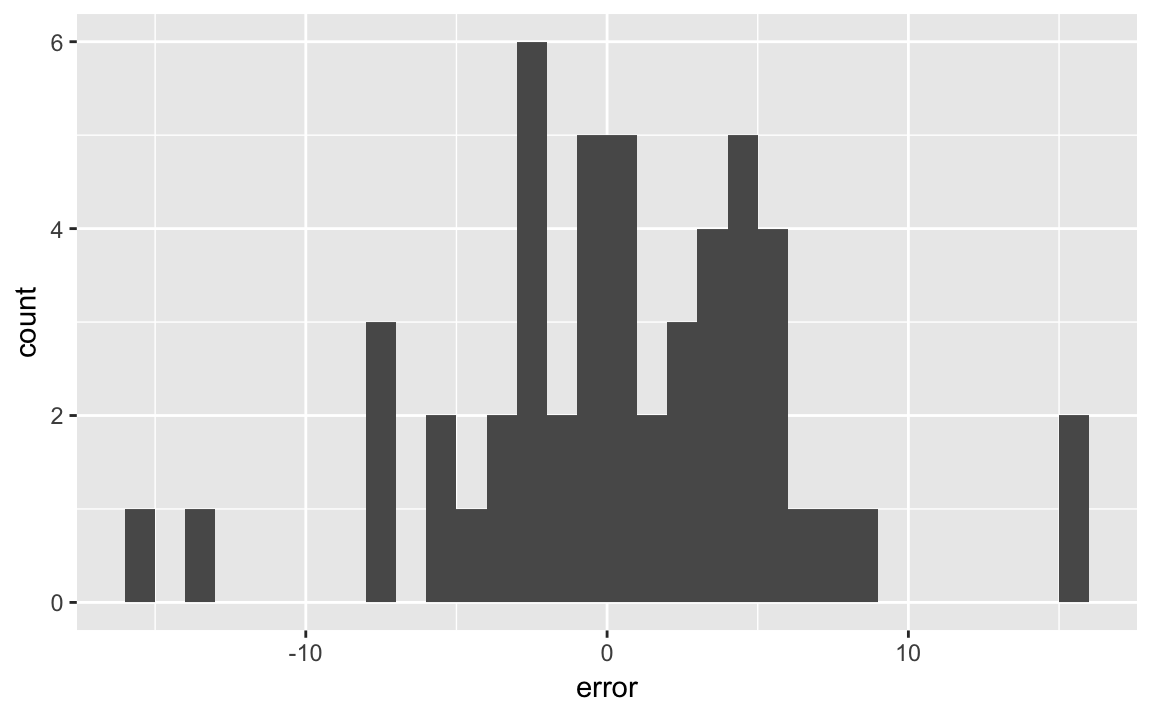
\includegraphics[width=0.7\linewidth]{prediction_files/figure-latex/unnamed-chunk-31-1} \end{center}

The text uses bin widths of 5\%:

\begin{Shaded}
\begin{Highlighting}[]
\KeywordTok{ggplot}\NormalTok{(last_polls, }\KeywordTok{aes}\NormalTok{(}\DataTypeTok{x =}\NormalTok{ error)) }\OperatorTok{+}
\StringTok{  }\KeywordTok{geom_histogram}\NormalTok{(}\DataTypeTok{binwidth =} \DecValTok{5}\NormalTok{, }\DataTypeTok{boundary =} \DecValTok{0}\NormalTok{)}
\end{Highlighting}
\end{Shaded}

\begin{center}\includegraphics[width=0.7\linewidth]{prediction_files/figure-latex/unnamed-chunk-32-1} \end{center}

\textbf{Challenge:} What other ways could you visualize the results? How
would you show all states? What about plotting the absolute or squared
errors instead of the errors?

\textbf{Challenge:} What happens to prediction error if you average
polls? Consider averaging back over time? What happens if you take the
averages of the state poll average and average of \textbf{all} polls -
does that improve prediction?

To create a scatter plots using the state abbreviations instead of
points use
\href{http://docs.ggplot2.org/current/geom_text.html}{geom\_text}
instead of
\href{http://docs.ggplot2.org/current/geom_point.html}{geom\_point}.

\begin{Shaded}
\begin{Highlighting}[]
\KeywordTok{ggplot}\NormalTok{(last_polls, }\KeywordTok{aes}\NormalTok{(}\DataTypeTok{x =}\NormalTok{ margin, }\DataTypeTok{y =}\NormalTok{ elec_margin, }\DataTypeTok{label =}\NormalTok{ state)) }\OperatorTok{+}
\StringTok{  }\KeywordTok{geom_abline}\NormalTok{(}\DataTypeTok{color =} \StringTok{"white"}\NormalTok{, }\DataTypeTok{size =} \DecValTok{2}\NormalTok{) }\OperatorTok{+}
\StringTok{  }\KeywordTok{geom_hline}\NormalTok{(}\DataTypeTok{yintercept =} \DecValTok{0}\NormalTok{, }\DataTypeTok{color =} \StringTok{"gray"}\NormalTok{, }\DataTypeTok{size =} \DecValTok{2}\NormalTok{) }\OperatorTok{+}
\StringTok{  }\KeywordTok{geom_vline}\NormalTok{(}\DataTypeTok{xintercept =} \DecValTok{0}\NormalTok{, }\DataTypeTok{color =} \StringTok{"gray"}\NormalTok{, }\DataTypeTok{size =} \DecValTok{2}\NormalTok{) }\OperatorTok{+}
\StringTok{  }\KeywordTok{geom_text}\NormalTok{() }\OperatorTok{+}
\StringTok{  }\KeywordTok{coord_fixed}\NormalTok{() }\OperatorTok{+}
\StringTok{  }\KeywordTok{labs}\NormalTok{(}\DataTypeTok{x =} \StringTok{"Poll Results"}\NormalTok{, }\DataTypeTok{y =} \StringTok{"Actual Election Results"}\NormalTok{)}
\end{Highlighting}
\end{Shaded}

\begin{center}\includegraphics[width=0.7\linewidth]{prediction_files/figure-latex/unnamed-chunk-33-1} \end{center}

We can create a confusion matrix as follows. Create a new column
\texttt{classification} which shows how the poll's classification was
related to the actual election outcome (``true positive'', ``false
positive'', ``true negative'', ``false negative''). If there were two
outcomes, then we would use the function. But with more than two
outcomes, it is easier to use the
\href{https://cran.r-project.org/package=dplyr}{dplyr} function .

\begin{Shaded}
\begin{Highlighting}[]
\NormalTok{last_polls <-}
\StringTok{  }\NormalTok{last_polls }\OperatorTok
\StringTok{  }\KeywordTok{ungroup}\NormalTok{() }\OperatorTok
\StringTok{  }\KeywordTok{mutate}\NormalTok{(}\DataTypeTok{classification =}
           \KeywordTok{case_when}\NormalTok{(}
\NormalTok{             (.}\OperatorTok{$}\NormalTok{margin }\OperatorTok{>}\StringTok{ }\DecValTok{0} \OperatorTok{&}\StringTok{ }\NormalTok{.}\OperatorTok{$}\NormalTok{elec_margin }\OperatorTok{>}\StringTok{ }\DecValTok{0}\NormalTok{) }\OperatorTok{~}\StringTok{ "true positive"}\NormalTok{,}
\NormalTok{             (.}\OperatorTok{$}\NormalTok{margin }\OperatorTok{>}\StringTok{ }\DecValTok{0} \OperatorTok{&}\StringTok{ }\NormalTok{.}\OperatorTok{$}\NormalTok{elec_margin }\OperatorTok{<}\StringTok{ }\DecValTok{0}\NormalTok{) }\OperatorTok{~}\StringTok{ "false positive"}\NormalTok{,}
\NormalTok{             (.}\OperatorTok{$}\NormalTok{margin }\OperatorTok{<}\StringTok{ }\DecValTok{0} \OperatorTok{&}\StringTok{ }\NormalTok{.}\OperatorTok{$}\NormalTok{elec_margin }\OperatorTok{<}\StringTok{ }\DecValTok{0}\NormalTok{) }\OperatorTok{~}\StringTok{ "true negative"}\NormalTok{,}
\NormalTok{             (.}\OperatorTok{$}\NormalTok{margin }\OperatorTok{<}\StringTok{ }\DecValTok{0} \OperatorTok{&}\StringTok{ }\NormalTok{.}\OperatorTok{$}\NormalTok{elec_margin }\OperatorTok{>}\StringTok{ }\DecValTok{0}\NormalTok{) }\OperatorTok{~}\StringTok{ "false negative"}
\NormalTok{           ))}
\end{Highlighting}
\end{Shaded}

You need to use \texttt{.} to refer to the data frame when using
\texttt{case\_when()} within \texttt{mutate()}. Also, we needed to first
use in order to remove the grouping variable so \texttt{mutate()} will
work.

Now simply count the number of polls in each category of
\texttt{classification}:

\begin{Shaded}
\begin{Highlighting}[]
\NormalTok{last_polls }\OperatorTok
\StringTok{  }\KeywordTok{group_by}\NormalTok{(classification) }\OperatorTok
\StringTok{  }\KeywordTok{count}\NormalTok{()}
\CommentTok{#> # A tibble: 4 x 2}
\CommentTok{#> # Groups:   classification [4]}
\CommentTok{#>   classification     n}
\CommentTok{#>   <chr>          <int>}
\CommentTok{#> 1 false negative     2}
\CommentTok{#> 2 false positive     1}
\CommentTok{#> 3 true negative     21}
\CommentTok{#> 4 true positive     27}
\end{Highlighting}
\end{Shaded}

Which states were incorrectly predicted by the polls, and what was their
margins?

\begin{Shaded}
\begin{Highlighting}[]
\NormalTok{last_polls }\OperatorTok
\StringTok{  }\KeywordTok{filter}\NormalTok{(classification }\OperatorTok\StringTok{ }\KeywordTok{c}\NormalTok{(}\StringTok{"false positive"}\NormalTok{, }\StringTok{"false negative"}\NormalTok{)) }\OperatorTok
\StringTok{  }\KeywordTok{select}\NormalTok{(state, margin, elec_margin, classification) }\OperatorTok
\StringTok{  }\KeywordTok{arrange}\NormalTok{(}\KeywordTok{desc}\NormalTok{(elec_margin))}
\CommentTok{#> # A tibble: 3 x 4}
\CommentTok{#>   state margin elec_margin classification}
\CommentTok{#>   <chr>  <int>       <int> <chr>         }
\CommentTok{#> 1 IN        -5           1 false negative}
\CommentTok{#> 2 NC        -1           1 false negative}
\CommentTok{#> 3 MO         1          -1 false positive}
\end{Highlighting}
\end{Shaded}

What was the difference in the poll prediction of electoral votes and
actual electoral votes? We hadn't included the variable \texttt{EV} when
we first merged, but that's no problem, we'll just merge again in order
to grab that variable:

\begin{Shaded}
\begin{Highlighting}[]
\NormalTok{last_polls }\OperatorTok
\StringTok{  }\KeywordTok{left_join}\NormalTok{(}\KeywordTok{select}\NormalTok{(pres08, state, EV), }\DataTypeTok{by =} \StringTok{"state"}\NormalTok{) }\OperatorTok
\StringTok{  }\KeywordTok{summarise}\NormalTok{(}\DataTypeTok{EV_pred =} \KeywordTok{sum}\NormalTok{( (margin }\OperatorTok{>}\StringTok{ }\DecValTok{0}\NormalTok{) }\OperatorTok{*}\StringTok{ }\NormalTok{EV),}
            \DataTypeTok{EV_actual =} \KeywordTok{sum}\NormalTok{( (elec_margin }\OperatorTok{>}\StringTok{ }\DecValTok{0}\NormalTok{) }\OperatorTok{*}\StringTok{ }\NormalTok{EV))}
\CommentTok{#> # A tibble: 1 x 2}
\CommentTok{#>   EV_pred EV_actual}
\CommentTok{#>     <int>     <int>}
\CommentTok{#> 1     349       364}
\end{Highlighting}
\end{Shaded}

\begin{Shaded}
\begin{Highlighting}[]
\KeywordTok{data}\NormalTok{(}\StringTok{"pollsUS08"}\NormalTok{, }\DataTypeTok{package =} \StringTok{"qss"}\NormalTok{)}
\end{Highlighting}
\end{Shaded}

\begin{Shaded}
\begin{Highlighting}[]
\NormalTok{pollsUS08 <-}\StringTok{ }\KeywordTok{mutate}\NormalTok{(pollsUS08, }\DataTypeTok{DaysToElection =}\NormalTok{ ELECTION_DAY }\OperatorTok{-}\StringTok{ }\NormalTok{middate)}
\end{Highlighting}
\end{Shaded}

We'll produce the seven-day averages slightly differently than the
method used in the text. For all dates in the data, we'll calculate the
moving average. The code presented in \emph{QSS} uses a for loop similar
to the following:

\begin{Shaded}
\begin{Highlighting}[]
\NormalTok{all_dates <-}\StringTok{ }\KeywordTok{seq}\NormalTok{(}\KeywordTok{min}\NormalTok{(polls08}\OperatorTok{$}\NormalTok{middate), ELECTION_DAY, }\DataTypeTok{by =} \StringTok{"days"}\NormalTok{)}

\CommentTok{# Number of poll days to use}
\NormalTok{POLL_DAYS <-}\StringTok{ }\DecValTok{7}

\NormalTok{pop_vote_avg <-}\StringTok{ }\KeywordTok{vector}\NormalTok{(}\KeywordTok{length}\NormalTok{(all_dates), }\DataTypeTok{mode =} \StringTok{"list"}\NormalTok{)}
\ControlFlowTok{for}\NormalTok{ (i }\ControlFlowTok{in} \KeywordTok{seq_along}\NormalTok{(all_dates)) \{}
\NormalTok{  date <-}\StringTok{ }\NormalTok{all_dates[i]}
  \CommentTok{# summarise the seven day}
\NormalTok{  week_data <-}
\StringTok{     }\KeywordTok{filter}\NormalTok{(polls08,}
            \KeywordTok{as.integer}\NormalTok{(middate }\OperatorTok{-}\StringTok{ }\NormalTok{date) }\OperatorTok{<=}\StringTok{ }\DecValTok{0}\NormalTok{,}
            \KeywordTok{as.integer}\NormalTok{(middate }\OperatorTok{-}\StringTok{ }\NormalTok{date) }\OperatorTok{>}\StringTok{ }\OperatorTok{-}\StringTok{ }\NormalTok{POLL_DAYS) }\OperatorTok
\StringTok{     }\KeywordTok{summarise}\NormalTok{(}\DataTypeTok{Obama =} \KeywordTok{mean}\NormalTok{(Obama, }\DataTypeTok{na.rm =} \OtherTok{TRUE}\NormalTok{),}
               \DataTypeTok{McCain =} \KeywordTok{mean}\NormalTok{(McCain, }\DataTypeTok{na.rm =} \OtherTok{TRUE}\NormalTok{))}
  \CommentTok{# add date for the observation}
\NormalTok{  week_data}\OperatorTok{$}\NormalTok{date <-}\StringTok{ }\NormalTok{date}
\NormalTok{  pop_vote_avg[[i]] <-}\StringTok{ }\NormalTok{week_data}
\NormalTok{\}}

\NormalTok{pop_vote_avg <-}\StringTok{ }\KeywordTok{bind_rows}\NormalTok{(pop_vote_avg)}
\end{Highlighting}
\end{Shaded}

Write a function which takes a \texttt{date}, and calculates the
\texttt{days} (set the default to 7 days) moving average using the
dataset \texttt{.data}:

\begin{Shaded}
\begin{Highlighting}[]
\NormalTok{poll_ma <-}\StringTok{ }\ControlFlowTok{function}\NormalTok{(date, .data, }\DataTypeTok{days =} \DecValTok{7}\NormalTok{) \{}
  \KeywordTok{filter}\NormalTok{(.data,}
        \KeywordTok{as.integer}\NormalTok{(middate }\OperatorTok{-}\StringTok{ }\NormalTok{date) }\OperatorTok{<=}\StringTok{ }\DecValTok{0}\NormalTok{,}
        \KeywordTok{as.integer}\NormalTok{(middate }\OperatorTok{-}\StringTok{ }\NormalTok{date) }\OperatorTok{>}\StringTok{ }\OperatorTok{-}\StringTok{ }\OperatorTok{!!}\NormalTok{days) }\OperatorTok
\StringTok{  }\KeywordTok{summarise}\NormalTok{(}\DataTypeTok{Obama =} \KeywordTok{mean}\NormalTok{(Obama, }\DataTypeTok{na.rm =} \OtherTok{TRUE}\NormalTok{),}
           \DataTypeTok{McCain =} \KeywordTok{mean}\NormalTok{(McCain, }\DataTypeTok{na.rm =} \OtherTok{TRUE}\NormalTok{)) }\OperatorTok
\StringTok{  }\KeywordTok{mutate}\NormalTok{(}\DataTypeTok{date =} \OperatorTok{!!}\NormalTok{date)}
\NormalTok{\}}
\end{Highlighting}
\end{Shaded}

The code above uses \texttt{!!}. This tells \texttt{filter} that
\texttt{days} refers to a variable \texttt{days} in the calling
environment, and not a column named \texttt{days} in the data frame. In
this case, there wouldn't be any ambiguities since there is not a column
named \texttt{days}, but in general there can be ambiguities in the
dplyr functions as to whether the names refer to columns in the data
frame or variables in the environment calling the function. Read
\href{http://dplyr.tidyverse.org/articles/programming.html}{Programming
with dplyr} for an in-depth discussion of this.

This returns a one row data frame with the moving average for McCain and
Obama on Nov 1, 2008.

\begin{Shaded}
\begin{Highlighting}[]
\KeywordTok{poll_ma}\NormalTok{(}\KeywordTok{as.Date}\NormalTok{(}\StringTok{"2008-11-01"}\NormalTok{), polls08)}
\CommentTok{#>   Obama McCain       date}
\CommentTok{#> 1  49.1   45.4 2008-11-01}
\end{Highlighting}
\end{Shaded}

Since we made \texttt{days} an argument to the function we could easily
change the code to calculate other moving averages,

\begin{Shaded}
\begin{Highlighting}[]
\KeywordTok{poll_ma}\NormalTok{(}\KeywordTok{as.Date}\NormalTok{(}\StringTok{"2008-11-01"}\NormalTok{), polls08, }\DataTypeTok{days =} \DecValTok{3}\NormalTok{)}
\CommentTok{#>   Obama McCain       date}
\CommentTok{#> 1  50.6   45.4 2008-11-01}
\end{Highlighting}
\end{Shaded}

Now use a functional to execute that function with all dates for which
we want moving averages. The function \texttt{poll\_ma} returns a data
frame, and our ideal output is a data frame that stacks those data
frames row-wise. So we will use the \texttt{map\_df} function,

\begin{Shaded}
\begin{Highlighting}[]
\KeywordTok{map_df}\NormalTok{(all_dates, poll_ma, polls08)}
\end{Highlighting}
\end{Shaded}

Note that the other arguments for \texttt{poll\_ma} are placed after the
name of the function as additional arguments to \texttt{map\_df}.

It is easier to plot this if the data are tidy, with \texttt{Obama} and
\texttt{McCain} as categories of a column \texttt{candidate}.

\begin{Shaded}
\begin{Highlighting}[]
\NormalTok{pop_vote_avg_tidy <-}
\StringTok{  }\NormalTok{pop_vote_avg }\OperatorTok
\StringTok{  }\KeywordTok{gather}\NormalTok{(candidate, share, }\OperatorTok{-}\NormalTok{date, }\DataTypeTok{na.rm =} \OtherTok{TRUE}\NormalTok{)}
\KeywordTok{head}\NormalTok{(pop_vote_avg_tidy)}
\CommentTok{#>         date candidate share}
\CommentTok{#> 1 2008-01-01     Obama  46.5}
\CommentTok{#> 2 2008-01-02     Obama  46.5}
\CommentTok{#> 3 2008-01-03     Obama  46.5}
\CommentTok{#> 4 2008-01-04     Obama  46.5}
\CommentTok{#> 5 2008-01-05     Obama  46.5}
\CommentTok{#> 6 2008-01-06     Obama  46.5}
\end{Highlighting}
\end{Shaded}

\begin{Shaded}
\begin{Highlighting}[]
\KeywordTok{ggplot}\NormalTok{(pop_vote_avg_tidy, }\KeywordTok{aes}\NormalTok{(}\DataTypeTok{x =}\NormalTok{ date, }\DataTypeTok{y =}\NormalTok{ share,}
                              \DataTypeTok{colour =} \KeywordTok{fct_reorder2}\NormalTok{(candidate, date, share))) }\OperatorTok{+}
\StringTok{  }\KeywordTok{geom_point}\NormalTok{() }\OperatorTok{+}
\StringTok{  }\KeywordTok{geom_line}\NormalTok{() }\OperatorTok{+}
\StringTok{  }\KeywordTok{scale_colour_manual}\NormalTok{(}\StringTok{"Candidate"}\NormalTok{,}
                      \DataTypeTok{values =} \KeywordTok{c}\NormalTok{(}\DataTypeTok{Obama =} \StringTok{"blue"}\NormalTok{, }\DataTypeTok{McCain =} \StringTok{"red"}\NormalTok{))}
\end{Highlighting}
\end{Shaded}

\begin{center}\includegraphics[width=0.7\linewidth]{prediction_files/figure-latex/unnamed-chunk-46-1} \end{center}

\textbf{Challenge} read \href{http://r4ds.had.co.nz/}{R for Data
Science} chapter
\href{http://r4ds.had.co.nz/iteration.html\#the-map-functions}{Iteration}
and use the function
\href{https://www.rdocumentation.org/packages/purrr/topics/map_df}{map\_df}
to create the object \texttt{poll\_vote\_avg} as above instead of a for
loop.

The 7-day average is similar to the simple method used by
\href{http://www.realclearpolitics.com/epolls/2016/president/us/general_election_trump_vs_clinton-5491.html}{Real
Clear Politics}. The RCP average is simply the average of all polls in
their data for the last seven days. Sites like
\href{https://fivethirtyeight.com}{538} and the
\href{http://elections.huffingtonpost.com/pollster}{Huffpost Pollster},
on the other hand, also use what amounts to averaging polls, but using
more sophisticated statistical methods to assign different weights to
different polls.

\textbf{Challenge} Why do we need to use different polls for the popular
vote data? Why not simply average all the state polls? What would you
have to do? Would the overall popular vote be useful in predicting
state-level polling, or vice-versa? How would you use them?

\hypertarget{linear-regression}{%
\section{Linear Regression}\label{linear-regression}}

\hypertarget{facial-appearance-and-election-outcomes}{%
\subsection{Facial Appearance and Election
Outcomes}\label{facial-appearance-and-election-outcomes}}

Load the \texttt{face} dataset:

\begin{Shaded}
\begin{Highlighting}[]
\KeywordTok{data}\NormalTok{(}\StringTok{"face"}\NormalTok{, }\DataTypeTok{package =} \StringTok{"qss"}\NormalTok{)}
\end{Highlighting}
\end{Shaded}

Add Democrat and Republican vote shares, and the difference in shares:

\begin{Shaded}
\begin{Highlighting}[]
\NormalTok{face <-}\StringTok{ }\KeywordTok{mutate}\NormalTok{(face,}
                \DataTypeTok{d.share =}\NormalTok{ d.votes }\OperatorTok{/}\StringTok{ }\NormalTok{(d.votes }\OperatorTok{+}\StringTok{ }\NormalTok{r.votes),}
                \DataTypeTok{r.share =}\NormalTok{ r.votes }\OperatorTok{/}\StringTok{ }\NormalTok{(d.votes }\OperatorTok{+}\StringTok{ }\NormalTok{r.votes),}
                \DataTypeTok{diff.share =}\NormalTok{ d.share }\OperatorTok{-}\StringTok{ }\NormalTok{r.share)}
\end{Highlighting}
\end{Shaded}

Plot facial competence vs.~vote share:

\begin{Shaded}
\begin{Highlighting}[]
\KeywordTok{ggplot}\NormalTok{(face, }\KeywordTok{aes}\NormalTok{(}\DataTypeTok{x =}\NormalTok{ d.comp, }\DataTypeTok{y =}\NormalTok{ diff.share, }\DataTypeTok{colour =}\NormalTok{ w.party)) }\OperatorTok{+}
\StringTok{  }\KeywordTok{geom_ref_line}\NormalTok{(}\DataTypeTok{h =} \DecValTok{0}\NormalTok{) }\OperatorTok{+}
\StringTok{  }\KeywordTok{geom_point}\NormalTok{() }\OperatorTok{+}
\StringTok{  }\KeywordTok{scale_colour_manual}\NormalTok{(}\StringTok{"Winning}\CharTok{\textbackslash{}n}\StringTok{Party"}\NormalTok{,}
                      \DataTypeTok{values =} \KeywordTok{c}\NormalTok{(}\DataTypeTok{D =} \StringTok{"blue"}\NormalTok{, }\DataTypeTok{R =} \StringTok{"red"}\NormalTok{)) }\OperatorTok{+}
\StringTok{  }\KeywordTok{labs}\NormalTok{(}\DataTypeTok{x =} \StringTok{"Competence scores for Democrats"}\NormalTok{,}
       \DataTypeTok{y =} \StringTok{"Democratic margin in vote share"}\NormalTok{)}
\end{Highlighting}
\end{Shaded}

\begin{center}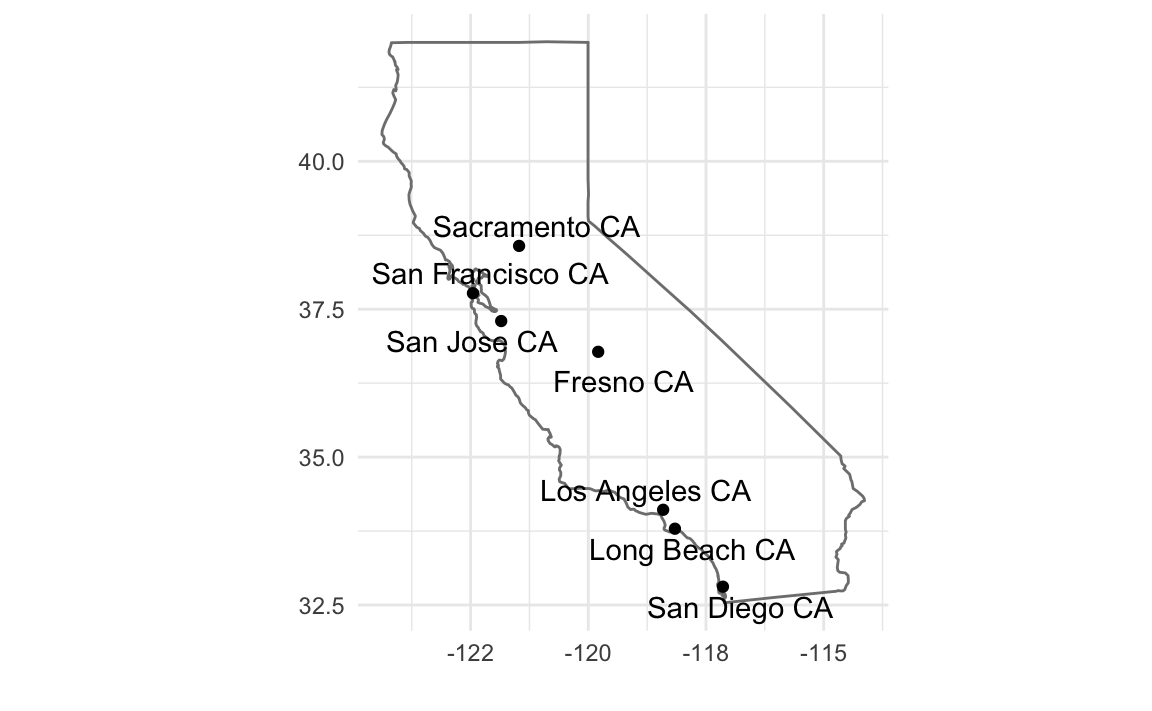
\includegraphics[width=0.7\linewidth]{prediction_files/figure-latex/unnamed-chunk-47-1} \end{center}

\hypertarget{correlation-and-scatter-plots}{%
\subsection{Correlation and Scatter
Plots}\label{correlation-and-scatter-plots}}

\begin{Shaded}
\begin{Highlighting}[]
\KeywordTok{cor}\NormalTok{(face}\OperatorTok{$}\NormalTok{d.comp, face}\OperatorTok{$}\NormalTok{diff.share)}
\CommentTok{#> [1] 0.433}
\end{Highlighting}
\end{Shaded}

\hypertarget{least-squares}{%
\subsection{Least Squares}\label{least-squares}}

Run the linear regression

\begin{Shaded}
\begin{Highlighting}[]
\NormalTok{fit <-}\StringTok{ }\KeywordTok{lm}\NormalTok{(diff.share }\OperatorTok{~}\StringTok{ }\NormalTok{d.comp, }\DataTypeTok{data =}\NormalTok{ face)}
\NormalTok{fit}
\CommentTok{#> }
\CommentTok{#> Call:}
\CommentTok{#> lm(formula = diff.share ~ d.comp, data = face)}
\CommentTok{#> }
\CommentTok{#> Coefficients:}
\CommentTok{#> (Intercept)       d.comp  }
\CommentTok{#>      -0.312        0.660}
\end{Highlighting}
\end{Shaded}

There are many functions to get data out of the \texttt{lm} model.

In addition to these, the
\href{https://cran.r-project.org/package=broom}{broom} package provides
three functions: \texttt{glance}, \texttt{tidy}, and \texttt{augment}
that always return data frames.

The function
\href{https://www.rdocumentation.org/packages/broom/topics/glance.lm}{glance}
returns a one-row data-frame summary of the model,

\begin{Shaded}
\begin{Highlighting}[]
\KeywordTok{glance}\NormalTok{(fit)}
\CommentTok{#>   r.squared adj.r.squared sigma statistic  p.value df logLik AIC  BIC}
\CommentTok{#> 1     0.187          0.18 0.266        27 8.85e-07  2  -10.5  27 35.3}
\CommentTok{#>   deviance df.residual}
\CommentTok{#> 1     8.31         117}
\end{Highlighting}
\end{Shaded}

The function
\href{https://www.rdocumentation.org/packages/broom/topics/tidy.lm}{tidy}
returns a data frame in which each row is a coefficient,

\begin{Shaded}
\begin{Highlighting}[]
\KeywordTok{tidy}\NormalTok{(fit)}
\CommentTok{#>          term estimate std.error statistic  p.value}
\CommentTok{#> 1 (Intercept)   -0.312     0.066     -4.73 6.24e-06}
\CommentTok{#> 2      d.comp    0.660     0.127      5.19 8.85e-07}
\end{Highlighting}
\end{Shaded}

The function
\href{https://www.rdocumentation.org/packages/broom/topics/augment.lm}{augment}
returns the original data with fitted values, residuals, and other
observation level stats from the model appended to it.

\begin{Shaded}
\begin{Highlighting}[]
\KeywordTok{augment}\NormalTok{(fit) }\OperatorTok\StringTok{ }\KeywordTok{head}\NormalTok{()}
\CommentTok{#>   diff.share d.comp .fitted .se.fit  .resid    .hat .sigma  .cooksd}
\CommentTok{#> 1     0.2101  0.565  0.0606  0.0266  0.1495 0.00996  0.267 0.001600}
\CommentTok{#> 2     0.1194  0.342 -0.0864  0.0302  0.2059 0.01286  0.267 0.003938}
\CommentTok{#> 3     0.0499  0.612  0.0922  0.0295 -0.0423 0.01229  0.268 0.000158}
\CommentTok{#> 4     0.1965  0.542  0.0454  0.0256  0.1511 0.00922  0.267 0.001510}
\CommentTok{#> 5     0.4958  0.680  0.1370  0.0351  0.3588 0.01737  0.266 0.016307}
\CommentTok{#> 6    -0.3495  0.321 -0.1006  0.0319 -0.2490 0.01433  0.267 0.006436}
\CommentTok{#>   .std.resid}
\CommentTok{#> 1      0.564}
\CommentTok{#> 2      0.778}
\CommentTok{#> 3     -0.160}
\CommentTok{#> 4      0.570}
\CommentTok{#> 5      1.358}
\CommentTok{#> 6     -0.941}
\end{Highlighting}
\end{Shaded}

We can plot the results of the bivariate linear regression as follows:

\begin{Shaded}
\begin{Highlighting}[]
\KeywordTok{ggplot}\NormalTok{() }\OperatorTok{+}
\StringTok{  }\KeywordTok{geom_point}\NormalTok{(}\DataTypeTok{data =}\NormalTok{ face, }\DataTypeTok{mapping =} \KeywordTok{aes}\NormalTok{(}\DataTypeTok{x =}\NormalTok{ d.comp, }\DataTypeTok{y =}\NormalTok{ diff.share)) }\OperatorTok{+}
\StringTok{  }\KeywordTok{geom_ref_line}\NormalTok{(}\DataTypeTok{v =} \KeywordTok{mean}\NormalTok{(face}\OperatorTok{$}\NormalTok{d.comp)) }\OperatorTok{+}
\StringTok{  }\KeywordTok{geom_ref_line}\NormalTok{(}\DataTypeTok{h =} \KeywordTok{mean}\NormalTok{(face}\OperatorTok{$}\NormalTok{diff.share)) }\OperatorTok{+}
\StringTok{  }\KeywordTok{geom_abline}\NormalTok{(}\DataTypeTok{slope =} \KeywordTok{coef}\NormalTok{(fit)[}\StringTok{"d.comp"}\NormalTok{],}
              \DataTypeTok{intercept =} \KeywordTok{coef}\NormalTok{(fit)[}\StringTok{"(Intercept)"}\NormalTok{],}
              \DataTypeTok{colour =} \StringTok{"red"}\NormalTok{) }\OperatorTok{+}
\StringTok{  }\KeywordTok{annotate}\NormalTok{(}\StringTok{"text"}\NormalTok{, }\DataTypeTok{x =} \FloatTok{0.9}\NormalTok{, }\DataTypeTok{y =} \KeywordTok{mean}\NormalTok{(face}\OperatorTok{$}\NormalTok{diff.share) }\OperatorTok{+}\StringTok{ }\FloatTok{0.05}\NormalTok{,}
           \DataTypeTok{label =} \StringTok{"Mean of Y"}\NormalTok{, }\DataTypeTok{color =} \StringTok{"blue"}\NormalTok{, }\DataTypeTok{vjust =} \DecValTok{0}\NormalTok{) }\OperatorTok{+}
\StringTok{  }\KeywordTok{annotate}\NormalTok{(}\StringTok{"text"}\NormalTok{, }\DataTypeTok{y =} \FloatTok{-0.9}\NormalTok{, }\DataTypeTok{x =} \KeywordTok{mean}\NormalTok{(face}\OperatorTok{$}\NormalTok{d.comp), }\DataTypeTok{label =} \StringTok{"Mean of X"}\NormalTok{,}
           \DataTypeTok{color =} \StringTok{"blue"}\NormalTok{, }\DataTypeTok{hjust =} \DecValTok{0}\NormalTok{) }\OperatorTok{+}
\StringTok{  }\KeywordTok{scale_y_continuous}\NormalTok{(}\StringTok{"Democratic margin in vote shares"}\NormalTok{,}
                     \DataTypeTok{breaks =} \KeywordTok{seq}\NormalTok{(}\OperatorTok{-}\DecValTok{1}\NormalTok{, }\DecValTok{1}\NormalTok{, }\DataTypeTok{by =} \FloatTok{0.5}\NormalTok{), }\DataTypeTok{limits =} \KeywordTok{c}\NormalTok{(}\OperatorTok{-}\DecValTok{1}\NormalTok{, }\DecValTok{1}\NormalTok{)) }\OperatorTok{+}
\StringTok{  }\KeywordTok{scale_x_continuous}\NormalTok{(}\StringTok{"Democratic margin in vote shares"}\NormalTok{,}
                     \DataTypeTok{breaks =} \KeywordTok{seq}\NormalTok{(}\DecValTok{0}\NormalTok{, }\DecValTok{1}\NormalTok{, }\DataTypeTok{by =} \FloatTok{0.2}\NormalTok{), }\DataTypeTok{limits =} \KeywordTok{c}\NormalTok{(}\DecValTok{0}\NormalTok{, }\DecValTok{1}\NormalTok{)) }\OperatorTok{+}
\StringTok{  }\KeywordTok{ggtitle}\NormalTok{(}\StringTok{"Facial compotence and vote share"}\NormalTok{)}
\end{Highlighting}
\end{Shaded}

\begin{center}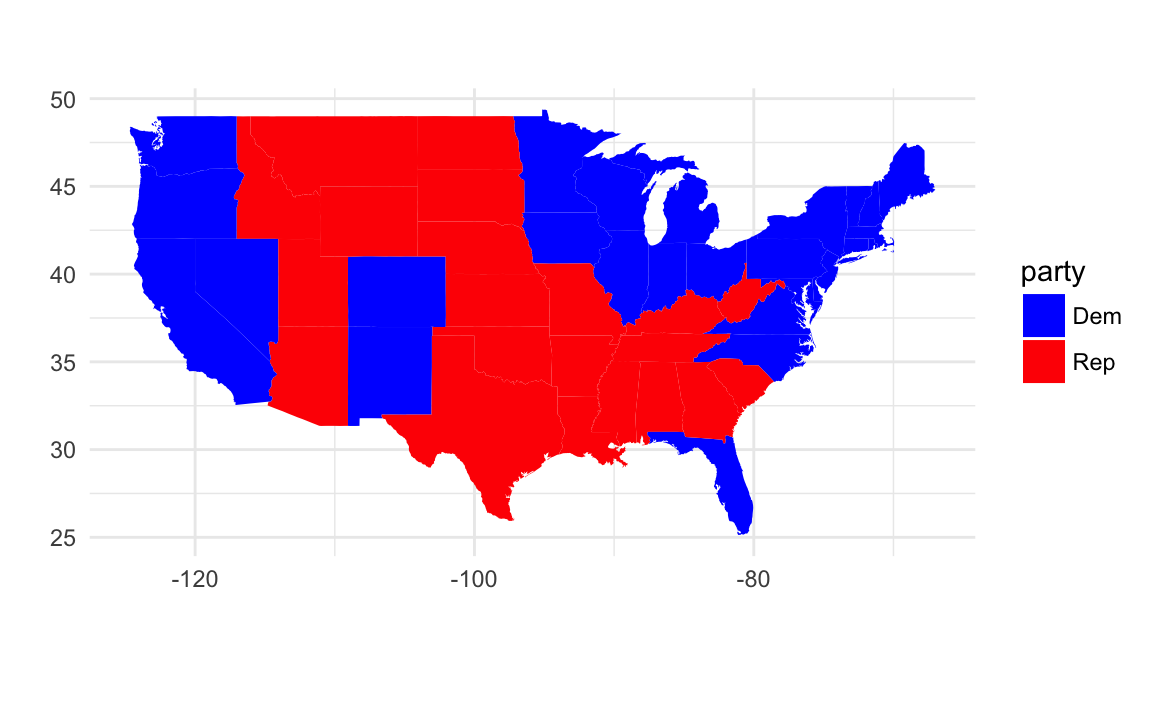
\includegraphics[width=0.7\linewidth]{prediction_files/figure-latex/unnamed-chunk-53-1} \end{center}

A more general way to plot the predictions of the model against the data
is to use the methods described in
\href{http://r4ds.had.co.nz/model-basics.html\#visualising-models}{Ch
23.3.3} of R4DS. Create an evenly spaced grid of values of
\texttt{d.comp}, and add predictions of the model to it.

\begin{Shaded}
\begin{Highlighting}[]
\NormalTok{grid <-}\StringTok{ }\NormalTok{face }\OperatorTok
\StringTok{  }\KeywordTok{data_grid}\NormalTok{(d.comp) }\OperatorTok
\StringTok{  }\KeywordTok{add_predictions}\NormalTok{(fit)}
\KeywordTok{head}\NormalTok{(grid)}
\CommentTok{#> # A tibble: 6 x 2}
\CommentTok{#>   d.comp   pred}
\CommentTok{#>    <dbl>  <dbl>}
\CommentTok{#> 1 0.0640 -0.270}
\CommentTok{#> 2 0.0847 -0.256}
\CommentTok{#> 3 0.0893 -0.253}
\CommentTok{#> 4 0.115  -0.237}
\CommentTok{#> 5 0.115  -0.236}
\CommentTok{#> 6 0.164  -0.204}
\end{Highlighting}
\end{Shaded}

Now we can plot the regression line and the original data just like any
other plot.

\begin{Shaded}
\begin{Highlighting}[]
\KeywordTok{ggplot}\NormalTok{() }\OperatorTok{+}
\StringTok{  }\KeywordTok{geom_point}\NormalTok{(}\DataTypeTok{data =}\NormalTok{ face, }\DataTypeTok{mapping =} \KeywordTok{aes}\NormalTok{(}\DataTypeTok{x =}\NormalTok{ d.comp, }\DataTypeTok{y =}\NormalTok{ diff.share)) }\OperatorTok{+}
\StringTok{  }\KeywordTok{geom_line}\NormalTok{(}\DataTypeTok{data =}\NormalTok{ grid, }\DataTypeTok{mapping =} \KeywordTok{aes}\NormalTok{(}\DataTypeTok{x =}\NormalTok{ d.comp, }\DataTypeTok{y =}\NormalTok{ pred),}
            \DataTypeTok{colour =} \StringTok{"red"}\NormalTok{)}
\end{Highlighting}
\end{Shaded}

\begin{center}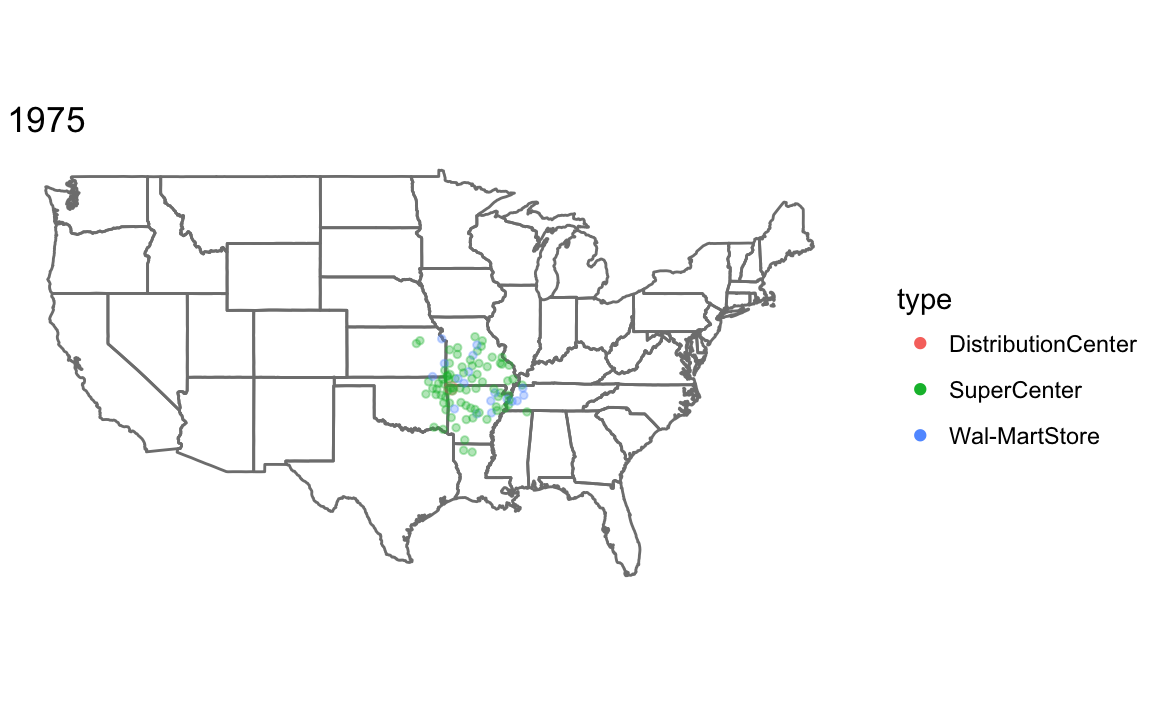
\includegraphics[width=0.7\linewidth]{prediction_files/figure-latex/unnamed-chunk-55-1} \end{center}

This method is more complicated than the \texttt{geom\_abline} method
for a bivariate regression, but will work for more complicated models,
while the \texttt{geom\_abline} method won't.

Note that
\href{http://docs.ggplot2.org/current/geom_smooth.html}{geom\_smooth}
can be used to add a regression line to a data-set.

\begin{Shaded}
\begin{Highlighting}[]
\KeywordTok{ggplot}\NormalTok{(}\DataTypeTok{data =}\NormalTok{ face, }\DataTypeTok{mapping =} \KeywordTok{aes}\NormalTok{(}\DataTypeTok{x =}\NormalTok{ d.comp, }\DataTypeTok{y =}\NormalTok{ diff.share)) }\OperatorTok{+}
\StringTok{  }\KeywordTok{geom_point}\NormalTok{() }\OperatorTok{+}
\StringTok{  }\KeywordTok{geom_smooth}\NormalTok{(}\DataTypeTok{method =} \StringTok{"lm"}\NormalTok{, }\DataTypeTok{se =} \OtherTok{FALSE}\NormalTok{)}
\end{Highlighting}
\end{Shaded}

\begin{center}\includegraphics[width=0.7\linewidth]{prediction_files/figure-latex/unnamed-chunk-56-1} \end{center}

The argument \texttt{method\ =\ "lm"} specifies that the function
\texttt{lm} is to be used to generate fitted values. It is equivalent to
running the regression \texttt{lm(y\ \textasciitilde{}\ x)} and plotting
the regression line, where \texttt{y} and \texttt{x} are the aesthetics
specified by the mappings. The argument \texttt{se\ =\ FALSE} tells the
function not to plot the confidence interval of the regression
(discussed later).

\hypertarget{regression-towards-the-mean}{%
\subsection{Regression towards the
mean}\label{regression-towards-the-mean}}

\hypertarget{merging-data-sets-in-r}{%
\subsection{Merging Data Sets in R}\label{merging-data-sets-in-r}}

See the \href{http://r4ds.had.co.nz/}{R for Data Science} chapter
\href{http://r4ds.had.co.nz/relational-data.html}{Relational data}.

\begin{Shaded}
\begin{Highlighting}[]
\KeywordTok{data}\NormalTok{(}\StringTok{"pres12"}\NormalTok{, }\DataTypeTok{package =} \StringTok{"qss"}\NormalTok{)}
\end{Highlighting}
\end{Shaded}

To join both data frames

\begin{Shaded}
\begin{Highlighting}[]
\KeywordTok{full_join}\NormalTok{(pres08, pres12, }\DataTypeTok{by =} \StringTok{"state"}\NormalTok{)}
\end{Highlighting}
\end{Shaded}

However, since there are duplicate names, \texttt{.x} and \texttt{.y}
are appended.

\textbf{Challenge} What would happen if \texttt{by\ =\ "state"} was
dropped?

To avoid the duplicate names, or change them, you can rename before
merging,

\begin{Shaded}
\begin{Highlighting}[]
\KeywordTok{full_join}\NormalTok{(}\KeywordTok{select}\NormalTok{(pres08, state, }\DataTypeTok{Obama_08 =}\NormalTok{ Obama, }\DataTypeTok{McCain_08 =}\NormalTok{ McCain,}
                 \DataTypeTok{EV_08 =}\NormalTok{ EV),}
          \KeywordTok{select}\NormalTok{(pres12, state, }\DataTypeTok{Obama_12 =}\NormalTok{ Obama, }\DataTypeTok{Romney_12 =}\NormalTok{ Romney,}
                 \DataTypeTok{EV_12 =}\NormalTok{ EV),}
          \DataTypeTok{by =} \StringTok{"state"}\NormalTok{)}
\end{Highlighting}
\end{Shaded}

or use the \texttt{suffix} argument to \texttt{full\_join}

\begin{Shaded}
\begin{Highlighting}[]
\NormalTok{pres <-}\StringTok{ }\KeywordTok{full_join}\NormalTok{(pres08, pres12, }\DataTypeTok{by =} \StringTok{"state"}\NormalTok{, }\DataTypeTok{suffix =} \KeywordTok{c}\NormalTok{(}\StringTok{"_08"}\NormalTok{, }\StringTok{"_12"}\NormalTok{))}
\KeywordTok{head}\NormalTok{(pres)}
\CommentTok{#>   state.name state Obama_08 McCain EV_08 margin Obama_12 Romney EV_12}
\CommentTok{#> 1    Alabama    AL       39     60     9    -21       38     61     9}
\CommentTok{#> 2     Alaska    AK       38     59     3    -21       41     55     3}
\CommentTok{#> 3    Arizona    AZ       45     54    10     -9       45     54    11}
\CommentTok{#> 4   Arkansas    AR       39     59     6    -20       37     61     6}
\CommentTok{#> 5 California    CA       61     37    55     24       60     37    55}
\CommentTok{#> 6   Colorado    CO       54     45     9      9       51     46     9}
\end{Highlighting}
\end{Shaded}

\textbf{Challenge} Would you consider this data tidy? How would you make
it tidy?

The \textbf{dplyr} equivalent functions for
\href{https://www.rdocumentation.org/packages/base/topics/cbind}{cbind}
is
\href{https://www.rdocumentation.org/packages/dplyr/topics/bind_cols}{bind\_cols}.

\begin{Shaded}
\begin{Highlighting}[]
\NormalTok{pres <-}\StringTok{ }\NormalTok{pres }\OperatorTok
\StringTok{  }\KeywordTok{mutate}\NormalTok{(}\DataTypeTok{Obama2008_z =} \KeywordTok{as.numeric}\NormalTok{(}\KeywordTok{scale}\NormalTok{(Obama_}\DecValTok{08}\NormalTok{)),}
         \DataTypeTok{Obama2012_z =} \KeywordTok{as.numeric}\NormalTok{(}\KeywordTok{scale}\NormalTok{(Obama_}\DecValTok{12}\NormalTok{)))}
\end{Highlighting}
\end{Shaded}

Likewise,
\href{https://www.rdocumentation.org/packages/dplyr/topics/bind_cols}{bind\_cols}
concatenates data frames by row.

We need to use the \texttt{as.numeric} function because \texttt{scale()}
always returns a matrix. Omitting \texttt{as.numeric()} would not
produce an error in the code chunk above, since the columns of a data
frame can be matrices, but it would produce errors in some of the
following code if it were omitted.

Scatter plot of states with vote shares in 2008 and 2012

\begin{Shaded}
\begin{Highlighting}[]
\KeywordTok{ggplot}\NormalTok{(pres, }\KeywordTok{aes}\NormalTok{(}\DataTypeTok{x =}\NormalTok{ Obama2008_z, }\DataTypeTok{y =}\NormalTok{ Obama2012_z, }\DataTypeTok{label =}\NormalTok{ state)) }\OperatorTok{+}
\StringTok{  }\KeywordTok{geom_abline}\NormalTok{(}\DataTypeTok{colour =} \StringTok{"white"}\NormalTok{, }\DataTypeTok{size =} \DecValTok{2}\NormalTok{) }\OperatorTok{+}
\StringTok{  }\KeywordTok{geom_text}\NormalTok{() }\OperatorTok{+}
\StringTok{  }\KeywordTok{coord_fixed}\NormalTok{() }\OperatorTok{+}
\StringTok{  }\KeywordTok{scale_x_continuous}\NormalTok{(}\StringTok{"Obama's standardized vote share in 2008"}\NormalTok{,}
                     \DataTypeTok{limits =} \KeywordTok{c}\NormalTok{(}\OperatorTok{-}\DecValTok{4}\NormalTok{, }\DecValTok{4}\NormalTok{)) }\OperatorTok{+}
\StringTok{  }\KeywordTok{scale_y_continuous}\NormalTok{(}\StringTok{"Obama's standardized vote share in 2012"}\NormalTok{,}
                     \DataTypeTok{limits =} \KeywordTok{c}\NormalTok{(}\OperatorTok{-}\DecValTok{4}\NormalTok{, }\DecValTok{4}\NormalTok{))}
\end{Highlighting}
\end{Shaded}

\begin{center}\includegraphics[width=0.7\linewidth]{prediction_files/figure-latex/unnamed-chunk-61-1} \end{center}

To calculate the bottom and top quartiles

\begin{Shaded}
\begin{Highlighting}[]
\NormalTok{pres }\OperatorTok
\StringTok{  }\KeywordTok{filter}\NormalTok{(Obama2008_z }\OperatorTok{<}\StringTok{ }\KeywordTok{quantile}\NormalTok{(Obama2008_z, }\FloatTok{0.25}\NormalTok{)) }\OperatorTok
\StringTok{  }\KeywordTok{summarise}\NormalTok{(}\DataTypeTok{improve =} \KeywordTok{mean}\NormalTok{(Obama2012_z }\OperatorTok{>}\StringTok{ }\NormalTok{Obama2008_z))}
\CommentTok{#>   improve}
\CommentTok{#> 1   0.583}

\NormalTok{pres }\OperatorTok
\StringTok{  }\KeywordTok{filter}\NormalTok{(Obama2008_z }\OperatorTok{<}\StringTok{ }\KeywordTok{quantile}\NormalTok{(Obama2008_z, }\FloatTok{0.75}\NormalTok{)) }\OperatorTok
\StringTok{  }\KeywordTok{summarise}\NormalTok{(}\DataTypeTok{improve =} \KeywordTok{mean}\NormalTok{(Obama2012_z }\OperatorTok{>}\StringTok{ }\NormalTok{Obama2008_z))}
\CommentTok{#>   improve}
\CommentTok{#> 1     0.5}
\end{Highlighting}
\end{Shaded}

\textbf{Challenge:} Why is it important to standardize the vote shares?

\hypertarget{model-fit}{%
\subsection{Model Fit}\label{model-fit}}

\begin{Shaded}
\begin{Highlighting}[]
\KeywordTok{data}\NormalTok{(}\StringTok{"florida"}\NormalTok{, }\DataTypeTok{package =} \StringTok{"qss"}\NormalTok{)}
\NormalTok{fit2 <-}\StringTok{ }\KeywordTok{lm}\NormalTok{(Buchanan00 }\OperatorTok{~}\StringTok{ }\NormalTok{Perot96, }\DataTypeTok{data =}\NormalTok{ florida)}
\NormalTok{fit2}
\CommentTok{#> }
\CommentTok{#> Call:}
\CommentTok{#> lm(formula = Buchanan00 ~ Perot96, data = florida)}
\CommentTok{#> }
\CommentTok{#> Coefficients:}
\CommentTok{#> (Intercept)      Perot96  }
\CommentTok{#>      1.3458       0.0359}
\end{Highlighting}
\end{Shaded}

Extract \(R ^ 2\) from the results of \texttt{summary},

\begin{Shaded}
\begin{Highlighting}[]
\KeywordTok{summary}\NormalTok{(fit2)}\OperatorTok{$}\NormalTok{r.squared}
\CommentTok{#> [1] 0.513}
\end{Highlighting}
\end{Shaded}

Alternatively, can get the R squared value from the data frame
\href{https://www.rdocumentation.org/packages/broom/topics/glance.lm}{glance}
returns:

\begin{Shaded}
\begin{Highlighting}[]
\KeywordTok{glance}\NormalTok{(fit2)}
\CommentTok{#>   r.squared adj.r.squared sigma statistic  p.value df logLik AIC BIC}
\CommentTok{#> 1     0.513         0.506   316      68.5 9.47e-12  2   -480 966 972}
\CommentTok{#>   deviance df.residual}
\CommentTok{#> 1  6506118          65}
\end{Highlighting}
\end{Shaded}

We can add predictions and residuals to the original data frame using
the \href{https://cran.r-project.org/package=modelr}{modelr} functions
\href{https://www.rdocumentation.org/packages/modelr/topics/add_residuals}{add\_residuals}
and
\href{https://www.rdocumentation.org/packages/modelr/topics/add_predictions}{add\_predictions}

\begin{Shaded}
\begin{Highlighting}[]
\NormalTok{florida <-}
\StringTok{  }\NormalTok{florida }\OperatorTok
\StringTok{  }\KeywordTok{add_predictions}\NormalTok{(fit2) }\OperatorTok
\StringTok{  }\KeywordTok{add_residuals}\NormalTok{(fit2)}
\KeywordTok{glimpse}\NormalTok{(florida)}
\CommentTok{#> Observations: 67}
\CommentTok{#> Variables: 9}
\CommentTok{#> $ county     <chr> "Alachua", "Baker", "Bay", "Bradford", "Brevard", "...}
\CommentTok{#> $ Clinton96  <int> 40144, 2273, 17020, 3356, 80416, 320736, 1794, 2712...}
\CommentTok{#> $ Dole96     <int> 25303, 3684, 28290, 4038, 87980, 142834, 1717, 2783...}
\CommentTok{#> $ Perot96    <int> 8072, 667, 5922, 819, 25249, 38964, 630, 7783, 7244...}
\CommentTok{#> $ Bush00     <int> 34124, 5610, 38637, 5414, 115185, 177323, 2873, 354...}
\CommentTok{#> $ Gore00     <int> 47365, 2392, 18850, 3075, 97318, 386561, 2155, 2964...}
\CommentTok{#> $ Buchanan00 <int> 263, 73, 248, 65, 570, 788, 90, 182, 270, 186, 122,...}
\CommentTok{#> $ pred       <dbl> 291.3, 25.3, 214.0, 30.8, 908.2, 1400.7, 24.0, 280....}
\CommentTok{#> $ resid      <dbl> -2.83e+01, 4.77e+01, 3.40e+01, 3.42e+01, -3.38e+02,...}
\end{Highlighting}
\end{Shaded}

There are now two new columns in \texttt{florida}, \texttt{pred} with
the fitted values (predictions), and \texttt{resid} with the residuals.

Use \texttt{fit2\_augment} to create a residual plot:

\begin{Shaded}
\begin{Highlighting}[]
\NormalTok{fit2_resid_plot <-}
\StringTok{  }\KeywordTok{ggplot}\NormalTok{(florida, }\KeywordTok{aes}\NormalTok{(}\DataTypeTok{x =}\NormalTok{ pred, }\DataTypeTok{y =}\NormalTok{ resid)) }\OperatorTok{+}
\StringTok{  }\KeywordTok{geom_ref_line}\NormalTok{(}\DataTypeTok{h =} \DecValTok{0}\NormalTok{) }\OperatorTok{+}
\StringTok{  }\KeywordTok{geom_point}\NormalTok{() }\OperatorTok{+}
\StringTok{  }\KeywordTok{labs}\NormalTok{(}\DataTypeTok{x =} \StringTok{"Fitted values"}\NormalTok{, }\DataTypeTok{y =} \StringTok{"residuals"}\NormalTok{)}
\NormalTok{fit2_resid_plot}
\end{Highlighting}
\end{Shaded}

\begin{center}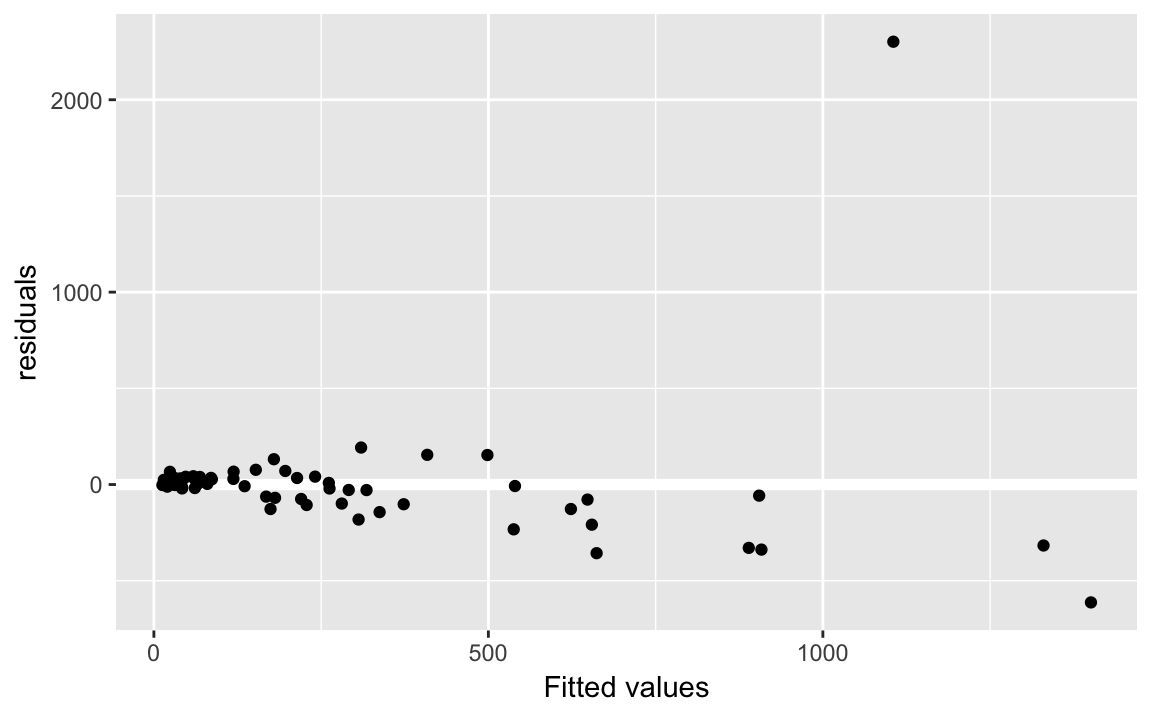
\includegraphics[width=0.7\linewidth]{prediction_files/figure-latex/unnamed-chunk-67-1} \end{center}

Note, we use the function
\href{https://www.rdocumentation.org/packages/modelr/topics/geom_refline}{geom\_refline}
to add a reference line at 0.

Let's add some labels to points, who is that outlier?

\begin{Shaded}
\begin{Highlighting}[]
\NormalTok{fit2_resid_plot }\OperatorTok{+}
\StringTok{  }\KeywordTok{geom_label}\NormalTok{(}\KeywordTok{aes}\NormalTok{(}\DataTypeTok{label =}\NormalTok{ county))}
\end{Highlighting}
\end{Shaded}

\begin{center}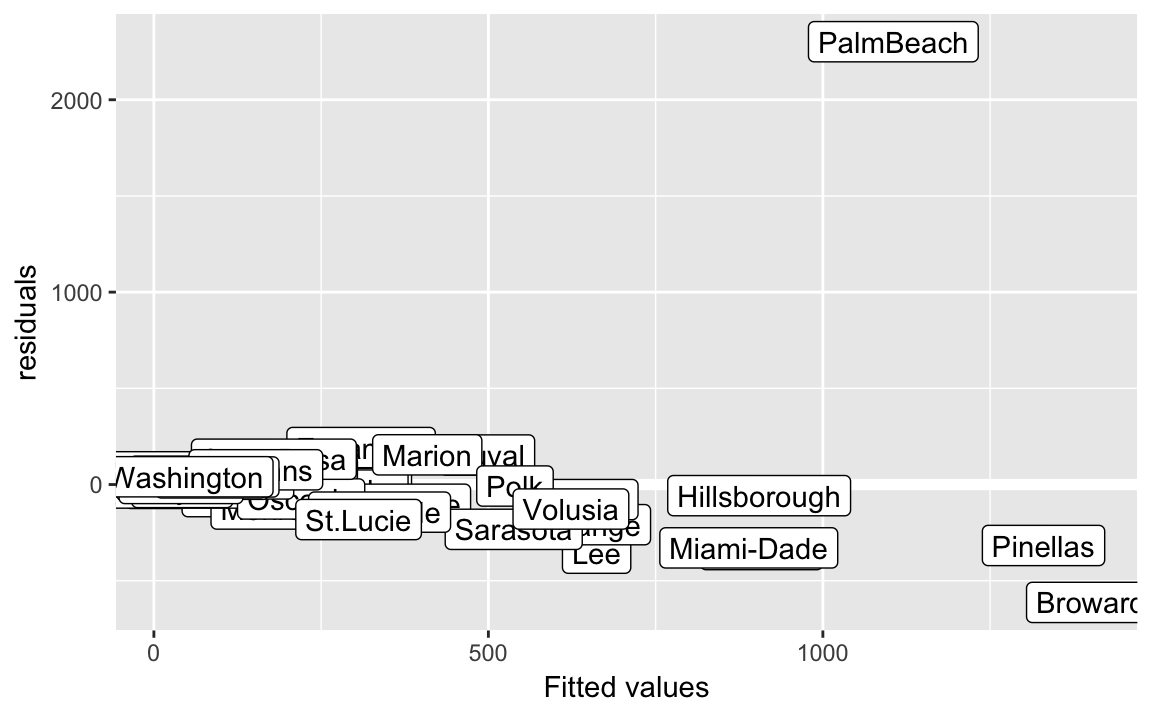
\includegraphics[width=0.7\linewidth]{prediction_files/figure-latex/unnamed-chunk-68-1} \end{center}

The outlier county is ``Palm Beach''

\begin{Shaded}
\begin{Highlighting}[]
\KeywordTok{arrange}\NormalTok{(florida) }\OperatorTok
\StringTok{  }\KeywordTok{arrange}\NormalTok{(}\KeywordTok{desc}\NormalTok{(}\KeywordTok{abs}\NormalTok{(resid))) }\OperatorTok
\StringTok{  }\KeywordTok{select}\NormalTok{(county, resid) }\OperatorTok
\StringTok{  }\KeywordTok{head}\NormalTok{()}
\CommentTok{#>       county resid}
\CommentTok{#> 1  PalmBeach  2302}
\CommentTok{#> 2    Broward  -613}
\CommentTok{#> 3        Lee  -357}
\CommentTok{#> 4    Brevard  -338}
\CommentTok{#> 5 Miami-Dade  -329}
\CommentTok{#> 6   Pinellas  -317}
\end{Highlighting}
\end{Shaded}

Data without Palm Beach

\begin{Shaded}
\begin{Highlighting}[]
\NormalTok{florida_pb <-}\StringTok{ }\KeywordTok{filter}\NormalTok{(florida, county }\OperatorTok{!=}\StringTok{ "PalmBeach"}\NormalTok{)}
\NormalTok{fit3 <-}\StringTok{ }\KeywordTok{lm}\NormalTok{(Buchanan00 }\OperatorTok{~}\StringTok{ }\NormalTok{Perot96, }\DataTypeTok{data =}\NormalTok{ florida_pb)}
\NormalTok{fit3}
\CommentTok{#> }
\CommentTok{#> Call:}
\CommentTok{#> lm(formula = Buchanan00 ~ Perot96, data = florida_pb)}
\CommentTok{#> }
\CommentTok{#> Coefficients:}
\CommentTok{#> (Intercept)      Perot96  }
\CommentTok{#>     45.8419       0.0244}
\end{Highlighting}
\end{Shaded}

\(R^2\) or coefficient of determination

\begin{Shaded}
\begin{Highlighting}[]
\KeywordTok{glance}\NormalTok{(fit3)}
\CommentTok{#>   r.squared adj.r.squared sigma statistic  p.value df logLik AIC BIC}
\CommentTok{#> 1     0.851         0.849  87.7       366 3.61e-28  2   -388 782 788}
\CommentTok{#>   deviance df.residual}
\CommentTok{#> 1   492803          64}
\end{Highlighting}
\end{Shaded}

\begin{Shaded}
\begin{Highlighting}[]
\NormalTok{florida_pb }\OperatorTok
\StringTok{  }\KeywordTok{add_residuals}\NormalTok{(fit3) }\OperatorTok
\StringTok{  }\KeywordTok{add_predictions}\NormalTok{(fit3) }\OperatorTok
\StringTok{  }\KeywordTok{ggplot}\NormalTok{(}\KeywordTok{aes}\NormalTok{(}\DataTypeTok{x =}\NormalTok{ pred, }\DataTypeTok{y =}\NormalTok{ resid)) }\OperatorTok{+}
\StringTok{  }\KeywordTok{geom_ref_line}\NormalTok{(}\DataTypeTok{h =} \DecValTok{0}\NormalTok{) }\OperatorTok{+}
\StringTok{  }\KeywordTok{geom_point}\NormalTok{() }\OperatorTok{+}
\StringTok{  }\KeywordTok{ylim}\NormalTok{(}\OperatorTok{-}\DecValTok{750}\NormalTok{, }\DecValTok{2500}\NormalTok{) }\OperatorTok{+}
\StringTok{  }\KeywordTok{xlim}\NormalTok{(}\DecValTok{0}\NormalTok{, }\DecValTok{1500}\NormalTok{) }\OperatorTok{+}
\StringTok{  }\KeywordTok{labs}\NormalTok{(}\DataTypeTok{x =} \StringTok{"Fitted values"}\NormalTok{, }\DataTypeTok{y =} \StringTok{"residuals"}\NormalTok{)}
\end{Highlighting}
\end{Shaded}

\begin{center}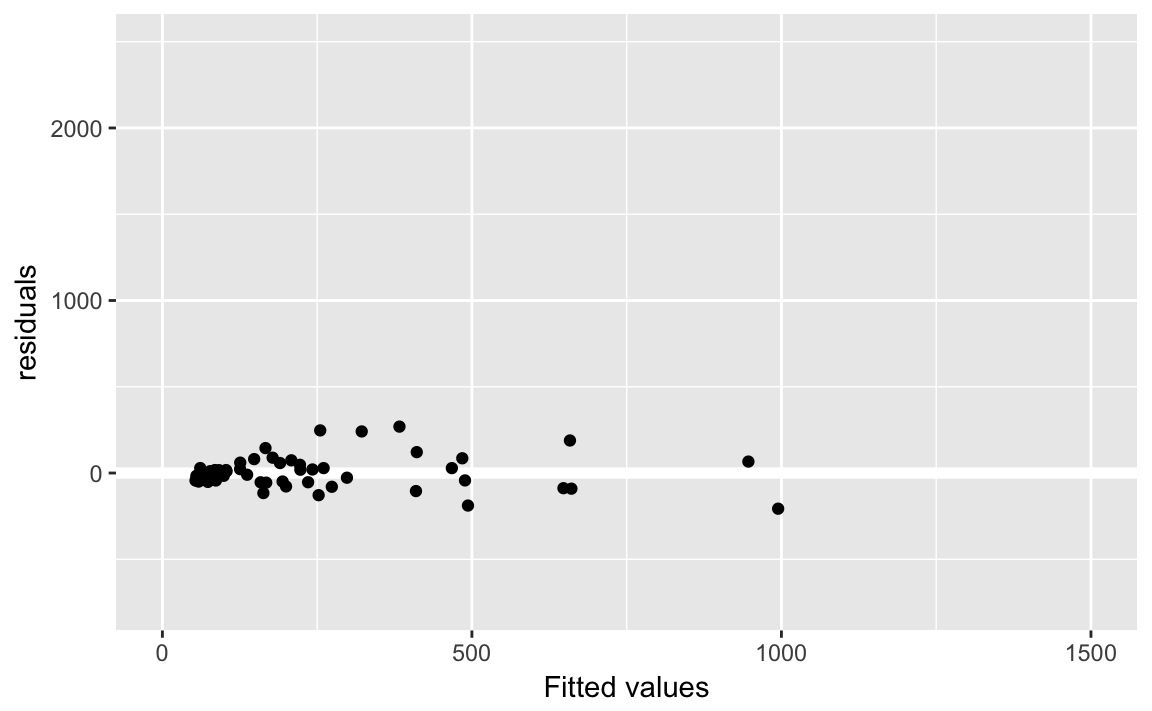
\includegraphics[width=0.7\linewidth]{prediction_files/figure-latex/unnamed-chunk-72-1} \end{center}

Create predictions for both models using
\href{https://www.rdocumentation.org/packages/modelr/topics/data_grid}{data\_grid}
and
\href{https://www.rdocumentation.org/packages/modelr/topics/gather_predictions}{gather\_predictions}:

\begin{Shaded}
\begin{Highlighting}[]
\NormalTok{florida_grid <-}
\StringTok{  }\NormalTok{florida }\OperatorTok
\StringTok{  }\KeywordTok{data_grid}\NormalTok{(Perot96) }\OperatorTok
\StringTok{  }\KeywordTok{gather_predictions}\NormalTok{(fit2, fit3) }\OperatorTok
\StringTok{  }\KeywordTok{mutate}\NormalTok{(}\DataTypeTok{model =}
           \KeywordTok{fct_recode}\NormalTok{(model,}
                      \StringTok{"Regression}\CharTok{\textbackslash{}n}\StringTok{ with Palm Beach"}\NormalTok{ =}\StringTok{ "fit2"}\NormalTok{,}
                      \StringTok{"Regression}\CharTok{\textbackslash{}n}\StringTok{ without Palm Beach"}\NormalTok{ =}\StringTok{ "fit3"}\NormalTok{))}
\end{Highlighting}
\end{Shaded}

Note this is an example of using non-syntactic column names in a tibble,
as discussed in Chapter 10 of
\href{http://r4ds.had.co.nz/tibbles.html}{R for data science}.

\begin{Shaded}
\begin{Highlighting}[]
\KeywordTok{ggplot}\NormalTok{() }\OperatorTok{+}
\StringTok{  }\KeywordTok{geom_point}\NormalTok{(}\DataTypeTok{data =}\NormalTok{ florida, }\DataTypeTok{mapping =} \KeywordTok{aes}\NormalTok{(}\DataTypeTok{x =}\NormalTok{ Perot96, }\DataTypeTok{y =}\NormalTok{ Buchanan00)) }\OperatorTok{+}
\StringTok{  }\KeywordTok{geom_line}\NormalTok{(}\DataTypeTok{data =}\NormalTok{ florida_grid,}
             \DataTypeTok{mapping =} \KeywordTok{aes}\NormalTok{(}\DataTypeTok{x =}\NormalTok{ Perot96, }\DataTypeTok{y =}\NormalTok{ pred,}
                           \DataTypeTok{colour =}\NormalTok{ model)) }\OperatorTok{+}
\StringTok{  }\KeywordTok{geom_label}\NormalTok{(}\DataTypeTok{data =} \KeywordTok{filter}\NormalTok{(florida, county }\OperatorTok{==}\StringTok{ "PalmBeach"}\NormalTok{),}
             \DataTypeTok{mapping =} \KeywordTok{aes}\NormalTok{(}\DataTypeTok{x =}\NormalTok{ Perot96, }\DataTypeTok{y =}\NormalTok{ Buchanan00, }\DataTypeTok{label =}\NormalTok{ county),}
                           \DataTypeTok{vjust =} \StringTok{"top"}\NormalTok{, }\DataTypeTok{hjust =} \StringTok{"right"}\NormalTok{) }\OperatorTok{+}
\StringTok{  }\KeywordTok{geom_text}\NormalTok{(}\DataTypeTok{data =} \KeywordTok{tibble}\NormalTok{(}\DataTypeTok{label =} \KeywordTok{unique}\NormalTok{(florida_grid}\OperatorTok{$}\NormalTok{model),}
                           \DataTypeTok{x =} \KeywordTok{c}\NormalTok{(}\DecValTok{20000}\NormalTok{, }\DecValTok{31000}\NormalTok{),}
                           \DataTypeTok{y =} \KeywordTok{c}\NormalTok{(}\DecValTok{1000}\NormalTok{, }\DecValTok{300}\NormalTok{)),}
             \DataTypeTok{mapping =} \KeywordTok{aes}\NormalTok{(}\DataTypeTok{x =}\NormalTok{ x, }\DataTypeTok{y =}\NormalTok{ y, }\DataTypeTok{label =}\NormalTok{ label, }\DataTypeTok{colour =}\NormalTok{ label)) }\OperatorTok{+}
\StringTok{  }\KeywordTok{labs}\NormalTok{(}\DataTypeTok{x =} \StringTok{"Perot's Vote in 1996"}\NormalTok{, }\DataTypeTok{y =} \StringTok{"Buchanan's Votes in 1996"}\NormalTok{) }\OperatorTok{+}
\StringTok{  }\KeywordTok{theme}\NormalTok{(}\DataTypeTok{legend.position =} \StringTok{"none"}\NormalTok{)}
\end{Highlighting}
\end{Shaded}

\begin{center}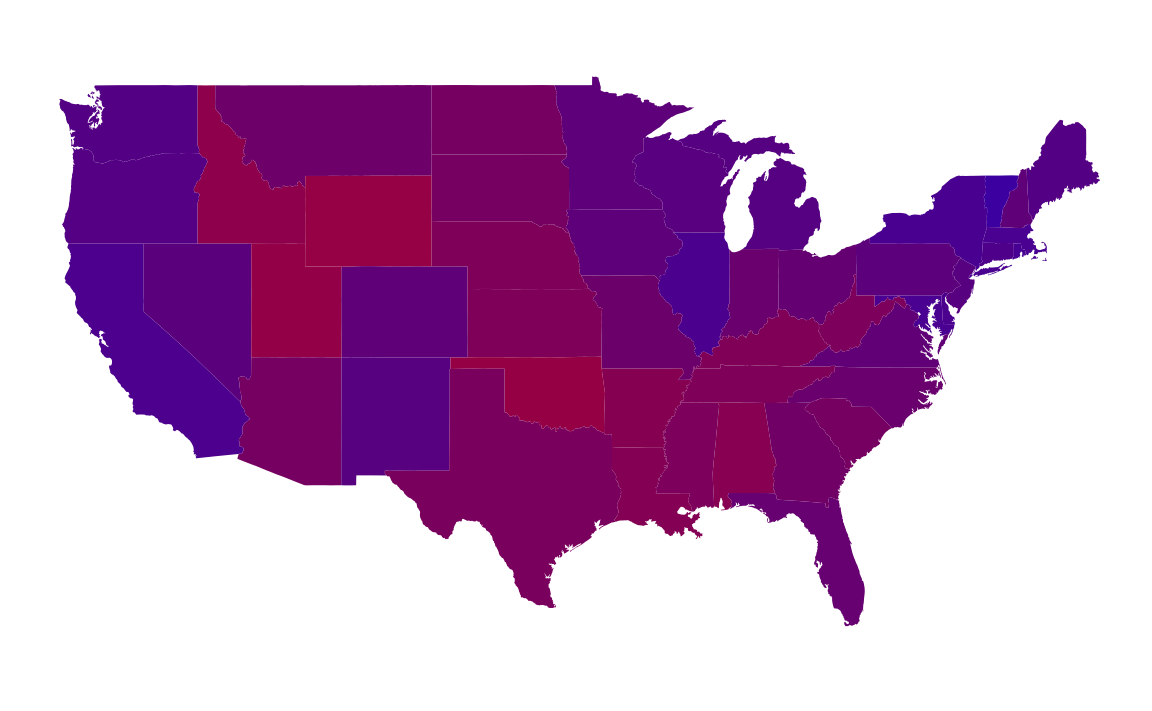
\includegraphics[width=0.7\linewidth]{prediction_files/figure-latex/unnamed-chunk-74-1} \end{center}

See
\href{http://r4ds.had.co.nz/graphics-for-communication.html\#label}{Graphics
for communication} in \emph{R for Data Science} on labels and
annotations in plots.

\hypertarget{regression-and-causation}{%
\section{Regression and Causation}\label{regression-and-causation}}

\hypertarget{randomized-experiments}{%
\subsection{Randomized Experiments}\label{randomized-experiments}}

Load data

\begin{Shaded}
\begin{Highlighting}[]
\KeywordTok{data}\NormalTok{(}\StringTok{"women"}\NormalTok{, }\DataTypeTok{package =} \StringTok{"qss"}\NormalTok{)}
\end{Highlighting}
\end{Shaded}

Proportion of female politicians in reserved GP vs.~unreserved GP

\begin{Shaded}
\begin{Highlighting}[]
\NormalTok{women }\OperatorTok
\StringTok{  }\KeywordTok{group_by}\NormalTok{(reserved) }\OperatorTok
\StringTok{  }\KeywordTok{summarise}\NormalTok{(}\DataTypeTok{prop_female =} \KeywordTok{mean}\NormalTok{(female))}
\CommentTok{#> # A tibble: 2 x 2}
\CommentTok{#>   reserved prop_female}
\CommentTok{#>      <int>       <dbl>}
\CommentTok{#> 1        0      0.0748}
\CommentTok{#> 2        1      1.00}
\end{Highlighting}
\end{Shaded}

The diff in means estimator:

\begin{Shaded}
\begin{Highlighting}[]
\CommentTok{# drinking water facilities}

\CommentTok{# irrigation facilities}
\KeywordTok{mean}\NormalTok{(women}\OperatorTok{$}\NormalTok{irrigation[women}\OperatorTok{$}\NormalTok{reserved }\OperatorTok{==}\StringTok{ }\DecValTok{1}\NormalTok{]) }\OperatorTok{-}
\StringTok{    }\KeywordTok{mean}\NormalTok{(women}\OperatorTok{$}\NormalTok{irrigation[women}\OperatorTok{$}\NormalTok{reserved }\OperatorTok{==}\StringTok{ }\DecValTok{0}\NormalTok{])}
\CommentTok{#> [1] -0.369}
\end{Highlighting}
\end{Shaded}

Mean values of \texttt{irrigation} and \texttt{water} in reserved and
non-reserved districts.

\begin{Shaded}
\begin{Highlighting}[]
\NormalTok{women }\OperatorTok
\StringTok{  }\KeywordTok{group_by}\NormalTok{(reserved) }\OperatorTok
\StringTok{  }\KeywordTok{summarise}\NormalTok{(}\DataTypeTok{irrigation =} \KeywordTok{mean}\NormalTok{(irrigation),}
            \DataTypeTok{water =} \KeywordTok{mean}\NormalTok{(water))}
\CommentTok{#> # A tibble: 2 x 3}
\CommentTok{#>   reserved irrigation water}
\CommentTok{#>      <int>      <dbl> <dbl>}
\CommentTok{#> 1        0       3.39  14.7}
\CommentTok{#> 2        1       3.02  24.0}
\end{Highlighting}
\end{Shaded}

The difference between the two groups can be calculated with the
function
\href{https://www.rdocumentation.org/packages/base/topics/diff}{diff},
which calculates the difference between subsequent observations. This
works as long as we are careful about which group is first or second.

\begin{Shaded}
\begin{Highlighting}[]
\NormalTok{women }\OperatorTok
\StringTok{  }\KeywordTok{group_by}\NormalTok{(reserved) }\OperatorTok
\StringTok{  }\KeywordTok{summarise}\NormalTok{(}\DataTypeTok{irrigation =} \KeywordTok{mean}\NormalTok{(irrigation),}
            \DataTypeTok{water =} \KeywordTok{mean}\NormalTok{(water)) }\OperatorTok
\StringTok{  }\KeywordTok{summarise}\NormalTok{(}\DataTypeTok{diff_irrigation =} \KeywordTok{diff}\NormalTok{(irrigation),}
            \DataTypeTok{diff_water =} \KeywordTok{diff}\NormalTok{(water))}
\CommentTok{#> # A tibble: 1 x 2}
\CommentTok{#>   diff_irrigation diff_water}
\CommentTok{#>             <dbl>      <dbl>}
\CommentTok{#> 1          -0.369       9.25}
\end{Highlighting}
\end{Shaded}

The other way uses \textbf{tidyr}
\href{https://www.rdocumentation.org/packages/tidyr/topics/spread.lm}{spread}
and
\href{https://www.rdocumentation.org/packages/tidyr/topics/gather.lm}{gather},

\begin{Shaded}
\begin{Highlighting}[]
\NormalTok{women }\OperatorTok
\StringTok{  }\KeywordTok{group_by}\NormalTok{(reserved) }\OperatorTok
\StringTok{  }\KeywordTok{summarise}\NormalTok{(}\DataTypeTok{irrigation =} \KeywordTok{mean}\NormalTok{(irrigation),}
            \DataTypeTok{water =} \KeywordTok{mean}\NormalTok{(water)) }\OperatorTok
\StringTok{  }\KeywordTok{gather}\NormalTok{(variable, value, }\OperatorTok{-}\NormalTok{reserved) }\OperatorTok
\StringTok{  }\KeywordTok{spread}\NormalTok{(reserved, value) }\OperatorTok
\StringTok{  }\KeywordTok{mutate}\NormalTok{(}\DataTypeTok{diff =} \StringTok{`}\DataTypeTok{1}\StringTok{`} \OperatorTok{-}\StringTok{ `}\DataTypeTok{0}\StringTok{`}\NormalTok{)}
\CommentTok{#> # A tibble: 2 x 4}
\CommentTok{#>   variable     `0`   `1`   diff}
\CommentTok{#>   <chr>      <dbl> <dbl>  <dbl>}
\CommentTok{#> 1 irrigation  3.39  3.02 -0.369}
\CommentTok{#> 2 water      14.7  24.0   9.25}
\end{Highlighting}
\end{Shaded}

Now each row is an outcome variable of interest, and there are columns
for the treatment (\texttt{1}) and control (\texttt{0}) groups, and the
difference (\texttt{diff}).

\begin{Shaded}
\begin{Highlighting}[]
\KeywordTok{lm}\NormalTok{(water }\OperatorTok{~}\StringTok{ }\NormalTok{reserved, }\DataTypeTok{data =}\NormalTok{ women)}
\CommentTok{#> }
\CommentTok{#> Call:}
\CommentTok{#> lm(formula = water ~ reserved, data = women)}
\CommentTok{#> }
\CommentTok{#> Coefficients:}
\CommentTok{#> (Intercept)     reserved  }
\CommentTok{#>       14.74         9.25}
\end{Highlighting}
\end{Shaded}

\begin{Shaded}
\begin{Highlighting}[]
\KeywordTok{lm}\NormalTok{(irrigation }\OperatorTok{~}\StringTok{ }\NormalTok{reserved, }\DataTypeTok{data =}\NormalTok{ women)}
\CommentTok{#> }
\CommentTok{#> Call:}
\CommentTok{#> lm(formula = irrigation ~ reserved, data = women)}
\CommentTok{#> }
\CommentTok{#> Coefficients:}
\CommentTok{#> (Intercept)     reserved  }
\CommentTok{#>       3.388       -0.369}
\end{Highlighting}
\end{Shaded}

\hypertarget{regression-with-multiple-predictors}{%
\subsection{Regression with multiple
predictors}\label{regression-with-multiple-predictors}}

\begin{Shaded}
\begin{Highlighting}[]
\KeywordTok{data}\NormalTok{(}\StringTok{"social"}\NormalTok{, }\DataTypeTok{package =} \StringTok{"qss"}\NormalTok{)}
\KeywordTok{glimpse}\NormalTok{(social)}
\CommentTok{#> Observations: 305,866}
\CommentTok{#> Variables: 6}
\CommentTok{#> $ sex         <chr> "male", "female", "male", "female", "female", "mal...}
\CommentTok{#> $ yearofbirth <int> 1941, 1947, 1951, 1950, 1982, 1981, 1959, 1956, 19...}
\CommentTok{#> $ primary2004 <int> 0, 0, 0, 0, 0, 0, 0, 0, 0, 0, 1, 0, 0, 1, 1, 1, 0,...}
\CommentTok{#> $ messages    <chr> "Civic Duty", "Civic Duty", "Hawthorne", "Hawthorn...}
\CommentTok{#> $ primary2006 <int> 0, 0, 1, 1, 1, 0, 1, 1, 0, 0, 1, 0, 1, 0, 1, 1, 1,...}
\CommentTok{#> $ hhsize      <int> 2, 2, 3, 3, 3, 3, 3, 3, 2, 2, 1, 2, 2, 1, 2, 2, 1,...}
\KeywordTok{levels}\NormalTok{(social}\OperatorTok{$}\NormalTok{messages)}
\CommentTok{#> NULL}
\NormalTok{fit <-}\StringTok{ }\KeywordTok{lm}\NormalTok{(primary2006 }\OperatorTok{~}\StringTok{ }\NormalTok{messages, }\DataTypeTok{data =}\NormalTok{ social)}
\NormalTok{fit}
\CommentTok{#> }
\CommentTok{#> Call:}
\CommentTok{#> lm(formula = primary2006 ~ messages, data = social)}
\CommentTok{#> }
\CommentTok{#> Coefficients:}
\CommentTok{#>       (Intercept)    messagesControl  messagesHawthorne  }
\CommentTok{#>           0.31454           -0.01790            0.00784  }
\CommentTok{#> messagesNeighbors  }
\CommentTok{#>           0.06341}
\end{Highlighting}
\end{Shaded}

Create indicator variables for each message:

\begin{Shaded}
\begin{Highlighting}[]
\NormalTok{social <-}
\StringTok{  }\NormalTok{social }\OperatorTok
\StringTok{  }\KeywordTok{mutate}\NormalTok{(}\DataTypeTok{Control =} \KeywordTok{as.integer}\NormalTok{(messages }\OperatorTok{==}\StringTok{ "Control"}\NormalTok{),}
         \DataTypeTok{Hawthorne =} \KeywordTok{as.integer}\NormalTok{(messages }\OperatorTok{==}\StringTok{ "Hawthorne"}\NormalTok{),}
         \DataTypeTok{Neighbors =} \KeywordTok{as.integer}\NormalTok{(messages }\OperatorTok{==}\StringTok{ "Neighbors"}\NormalTok{))}
\end{Highlighting}
\end{Shaded}

alternatively, create these using a for loop. This is easier to
understand and less prone to typos:

\begin{Shaded}
\begin{Highlighting}[]
\ControlFlowTok{for}\NormalTok{ (i }\ControlFlowTok{in} \KeywordTok{unique}\NormalTok{(social}\OperatorTok{$}\NormalTok{messages)) \{}
\NormalTok{  social[[i]] <-}\StringTok{ }\KeywordTok{as.integer}\NormalTok{(social[[}\StringTok{"messages"}\NormalTok{]] }\OperatorTok{==}\StringTok{ }\NormalTok{i)}
\NormalTok{\}}
\end{Highlighting}
\end{Shaded}

We created a variable for each level of \texttt{messages} even though we
will exclude one of them.

\begin{Shaded}
\begin{Highlighting}[]
\KeywordTok{lm}\NormalTok{(primary2006 }\OperatorTok{~}\StringTok{ }\NormalTok{Control }\OperatorTok{+}\StringTok{ }\NormalTok{Hawthorne }\OperatorTok{+}\StringTok{ }\NormalTok{Neighbors, }\DataTypeTok{data =}\NormalTok{ social)}
\CommentTok{#> }
\CommentTok{#> Call:}
\CommentTok{#> lm(formula = primary2006 ~ Control + Hawthorne + Neighbors, data = social)}
\CommentTok{#> }
\CommentTok{#> Coefficients:}
\CommentTok{#> (Intercept)      Control    Hawthorne    Neighbors  }
\CommentTok{#>     0.31454     -0.01790      0.00784      0.06341}
\end{Highlighting}
\end{Shaded}

Create predictions for each unique value of \texttt{messages}

\begin{Shaded}
\begin{Highlighting}[]
\NormalTok{unique_messages <-}
\StringTok{  }\KeywordTok{data_grid}\NormalTok{(social, messages) }\OperatorTok
\StringTok{  }\KeywordTok{add_predictions}\NormalTok{(fit)}
\NormalTok{unique_messages}
\CommentTok{#> # A tibble: 4 x 2}
\CommentTok{#>   messages    pred}
\CommentTok{#>   <chr>      <dbl>}
\CommentTok{#> 1 Civic Duty 0.315}
\CommentTok{#> 2 Control    0.297}
\CommentTok{#> 3 Hawthorne  0.322}
\CommentTok{#> 4 Neighbors  0.378}
\end{Highlighting}
\end{Shaded}

Compare to the sample averages

\begin{Shaded}
\begin{Highlighting}[]
\NormalTok{social }\OperatorTok
\StringTok{  }\KeywordTok{group_by}\NormalTok{(messages) }\OperatorTok
\StringTok{  }\KeywordTok{summarise}\NormalTok{(}\KeywordTok{mean}\NormalTok{(primary2006))}
\CommentTok{#> # A tibble: 4 x 2}
\CommentTok{#>   messages   `mean(primary2006)`}
\CommentTok{#>   <chr>                    <dbl>}
\CommentTok{#> 1 Civic Duty               0.315}
\CommentTok{#> 2 Control                  0.297}
\CommentTok{#> 3 Hawthorne                0.322}
\CommentTok{#> 4 Neighbors                0.378}
\end{Highlighting}
\end{Shaded}

Linear regression without intercept.

\begin{Shaded}
\begin{Highlighting}[]
\NormalTok{fit_noint <-}\StringTok{ }\KeywordTok{lm}\NormalTok{(primary2006 }\OperatorTok{~}\StringTok{ }\DecValTok{-1} \OperatorTok{+}\StringTok{ }\NormalTok{messages, }\DataTypeTok{data =}\NormalTok{ social)}
\NormalTok{fit_noint}
\CommentTok{#> }
\CommentTok{#> Call:}
\CommentTok{#> lm(formula = primary2006 ~ -1 + messages, data = social)}
\CommentTok{#> }
\CommentTok{#> Coefficients:}
\CommentTok{#> messagesCivic Duty     messagesControl   messagesHawthorne  }
\CommentTok{#>              0.315               0.297               0.322  }
\CommentTok{#>  messagesNeighbors  }
\CommentTok{#>              0.378}
\end{Highlighting}
\end{Shaded}

Calculating the regression average effect is also easier if we make the
control group the first level so all regression coefficients are
comparisons to it. Use
\href{https://www.rdocumentation.org/packages/forcats/topics/fct_relevel}{fct\_relevel}
to make ``Control''

\begin{Shaded}
\begin{Highlighting}[]
\NormalTok{fit_control <-}
\StringTok{  }\KeywordTok{mutate}\NormalTok{(social, }\DataTypeTok{messages =} \KeywordTok{fct_relevel}\NormalTok{(messages, }\StringTok{"Control"}\NormalTok{)) }\OperatorTok
\StringTok{  }\KeywordTok{lm}\NormalTok{(primary2006 }\OperatorTok{~}\StringTok{ }\NormalTok{messages, }\DataTypeTok{data =}\NormalTok{ .)}
\NormalTok{fit_control}
\CommentTok{#> }
\CommentTok{#> Call:}
\CommentTok{#> lm(formula = primary2006 ~ messages, data = .)}
\CommentTok{#> }
\CommentTok{#> Coefficients:}
\CommentTok{#>        (Intercept)  messagesCivic Duty   messagesHawthorne  }
\CommentTok{#>             0.2966              0.0179              0.0257  }
\CommentTok{#>  messagesNeighbors  }
\CommentTok{#>             0.0813}
\end{Highlighting}
\end{Shaded}

Difference in means

\begin{Shaded}
\begin{Highlighting}[]
\NormalTok{social }\OperatorTok
\StringTok{  }\KeywordTok{group_by}\NormalTok{(messages) }\OperatorTok
\StringTok{  }\KeywordTok{summarise}\NormalTok{(}\DataTypeTok{primary2006 =} \KeywordTok{mean}\NormalTok{(primary2006)) }\OperatorTok
\StringTok{  }\KeywordTok{mutate}\NormalTok{(}\DataTypeTok{Control =}\NormalTok{ primary2006[messages }\OperatorTok{==}\StringTok{ "Control"}\NormalTok{],}
         \DataTypeTok{diff =}\NormalTok{ primary2006 }\OperatorTok{-}\StringTok{ }\NormalTok{Control)}
\CommentTok{#> # A tibble: 4 x 4}
\CommentTok{#>   messages   primary2006 Control   diff}
\CommentTok{#>   <chr>            <dbl>   <dbl>  <dbl>}
\CommentTok{#> 1 Civic Duty       0.315   0.297 0.0179}
\CommentTok{#> 2 Control          0.297   0.297 0.    }
\CommentTok{#> 3 Hawthorne        0.322   0.297 0.0257}
\CommentTok{#> 4 Neighbors        0.378   0.297 0.0813}
\end{Highlighting}
\end{Shaded}

Adjusted R-squared is included in the output of \texttt{broom::glance()}

\begin{Shaded}
\begin{Highlighting}[]
\KeywordTok{glance}\NormalTok{(fit)}
\CommentTok{#>   r.squared adj.r.squared sigma statistic   p.value df  logLik    AIC}
\CommentTok{#> 1   0.00328       0.00327 0.463       336 1.06e-217  4 -198247 396504}
\CommentTok{#>      BIC deviance df.residual}
\CommentTok{#> 1 396557    65468      305862}
\KeywordTok{glance}\NormalTok{(fit)[[}\StringTok{"adj.r.squared"}\NormalTok{]]}
\CommentTok{#> [1] 0.00327}
\end{Highlighting}
\end{Shaded}

\hypertarget{heterogeneous-treatment-effects}{%
\subsection{Heterogeneous Treatment
Effects}\label{heterogeneous-treatment-effects}}

Average treatment effect (ate) among those who voted in 2004 primary

\begin{Shaded}
\begin{Highlighting}[]
\NormalTok{ate <-}
\StringTok{  }\NormalTok{social }\OperatorTok
\StringTok{  }\KeywordTok{group_by}\NormalTok{(primary2004, messages) }\OperatorTok
\StringTok{  }\KeywordTok{summarise}\NormalTok{(}\DataTypeTok{primary2006 =} \KeywordTok{mean}\NormalTok{(primary2006)) }\OperatorTok
\StringTok{  }\KeywordTok{spread}\NormalTok{(messages, primary2006) }\OperatorTok
\StringTok{  }\KeywordTok{mutate}\NormalTok{(}\DataTypeTok{ate_Neighbors =}\NormalTok{ Neighbors }\OperatorTok{-}\StringTok{ }\NormalTok{Control) }\OperatorTok
\StringTok{  }\KeywordTok{select}\NormalTok{(primary2004, Neighbors, Control, ate_Neighbors)}
\NormalTok{ate}
\CommentTok{#> # A tibble: 2 x 4}
\CommentTok{#> # Groups:   primary2004 [2]}
\CommentTok{#>   primary2004 Neighbors Control ate_Neighbors}
\CommentTok{#>         <int>     <dbl>   <dbl>         <dbl>}
\CommentTok{#> 1           0     0.306   0.237        0.0693}
\CommentTok{#> 2           1     0.482   0.386        0.0965}
\end{Highlighting}
\end{Shaded}

Difference in ATE in 2004 voters and non-voters

\begin{Shaded}
\begin{Highlighting}[]
\KeywordTok{diff}\NormalTok{(ate}\OperatorTok{$}\NormalTok{ate_Neighbors)}
\CommentTok{#> [1] 0.0272}
\end{Highlighting}
\end{Shaded}

\begin{Shaded}
\begin{Highlighting}[]
\NormalTok{social_neighbor <-}\StringTok{ }\NormalTok{social }\OperatorTok
\StringTok{  }\KeywordTok{filter}\NormalTok{( (messages }\OperatorTok{==}\StringTok{ "Control"}\NormalTok{) }\OperatorTok{|}\StringTok{ }\NormalTok{(messages }\OperatorTok{==}\StringTok{ "Neighbors"}\NormalTok{))}

\NormalTok{fit_int <-}\StringTok{ }\KeywordTok{lm}\NormalTok{(primary2006 }\OperatorTok{~}\StringTok{ }\NormalTok{primary2004 }\OperatorTok{+}\StringTok{ }\NormalTok{messages }\OperatorTok{+}\StringTok{ }\NormalTok{primary2004}\OperatorTok{:}\NormalTok{messages,}
              \DataTypeTok{data =}\NormalTok{ social_neighbor)}
\NormalTok{fit_int}
\CommentTok{#> }
\CommentTok{#> Call:}
\CommentTok{#> lm(formula = primary2006 ~ primary2004 + messages + primary2004:messages, }
\CommentTok{#>     data = social_neighbor)}
\CommentTok{#> }
\CommentTok{#> Coefficients:}
\CommentTok{#>                   (Intercept)                    primary2004  }
\CommentTok{#>                        0.2371                         0.1487  }
\CommentTok{#>             messagesNeighbors  primary2004:messagesNeighbors  }
\CommentTok{#>                        0.0693                         0.0272}
\end{Highlighting}
\end{Shaded}

\begin{Shaded}
\begin{Highlighting}[]
\KeywordTok{lm}\NormalTok{(primary2006 }\OperatorTok{~}\StringTok{ }\NormalTok{primary2004 }\OperatorTok{*}\StringTok{ }\NormalTok{messages, }\DataTypeTok{data =}\NormalTok{ social_neighbor)}
\CommentTok{#> }
\CommentTok{#> Call:}
\CommentTok{#> lm(formula = primary2006 ~ primary2004 * messages, data = social_neighbor)}
\CommentTok{#> }
\CommentTok{#> Coefficients:}
\CommentTok{#>                   (Intercept)                    primary2004  }
\CommentTok{#>                        0.2371                         0.1487  }
\CommentTok{#>             messagesNeighbors  primary2004:messagesNeighbors  }
\CommentTok{#>                        0.0693                         0.0272}
\end{Highlighting}
\end{Shaded}

\begin{Shaded}
\begin{Highlighting}[]
\NormalTok{social_neighbor <-}
\StringTok{  }\NormalTok{social_neighbor }\OperatorTok
\StringTok{  }\KeywordTok{mutate}\NormalTok{(}\DataTypeTok{age =} \DecValTok{2008} \OperatorTok{-}\StringTok{ }\NormalTok{yearofbirth)}

\KeywordTok{summary}\NormalTok{(social_neighbor}\OperatorTok{$}\NormalTok{age)}
\CommentTok{#>    Min. 1st Qu.  Median    Mean 3rd Qu.    Max. }
\CommentTok{#>    22.0    43.0    52.0    51.8    61.0   108.0}

\NormalTok{fit.age <-}\StringTok{ }\KeywordTok{lm}\NormalTok{(primary2006 }\OperatorTok{~}\StringTok{ }\NormalTok{age }\OperatorTok{*}\StringTok{ }\NormalTok{messages, }\DataTypeTok{data =}\NormalTok{ social_neighbor)}
\NormalTok{fit.age}
\CommentTok{#> }
\CommentTok{#> Call:}
\CommentTok{#> lm(formula = primary2006 ~ age * messages, data = social_neighbor)}
\CommentTok{#> }
\CommentTok{#> Coefficients:}
\CommentTok{#>           (Intercept)                    age      messagesNeighbors  }
\CommentTok{#>              0.089477               0.003998               0.048573  }
\CommentTok{#> age:messagesNeighbors  }
\CommentTok{#>              0.000628}
\end{Highlighting}
\end{Shaded}

Calculate average treatment effects

\begin{Shaded}
\begin{Highlighting}[]
\NormalTok{ate.age <-}
\StringTok{  }\KeywordTok{crossing}\NormalTok{(}\DataTypeTok{age =} \KeywordTok{seq}\NormalTok{(}\DataTypeTok{from =} \DecValTok{25}\NormalTok{, }\DataTypeTok{to =} \DecValTok{85}\NormalTok{, }\DataTypeTok{by =} \DecValTok{20}\NormalTok{),}
         \DataTypeTok{messages =} \KeywordTok{c}\NormalTok{(}\StringTok{"Neighbors"}\NormalTok{, }\StringTok{"Control"}\NormalTok{)) }\OperatorTok
\StringTok{  }\KeywordTok{add_predictions}\NormalTok{(fit.age) }\OperatorTok
\StringTok{  }\KeywordTok{spread}\NormalTok{(messages, pred) }\OperatorTok
\StringTok{  }\KeywordTok{mutate}\NormalTok{(}\DataTypeTok{diff =}\NormalTok{ Neighbors }\OperatorTok{-}\StringTok{ }\NormalTok{Control)}
\NormalTok{ate.age}
\CommentTok{#> # A tibble: 4 x 4}
\CommentTok{#>     age Control Neighbors   diff}
\CommentTok{#>   <dbl>   <dbl>     <dbl>  <dbl>}
\CommentTok{#> 1   25.   0.189     0.254 0.0643}
\CommentTok{#> 2   45.   0.269     0.346 0.0768}
\CommentTok{#> 3   65.   0.349     0.439 0.0894}
\CommentTok{#> 4   85.   0.429     0.531 0.102}
\end{Highlighting}
\end{Shaded}

You can use
\href{https://www.rdocumentation.org/packages/base/topics/poly}{poly}
function to calculate polynomials instead of adding each term,
\texttt{age\ +\ I(age\ \^{}\ 2)}. Though note that the coefficients will
be be different since by default \texttt{poly} calculates orthogonal
polynomials instead of the natural (raw) polynomials. However, you
really shouldn't interpret the coefficients directly anyways, so this
should matter.

\begin{Shaded}
\begin{Highlighting}[]
\NormalTok{fit.age2 <-}\StringTok{ }\KeywordTok{lm}\NormalTok{(primary2006 }\OperatorTok{~}\StringTok{ }\KeywordTok{poly}\NormalTok{(age, }\DecValTok{2}\NormalTok{) }\OperatorTok{*}\StringTok{ }\NormalTok{messages,}
               \DataTypeTok{data =}\NormalTok{ social_neighbor)}
\NormalTok{fit.age2}
\CommentTok{#> }
\CommentTok{#> Call:}
\CommentTok{#> lm(formula = primary2006 ~ poly(age, 2) * messages, data = social_neighbor)}
\CommentTok{#> }
\CommentTok{#> Coefficients:}
\CommentTok{#>                     (Intercept)                    poly(age, 2)1  }
\CommentTok{#>                          0.2966                          27.6665  }
\CommentTok{#>                   poly(age, 2)2                messagesNeighbors  }
\CommentTok{#>                        -10.2832                           0.0816  }
\CommentTok{#> poly(age, 2)1:messagesNeighbors  poly(age, 2)2:messagesNeighbors  }
\CommentTok{#>                          4.5820                          -5.5124}
\end{Highlighting}
\end{Shaded}

Create a data frame of combinations of ages and messages using
\href{https://www.rdocumentation.org/packages/modelr/topics/data_grid}{data\_grid},
which means that we only need to specify the variables, and not the
specific values,

\begin{Shaded}
\begin{Highlighting}[]
\NormalTok{y.hat <-}
\StringTok{  }\KeywordTok{data_grid}\NormalTok{(social_neighbor, age, messages) }\OperatorTok
\StringTok{  }\KeywordTok{add_predictions}\NormalTok{(fit.age2)}
\end{Highlighting}
\end{Shaded}

\begin{Shaded}
\begin{Highlighting}[]
\KeywordTok{ggplot}\NormalTok{(y.hat, }\KeywordTok{aes}\NormalTok{(}\DataTypeTok{x =}\NormalTok{ age, }\DataTypeTok{y =}\NormalTok{ pred,}
                  \DataTypeTok{colour =} \KeywordTok{str_c}\NormalTok{(messages, }\StringTok{" condition"}\NormalTok{))) }\OperatorTok{+}
\StringTok{  }\KeywordTok{geom_line}\NormalTok{() }\OperatorTok{+}
\StringTok{  }\KeywordTok{labs}\NormalTok{(}\DataTypeTok{colour =} \StringTok{""}\NormalTok{, }\DataTypeTok{y =} \StringTok{"Predicted turnout rates"}\NormalTok{) }\OperatorTok{+}
\StringTok{  }\KeywordTok{theme}\NormalTok{(}\DataTypeTok{legend.position =} \StringTok{"bottom"}\NormalTok{)}
\end{Highlighting}
\end{Shaded}

\begin{center}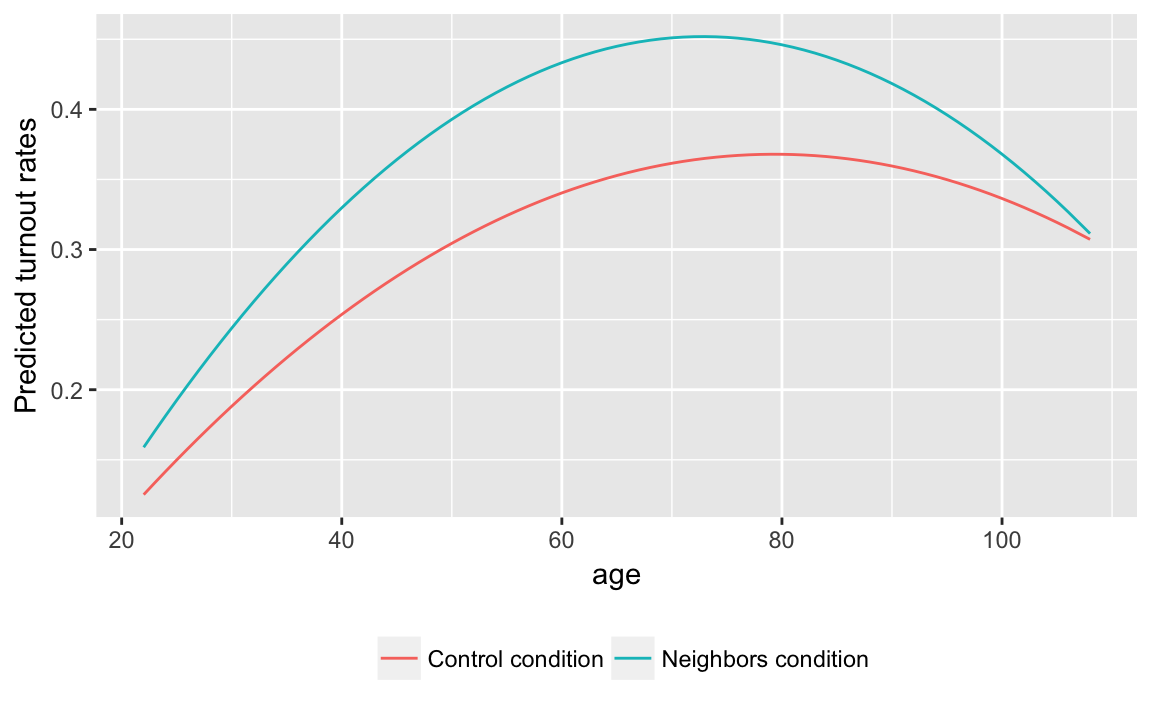
\includegraphics[width=0.7\linewidth]{prediction_files/figure-latex/unnamed-chunk-101-1} \end{center}

\begin{Shaded}
\begin{Highlighting}[]
\NormalTok{y.hat }\OperatorTok
\StringTok{  }\KeywordTok{spread}\NormalTok{(messages, pred) }\OperatorTok
\StringTok{  }\KeywordTok{mutate}\NormalTok{(}\DataTypeTok{ate =}\NormalTok{ Neighbors }\OperatorTok{-}\StringTok{ }\NormalTok{Control) }\OperatorTok
\StringTok{  }\KeywordTok{filter}\NormalTok{(age }\OperatorTok{>}\StringTok{ }\DecValTok{20}\NormalTok{, age }\OperatorTok{<}\StringTok{ }\DecValTok{90}\NormalTok{) }\OperatorTok
\StringTok{  }\KeywordTok{ggplot}\NormalTok{(}\KeywordTok{aes}\NormalTok{(}\DataTypeTok{x =}\NormalTok{ age, }\DataTypeTok{y =}\NormalTok{ ate)) }\OperatorTok{+}
\StringTok{  }\KeywordTok{geom_line}\NormalTok{() }\OperatorTok{+}
\StringTok{  }\KeywordTok{labs}\NormalTok{(}\DataTypeTok{y =} \StringTok{"Estimated average treatment effect"}\NormalTok{,}
       \DataTypeTok{x =} \StringTok{"Age"}\NormalTok{) }\OperatorTok{+}
\StringTok{  }\KeywordTok{ylim}\NormalTok{(}\DecValTok{0}\NormalTok{, }\FloatTok{0.1}\NormalTok{)}
\end{Highlighting}
\end{Shaded}

\begin{center}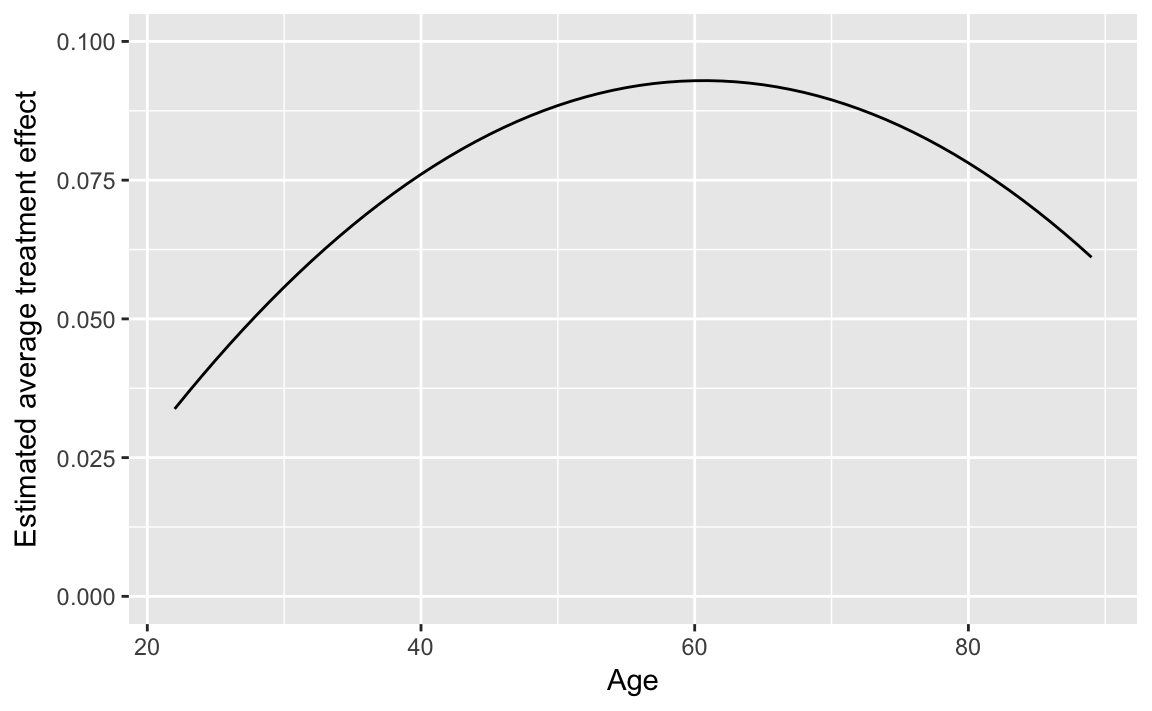
\includegraphics[width=0.7\linewidth]{prediction_files/figure-latex/unnamed-chunk-102-1} \end{center}

\hypertarget{regression-discontinuity-design}{%
\subsection{Regression Discontinuity
Design}\label{regression-discontinuity-design}}

\begin{Shaded}
\begin{Highlighting}[]
\KeywordTok{data}\NormalTok{(}\StringTok{"MPs"}\NormalTok{, }\DataTypeTok{package =} \StringTok{"qss"}\NormalTok{)}

\NormalTok{MPs_labour <-}\StringTok{ }\KeywordTok{filter}\NormalTok{(MPs, party }\OperatorTok{==}\StringTok{ "labour"}\NormalTok{)}
\NormalTok{MPs_tory <-}\StringTok{ }\KeywordTok{filter}\NormalTok{(MPs, party }\OperatorTok{==}\StringTok{ "tory"}\NormalTok{)}

\NormalTok{labour_fit1 <-}\StringTok{ }\KeywordTok{lm}\NormalTok{(ln.net }\OperatorTok{~}\StringTok{ }\NormalTok{margin,}
                 \DataTypeTok{data =} \KeywordTok{filter}\NormalTok{(MPs_labour, margin }\OperatorTok{<}\StringTok{ }\DecValTok{0}\NormalTok{))}
\NormalTok{labour_fit2 <-}\StringTok{ }\KeywordTok{lm}\NormalTok{(ln.net }\OperatorTok{~}\StringTok{ }\NormalTok{margin, MPs_labour, margin }\OperatorTok{>}\StringTok{ }\DecValTok{0}\NormalTok{)}

\NormalTok{tory_fit1 <-}\StringTok{ }\KeywordTok{lm}\NormalTok{(ln.net }\OperatorTok{~}\StringTok{ }\NormalTok{margin,}
                \DataTypeTok{data =} \KeywordTok{filter}\NormalTok{(MPs_tory, margin }\OperatorTok{<}\StringTok{ }\DecValTok{0}\NormalTok{))}
\NormalTok{tory_fit2 <-}\StringTok{ }\KeywordTok{lm}\NormalTok{(ln.net }\OperatorTok{~}\StringTok{ }\NormalTok{margin, }\DataTypeTok{data =} \KeywordTok{filter}\NormalTok{(MPs_tory, margin }\OperatorTok{>}\StringTok{ }\DecValTok{0}\NormalTok{))}
\end{Highlighting}
\end{Shaded}

Use to generate a grid for predictions.

\begin{Shaded}
\begin{Highlighting}[]
\NormalTok{y1_labour <-}
\StringTok{  }\KeywordTok{filter}\NormalTok{(MPs_labour, margin }\OperatorTok{<}\StringTok{ }\DecValTok{0}\NormalTok{) }\OperatorTok
\StringTok{  }\KeywordTok{data_grid}\NormalTok{(margin) }\OperatorTok
\StringTok{  }\KeywordTok{add_predictions}\NormalTok{(labour_fit1)}
\NormalTok{y2_labour <-}
\StringTok{  }\KeywordTok{filter}\NormalTok{(MPs_labour, margin }\OperatorTok{>}\StringTok{ }\DecValTok{0}\NormalTok{) }\OperatorTok
\StringTok{  }\KeywordTok{data_grid}\NormalTok{(margin) }\OperatorTok
\StringTok{  }\KeywordTok{add_predictions}\NormalTok{(labour_fit2)}

\NormalTok{y1_tory <-}
\StringTok{  }\KeywordTok{filter}\NormalTok{(MPs_tory, margin }\OperatorTok{<}\StringTok{ }\DecValTok{0}\NormalTok{) }\OperatorTok
\StringTok{  }\KeywordTok{data_grid}\NormalTok{(margin) }\OperatorTok
\StringTok{  }\KeywordTok{add_predictions}\NormalTok{(tory_fit1)}

\NormalTok{y2_tory <-}
\StringTok{  }\KeywordTok{filter}\NormalTok{(MPs_tory, margin }\OperatorTok{>}\StringTok{ }\DecValTok{0}\NormalTok{) }\OperatorTok
\StringTok{  }\KeywordTok{data_grid}\NormalTok{(margin) }\OperatorTok
\StringTok{  }\KeywordTok{add_predictions}\NormalTok{(tory_fit2)}
\end{Highlighting}
\end{Shaded}

Tory politicians

\begin{Shaded}
\begin{Highlighting}[]
\KeywordTok{ggplot}\NormalTok{() }\OperatorTok{+}
\StringTok{  }\KeywordTok{geom_ref_line}\NormalTok{(}\DataTypeTok{v =} \DecValTok{0}\NormalTok{) }\OperatorTok{+}
\StringTok{  }\KeywordTok{geom_point}\NormalTok{(}\DataTypeTok{data =}\NormalTok{ MPs_tory,}
             \DataTypeTok{mapping =} \KeywordTok{aes}\NormalTok{(}\DataTypeTok{x =}\NormalTok{ margin, }\DataTypeTok{y =}\NormalTok{ ln.net)) }\OperatorTok{+}
\StringTok{  }\KeywordTok{geom_line}\NormalTok{(}\DataTypeTok{data =}\NormalTok{ y1_tory,}
            \DataTypeTok{mapping =} \KeywordTok{aes}\NormalTok{(}\DataTypeTok{x =}\NormalTok{ margin, }\DataTypeTok{y =}\NormalTok{ pred), }\DataTypeTok{colour =} \StringTok{"red"}\NormalTok{, }\DataTypeTok{size =} \FloatTok{1.5}\NormalTok{) }\OperatorTok{+}
\StringTok{  }\KeywordTok{geom_line}\NormalTok{(}\DataTypeTok{data =}\NormalTok{ y2_tory,}
            \DataTypeTok{mapping =} \KeywordTok{aes}\NormalTok{(}\DataTypeTok{x =}\NormalTok{ margin, }\DataTypeTok{y =}\NormalTok{ pred), }\DataTypeTok{colour =} \StringTok{"red"}\NormalTok{, }\DataTypeTok{size =} \FloatTok{1.5}\NormalTok{) }\OperatorTok{+}
\StringTok{  }\KeywordTok{labs}\NormalTok{(}\DataTypeTok{x =} \StringTok{"margin of victory"}\NormalTok{, }\DataTypeTok{y =} \StringTok{"log net wealth at death"}\NormalTok{,}
       \DataTypeTok{title =} \StringTok{"labour"}\NormalTok{)}
\end{Highlighting}
\end{Shaded}

\begin{center}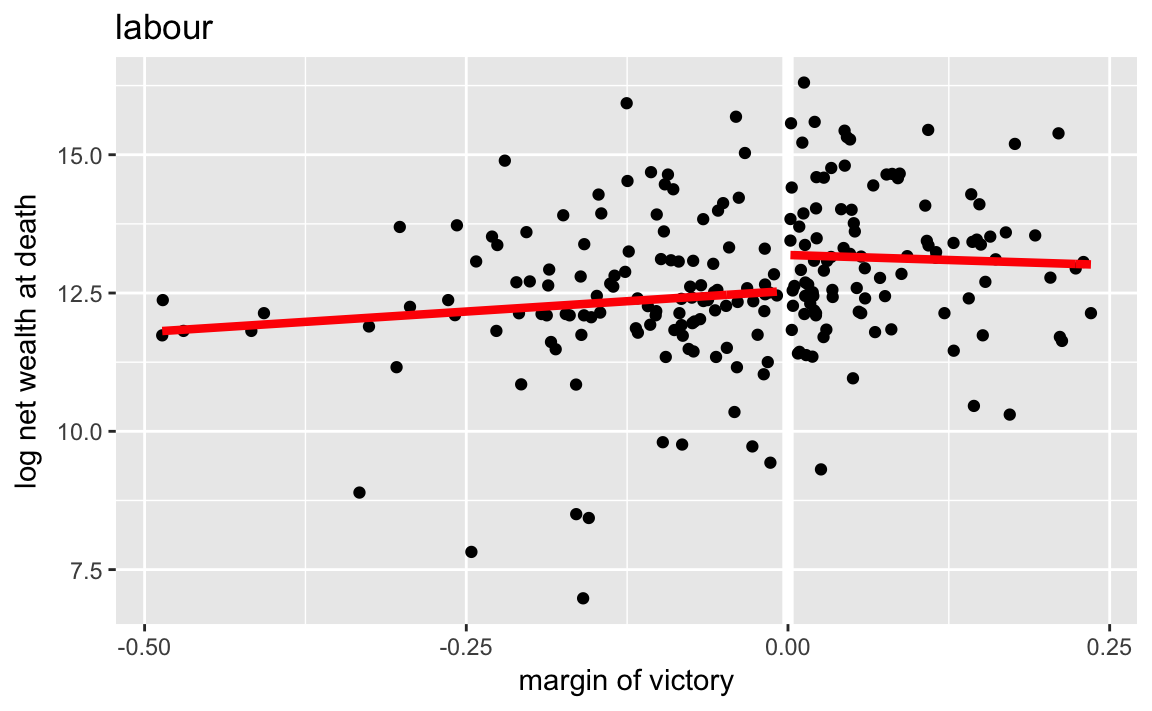
\includegraphics[width=0.7\linewidth]{prediction_files/figure-latex/unnamed-chunk-105-1} \end{center}

We can actually produce this plot easily without running the
regressions, by using \texttt{geom\_smooth}:

\begin{Shaded}
\begin{Highlighting}[]
\KeywordTok{ggplot}\NormalTok{(}\KeywordTok{mutate}\NormalTok{(MPs, }\DataTypeTok{winner =}\NormalTok{ (margin }\OperatorTok{>}\StringTok{ }\DecValTok{0}\NormalTok{)),}
       \KeywordTok{aes}\NormalTok{(}\DataTypeTok{x =}\NormalTok{ margin, }\DataTypeTok{y =}\NormalTok{ ln.net)) }\OperatorTok{+}
\StringTok{  }\KeywordTok{geom_ref_line}\NormalTok{(}\DataTypeTok{v =} \DecValTok{0}\NormalTok{) }\OperatorTok{+}
\StringTok{  }\KeywordTok{geom_point}\NormalTok{() }\OperatorTok{+}
\StringTok{  }\KeywordTok{geom_smooth}\NormalTok{(}\DataTypeTok{method =}\NormalTok{ lm, }\DataTypeTok{se =} \OtherTok{FALSE}\NormalTok{, }\DataTypeTok{mapping =} \KeywordTok{aes}\NormalTok{(}\DataTypeTok{group =}\NormalTok{ winner)) }\OperatorTok{+}
\StringTok{  }\KeywordTok{facet_grid}\NormalTok{(party }\OperatorTok{~}\StringTok{ }\NormalTok{.) }\OperatorTok{+}
\StringTok{  }\KeywordTok{labs}\NormalTok{(}\DataTypeTok{x =} \StringTok{"margin of victory"}\NormalTok{, }\DataTypeTok{y =} \StringTok{"log net wealth at death"}\NormalTok{)}
\end{Highlighting}
\end{Shaded}

\begin{center}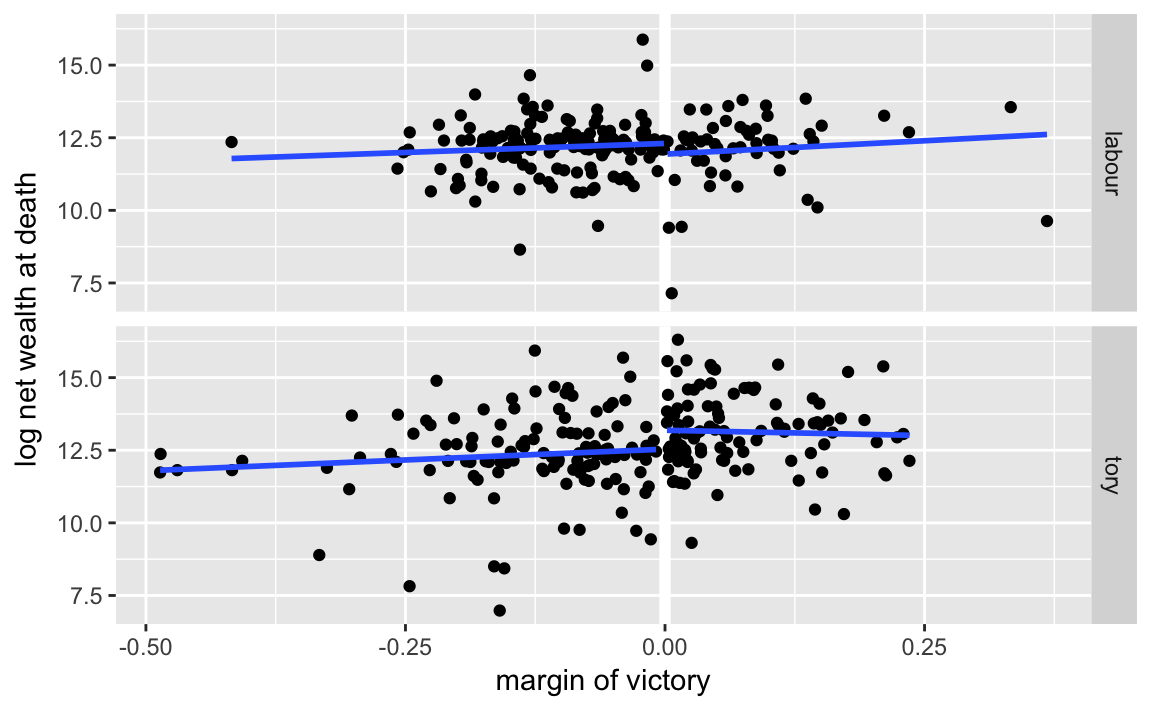
\includegraphics[width=0.7\linewidth]{prediction_files/figure-latex/unnamed-chunk-106-1} \end{center}

In the previous code, I didn't directly compute the the average net
wealth at 0, so I'll need to do that here. I'll use
\href{https://www.rdocumentation.org/packages/modelr/topics/gather_predictions}{gather\_predictions}
to add predictions for multiple models:

\begin{Shaded}
\begin{Highlighting}[]
\KeywordTok{spread_predictions}\NormalTok{(}\KeywordTok{data_frame}\NormalTok{(}\DataTypeTok{margin =} \DecValTok{0}\NormalTok{),}
\NormalTok{                   tory_fit1, tory_fit2) }\OperatorTok
\StringTok{  }\KeywordTok{mutate}\NormalTok{(}\DataTypeTok{rd_est =}\NormalTok{ tory_fit2 }\OperatorTok{-}\StringTok{ }\NormalTok{tory_fit1)}
\CommentTok{#> # A tibble: 1 x 4}
\CommentTok{#>   margin tory_fit1 tory_fit2 rd_est}
\CommentTok{#>    <dbl>     <dbl>     <dbl>  <dbl>}
\CommentTok{#> 1     0.      12.5      13.2  0.650}
\end{Highlighting}
\end{Shaded}

\begin{Shaded}
\begin{Highlighting}[]
\NormalTok{tory_fit3 <-}\StringTok{ }\KeywordTok{lm}\NormalTok{(margin.pre }\OperatorTok{~}\StringTok{ }\NormalTok{margin, }\DataTypeTok{data =} \KeywordTok{filter}\NormalTok{(MPs_tory, margin }\OperatorTok{<}\StringTok{ }\DecValTok{0}\NormalTok{))}
\NormalTok{tory_fit4 <-}\StringTok{ }\KeywordTok{lm}\NormalTok{(margin.pre }\OperatorTok{~}\StringTok{ }\NormalTok{margin, }\DataTypeTok{data =} \KeywordTok{filter}\NormalTok{(MPs_tory, margin }\OperatorTok{>}\StringTok{ }\DecValTok{0}\NormalTok{))}

\NormalTok{(}\KeywordTok{filter}\NormalTok{(}\KeywordTok{tidy}\NormalTok{(tory_fit4), term }\OperatorTok{==}\StringTok{ "(Intercept)"}\NormalTok{)[[}\StringTok{"estimate"}\NormalTok{]] }\OperatorTok{-}
\StringTok{ }\KeywordTok{filter}\NormalTok{(}\KeywordTok{tidy}\NormalTok{(tory_fit3), term }\OperatorTok{==}\StringTok{ "(Intercept)"}\NormalTok{)[[}\StringTok{"estimate"}\NormalTok{]])}
\CommentTok{#> [1] -0.0173}
\end{Highlighting}
\end{Shaded}

\hypertarget{discovery}{%
\chapter{Discovery}\label{discovery}}

The idea of tidy data and the common feature of tidyverse packages is
that data should be stored in data frames with certain conventions. This
works well with naturally tabular data, the type which has been common
in social science applications. But there are other domains in which
other data structures are more appropriate because they more naturally
model the data or processes, or for computational reasons. The three
applications in this chapter: text, networks, and spatial data are
examples where the tidy data structure is less of an advantage. I will
still rely on \textbf{ggplot2} for plotting, and use tidy verse
compatible packages where appropriate.

\begin{itemize}
\tightlist
\item
  Textual data:
  \href{https://cran.r-project.org/package=tidytext}{tidytext}
\item
  Network data: \href{https://cran.r-project.org/package=igraph}{igraph}
  for network computation, as in the chapter. But several
  \textbf{ggplot2}2 extension packages for plotting the networks.
\item
  Spatial data:
  \href{https://cran.r-project.org/package=ggplot2}{ggplot2} has some
  built-in support for maps. The
  \href{https://cran.r-project.org/package=map}{map} package provides
  map data.
\end{itemize}

See the \href{http://r4ds.had.co.nz/}{R for Data Science} section
\href{http://r4ds.had.co.nz/tidy-data.html\#non-tidy-data}{12.7 Non-tidy
data} and this post on
\href{http://simplystatistics.org/2016/02/17/non-tidy-data/}{Non-tidy
data} by Jeff Leek for more on non-tidy data.

\hypertarget{textual-data}{%
\section{Textual data}\label{textual-data}}

\hypertarget{prerequisites-4}{%
\subsection*{Prerequisites}\label{prerequisites-4}}
\addcontentsline{toc}{subsection}{Prerequisites}

\begin{Shaded}
\begin{Highlighting}[]
\KeywordTok{library}\NormalTok{(}\StringTok{"tidyverse"}\NormalTok{)}
\KeywordTok{library}\NormalTok{(}\StringTok{"lubridate"}\NormalTok{)}
\KeywordTok{library}\NormalTok{(}\StringTok{"stringr"}\NormalTok{)}
\KeywordTok{library}\NormalTok{(}\StringTok{"forcats"}\NormalTok{)}
\KeywordTok{library}\NormalTok{(}\StringTok{"modelr"}\NormalTok{)}
\KeywordTok{library}\NormalTok{(}\StringTok{"tm"}\NormalTok{)}
\KeywordTok{library}\NormalTok{(}\StringTok{"SnowballC"}\NormalTok{)}
\KeywordTok{library}\NormalTok{(}\StringTok{"tidytext"}\NormalTok{)}
\KeywordTok{library}\NormalTok{(}\StringTok{"wordcloud"}\NormalTok{)}
\end{Highlighting}
\end{Shaded}

This section will primarily use the
\href{https://cran.r-project.org/package=tidytext}{tidytext} package. It
is a relatively new package. The
\href{https://cran.r-project.org/package=tm}{tm} and
\href{https://cran.r-project.org/package=quanteda}{quanteda} (by Ken
Benoit) packages are more established and use the document-term matrix
format as described in the QSS chapter. The \textbf{tidytext} package
stores everything in a data frame; this may be less efficient than the
other packages, but has the benefit of being able to easily take
advantage of the tidyverse ecosystem. If your corpus is not too large,
this shouldn't be an issue.

See \href{http://tidytextmining.com/}{Tidy Text Mining with R} for a
full introduction to using \textbf{tidytext}.

In tidy data, each row is an observation and each column is a variable.
In the \textbf{tidytext} package, documents are stored as data frames
with \textbf{one-term-per-row}.

We can cast data into the \textbf{tidytext} format either from the
\texttt{Corpus} object, or, after processing, from the document-term
matrix object.

\begin{Shaded}
\begin{Highlighting}[]
\NormalTok{DIR_SOURCE <-}\StringTok{ }\KeywordTok{system.file}\NormalTok{(}\StringTok{"extdata/federalist"}\NormalTok{, }\DataTypeTok{package =} \StringTok{"qss"}\NormalTok{)}
\NormalTok{corpus_raw <-}\StringTok{ }\KeywordTok{VCorpus}\NormalTok{(}\KeywordTok{DirSource}\NormalTok{(}\DataTypeTok{directory =}\NormalTok{ DIR_SOURCE, }\DataTypeTok{pattern =} \StringTok{"fp"}\NormalTok{))}
\NormalTok{corpus_raw}
\CommentTok{#> <<VCorpus>>}
\CommentTok{#> Metadata:  corpus specific: 0, document level (indexed): 0}
\CommentTok{#> Content:  documents: 85}
\end{Highlighting}
\end{Shaded}

Use the function
\href{https://www.rdocumentation.org/packages/tidyytext/topics/tidy.Corpus}{tidy}
to convert the to a data frame with one row per document.

\begin{Shaded}
\begin{Highlighting}[]
\NormalTok{corpus_tidy <-}\StringTok{ }\KeywordTok{tidy}\NormalTok{(corpus_raw, }\StringTok{"corpus"}\NormalTok{)}
\NormalTok{corpus_tidy}
\CommentTok{#> # A tibble: 85 x 8}
\CommentTok{#>   author datetimestamp       description heading id       language origin}
\CommentTok{#>   <lgl>  <dttm>              <lgl>       <lgl>   <chr>    <chr>    <lgl> }
\CommentTok{#> 1 NA     2018-02-26 22:22:03 NA          NA      fp01.txt en       NA    }
\CommentTok{#> 2 NA     2018-02-26 22:22:03 NA          NA      fp02.txt en       NA    }
\CommentTok{#> 3 NA     2018-02-26 22:22:03 NA          NA      fp03.txt en       NA    }
\CommentTok{#> 4 NA     2018-02-26 22:22:03 NA          NA      fp04.txt en       NA    }
\CommentTok{#> 5 NA     2018-02-26 22:22:03 NA          NA      fp05.txt en       NA    }
\CommentTok{#> 6 NA     2018-02-26 22:22:03 NA          NA      fp06.txt en       NA    }
\CommentTok{#> # ... with 79 more rows, and 1 more variable: text <chr>}
\end{Highlighting}
\end{Shaded}

The \texttt{text} column contains the text of the documents themselves.
Since most of the metadata columns are either missings or irrelevant for
our purposes, we'll delete those columns, keeping only the document
(\texttt{id}) and \texttt{text} columns.

\begin{Shaded}
\begin{Highlighting}[]
\NormalTok{corpus_tidy <-}\StringTok{ }\KeywordTok{select}\NormalTok{(corpus_tidy, id, text)}
\end{Highlighting}
\end{Shaded}

Also, we want to extract the essay number and use that as the document
id rather than its file name.

\begin{Shaded}
\begin{Highlighting}[]
\NormalTok{corpus_tidy <-}
\StringTok{  }\KeywordTok{mutate}\NormalTok{(corpus_tidy, }\DataTypeTok{document =} \KeywordTok{as.integer}\NormalTok{(}\KeywordTok{str_extract}\NormalTok{(id, }\StringTok{"}\CharTok{\textbackslash{}\textbackslash{}}\StringTok{d+"}\NormalTok{))) }\OperatorTok
\StringTok{  }\KeywordTok{select}\NormalTok{(}\OperatorTok{-}\NormalTok{id)}
\end{Highlighting}
\end{Shaded}

The function tokenizes the document texts:

\begin{Shaded}
\begin{Highlighting}[]
\NormalTok{tokens <-}\StringTok{ }\NormalTok{corpus_tidy }\OperatorTok
\StringTok{  }\CommentTok{# tokenizes into words and stems them}
\StringTok{  }\KeywordTok{unnest_tokens}\NormalTok{(word, text, }\DataTypeTok{token =} \StringTok{"word_stems"}\NormalTok{) }\OperatorTok
\StringTok{  }\CommentTok{# remove any numbers in the strings}
\StringTok{  }\KeywordTok{mutate}\NormalTok{(}\DataTypeTok{word =} \KeywordTok{str_replace_all}\NormalTok{(word, }\StringTok{"}\CharTok{\textbackslash{}\textbackslash{}}\StringTok{d+"}\NormalTok{, }\StringTok{""}\NormalTok{)) }\OperatorTok
\StringTok{  }\CommentTok{# drop any empty strings}
\StringTok{  }\KeywordTok{filter}\NormalTok{(word }\OperatorTok{!=}\StringTok{ ""}\NormalTok{)}
\NormalTok{tokens}
\CommentTok{#> # A tibble: 202,089 x 2}
\CommentTok{#>   document word     }
\CommentTok{#>      <int> <chr>    }
\CommentTok{#> 1        1 after    }
\CommentTok{#> 2        1 an       }
\CommentTok{#> 3        1 unequivoc}
\CommentTok{#> 4        1 experi   }
\CommentTok{#> 5        1 of       }
\CommentTok{#> 6        1 the      }
\CommentTok{#> # ... with 2.021e+05 more rows}
\end{Highlighting}
\end{Shaded}

The \texttt{unnest\_tokens} function uses the
\href{https://cran.r-project.org/package=tokenizers}{tokenizers} package
to tokenize the text. By default, it uses the function which removes
punctuation, and lowercases the words. I set the tokenizer to to stem
the word, using the
\href{https://cran.r-project.org/package=SnowballC}{SnowballC} package.

We can remove stop-words with an
\href{https://www.rdocumentation.org/packages/dplyr/topics/anti_join}{anti\_join}
on the dataset
\href{https://www.rdocumentation.org/packages/tidytext/topics/stop_words}{stop\_words}

\begin{Shaded}
\begin{Highlighting}[]
\KeywordTok{data}\NormalTok{(}\StringTok{"stop_words"}\NormalTok{, }\DataTypeTok{package =} \StringTok{"tidytext"}\NormalTok{)}
\NormalTok{tokens <-}\StringTok{ }\KeywordTok{anti_join}\NormalTok{(tokens, stop_words, }\DataTypeTok{by =} \StringTok{"word"}\NormalTok{)}
\end{Highlighting}
\end{Shaded}

\hypertarget{document-term-matrix}{%
\subsection{Document-Term Matrix}\label{document-term-matrix}}

In \texttt{tokens} there is one observation for each token (word) in the
each document. This is almost equivalent to a document-term matrix. For
a document-term matrix we need documents, and terms as the keys for the
data and a column with the number of times the term appeared in the
document.

\begin{Shaded}
\begin{Highlighting}[]
\NormalTok{dtm <-}\StringTok{ }\KeywordTok{count}\NormalTok{(tokens, document, word)}
\KeywordTok{head}\NormalTok{(dtm)}
\CommentTok{#> # A tibble: 6 x 3}
\CommentTok{#>   document word           n}
\CommentTok{#>      <int> <chr>      <int>}
\CommentTok{#> 1        1 abl            1}
\CommentTok{#> 2        1 absurd         1}
\CommentTok{#> 3        1 accid          1}
\CommentTok{#> 4        1 accord         1}
\CommentTok{#> 5        1 acknowledg     1}
\CommentTok{#> 6        1 act            1}
\end{Highlighting}
\end{Shaded}

\hypertarget{topic-discovery}{%
\subsection{Topic Discovery}\label{topic-discovery}}

Plot the word-clouds for essays 12 and 24:

\begin{Shaded}
\begin{Highlighting}[]
\KeywordTok{filter}\NormalTok{(dtm, document }\OperatorTok{==}\StringTok{ }\DecValTok{12}\NormalTok{) }\OperatorTok\StringTok{ }\NormalTok{\{}
    \KeywordTok{wordcloud}\NormalTok{(.}\OperatorTok{$}\NormalTok{word, .}\OperatorTok{$}\NormalTok{n, }\DataTypeTok{max.words =} \DecValTok{20}\NormalTok{)}
\NormalTok{  \}}
\end{Highlighting}
\end{Shaded}

\begin{center}\includegraphics[width=0.7\linewidth]{discovery_files/figure-latex/unnamed-chunk-11-1} \end{center}

\begin{Shaded}
\begin{Highlighting}[]
\KeywordTok{filter}\NormalTok{(dtm, document }\OperatorTok{==}\StringTok{ }\DecValTok{24}\NormalTok{) }\OperatorTok\StringTok{ }\NormalTok{\{}
    \KeywordTok{wordcloud}\NormalTok{(.}\OperatorTok{$}\NormalTok{word, .}\OperatorTok{$}\NormalTok{n, }\DataTypeTok{max.words =} \DecValTok{20}\NormalTok{)}
\NormalTok{  \}}
\end{Highlighting}
\end{Shaded}

\begin{center}\includegraphics[width=0.7\linewidth]{discovery_files/figure-latex/unnamed-chunk-12-1} \end{center}

Use the function
\href{https://www.rdocumentation.org/packages/tidytext/topics/bind_tf_idf}{bind\_tf\_idf}
to add a column with the tf-idf to the data frame.

\begin{Shaded}
\begin{Highlighting}[]
\NormalTok{dtm <-}\StringTok{ }\KeywordTok{bind_tf_idf}\NormalTok{(dtm, word, document, n)}
\NormalTok{dtm}
\CommentTok{#> # A tibble: 38,847 x 6}
\CommentTok{#>   document word           n      tf   idf   tf_idf}
\CommentTok{#>      <int> <chr>      <int>   <dbl> <dbl>    <dbl>}
\CommentTok{#> 1        1 abl            1 0.00145 0.705 0.00102 }
\CommentTok{#> 2        1 absurd         1 0.00145 1.73  0.00251 }
\CommentTok{#> 3        1 accid          1 0.00145 3.75  0.00543 }
\CommentTok{#> 4        1 accord         1 0.00145 0.754 0.00109 }
\CommentTok{#> 5        1 acknowledg     1 0.00145 1.55  0.00225 }
\CommentTok{#> 6        1 act            1 0.00145 0.400 0.000579}
\CommentTok{#> # ... with 3.884e+04 more rows}
\end{Highlighting}
\end{Shaded}

The 10 most important words for Paper No.~12 are

\begin{Shaded}
\begin{Highlighting}[]
\NormalTok{dtm }\OperatorTok
\StringTok{  }\KeywordTok{filter}\NormalTok{(document }\OperatorTok{==}\StringTok{ }\DecValTok{12}\NormalTok{) }\OperatorTok
\StringTok{  }\KeywordTok{top_n}\NormalTok{(}\DecValTok{10}\NormalTok{, tf_idf)}
\CommentTok{#> # A tibble: 10 x 6}
\CommentTok{#>   document word           n      tf   idf  tf_idf}
\CommentTok{#>      <int> <chr>      <int>   <dbl> <dbl>   <dbl>}
\CommentTok{#> 1       12 cent           2 0.00199  4.44 0.00884}
\CommentTok{#> 2       12 coast          3 0.00299  3.75 0.0112 }
\CommentTok{#> 3       12 commerc        8 0.00796  1.11 0.00884}
\CommentTok{#> 4       12 contraband     3 0.00299  4.44 0.0133 }
\CommentTok{#> 5       12 excis          5 0.00498  2.65 0.0132 }
\CommentTok{#> 6       12 gallon         2 0.00199  4.44 0.00884}
\CommentTok{#> # ... with 4 more rows}
\end{Highlighting}
\end{Shaded}

and for Paper No.~24,

\begin{Shaded}
\begin{Highlighting}[]
\NormalTok{dtm }\OperatorTok
\StringTok{  }\KeywordTok{filter}\NormalTok{(document }\OperatorTok{==}\StringTok{ }\DecValTok{24}\NormalTok{) }\OperatorTok
\StringTok{  }\KeywordTok{top_n}\NormalTok{(}\DecValTok{10}\NormalTok{, tf_idf)}
\CommentTok{#> # A tibble: 10 x 6}
\CommentTok{#>   document word         n      tf   idf  tf_idf}
\CommentTok{#>      <int> <chr>    <int>   <dbl> <dbl>   <dbl>}
\CommentTok{#> 1       24 armi         7 0.00858  1.26 0.0108 }
\CommentTok{#> 2       24 arsenal      2 0.00245  3.75 0.00919}
\CommentTok{#> 3       24 dock         3 0.00368  4.44 0.0163 }
\CommentTok{#> 4       24 frontier     3 0.00368  2.83 0.0104 }
\CommentTok{#> 5       24 garrison     6 0.00735  2.83 0.0208 }
\CommentTok{#> 6       24 nearer       2 0.00245  3.34 0.00820}
\CommentTok{#> # ... with 4 more rows}
\end{Highlighting}
\end{Shaded}

The slightly different results from the book are due to tokenization
differences.

Subset those documents known to have been written by Hamilton.

\begin{Shaded}
\begin{Highlighting}[]
\NormalTok{HAMILTON_ESSAYS <-}\StringTok{ }\KeywordTok{c}\NormalTok{(}\DecValTok{1}\NormalTok{, }\DecValTok{6}\OperatorTok{:}\DecValTok{9}\NormalTok{, }\DecValTok{11}\OperatorTok{:}\DecValTok{13}\NormalTok{, }\DecValTok{15}\OperatorTok{:}\DecValTok{17}\NormalTok{, }\DecValTok{21}\OperatorTok{:}\DecValTok{36}\NormalTok{, }\DecValTok{59}\OperatorTok{:}\DecValTok{61}\NormalTok{, }\DecValTok{65}\OperatorTok{:}\DecValTok{85}\NormalTok{)}
\NormalTok{dtm_hamilton <-}\StringTok{ }\KeywordTok{filter}\NormalTok{(dtm, document }\OperatorTok\StringTok{ }\NormalTok{HAMILTON_ESSAYS)}
\end{Highlighting}
\end{Shaded}

The
\href{https://www.rdocumentation.org/packages/stats/topics/kmeans}{kmeans}
function expects the input to be rows for observations and columns for
each variable: in our case that would be documents as rows, and words as
columns, with the tf-idf as the cell values. We could use
\texttt{spread} to do this, but that would be a large matrix.

\begin{Shaded}
\begin{Highlighting}[]
\NormalTok{CLUSTERS <-}\StringTok{ }\DecValTok{4}
\NormalTok{km_out <-}
\StringTok{  }\KeywordTok{kmeans}\NormalTok{(}\KeywordTok{cast_dtm}\NormalTok{(dtm_hamilton, document, word, tf_idf), }\DataTypeTok{centers =}\NormalTok{ CLUSTERS,}
         \DataTypeTok{nstart =} \DecValTok{10}\NormalTok{)}
\NormalTok{km_out}\OperatorTok{$}\NormalTok{iter}
\CommentTok{#> [1] 3}
\end{Highlighting}
\end{Shaded}

Data frame with the unique terms used by Hamilton. I extract these from
the column names of the DTM after \texttt{cast\_dtm} to ensure that the
order is the same as the k-means results.

\begin{Shaded}
\begin{Highlighting}[]
\NormalTok{hamilton_words <-}
\StringTok{  }\KeywordTok{tibble}\NormalTok{(}\DataTypeTok{word =} \KeywordTok{colnames}\NormalTok{(}\KeywordTok{cast_dtm}\NormalTok{(dtm_hamilton, document, word, tf_idf)))}
\end{Highlighting}
\end{Shaded}

The centers of the clusters is a cluster x word matrix. We want to
transpose it and then append columns to \texttt{hamilton\_words} so the
location of each word in the cluster is listed.

\begin{Shaded}
\begin{Highlighting}[]
\KeywordTok{dim}\NormalTok{(km_out}\OperatorTok{$}\NormalTok{centers)}
\CommentTok{#> [1]    4 3850}
\end{Highlighting}
\end{Shaded}

\begin{Shaded}
\begin{Highlighting}[]
\NormalTok{hamilton_words <-}\StringTok{ }\KeywordTok{bind_cols}\NormalTok{(hamilton_words, }\KeywordTok{as_tibble}\NormalTok{(}\KeywordTok{t}\NormalTok{(km_out}\OperatorTok{$}\NormalTok{centers)))}
\NormalTok{hamilton_words}
\CommentTok{#> # A tibble: 3,850 x 5}
\CommentTok{#>   word            `1`      `2`     `3`      `4`}
\CommentTok{#>   <chr>         <dbl>    <dbl>   <dbl>    <dbl>}
\CommentTok{#> 1 abl        0.000939 0.000743 0.      0.      }
\CommentTok{#> 2 absurd     0.       0.000517 0.      0.000882}
\CommentTok{#> 3 accid      0.       0.000202 0.      0.      }
\CommentTok{#> 4 accord     0.       0.000399 0.      0.000852}
\CommentTok{#> 5 acknowledg 0.       0.000388 0.      0.000473}
\CommentTok{#> 6 act        0.       0.000560 0.00176 0.000631}
\CommentTok{#> # ... with 3,844 more rows}
\end{Highlighting}
\end{Shaded}

To find the top 10 words in each centroid, we use \texttt{top\_n} with
\texttt{group\_by}:

\begin{Shaded}
\begin{Highlighting}[]
\NormalTok{top_words_cluster <-}
\StringTok{  }\KeywordTok{gather}\NormalTok{(hamilton_words, cluster, value, }\OperatorTok{-}\NormalTok{word) }\OperatorTok
\StringTok{  }\KeywordTok{group_by}\NormalTok{(cluster) }\OperatorTok
\StringTok{  }\KeywordTok{top_n}\NormalTok{(}\DecValTok{10}\NormalTok{, value)}
\end{Highlighting}
\end{Shaded}

We can print them out using a for loop

\begin{Shaded}
\begin{Highlighting}[]
\ControlFlowTok{for}\NormalTok{ (i }\ControlFlowTok{in} \DecValTok{1}\OperatorTok{:}\NormalTok{CLUSTERS) \{}
  \KeywordTok{cat}\NormalTok{(}\StringTok{"CLUSTER "}\NormalTok{, i, }\StringTok{": "}\NormalTok{,}
      \KeywordTok{str_c}\NormalTok{(}\KeywordTok{filter}\NormalTok{(top_words_cluster, cluster }\OperatorTok{==}\StringTok{ }\NormalTok{i)}\OperatorTok{$}\NormalTok{word, }\DataTypeTok{collapse =} \StringTok{", "}\NormalTok{),}
      \StringTok{"}\CharTok{\textbackslash{}n\textbackslash{}n}\StringTok{"}\NormalTok{)}
\NormalTok{\}}
\CommentTok{#> CLUSTER  1 :  presid, appoint, senat, claus, expir, fill, recess, session, unfound, vacanc }
\CommentTok{#> }
\CommentTok{#> CLUSTER  2 :  offic, presid, tax, land, revenu, armi, militia, senat, taxat, claus }
\CommentTok{#> }
\CommentTok{#> CLUSTER  3 :  sedit, guilt, chief, clemenc, impun, plead, crime, pardon, treason, conniv }
\CommentTok{#> }
\CommentTok{#> CLUSTER  4 :  court, jurisdict, inferior, suprem, trial, tribun, cogniz, juri, impeach, appel}
\end{Highlighting}
\end{Shaded}

This is alternative code that prints out a table:

\begin{Shaded}
\begin{Highlighting}[]
\KeywordTok{gather}\NormalTok{(hamilton_words, cluster, value, }\OperatorTok{-}\NormalTok{word) }\OperatorTok
\StringTok{  }\KeywordTok{group_by}\NormalTok{(cluster) }\OperatorTok
\StringTok{  }\KeywordTok{top_n}\NormalTok{(}\DecValTok{10}\NormalTok{, value) }\OperatorTok
\StringTok{  }\KeywordTok{summarise}\NormalTok{(}\DataTypeTok{top_words =} \KeywordTok{str_c}\NormalTok{(word, }\DataTypeTok{collapse =} \StringTok{", "}\NormalTok{)) }\OperatorTok
\StringTok{  }\NormalTok{knitr}\OperatorTok{::}\KeywordTok{kable}\NormalTok{()}
\end{Highlighting}
\end{Shaded}

\begin{tabular}{l|l}
\hline
cluster & top\_words\\
\hline
1 & presid, appoint, senat, claus, expir, fill, recess, session, unfound, vacanc\\
\hline
2 & offic, presid, tax, land, revenu, armi, militia, senat, taxat, claus\\
\hline
3 & sedit, guilt, chief, clemenc, impun, plead, crime, pardon, treason, conniv\\
\hline
4 & court, jurisdict, inferior, suprem, trial, tribun, cogniz, juri, impeach, appel\\
\hline
\end{tabular}

Or to print out the documents in each cluster,

\begin{Shaded}
\begin{Highlighting}[]
\KeywordTok{enframe}\NormalTok{(km_out}\OperatorTok{$}\NormalTok{cluster, }\StringTok{"document"}\NormalTok{, }\StringTok{"cluster"}\NormalTok{) }\OperatorTok
\StringTok{  }\KeywordTok{group_by}\NormalTok{(cluster) }\OperatorTok
\StringTok{  }\KeywordTok{summarise}\NormalTok{(}\DataTypeTok{documents =} \KeywordTok{str_c}\NormalTok{(document, }\DataTypeTok{collapse =} \StringTok{", "}\NormalTok{)) }\OperatorTok
\StringTok{  }\NormalTok{knitr}\OperatorTok{::}\KeywordTok{kable}\NormalTok{()}
\end{Highlighting}
\end{Shaded}

\begin{tabular}{r|l}
\hline
cluster & documents\\
\hline
1 & 67\\
\hline
2 & 1, 6, 7, 8, 9, 11, 12, 13, 15, 16, 17, 21, 22, 23, 24, 25, 26, 27, 28, 29, 30, 31, 32, 33, 34, 35, 36, 59, 60, 61, 66, 68, 69, 70, 71, 72, 73, 75, 76, 77, 78, 79, 80, 84, 85\\
\hline
3 & 74\\
\hline
4 & 65, 81, 82, 83\\
\hline
\end{tabular}

\hypertarget{authorship-prediction}{%
\subsection{Authorship Prediction}\label{authorship-prediction}}

We'll create a data-frame with the known

\begin{Shaded}
\begin{Highlighting}[]
\NormalTok{MADISON_ESSAYS <-}\StringTok{ }\KeywordTok{c}\NormalTok{(}\DecValTok{10}\NormalTok{, }\DecValTok{14}\NormalTok{, }\DecValTok{37}\OperatorTok{:}\DecValTok{48}\NormalTok{, }\DecValTok{58}\NormalTok{)}
\NormalTok{JAY_ESSAYS <-}\StringTok{ }\KeywordTok{c}\NormalTok{(}\DecValTok{2}\OperatorTok{:}\DecValTok{5}\NormalTok{, }\DecValTok{64}\NormalTok{)}
\NormalTok{known_essays <-}\StringTok{ }\KeywordTok{bind_rows}\NormalTok{(}\KeywordTok{tibble}\NormalTok{(}\DataTypeTok{document =}\NormalTok{ MADISON_ESSAYS,}
                                 \DataTypeTok{author =} \StringTok{"Madison"}\NormalTok{),}
                          \KeywordTok{tibble}\NormalTok{(}\DataTypeTok{document =}\NormalTok{ HAMILTON_ESSAYS,}
                                 \DataTypeTok{author =} \StringTok{"Hamilton"}\NormalTok{),}
                          \KeywordTok{tibble}\NormalTok{(}\DataTypeTok{document =}\NormalTok{ JAY_ESSAYS,}
                                 \DataTypeTok{author =} \StringTok{"Jay"}\NormalTok{))}
\end{Highlighting}
\end{Shaded}

\begin{Shaded}
\begin{Highlighting}[]
\NormalTok{STYLE_WORDS <-}
\StringTok{  }\KeywordTok{tibble}\NormalTok{(}\DataTypeTok{word =} \KeywordTok{c}\NormalTok{(}\StringTok{"although"}\NormalTok{, }\StringTok{"always"}\NormalTok{, }\StringTok{"commonly"}\NormalTok{, }\StringTok{"consequently"}\NormalTok{,}
                  \StringTok{"considerable"}\NormalTok{, }\StringTok{"enough"}\NormalTok{, }\StringTok{"there"}\NormalTok{, }\StringTok{"upon"}\NormalTok{, }\StringTok{"while"}\NormalTok{, }\StringTok{"whilst"}\NormalTok{))}

\NormalTok{hm_tfm <-}
\StringTok{  }\KeywordTok{unnest_tokens}\NormalTok{(corpus_tidy, word, text) }\OperatorTok
\StringTok{  }\KeywordTok{count}\NormalTok{(document, word) }\OperatorTok
\StringTok{  }\CommentTok{# term freq per 1000 words}
\StringTok{  }\KeywordTok{group_by}\NormalTok{(document) }\OperatorTok
\StringTok{  }\KeywordTok{mutate}\NormalTok{(}\DataTypeTok{count =}\NormalTok{ n }\OperatorTok{/}\StringTok{ }\KeywordTok{sum}\NormalTok{(n) }\OperatorTok{*}\StringTok{ }\DecValTok{1000}\NormalTok{) }\OperatorTok
\StringTok{  }\KeywordTok{select}\NormalTok{(}\OperatorTok{-}\NormalTok{n) }\OperatorTok
\StringTok{  }\KeywordTok{inner_join}\NormalTok{(STYLE_WORDS, }\DataTypeTok{by =} \StringTok{"word"}\NormalTok{) }\OperatorTok
\StringTok{  }\CommentTok{# merge known essays}
\StringTok{  }\KeywordTok{left_join}\NormalTok{(known_essays, }\DataTypeTok{by =} \StringTok{"document"}\NormalTok{) }\OperatorTok
\StringTok{  }\CommentTok{# make wide with each word a column}
\StringTok{  }\CommentTok{# fill empty values with 0}
\StringTok{  }\KeywordTok{spread}\NormalTok{(word, count, }\DataTypeTok{fill =} \DecValTok{0}\NormalTok{)}
\end{Highlighting}
\end{Shaded}

Calculate average usage by each author of each word

\begin{Shaded}
\begin{Highlighting}[]
\NormalTok{hm_tfm }\OperatorTok
\StringTok{  }\CommentTok{# remove docs with no author}
\StringTok{  }\KeywordTok{filter}\NormalTok{(}\OperatorTok{!}\KeywordTok{is.na}\NormalTok{(author)) }\OperatorTok
\StringTok{  }\CommentTok{# convert back to long (tidy) format to make it easier to summarize}
\StringTok{  }\KeywordTok{gather}\NormalTok{(word, count, }\OperatorTok{-}\NormalTok{document, }\OperatorTok{-}\NormalTok{author) }\OperatorTok
\StringTok{  }\CommentTok{# calculate averge document word usage by author}
\StringTok{  }\KeywordTok{group_by}\NormalTok{(author, word) }\OperatorTok
\StringTok{  }\KeywordTok{summarise}\NormalTok{(}\DataTypeTok{avg_count =} \KeywordTok{mean}\NormalTok{(count)) }\OperatorTok
\StringTok{  }\KeywordTok{spread}\NormalTok{(author, avg_count) }\OperatorTok
\StringTok{  }\NormalTok{knitr}\OperatorTok{::}\KeywordTok{kable}\NormalTok{()}
\end{Highlighting}
\end{Shaded}

\begin{tabular}{l|r|r|r}
\hline
word & Hamilton & Jay & Madison\\
\hline
although & 0.012 & 0.543 & 0.206\\
\hline
always & 0.522 & 0.929 & 0.154\\
\hline
commonly & 0.184 & 0.129 & 0.000\\
\hline
consequently & 0.018 & 0.469 & 0.344\\
\hline
considerable & 0.377 & 0.081 & 0.123\\
\hline
enough & 0.274 & 0.000 & 0.000\\
\hline
there & 3.065 & 0.954 & 0.849\\
\hline
upon & 3.054 & 0.112 & 0.152\\
\hline
while & 0.255 & 0.192 & 0.000\\
\hline
whilst & 0.005 & 0.000 & 0.292\\
\hline
\end{tabular}

\begin{Shaded}
\begin{Highlighting}[]
\NormalTok{author_data <-}
\StringTok{  }\NormalTok{hm_tfm }\OperatorTok
\StringTok{  }\KeywordTok{ungroup}\NormalTok{() }\OperatorTok
\StringTok{  }\KeywordTok{filter}\NormalTok{(}\KeywordTok{is.na}\NormalTok{(author) }\OperatorTok{|}\StringTok{ }\NormalTok{author }\OperatorTok{!=}\StringTok{ "Jay"}\NormalTok{) }\OperatorTok
\StringTok{  }\KeywordTok{mutate}\NormalTok{(}\DataTypeTok{author2 =} \KeywordTok{case_when}\NormalTok{(.}\OperatorTok{$}\NormalTok{author }\OperatorTok{==}\StringTok{ "Hamilton"} \OperatorTok{~}\StringTok{ }\DecValTok{1}\NormalTok{,}
\NormalTok{                             .}\OperatorTok{$}\NormalTok{author }\OperatorTok{==}\StringTok{ "Madison"} \OperatorTok{~}\StringTok{ }\DecValTok{-1}\NormalTok{,}
                             \OtherTok{TRUE} \OperatorTok{~}\StringTok{ }\OtherTok{NA_real_}\NormalTok{))}

\NormalTok{hm_fit <-}\StringTok{ }\KeywordTok{lm}\NormalTok{(author2 }\OperatorTok{~}\StringTok{ }\NormalTok{upon }\OperatorTok{+}\StringTok{ }\NormalTok{there }\OperatorTok{+}\StringTok{ }\NormalTok{consequently }\OperatorTok{+}\StringTok{ }\NormalTok{whilst,}
             \DataTypeTok{data =}\NormalTok{ author_data)}
\NormalTok{hm_fit}
\CommentTok{#> }
\CommentTok{#> Call:}
\CommentTok{#> lm(formula = author2 ~ upon + there + consequently + whilst, }
\CommentTok{#>     data = author_data)}
\CommentTok{#> }
\CommentTok{#> Coefficients:}
\CommentTok{#>  (Intercept)          upon         there  consequently        whilst  }
\CommentTok{#>       -0.195         0.229         0.127        -0.644        -0.984}

\NormalTok{author_data <-}\StringTok{ }\NormalTok{author_data }\OperatorTok
\StringTok{  }\KeywordTok{add_predictions}\NormalTok{(hm_fit) }\OperatorTok
\StringTok{  }\KeywordTok{mutate}\NormalTok{(}\DataTypeTok{pred_author =} \KeywordTok{if_else}\NormalTok{(pred }\OperatorTok{>=}\StringTok{ }\DecValTok{0}\NormalTok{, }\StringTok{"Hamilton"}\NormalTok{, }\StringTok{"Madison"}\NormalTok{))}

\KeywordTok{sd}\NormalTok{(author_data}\OperatorTok{$}\NormalTok{pred)}
\CommentTok{#> [1] 0.79}
\end{Highlighting}
\end{Shaded}

These coefficients are a little different, probably due to differences
in the tokenization procedure, and in particular, the document size
normalization.

\hypertarget{cross-validation}{%
\subsection{Cross-Validation}\label{cross-validation}}

\textbf{tidyverse:} For cross-validation, I rely on the
\href{https://cran.r-project.org/package=modelr}{modelr} package
function \texttt{RDoc("modelr::crossv\_kfold")}. See the tutorial
\href{https://rpubs.com/dgrtwo/cv-modelr}{Cross validation of linear
regression with modelr} for more on using \textbf{modelr} for cross
validation or
\href{https://drsimonj.svbtle.com/k-fold-cross-validation-with-modelr-and-broom}{k-fold
cross-validation with modelr and broom}.

In sample, this regression perfectly predicts the authorship of the
documents with known authors.

\begin{Shaded}
\begin{Highlighting}[]
\NormalTok{author_data }\OperatorTok
\StringTok{  }\KeywordTok{filter}\NormalTok{(}\OperatorTok{!}\KeywordTok{is.na}\NormalTok{(author)) }\OperatorTok
\StringTok{  }\KeywordTok{group_by}\NormalTok{(author) }\OperatorTok
\StringTok{  }\KeywordTok{summarise}\NormalTok{(}\StringTok{`}\DataTypeTok{Proportion Correct}\StringTok{`}\NormalTok{ =}\StringTok{ }\KeywordTok{mean}\NormalTok{(author }\OperatorTok{==}\StringTok{ }\NormalTok{pred_author))}
\CommentTok{#> # A tibble: 2 x 2}
\CommentTok{#>   author   `Proportion Correct`}
\CommentTok{#>   <chr>                   <dbl>}
\CommentTok{#> 1 Hamilton                   1.}
\CommentTok{#> 2 Madison                    1.}
\end{Highlighting}
\end{Shaded}

Create the cross-validation data-sets using . As in the chapter, I will
use a leave-one-out cross-validation, which is a k-fold cross-validation
where k is the number of observations. To simplify this, I define the
\texttt{crossv\_loo} function that runs \texttt{crossv\_kfold} with
\texttt{k\ =\ nrow(data)}.

\begin{Shaded}
\begin{Highlighting}[]
\NormalTok{crossv_loo <-}\StringTok{ }\ControlFlowTok{function}\NormalTok{(data, }\DataTypeTok{id =} \StringTok{".id"}\NormalTok{) \{}
\NormalTok{  modelr}\OperatorTok{::}\KeywordTok{crossv_kfold}\NormalTok{(data, }\DataTypeTok{k =} \KeywordTok{nrow}\NormalTok{(data), }\DataTypeTok{id =}\NormalTok{ id)}
\NormalTok{\}}

\CommentTok{# leave one out cross-validation object}
\NormalTok{cv <-}\StringTok{ }\NormalTok{author_data }\OperatorTok
\StringTok{  }\KeywordTok{filter}\NormalTok{(}\OperatorTok{!}\KeywordTok{is.na}\NormalTok{(author)) }\OperatorTok
\StringTok{  }\KeywordTok{crossv_loo}\NormalTok{()}
\end{Highlighting}
\end{Shaded}

Now estimate the model for each training dataset

\begin{Shaded}
\begin{Highlighting}[]
\NormalTok{models <-}\StringTok{ }\NormalTok{purrr}\OperatorTok{::}\KeywordTok{map}\NormalTok{(cv}\OperatorTok{$}\NormalTok{train, }\OperatorTok{~}\StringTok{ }\KeywordTok{lm}\NormalTok{(author2 }\OperatorTok{~}\StringTok{ }\NormalTok{upon }\OperatorTok{+}\StringTok{ }\NormalTok{there }\OperatorTok{+}\StringTok{ }\NormalTok{consequently }\OperatorTok{+}\StringTok{ }\NormalTok{whilst,}
                             \DataTypeTok{data =}\NormalTok{ ., }\DataTypeTok{model =} \OtherTok{FALSE}\NormalTok{))}
\end{Highlighting}
\end{Shaded}

Note that I use \texttt{purrr::map} to ensure that the correct
\texttt{map()} function is used since the \textbf{maps} package also
defines a \texttt{map}.

Now calculate the test performance on the held out observation,

\begin{Shaded}
\begin{Highlighting}[]
\NormalTok{test <-}\StringTok{ }\KeywordTok{map2_df}\NormalTok{(models, cv}\OperatorTok{$}\NormalTok{test,}
                \ControlFlowTok{function}\NormalTok{(mod, test) \{}
                  \KeywordTok{add_predictions}\NormalTok{(}\KeywordTok{as.data.frame}\NormalTok{(test), mod) }\OperatorTok
\StringTok{                    }\KeywordTok{mutate}\NormalTok{(}\DataTypeTok{pred_author =}
                             \KeywordTok{if_else}\NormalTok{(pred }\OperatorTok{>=}\StringTok{ }\DecValTok{0}\NormalTok{, }\StringTok{"Hamilton"}\NormalTok{, }\StringTok{"Madison"}\NormalTok{),}
                           \DataTypeTok{correct =}\NormalTok{ (pred_author }\OperatorTok{==}\StringTok{ }\NormalTok{author))}
\NormalTok{                \})}
\NormalTok{test }\OperatorTok
\StringTok{  }\KeywordTok{group_by}\NormalTok{(author) }\OperatorTok
\StringTok{  }\KeywordTok{summarise}\NormalTok{(}\KeywordTok{mean}\NormalTok{(correct))}
\CommentTok{#> # A tibble: 2 x 2}
\CommentTok{#>   author   `mean(correct)`}
\CommentTok{#>   <chr>              <dbl>}
\CommentTok{#> 1 Hamilton           1.00 }
\CommentTok{#> 2 Madison            0.786}
\end{Highlighting}
\end{Shaded}

When adding prediction with \texttt{add\_predictions} it added
predictions for missing values as well.

Table of authorship of disputed papers

\begin{Shaded}
\begin{Highlighting}[]
\NormalTok{author_data }\OperatorTok
\StringTok{  }\KeywordTok{filter}\NormalTok{(}\KeywordTok{is.na}\NormalTok{(author)) }\OperatorTok
\StringTok{  }\KeywordTok{select}\NormalTok{(document, pred, pred_author) }\OperatorTok
\StringTok{  }\NormalTok{knitr}\OperatorTok{::}\KeywordTok{kable}\NormalTok{()}
\end{Highlighting}
\end{Shaded}

\begin{tabular}{r|r|l}
\hline
document & pred & pred\_author\\
\hline
18 & -0.360 & Madison\\
\hline
19 & -0.587 & Madison\\
\hline
20 & -0.055 & Madison\\
\hline
49 & -0.966 & Madison\\
\hline
50 & -0.003 & Madison\\
\hline
51 & -1.520 & Madison\\
\hline
52 & -0.195 & Madison\\
\hline
53 & -0.506 & Madison\\
\hline
54 & -0.521 & Madison\\
\hline
55 & 0.094 & Hamilton\\
\hline
56 & -0.550 & Madison\\
\hline
57 & -1.221 & Madison\\
\hline
62 & -0.946 & Madison\\
\hline
63 & -0.184 & Madison\\
\hline
\end{tabular}

\begin{Shaded}
\begin{Highlighting}[]
\NormalTok{disputed_essays <-}\StringTok{ }\KeywordTok{filter}\NormalTok{(author_data, }\KeywordTok{is.na}\NormalTok{(author))}\OperatorTok{$}\NormalTok{document}

\KeywordTok{ggplot}\NormalTok{(}\KeywordTok{mutate}\NormalTok{(author_data,}
              \DataTypeTok{author =} \KeywordTok{fct_explicit_na}\NormalTok{(}\KeywordTok{factor}\NormalTok{(author), }\StringTok{"Disputed"}\NormalTok{)),}
       \KeywordTok{aes}\NormalTok{(}\DataTypeTok{y =}\NormalTok{ document, }\DataTypeTok{x =}\NormalTok{ pred, }\DataTypeTok{colour =}\NormalTok{ author, }\DataTypeTok{shape =}\NormalTok{ author)) }\OperatorTok{+}
\StringTok{  }\KeywordTok{geom_ref_line}\NormalTok{(}\DataTypeTok{v =} \DecValTok{0}\NormalTok{) }\OperatorTok{+}
\StringTok{  }\KeywordTok{geom_point}\NormalTok{() }\OperatorTok{+}
\StringTok{  }\KeywordTok{scale_y_continuous}\NormalTok{(}\DataTypeTok{breaks =} \KeywordTok{seq}\NormalTok{(}\DecValTok{10}\NormalTok{, }\DecValTok{80}\NormalTok{, }\DataTypeTok{by =} \DecValTok{10}\NormalTok{),}
                     \DataTypeTok{minor_breaks =} \KeywordTok{seq}\NormalTok{(}\DecValTok{5}\NormalTok{, }\DecValTok{80}\NormalTok{, }\DataTypeTok{by =} \DecValTok{5}\NormalTok{)) }\OperatorTok{+}
\StringTok{  }\KeywordTok{scale_color_manual}\NormalTok{(}\DataTypeTok{values =} \KeywordTok{c}\NormalTok{(}\StringTok{"Madison"}\NormalTok{ =}\StringTok{ "blue"}\NormalTok{,}
                                \StringTok{"Hamilton"}\NormalTok{ =}\StringTok{ "red"}\NormalTok{,}
                                \StringTok{"Disputed"}\NormalTok{ =}\StringTok{ "black"}\NormalTok{)) }\OperatorTok{+}
\StringTok{  }\KeywordTok{scale_shape_manual}\NormalTok{(}\DataTypeTok{values =} \KeywordTok{c}\NormalTok{(}\StringTok{"Madison"}\NormalTok{ =}\StringTok{ }\DecValTok{16}\NormalTok{, }\StringTok{"Hamilton"}\NormalTok{ =}\StringTok{ }\DecValTok{15}\NormalTok{,}
                                 \StringTok{"Disputed"}\NormalTok{ =}\StringTok{ }\DecValTok{17}\NormalTok{)) }\OperatorTok{+}
\StringTok{  }\KeywordTok{labs}\NormalTok{(}\DataTypeTok{colour =} \StringTok{"Author"}\NormalTok{, }\DataTypeTok{shape =} \StringTok{"Author"}\NormalTok{,}
       \DataTypeTok{y =} \StringTok{"Federalist Papers"}\NormalTok{, }\DataTypeTok{x =} \StringTok{"Predicted values"}\NormalTok{)}
\end{Highlighting}
\end{Shaded}

\begin{center}\includegraphics[width=0.7\linewidth]{discovery_files/figure-latex/unnamed-chunk-30-1} \end{center}

\hypertarget{network-data}{%
\section{Network data}\label{network-data}}

The \href{https://cran.r-project.org/package=igraph}{igraph},
\href{https://cran.r-project.org/package=sna}{sna}, and
\href{https://cran.r-project.org/package=network}{network} packages are
the best in class. See the Social Network Analysis section of the
\href{https://cran.r-project.org/web/views/SocialSciences.html}{Social
Sciences Task View}. See this tutorial by Katherin Ognyanova,
\href{https://rpubs.com/kateto/netviz}{Static and dynamic network
visualization with R}, for a good overview of network visualization with
those packages in R.

There are several packages that plot networks in ggplot2.

\begin{itemize}
\tightlist
\item
  \href{https://cran.r-project.org/package=ggnetwork}{ggnetwork}
\item
  \href{https://cran.r-project.org/package=ggraph}{ggraph}
\item
  \href{https://cran.r-project.org/package=geomnet}{geomnet}
\item
  \href{https://cran.r-project.org/package=GGally}{GGally} functions
  \href{https://ggobi.github.io/ggally/rd.html\#ggnet}{ggnet},
  \texttt{ggnet2}, and \texttt{ggnetworkmap}.
\item
  \href{https://cran.r-project.org/package=ggCompNet}{ggCompNet}
  compares the speed of various network plotting packages in R.
\end{itemize}

See this
\href{http://curleylab.psych.columbia.edu/netviz/netviz1.html\#/12}{presentation}
for an overview of some of those packages for data visualization.

Examples:
\href{https://cran.r-project.org/web/packages/ggCompNet/vignettes/examples-from-paper.html}{Network
Visualization Examples with the ggplot2 Package}

\hypertarget{prerequisites-5}{%
\subsection*{Prerequisites}\label{prerequisites-5}}
\addcontentsline{toc}{subsection}{Prerequisites}

\begin{Shaded}
\begin{Highlighting}[]
\KeywordTok{library}\NormalTok{(}\StringTok{"tidyverse"}\NormalTok{)}
\KeywordTok{library}\NormalTok{(}\StringTok{"lubridate"}\NormalTok{)}
\KeywordTok{library}\NormalTok{(}\StringTok{"stringr"}\NormalTok{)}
\KeywordTok{library}\NormalTok{(}\StringTok{"forcats"}\NormalTok{)}
\KeywordTok{library}\NormalTok{(}\StringTok{"igraph"}\NormalTok{)}
\KeywordTok{library}\NormalTok{(}\StringTok{"intergraph"}\NormalTok{)}
\KeywordTok{library}\NormalTok{(}\StringTok{"GGally"}\NormalTok{)}
\end{Highlighting}
\end{Shaded}

\hypertarget{twitter-following-network}{%
\subsection{Twitter Following Network}\label{twitter-following-network}}

\begin{Shaded}
\begin{Highlighting}[]
\KeywordTok{data}\NormalTok{(}\StringTok{"twitter.following"}\NormalTok{, }\DataTypeTok{package =} \StringTok{"qss"}\NormalTok{)}
\end{Highlighting}
\end{Shaded}

\begin{Shaded}
\begin{Highlighting}[]
\KeywordTok{data}\NormalTok{(}\StringTok{"twitter.senator"}\NormalTok{, }\DataTypeTok{package =} \StringTok{"qss"}\NormalTok{)}
\end{Highlighting}
\end{Shaded}

Since the names \texttt{twitter.following} and \texttt{twitter.senator}
are verbose, we'll simplify future code by copying their values to
variables named \texttt{twitter} and \texttt{senator}, respectively.

\begin{Shaded}
\begin{Highlighting}[]
\NormalTok{twitter <-}\StringTok{ }\NormalTok{twitter.following}
\NormalTok{senator <-}\StringTok{ }\NormalTok{twitter.senator}
\end{Highlighting}
\end{Shaded}

Simply use the function since \texttt{twitter} consists of edges (a link
from a senator to another). Since \texttt{graph\_from\_edgelist} expects
a matrix, convert the data frame to a matrix using .

\begin{Shaded}
\begin{Highlighting}[]
\NormalTok{twitter_adj <-}\StringTok{ }\KeywordTok{graph_from_edgelist}\NormalTok{(}\KeywordTok{as.matrix}\NormalTok{(twitter))}
\end{Highlighting}
\end{Shaded}

Add in- and out-degree variables to the \texttt{senator} data frame:

\begin{Shaded}
\begin{Highlighting}[]
\NormalTok{senator <-}
\StringTok{  }\KeywordTok{mutate}\NormalTok{(senator,}
         \DataTypeTok{indegree =}\NormalTok{ igraph}\OperatorTok{::}\KeywordTok{degree}\NormalTok{(twitter_adj, }\DataTypeTok{mode =} \StringTok{"in"}\NormalTok{),}
         \DataTypeTok{outdegree =}\NormalTok{ igraph}\OperatorTok{::}\KeywordTok{degree}\NormalTok{(twitter_adj, }\DataTypeTok{mode =} \StringTok{"out"}\NormalTok{))}
\end{Highlighting}
\end{Shaded}

Now find the senators with the 3 greatest in-degrees

\begin{Shaded}
\begin{Highlighting}[]
\KeywordTok{arrange}\NormalTok{(senator, }\KeywordTok{desc}\NormalTok{(indegree)) }\OperatorTok
\StringTok{  }\KeywordTok{slice}\NormalTok{(}\DecValTok{1}\OperatorTok{:}\DecValTok{3}\NormalTok{) }\OperatorTok
\StringTok{  }\KeywordTok{select}\NormalTok{(name, party, state, indegree, outdegree)}
\CommentTok{#> # A tibble: 3 x 5}
\CommentTok{#>   name              party state indegree outdegree}
\CommentTok{#>   <chr>             <chr> <chr>    <dbl>     <dbl>}
\CommentTok{#> 1 Tom Cotton        R     AR         64.       15.}
\CommentTok{#> 2 Richard J. Durbin D     IL         60.       87.}
\CommentTok{#> 3 John Barrasso     R     WY         58.       79.}
\end{Highlighting}
\end{Shaded}

or using the function:

\begin{Shaded}
\begin{Highlighting}[]
\KeywordTok{top_n}\NormalTok{(senator, }\DecValTok{3}\NormalTok{, indegree) }\OperatorTok
\StringTok{  }\KeywordTok{arrange}\NormalTok{(}\KeywordTok{desc}\NormalTok{(indegree)) }\OperatorTok
\StringTok{  }\KeywordTok{select}\NormalTok{(name, party, state, indegree, outdegree)}
\CommentTok{#>                name party state indegree outdegree}
\CommentTok{#> 1        Tom Cotton     R    AR       64        15}
\CommentTok{#> 2 Richard J. Durbin     D    IL       60        87}
\CommentTok{#> 3     John Barrasso     R    WY       58        79}
\CommentTok{#> 4      Joe Donnelly     D    IN       58         9}
\CommentTok{#> 5    Orrin G. Hatch     R    UT       58        50}
\end{Highlighting}
\end{Shaded}

The \texttt{top\_n} function catches that three senators are tied for
3rd highest outdegree, whereas the simply sorting and slicing cannot.

And we can find the senators with the three highest out-degrees
similarly,

\begin{Shaded}
\begin{Highlighting}[]
\KeywordTok{top_n}\NormalTok{(senator, }\DecValTok{3}\NormalTok{, outdegree) }\OperatorTok
\StringTok{  }\KeywordTok{arrange}\NormalTok{(}\KeywordTok{desc}\NormalTok{(outdegree)) }\OperatorTok
\StringTok{  }\KeywordTok{select}\NormalTok{(name, party, state, indegree, outdegree)}
\CommentTok{#>               name party state indegree outdegree}
\CommentTok{#> 1     Thad Cochran     R    MS       55        89}
\CommentTok{#> 2     Steve Daines     R    MT       30        88}
\CommentTok{#> 3      John McCain     R    AZ       41        88}
\CommentTok{#> 4 Joe Manchin, III     D    WV       43        88}
\end{Highlighting}
\end{Shaded}

\begin{Shaded}
\begin{Highlighting}[]
\CommentTok{# Define scales to reuse for the plots}
\NormalTok{scale_colour_parties <-}\StringTok{ }\KeywordTok{scale_colour_manual}\NormalTok{(}\StringTok{"Party"}\NormalTok{, }\DataTypeTok{values =} \KeywordTok{c}\NormalTok{(}\DataTypeTok{R =} \StringTok{"red"}\NormalTok{,}
                                                       \DataTypeTok{D =} \StringTok{"blue"}\NormalTok{,}
                                                       \DataTypeTok{I =} \StringTok{"green"}\NormalTok{))}
\NormalTok{scale_shape_parties <-}\StringTok{ }\KeywordTok{scale_shape_manual}\NormalTok{(}\StringTok{"Party"}\NormalTok{, }\DataTypeTok{values =} \KeywordTok{c}\NormalTok{(}\DataTypeTok{R =} \DecValTok{16}\NormalTok{,}
                                                              \DataTypeTok{D =} \DecValTok{17}\NormalTok{,}
                                                              \DataTypeTok{I =} \DecValTok{4}\NormalTok{))}


\NormalTok{senator }\OperatorTok
\StringTok{  }\KeywordTok{mutate}\NormalTok{(}\DataTypeTok{closeness_in =}\NormalTok{ igraph}\OperatorTok{::}\KeywordTok{closeness}\NormalTok{(twitter_adj, }\DataTypeTok{mode =} \StringTok{"in"}\NormalTok{),}
         \DataTypeTok{closeness_out =}\NormalTok{ igraph}\OperatorTok{::}\KeywordTok{closeness}\NormalTok{(twitter_adj, }\DataTypeTok{mode =} \StringTok{"out"}\NormalTok{)) }\OperatorTok
\StringTok{  }\KeywordTok{ggplot}\NormalTok{(}\KeywordTok{aes}\NormalTok{(}\DataTypeTok{x =}\NormalTok{ closeness_in, }\DataTypeTok{y =}\NormalTok{ closeness_out,}
             \DataTypeTok{colour =}\NormalTok{ party, }\DataTypeTok{shape =}\NormalTok{ party)) }\OperatorTok{+}
\StringTok{  }\KeywordTok{geom_abline}\NormalTok{(}\DataTypeTok{intercept =} \DecValTok{0}\NormalTok{, }\DataTypeTok{slope =} \DecValTok{1}\NormalTok{, }\DataTypeTok{colour =} \StringTok{"white"}\NormalTok{, }\DataTypeTok{size =} \DecValTok{2}\NormalTok{) }\OperatorTok{+}
\StringTok{  }\KeywordTok{geom_point}\NormalTok{() }\OperatorTok{+}
\StringTok{  }\NormalTok{scale_colour_parties }\OperatorTok{+}
\StringTok{  }\NormalTok{scale_shape_parties }\OperatorTok{+}
\StringTok{  }\KeywordTok{labs}\NormalTok{(}\DataTypeTok{main =} \StringTok{"Closeness"}\NormalTok{, }\DataTypeTok{x =} \StringTok{"Incoming path"}\NormalTok{, }\DataTypeTok{y =} \StringTok{"Outgoing path"}\NormalTok{)}
\end{Highlighting}
\end{Shaded}

\begin{center}\includegraphics[width=0.7\linewidth]{discovery_files/figure-latex/unnamed-chunk-40-1} \end{center}

What does the reference line indicate? What does that say about senators
twitter networks?

\begin{Shaded}
\begin{Highlighting}[]
\NormalTok{senator }\OperatorTok
\StringTok{  }\KeywordTok{mutate}\NormalTok{(}\DataTypeTok{betweenness_dir =}\NormalTok{ igraph}\OperatorTok{::}\KeywordTok{betweenness}\NormalTok{(twitter_adj, }\DataTypeTok{directed =} \OtherTok{TRUE}\NormalTok{),}
         \DataTypeTok{betweenness_undir =}\NormalTok{ igraph}\OperatorTok{::}\KeywordTok{betweenness}\NormalTok{(twitter_adj,}
                                                 \DataTypeTok{directed =} \OtherTok{FALSE}\NormalTok{)) }\OperatorTok
\StringTok{  }\KeywordTok{ggplot}\NormalTok{(}\KeywordTok{aes}\NormalTok{(}\DataTypeTok{x =}\NormalTok{ betweenness_dir, }\DataTypeTok{y =}\NormalTok{ betweenness_undir, }\DataTypeTok{colour =}\NormalTok{ party,}
             \DataTypeTok{shape =}\NormalTok{ party)) }\OperatorTok{+}
\StringTok{  }\KeywordTok{geom_abline}\NormalTok{(}\DataTypeTok{intercept =} \DecValTok{0}\NormalTok{, }\DataTypeTok{slope =} \DecValTok{1}\NormalTok{, }\DataTypeTok{colour =} \StringTok{"white"}\NormalTok{, }\DataTypeTok{size =} \DecValTok{2}\NormalTok{) }\OperatorTok{+}
\StringTok{  }\KeywordTok{geom_point}\NormalTok{() }\OperatorTok{+}
\StringTok{  }\NormalTok{scale_colour_parties }\OperatorTok{+}
\StringTok{  }\NormalTok{scale_shape_parties }\OperatorTok{+}
\StringTok{  }\KeywordTok{labs}\NormalTok{(}\DataTypeTok{main =} \StringTok{"Betweenness"}\NormalTok{, }\DataTypeTok{x =} \StringTok{"Directed"}\NormalTok{, }\DataTypeTok{y =} \StringTok{"Undirected"}\NormalTok{)}
\end{Highlighting}
\end{Shaded}

\begin{center}\includegraphics[width=0.7\linewidth]{discovery_files/figure-latex/unnamed-chunk-41-1} \end{center}

We've covered three different methods of calculating the importance of a
node in a network: degree, closeness, and centrality. But what do they
mean? What's the ``best'' measure of importance? The answer to the the
former is ``it depends on the question''. There are probably other
papers out there on this, but Borgatti (2005) is a good discussion:

\begin{quote}
Borgatti, Stephen. 2005. ``Centrality and Network Flow''. \emph{Social
Networks}.
\href{https://dx.doi.org/doi:10.1016/j.socnet.2004.11.008}{DOI}
\end{quote}

Add and plot page-rank:

\begin{Shaded}
\begin{Highlighting}[]
\NormalTok{senator <-}\StringTok{ }\KeywordTok{mutate}\NormalTok{(senator, }\DataTypeTok{page_rank =} \KeywordTok{page_rank}\NormalTok{(twitter_adj)[[}\StringTok{"vector"}\NormalTok{]])}
\KeywordTok{ggnet}\NormalTok{(twitter_adj, }\DataTypeTok{mode =} \StringTok{"target"}\NormalTok{)}
\end{Highlighting}
\end{Shaded}

\begin{center}\includegraphics[width=0.7\linewidth]{discovery_files/figure-latex/unnamed-chunk-42-1} \end{center}

\hypertarget{spatial-data}{%
\section{Spatial Data}\label{spatial-data}}

Some resources on plotting spatial data in R:

\begin{itemize}
\item
  \href{https://cran.r-project.org/package=ggplot2}{ggplot2} has several
  map-related functions

  \begin{itemize}
  \tightlist
  \item
    \href{http://docs.ggplot2.org/current/borders.html}{borders}
  \item
    \href{http://docs.ggplot2.org/current/fortify.map.html}{fortify.map}
  \item
    \href{http://docs.ggplot2.org/current/map_data.html}{map\_data}
  \end{itemize}
\item
  \href{https://cran.r-project.org/package=ggmap}{ggmap} allows ggplot
  to us a map from Google Maps, OpenStreet Maps or similar as a
  background for the plot.

  \begin{itemize}
  \tightlist
  \item
    David Kahle and Hadley Wickham. 2013.
    \href{https://journal.r-project.org/archive/2013-1/kahle-wickham.pdf}{ggmap:
    Spatial Visualization with ggplot2}. \emph{Journal of Statistical
    Software}
  \item
    Github \href{https://github.com/dkahle/ggmap}{dkahle/ggmamp}
  \end{itemize}
\item
  \href{https://cran.r-project.org/package=tmap}{tmap} is not built on
  ggplot2 but uses a ggplot2-like API for network data.
\item
  \href{https://cran.r-project.org/package=leaflet}{leaflet} is an R
  interface to a popular javascript mapping library.
\end{itemize}

Here are few tutorials on plotting spatial data in ggplot2:

\begin{itemize}
\tightlist
\item
  \href{http://eriqande.github.io/rep-res-web/lectures/making-maps-with-R.html}{Making
  Maps with R}
\item
  \href{https://www.r-bloggers.com/r-beginners-plotting-locations-on-to-a-world-map/}{Plotting
  Data on a World Map}
\item
  \href{https://rpubs.com/m_dev/Intro-to-Spatial-Data-and-ggplot2}{Introduction
  to Spatial Data and ggplot2}
\end{itemize}

\hypertarget{prerequisites-6}{%
\subsection*{Prerequisites}\label{prerequisites-6}}
\addcontentsline{toc}{subsection}{Prerequisites}

\begin{Shaded}
\begin{Highlighting}[]
\KeywordTok{library}\NormalTok{(}\StringTok{"tidyverse"}\NormalTok{)}
\KeywordTok{library}\NormalTok{(}\StringTok{"lubridate"}\NormalTok{)}
\KeywordTok{library}\NormalTok{(}\StringTok{"stringr"}\NormalTok{)}
\KeywordTok{library}\NormalTok{(}\StringTok{"forcats"}\NormalTok{)}
\KeywordTok{library}\NormalTok{(}\StringTok{"modelr"}\NormalTok{)}
\KeywordTok{library}\NormalTok{(}\StringTok{"ggrepel"}\NormalTok{)}
\end{Highlighting}
\end{Shaded}

\hypertarget{spatial-data-in-r}{%
\subsection{Spatial Data in R}\label{spatial-data-in-r}}

\begin{Shaded}
\begin{Highlighting}[]
\KeywordTok{data}\NormalTok{(}\StringTok{"us.cities"}\NormalTok{, }\DataTypeTok{package =} \StringTok{"maps"}\NormalTok{)}
\KeywordTok{glimpse}\NormalTok{(us.cities)}
\CommentTok{#> Observations: 1,005}
\CommentTok{#> Variables: 6}
\CommentTok{#> $ name        <chr> "Abilene TX", "Akron OH", "Alameda CA", "Albany GA...}
\CommentTok{#> $ country.etc <chr> "TX", "OH", "CA", "GA", "NY", "OR", "NM", "LA", "V...}
\CommentTok{#> $ pop         <int> 113888, 206634, 70069, 75510, 93576, 45535, 494962...}
\CommentTok{#> $ lat         <dbl> 32.5, 41.1, 37.8, 31.6, 42.7, 44.6, 35.1, 31.3, 38...}
\CommentTok{#> $ long        <dbl> -99.7, -81.5, -122.3, -84.2, -73.8, -123.1, -106.6...}
\CommentTok{#> $ capital     <int> 0, 0, 0, 0, 2, 0, 0, 0, 0, 0, 0, 0, 0, 0, 0, 0, 0,...}
\end{Highlighting}
\end{Shaded}

\begin{Shaded}
\begin{Highlighting}[]
\NormalTok{usa_map <-}\StringTok{ }\KeywordTok{map_data}\NormalTok{(}\StringTok{"usa"}\NormalTok{)}
\CommentTok{#> }
\CommentTok{#> Attaching package: 'maps'}
\CommentTok{#> The following object is masked from 'package:purrr':}
\CommentTok{#> }
\CommentTok{#>     map}
\NormalTok{capitals <-}\StringTok{ }\KeywordTok{filter}\NormalTok{(us.cities,}
\NormalTok{                   capital }\OperatorTok{==}\StringTok{ }\DecValTok{2}\NormalTok{,}
                   \OperatorTok{!}\NormalTok{country.etc }\OperatorTok\StringTok{ }\KeywordTok{c}\NormalTok{(}\StringTok{"HI"}\NormalTok{, }\StringTok{"AK"}\NormalTok{))}
\KeywordTok{ggplot}\NormalTok{() }\OperatorTok{+}
\StringTok{  }\KeywordTok{geom_map}\NormalTok{(}\DataTypeTok{map =}\NormalTok{ usa_map) }\OperatorTok{+}
\StringTok{  }\KeywordTok{borders}\NormalTok{(}\DataTypeTok{database =} \StringTok{"usa"}\NormalTok{) }\OperatorTok{+}
\StringTok{  }\KeywordTok{geom_point}\NormalTok{(}\KeywordTok{aes}\NormalTok{(}\DataTypeTok{x =}\NormalTok{ long, }\DataTypeTok{y =}\NormalTok{ lat, }\DataTypeTok{size =}\NormalTok{ pop),}
             \DataTypeTok{data =}\NormalTok{ capitals) }\OperatorTok{+}
\StringTok{  }\CommentTok{# scale size area ensures: 0 = no area}
\StringTok{  }\KeywordTok{scale_size_area}\NormalTok{() }\OperatorTok{+}
\StringTok{  }\KeywordTok{coord_quickmap}\NormalTok{() }\OperatorTok{+}
\StringTok{  }\KeywordTok{theme_void}\NormalTok{() }\OperatorTok{+}
\StringTok{  }\KeywordTok{labs}\NormalTok{(}\DataTypeTok{x =} \StringTok{""}\NormalTok{, }\DataTypeTok{y =} \StringTok{""}\NormalTok{, }\DataTypeTok{title =} \StringTok{"US State Capitals"}\NormalTok{,}
       \DataTypeTok{size =} \StringTok{"Population"}\NormalTok{)}
\end{Highlighting}
\end{Shaded}

\begin{center}\includegraphics[width=0.7\linewidth]{discovery_files/figure-latex/unnamed-chunk-46-1} \end{center}

\begin{Shaded}
\begin{Highlighting}[]
\NormalTok{cal_cities <-}\StringTok{ }\KeywordTok{filter}\NormalTok{(us.cities, country.etc }\OperatorTok{==}\StringTok{ "CA"}\NormalTok{) }\OperatorTok
\StringTok{  }\KeywordTok{top_n}\NormalTok{(}\DecValTok{7}\NormalTok{, pop)}

\KeywordTok{ggplot}\NormalTok{() }\OperatorTok{+}
\StringTok{  }\KeywordTok{borders}\NormalTok{(}\DataTypeTok{database =} \StringTok{"state"}\NormalTok{, }\DataTypeTok{regions =} \StringTok{"California"}\NormalTok{) }\OperatorTok{+}
\StringTok{  }\KeywordTok{geom_point}\NormalTok{(}\KeywordTok{aes}\NormalTok{(}\DataTypeTok{x =}\NormalTok{ long, }\DataTypeTok{y =}\NormalTok{ lat), }\DataTypeTok{data =}\NormalTok{ cal_cities) }\OperatorTok{+}
\StringTok{  }\KeywordTok{geom_text_repel}\NormalTok{(}\KeywordTok{aes}\NormalTok{(}\DataTypeTok{x =}\NormalTok{ long, }\DataTypeTok{y =}\NormalTok{ lat, }\DataTypeTok{label =}\NormalTok{ name), }\DataTypeTok{data =}\NormalTok{ cal_cities) }\OperatorTok{+}
\StringTok{  }\KeywordTok{coord_quickmap}\NormalTok{() }\OperatorTok{+}
\StringTok{  }\KeywordTok{theme_minimal}\NormalTok{() }\OperatorTok{+}
\StringTok{  }\KeywordTok{labs}\NormalTok{(}\DataTypeTok{x =} \StringTok{""}\NormalTok{, }\DataTypeTok{y =} \StringTok{""}\NormalTok{)}
\end{Highlighting}
\end{Shaded}

\begin{center}\includegraphics[width=0.7\linewidth]{discovery_files/figure-latex/unnamed-chunk-47-1} \end{center}

\hypertarget{colors-in-r}{%
\subsection{Colors in R}\label{colors-in-r}}

For more resources on using colors in R

\begin{itemize}
\tightlist
\item
  \texttt{R4DS} chapter
  \href{http://r4ds.had.co.nz/graphics-for-communication.html\#replacing-a-scale}{Graphics
  for Communication}
\item
  ggplot2 book Chapter ``Scales''
\item
  Jenny Bryan
  \href{https://www.stat.ubc.ca/~jenny/STAT545A/block14_colors.html}{Using
  colors in R}
\item
  Achim Zeileis, Kurt Hornik, Paul Murrell (2009). Escaping RGBland:
  Selecting Colors for Statistical Graphics. Computational Statistics \&
  Data Analysis \href{http://dx.doi.org/10.1016/j.csda.2008.11.033}{DOI}
\item
  \href{https://cran.r-project.org/web/packages/colorspace/vignettes/hcl-colors.pdf}{colorspace
  vignette}
\item
  Maureen Stone
  \href{https://www.perceptualedge.com/articles/b-eye/choosing_colors.pdf}{Choosing
  Colors for Data Visualization}
\item
  \href{http://colorbrewer2.org}{ColorBrewer} A website with a variety
  of palettes, primarily designed for maps, but also useful in data viz.
\item
  Stephen Few
  \href{http://www.perceptualedge.com/articles/visual_business_intelligence/rules_for_using_color.pdf}{Practical
  Rules for Using Color in Charts}
\item
  \href{http://www.research.ibm.com/people/l/lloydt/color/color.HTM}{Why
  Should Engineers and Scientists by Worried About Color?}
\item
  \href{https://www.youtube.com/watch?v=xAoljeRJ3lU}{A Better Default
  Colormap for Matplotlib} A SciPy 2015 talk that describes how the
  \href{https://cran.r-project.org/package=viridis}{viridis} was
  created.
\item
  \href{http://www.eecs.harvard.edu/~kgajos/papers/2011/borkin11-infoviz.pdf}{Evaluation
  of Artery Visualizations for Heart Disease Diagnosis} Using the wrong
  color scale can be deadly \ldots{} literally.
\item
  The python package matplotlib has a good discussion of
  \href{http://matplotlib.org/users/colormaps.html}{colormaps}.
\item
  Peter Kovesi \href{https://arxiv.org/pdf/1509.03700v1.pdf}{Good Color
  Maps: How to Design Them}.
\item
  See the \href{https://cran.r-project.org/package=viridis}{viridis},
  \href{https://cran.r-project.org/package=ggthemes}{ggthemes},
  \href{https://cran.r-project.org/package=dichromat}{dichromat}, and
  \href{https://cran.r-project.org/package=pals}{pals} packages for
  color palettes.
\end{itemize}

Use
\href{http://docs.ggplot2.org/current/scale_identity.html}{scale\_identity}
for the color and alpha scales since the values of the variables are the
values of the scale itself (the color names, and the alpha values).

\begin{Shaded}
\begin{Highlighting}[]
\KeywordTok{ggplot}\NormalTok{(}\KeywordTok{tibble}\NormalTok{(}\DataTypeTok{x =} \KeywordTok{rep}\NormalTok{(}\DecValTok{1}\OperatorTok{:}\DecValTok{4}\NormalTok{, }\DataTypeTok{each =} \DecValTok{2}\NormalTok{),}
              \DataTypeTok{y =}\NormalTok{ x }\OperatorTok{+}\StringTok{ }\KeywordTok{rep}\NormalTok{(}\KeywordTok{c}\NormalTok{(}\DecValTok{0}\NormalTok{, }\FloatTok{0.2}\NormalTok{), }\DataTypeTok{times =} \DecValTok{2}\NormalTok{),}
              \DataTypeTok{colour =} \KeywordTok{rep}\NormalTok{(}\KeywordTok{c}\NormalTok{(}\StringTok{"black"}\NormalTok{, }\StringTok{"red"}\NormalTok{), }\DataTypeTok{each =} \DecValTok{4}\NormalTok{),}
              \DataTypeTok{alpha =} \KeywordTok{c}\NormalTok{(}\DecValTok{1}\NormalTok{, }\DecValTok{1}\NormalTok{, }\FloatTok{0.5}\NormalTok{, }\FloatTok{0.5}\NormalTok{, }\DecValTok{1}\NormalTok{, }\DecValTok{1}\NormalTok{, }\FloatTok{0.5}\NormalTok{, }\FloatTok{0.5}\NormalTok{)),}
  \KeywordTok{aes}\NormalTok{(}\DataTypeTok{x =}\NormalTok{ x, }\DataTypeTok{y =}\NormalTok{ y, }\DataTypeTok{colour =}\NormalTok{ colour, }\DataTypeTok{alpha =}\NormalTok{ alpha)) }\OperatorTok{+}
\StringTok{  }\KeywordTok{geom_point}\NormalTok{(}\DataTypeTok{size =} \DecValTok{15}\NormalTok{) }\OperatorTok{+}
\StringTok{  }\KeywordTok{scale_color_identity}\NormalTok{() }\OperatorTok{+}
\StringTok{  }\KeywordTok{scale_alpha_identity}\NormalTok{() }\OperatorTok{+}
\StringTok{  }\KeywordTok{theme_bw}\NormalTok{() }\OperatorTok{+}
\StringTok{  }\KeywordTok{theme}\NormalTok{(}\DataTypeTok{panel.grid =} \KeywordTok{element_blank}\NormalTok{())}
\end{Highlighting}
\end{Shaded}

\begin{center}\includegraphics[width=0.7\linewidth]{discovery_files/figure-latex/color_red_black-1} \end{center}

\hypertarget{united-states-presidential-elections}{%
\subsection{United States Presidential
Elections}\label{united-states-presidential-elections}}

\begin{Shaded}
\begin{Highlighting}[]
\KeywordTok{data}\NormalTok{(}\StringTok{"pres08"}\NormalTok{, }\DataTypeTok{package =} \StringTok{"qss"}\NormalTok{)}

\NormalTok{pres08 <-}\StringTok{ }\NormalTok{pres08 }\OperatorTok
\StringTok{  }\KeywordTok{mutate}\NormalTok{(}\DataTypeTok{Dem =}\NormalTok{ Obama }\OperatorTok{/}\StringTok{ }\NormalTok{(Obama }\OperatorTok{+}\StringTok{ }\NormalTok{McCain),}
         \DataTypeTok{Rep =}\NormalTok{ McCain }\OperatorTok{/}\StringTok{ }\NormalTok{(Obama }\OperatorTok{+}\StringTok{ }\NormalTok{McCain))}
\end{Highlighting}
\end{Shaded}

\begin{Shaded}
\begin{Highlighting}[]
\KeywordTok{ggplot}\NormalTok{() }\OperatorTok{+}
\StringTok{  }\KeywordTok{borders}\NormalTok{(}\DataTypeTok{database =} \StringTok{"state"}\NormalTok{, }\DataTypeTok{regions =} \StringTok{"California"}\NormalTok{, }\DataTypeTok{fill =} \StringTok{"blue"}\NormalTok{) }\OperatorTok{+}
\StringTok{  }\KeywordTok{coord_quickmap}\NormalTok{() }\OperatorTok{+}
\StringTok{  }\KeywordTok{theme_void}\NormalTok{()}
\end{Highlighting}
\end{Shaded}

\begin{center}\includegraphics[width=0.7\linewidth]{discovery_files/figure-latex/unnamed-chunk-48-1} \end{center}

\begin{Shaded}
\begin{Highlighting}[]
\NormalTok{cal_color <-}\StringTok{ }\KeywordTok{filter}\NormalTok{(pres08, state }\OperatorTok{==}\StringTok{ "CA"}\NormalTok{) }\OperatorTok\StringTok{ }\NormalTok{\{}
    \KeywordTok{rgb}\NormalTok{(}\DataTypeTok{red =}\NormalTok{ .}\OperatorTok{$}\NormalTok{Rep, }\DataTypeTok{green =} \DecValTok{0}\NormalTok{, }\DataTypeTok{blue =}\NormalTok{ .}\OperatorTok{$}\NormalTok{Dem)}
\NormalTok{  \}}

\KeywordTok{ggplot}\NormalTok{() }\OperatorTok{+}
\StringTok{  }\KeywordTok{borders}\NormalTok{(}\DataTypeTok{database =} \StringTok{"state"}\NormalTok{, }\DataTypeTok{regions =} \StringTok{"California"}\NormalTok{, }\DataTypeTok{fill =}\NormalTok{ cal_color) }\OperatorTok{+}
\StringTok{  }\KeywordTok{coord_quickmap}\NormalTok{() }\OperatorTok{+}
\StringTok{  }\KeywordTok{theme_void}\NormalTok{()}
\end{Highlighting}
\end{Shaded}

\begin{center}\includegraphics[width=0.7\linewidth]{discovery_files/figure-latex/unnamed-chunk-49-1} \end{center}

\begin{Shaded}
\begin{Highlighting}[]
\CommentTok{# America as red and blue states}
\KeywordTok{map}\NormalTok{(}\DataTypeTok{database =} \StringTok{"state"}\NormalTok{) }\CommentTok{# create a map}
\ControlFlowTok{for}\NormalTok{ (i  }\ControlFlowTok{in} \DecValTok{1}\OperatorTok{:}\KeywordTok{nrow}\NormalTok{(pres08)) \{}
    \ControlFlowTok{if}\NormalTok{ ( (pres08}\OperatorTok{$}\NormalTok{state[i] }\OperatorTok{!=}\StringTok{ "HI"}\NormalTok{) }\OperatorTok{&}\StringTok{ }\NormalTok{(pres08}\OperatorTok{$}\NormalTok{state[i] }\OperatorTok{!=}\StringTok{ "AK"}\NormalTok{) }\OperatorTok{&}
\StringTok{        }\NormalTok{(pres08}\OperatorTok{$}\NormalTok{state[i] }\OperatorTok{!=}\StringTok{ "DC"}\NormalTok{)) \{}
        \KeywordTok{map}\NormalTok{(}\DataTypeTok{database =} \StringTok{"state"}\NormalTok{, }\DataTypeTok{regions =}\NormalTok{ pres08}\OperatorTok{$}\NormalTok{state.name[i],}
            \DataTypeTok{col =} \KeywordTok{ifelse}\NormalTok{(pres08}\OperatorTok{$}\NormalTok{Rep[i] }\OperatorTok{>}\StringTok{ }\NormalTok{pres08}\OperatorTok{$}\NormalTok{Dem[i], }\StringTok{"red"}\NormalTok{, }\StringTok{"blue"}\NormalTok{),}
            \DataTypeTok{fill =} \OtherTok{TRUE}\NormalTok{, }\DataTypeTok{add =} \OtherTok{TRUE}\NormalTok{)}
\NormalTok{    \}}
\NormalTok{\}}

\NormalTok{## America as purple states}
\KeywordTok{map}\NormalTok{(}\DataTypeTok{database =} \StringTok{"state"}\NormalTok{) }\CommentTok{# create a map}
\ControlFlowTok{for}\NormalTok{ (i }\ControlFlowTok{in} \DecValTok{1}\OperatorTok{:}\KeywordTok{nrow}\NormalTok{(pres08)) \{}
    \ControlFlowTok{if}\NormalTok{ ( (pres08}\OperatorTok{$}\NormalTok{state[i] }\OperatorTok{!=}\StringTok{ "HI"}\NormalTok{) }\OperatorTok{&}\StringTok{ }\NormalTok{(pres08}\OperatorTok{$}\NormalTok{state[i] }\OperatorTok{!=}\StringTok{ "AK"}\NormalTok{) }\OperatorTok{&}
\StringTok{        }\NormalTok{(pres08}\OperatorTok{$}\NormalTok{state[i] }\OperatorTok{!=}\StringTok{ "DC"}\NormalTok{)) \{}
        \KeywordTok{map}\NormalTok{(}\DataTypeTok{database =} \StringTok{"state"}\NormalTok{, }\DataTypeTok{regions =}\NormalTok{ pres08}\OperatorTok{$}\NormalTok{state.name[i],}
            \DataTypeTok{col =} \KeywordTok{rgb}\NormalTok{(}\DataTypeTok{red =}\NormalTok{ pres08}\OperatorTok{$}\NormalTok{Rep[i], }\DataTypeTok{blue =}\NormalTok{ pres08}\OperatorTok{$}\NormalTok{Dem[i],}
               \DataTypeTok{green =} \DecValTok{0}\NormalTok{), }\DataTypeTok{fill =} \OtherTok{TRUE}\NormalTok{, }\DataTypeTok{add =} \OtherTok{TRUE}\NormalTok{)}
\NormalTok{    \}}
\NormalTok{\}}
\end{Highlighting}
\end{Shaded}

\begin{Shaded}
\begin{Highlighting}[]
\NormalTok{states <-}\StringTok{ }\KeywordTok{map_data}\NormalTok{(}\StringTok{"state"}\NormalTok{) }\OperatorTok
\StringTok{  }\KeywordTok{left_join}\NormalTok{(}\KeywordTok{mutate}\NormalTok{(pres08, }\DataTypeTok{state.name =} \KeywordTok{str_to_lower}\NormalTok{(state.name)),}
            \DataTypeTok{by =} \KeywordTok{c}\NormalTok{(}\StringTok{"region"}\NormalTok{ =}\StringTok{ "state.name"}\NormalTok{)) }\OperatorTok
\StringTok{  }\CommentTok{# drops DC}
\StringTok{  }\KeywordTok{filter}\NormalTok{(}\OperatorTok{!}\KeywordTok{is.na}\NormalTok{(EV)) }\OperatorTok
\StringTok{  }\KeywordTok{mutate}\NormalTok{(}\DataTypeTok{party =} \KeywordTok{if_else}\NormalTok{(Dem }\OperatorTok{>}\StringTok{ }\NormalTok{Rep, }\StringTok{"Dem"}\NormalTok{, }\StringTok{"Rep"}\NormalTok{),}
         \DataTypeTok{color =} \KeywordTok{map2_chr}\NormalTok{(Dem, Rep, }\OperatorTok{~}\StringTok{ }\KeywordTok{rgb}\NormalTok{(}\DataTypeTok{blue =}\NormalTok{ .x, }\DataTypeTok{red =}\NormalTok{ .y, }\DataTypeTok{green =} \DecValTok{0}\NormalTok{)))}

\KeywordTok{ggplot}\NormalTok{(states) }\OperatorTok{+}
\StringTok{  }\KeywordTok{geom_polygon}\NormalTok{(}\KeywordTok{aes}\NormalTok{(}\DataTypeTok{group =}\NormalTok{ group, }\DataTypeTok{x =}\NormalTok{ long, }\DataTypeTok{y =}\NormalTok{ lat,}
                   \DataTypeTok{fill =}\NormalTok{ party)) }\OperatorTok{+}
\StringTok{  }\KeywordTok{coord_quickmap}\NormalTok{() }\OperatorTok{+}
\StringTok{  }\KeywordTok{scale_fill_manual}\NormalTok{(}\DataTypeTok{values =} \KeywordTok{c}\NormalTok{(}\StringTok{"Rep"}\NormalTok{ =}\StringTok{ "red"}\NormalTok{, }\StringTok{"Dem"}\NormalTok{ =}\StringTok{ "blue"}\NormalTok{)) }\OperatorTok{+}
\StringTok{  }\KeywordTok{theme_void}\NormalTok{() }\OperatorTok{+}
\StringTok{  }\KeywordTok{labs}\NormalTok{(}\DataTypeTok{x =} \StringTok{""}\NormalTok{, }\DataTypeTok{y =} \StringTok{""}\NormalTok{)}
\end{Highlighting}
\end{Shaded}

\begin{center}\includegraphics[width=0.7\linewidth]{discovery_files/figure-latex/unnamed-chunk-51-1} \end{center}

For plotting the purple states, I use since the \texttt{color} column
contains the RGB values to use in the plot:

\begin{Shaded}
\begin{Highlighting}[]
\KeywordTok{ggplot}\NormalTok{(states) }\OperatorTok{+}
\StringTok{  }\KeywordTok{geom_polygon}\NormalTok{(}\KeywordTok{aes}\NormalTok{(}\DataTypeTok{group =}\NormalTok{ group, }\DataTypeTok{x =}\NormalTok{ long, }\DataTypeTok{y =}\NormalTok{ lat,}
                   \DataTypeTok{fill =}\NormalTok{ color)) }\OperatorTok{+}
\StringTok{  }\KeywordTok{coord_quickmap}\NormalTok{() }\OperatorTok{+}
\StringTok{  }\KeywordTok{scale_fill_identity}\NormalTok{() }\OperatorTok{+}
\StringTok{  }\KeywordTok{theme_void}\NormalTok{() }\OperatorTok{+}
\StringTok{  }\KeywordTok{labs}\NormalTok{(}\DataTypeTok{x =} \StringTok{""}\NormalTok{, }\DataTypeTok{y =} \StringTok{""}\NormalTok{)}
\end{Highlighting}
\end{Shaded}

\begin{center}\includegraphics[width=0.7\linewidth]{discovery_files/figure-latex/unnamed-chunk-52-1} \end{center}

However, plotting purple states is not a good data visualization. Even
though the colors are a proportional mixture of red and blue, human
visual perception doesn't work that way.

The proportion of the democratic vote is best thought of a diverging
scale with 0.5 is midpoint. And since the Democratic Party is associated
with the color blue and the Republican Party is associated with the
color red. The Color Brewer palette
\href{http://colorbrewer2.org/\#type=diverging\&scheme=RdBu\&n=11}{RdBu}
is an example:

\begin{Shaded}
\begin{Highlighting}[]
\KeywordTok{ggplot}\NormalTok{(states) }\OperatorTok{+}
\StringTok{  }\KeywordTok{geom_polygon}\NormalTok{(}\KeywordTok{aes}\NormalTok{(}\DataTypeTok{group =}\NormalTok{ group, }\DataTypeTok{x =}\NormalTok{ long, }\DataTypeTok{y =}\NormalTok{ lat, }\DataTypeTok{fill =}\NormalTok{ Dem)) }\OperatorTok{+}
\StringTok{  }\KeywordTok{scale_fill_distiller}\NormalTok{(}\StringTok{"% Obama"}\NormalTok{, }\DataTypeTok{direction =} \DecValTok{1}\NormalTok{, }\DataTypeTok{limits =} \KeywordTok{c}\NormalTok{(}\DecValTok{0}\NormalTok{, }\DecValTok{1}\NormalTok{), }\DataTypeTok{type =} \StringTok{"div"}\NormalTok{,}
                       \DataTypeTok{palette =} \StringTok{"RdBu"}\NormalTok{) }\OperatorTok{+}
\StringTok{  }\KeywordTok{coord_quickmap}\NormalTok{() }\OperatorTok{+}
\StringTok{  }\KeywordTok{theme_void}\NormalTok{() }\OperatorTok{+}
\StringTok{  }\KeywordTok{labs}\NormalTok{(}\DataTypeTok{x =} \StringTok{""}\NormalTok{, }\DataTypeTok{y =} \StringTok{""}\NormalTok{)}
\end{Highlighting}
\end{Shaded}

\begin{center}\includegraphics[width=0.7\linewidth]{discovery_files/figure-latex/unnamed-chunk-53-1} \end{center}

\hypertarget{expansion-of-walmart}{%
\subsection{Expansion of Walmart}\label{expansion-of-walmart}}

We don't need to do the direct mapping since

\begin{Shaded}
\begin{Highlighting}[]
\KeywordTok{data}\NormalTok{(}\StringTok{"walmart"}\NormalTok{, }\DataTypeTok{package =} \StringTok{"qss"}\NormalTok{)}

\KeywordTok{ggplot}\NormalTok{() }\OperatorTok{+}
\StringTok{  }\KeywordTok{borders}\NormalTok{(}\DataTypeTok{database =} \StringTok{"state"}\NormalTok{) }\OperatorTok{+}
\StringTok{  }\KeywordTok{geom_point}\NormalTok{(}\KeywordTok{aes}\NormalTok{(}\DataTypeTok{x =}\NormalTok{ long, }\DataTypeTok{y =}\NormalTok{ lat, }\DataTypeTok{colour =}\NormalTok{ type, }\DataTypeTok{size =}\NormalTok{ size),}
             \DataTypeTok{data =} \KeywordTok{mutate}\NormalTok{(walmart,}
                           \DataTypeTok{size =} \KeywordTok{if_else}\NormalTok{(type }\OperatorTok{==}\StringTok{ "DistributionCenter"}\NormalTok{, }\DecValTok{2}\NormalTok{, }\DecValTok{1}\NormalTok{)),}
             \DataTypeTok{alpha =} \DecValTok{1} \OperatorTok{/}\StringTok{ }\DecValTok{3}\NormalTok{) }\OperatorTok{+}
\StringTok{  }\KeywordTok{coord_quickmap}\NormalTok{() }\OperatorTok{+}
\StringTok{  }\KeywordTok{scale_size_identity}\NormalTok{() }\OperatorTok{+}
\StringTok{  }\KeywordTok{guides}\NormalTok{(}\DataTypeTok{color =} \KeywordTok{guide_legend}\NormalTok{(}\DataTypeTok{override.aes =} \KeywordTok{list}\NormalTok{(}\DataTypeTok{alpha =} \DecValTok{1}\NormalTok{))) }\OperatorTok{+}
\StringTok{  }\KeywordTok{theme_void}\NormalTok{()}
\end{Highlighting}
\end{Shaded}

\begin{center}\includegraphics[width=0.7\linewidth]{discovery_files/figure-latex/unnamed-chunk-54-1} \end{center}

We don't need to worry about colors since \texttt{ggplot} handles that.
I use \href{http://docs.ggplot2.org/current/guides.html}{guides} to so
that the colors or not transparent in the legend (see \emph{R for Data
Science}
chapter\href{http://r4ds.had.co.nz/graphics-for-communication.html}{Graphics
for communication}).

To make a plot showing all Walmart stores opened up through that year, I
write a function, that takes the year and dataset as parameters.

Since I am calling the function for its side effect (printing the plot)
rather than the value it returns, I use the
\href{https://www.rdocumentation.org/packages/purrr/topics/walk}{walk}
function rather than
\href{https://www.rdocumentation.org/packages/purrr/topics/map}{map}.
See \href{http://r4ds.had.co.nz/}{R for Data Science},
\href{http://r4ds.had.co.nz/iteration.html\#walk}{Chapter 21.8: Walk}
for more information.

\begin{Shaded}
\begin{Highlighting}[]
\NormalTok{map_walmart <-}\StringTok{ }\ControlFlowTok{function}\NormalTok{(year, .data) \{}
\NormalTok{  .data <-}\StringTok{ }\KeywordTok{filter}\NormalTok{(.data, opendate }\OperatorTok{<}\StringTok{ }\KeywordTok{make_date}\NormalTok{(year, }\DecValTok{1}\NormalTok{, }\DecValTok{1}\NormalTok{)) }\OperatorTok
\StringTok{    }\KeywordTok{mutate}\NormalTok{(}\DataTypeTok{size =} \KeywordTok{if_else}\NormalTok{(type }\OperatorTok{==}\StringTok{ "DistributionCenter"}\NormalTok{, }\DecValTok{2}\NormalTok{, }\DecValTok{1}\NormalTok{))}
  \KeywordTok{ggplot}\NormalTok{() }\OperatorTok{+}
\StringTok{    }\KeywordTok{borders}\NormalTok{(}\DataTypeTok{database =} \StringTok{"state"}\NormalTok{) }\OperatorTok{+}
\StringTok{    }\KeywordTok{geom_point}\NormalTok{(}\KeywordTok{aes}\NormalTok{(}\DataTypeTok{x =}\NormalTok{ long, }\DataTypeTok{y =}\NormalTok{ lat, }\DataTypeTok{colour =}\NormalTok{ type, }\DataTypeTok{size =}\NormalTok{ size),}
               \DataTypeTok{data =}\NormalTok{ .data, }\DataTypeTok{alpha =} \DecValTok{1} \OperatorTok{/}\StringTok{ }\DecValTok{3}\NormalTok{) }\OperatorTok{+}
\StringTok{    }\KeywordTok{coord_quickmap}\NormalTok{() }\OperatorTok{+}
\StringTok{    }\KeywordTok{scale_size_identity}\NormalTok{() }\OperatorTok{+}
\StringTok{    }\KeywordTok{guides}\NormalTok{(}\DataTypeTok{color =} \KeywordTok{guide_legend}\NormalTok{(}\DataTypeTok{override.aes =} \KeywordTok{list}\NormalTok{(}\DataTypeTok{alpha =} \DecValTok{1}\NormalTok{))) }\OperatorTok{+}
\StringTok{    }\KeywordTok{theme_void}\NormalTok{() }\OperatorTok{+}
\StringTok{    }\KeywordTok{ggtitle}\NormalTok{(year)}
\NormalTok{\}}

\NormalTok{years <-}\StringTok{ }\KeywordTok{c}\NormalTok{(}\DecValTok{1975}\NormalTok{, }\DecValTok{1985}\NormalTok{, }\DecValTok{1995}\NormalTok{, }\DecValTok{2005}\NormalTok{)}
\KeywordTok{walk}\NormalTok{(years, }\OperatorTok{~}\StringTok{ }\KeywordTok{print}\NormalTok{(}\KeywordTok{map_walmart}\NormalTok{(.x, walmart)))}
\end{Highlighting}
\end{Shaded}

\begin{center}\includegraphics[width=0.7\linewidth]{discovery_files/figure-latex/unnamed-chunk-55-1} \includegraphics[width=0.7\linewidth]{discovery_files/figure-latex/unnamed-chunk-55-2} \includegraphics[width=0.7\linewidth]{discovery_files/figure-latex/unnamed-chunk-55-3} \includegraphics[width=0.7\linewidth]{discovery_files/figure-latex/unnamed-chunk-55-4} \end{center}

\hypertarget{animation-in-r}{%
\subsection{Animation in R}\label{animation-in-r}}

For easy animation with
\href{https://cran.r-project.org/package=ggplot2}{ggplot2}, use the
\href{https://github.com/dgrtwo/gganimate}{gganimate} package. Note that
the \textbf{gganimate} package is not on CRAN, so you have to install it
with the \href{https://cran.r-project.org/package=devtools}{devtools}
package:

\begin{Shaded}
\begin{Highlighting}[]
\KeywordTok{install.packages}\NormalTok{(}\StringTok{"cowplot"}\NormalTok{)}
\NormalTok{devtools}\OperatorTok{::}\KeywordTok{install_github}\NormalTok{(}\StringTok{"dgrtwo/animate"}\NormalTok{)}
\end{Highlighting}
\end{Shaded}

\begin{Shaded}
\begin{Highlighting}[]
\KeywordTok{library}\NormalTok{(}\StringTok{"gganimate"}\NormalTok{)}
\end{Highlighting}
\end{Shaded}

An animation is a series of frames. The
\href{https://cran.r-project.org/package=gganimate}{gganimate} package
works by adding a \texttt{frame} aesthetic to ggplots, and function will
animate the plot.

I use \texttt{frame\ =\ year(opendate)} to have the animation use each
year as a frame, and \texttt{cumulative\ =\ TRUE} so that the previous
years are shown.

\begin{Shaded}
\begin{Highlighting}[]
\NormalTok{walmart_animated <-}
\StringTok{  }\KeywordTok{ggplot}\NormalTok{() }\OperatorTok{+}
\StringTok{    }\KeywordTok{borders}\NormalTok{(}\DataTypeTok{database =} \StringTok{"state"}\NormalTok{) }\OperatorTok{+}
\StringTok{    }\KeywordTok{geom_point}\NormalTok{(}\KeywordTok{aes}\NormalTok{(}\DataTypeTok{x =}\NormalTok{ long, }\DataTypeTok{y =}\NormalTok{ lat,}
                   \DataTypeTok{colour =}\NormalTok{ type,}
                   \DataTypeTok{fill =}\NormalTok{ type,}
                   \DataTypeTok{frame =} \KeywordTok{year}\NormalTok{(opendate),}
                   \DataTypeTok{cumulative =} \OtherTok{TRUE}\NormalTok{),}
               \DataTypeTok{data =}\NormalTok{ walmart) }\OperatorTok{+}
\StringTok{    }\KeywordTok{coord_quickmap}\NormalTok{() }\OperatorTok{+}
\StringTok{    }\KeywordTok{theme_void}\NormalTok{()}
\KeywordTok{gganimate}\NormalTok{(walmart_animated)}
\end{Highlighting}
\end{Shaded}

\hypertarget{probability}{%
\chapter{Probability}\label{probability}}

\hypertarget{prerequisites-7}{%
\section*{Prerequisites}\label{prerequisites-7}}
\addcontentsline{toc}{section}{Prerequisites}

\begin{Shaded}
\begin{Highlighting}[]
\KeywordTok{library}\NormalTok{(}\StringTok{"tidyverse"}\NormalTok{)}
\KeywordTok{library}\NormalTok{(}\StringTok{"forcats"}\NormalTok{)}
\KeywordTok{library}\NormalTok{(}\StringTok{"stringr"}\NormalTok{)}
\KeywordTok{library}\NormalTok{(}\StringTok{"broom"}\NormalTok{)}
\end{Highlighting}
\end{Shaded}

\hypertarget{probability-1}{%
\section{Probability}\label{probability-1}}

\hypertarget{frequentist-vs.bayesian}{%
\subsection{Frequentist vs.~Bayesian}\label{frequentist-vs.bayesian}}

\hypertarget{definition-and-axioms}{%
\subsection{Definition and Axioms}\label{definition-and-axioms}}

\hypertarget{permutations}{%
\subsection{Permutations}\label{permutations}}

\begin{Shaded}
\begin{Highlighting}[]
\NormalTok{birthday <-}\StringTok{ }\ControlFlowTok{function}\NormalTok{(k) \{}
\NormalTok{  logdenom <-}\StringTok{ }\NormalTok{k }\OperatorTok{*}\StringTok{ }\KeywordTok{log}\NormalTok{(}\DecValTok{365}\NormalTok{) }\OperatorTok{+}\StringTok{ }\KeywordTok{lfactorial}\NormalTok{(}\DecValTok{365} \OperatorTok{-}\StringTok{ }\NormalTok{k)}
\NormalTok{  lognumer <-}\StringTok{ }\KeywordTok{lfactorial}\NormalTok{(}\DecValTok{365}\NormalTok{)}
\NormalTok{  pr <-}\StringTok{ }\DecValTok{1} \OperatorTok{-}\StringTok{   }\KeywordTok{exp}\NormalTok{(lognumer }\OperatorTok{-}\StringTok{ }\NormalTok{logdenom)}
\NormalTok{  pr}
\NormalTok{\}}

\NormalTok{bday <-}\StringTok{ }\KeywordTok{tibble}\NormalTok{(}\DataTypeTok{k =} \DecValTok{1}\OperatorTok{:}\DecValTok{50}\NormalTok{, }\DataTypeTok{pr =} \KeywordTok{birthday}\NormalTok{(k))}
               
\KeywordTok{ggplot}\NormalTok{(bday, }\KeywordTok{aes}\NormalTok{(}\DataTypeTok{x =}\NormalTok{ k, }\DataTypeTok{y =}\NormalTok{ pr)) }\OperatorTok{+}
\StringTok{  }\KeywordTok{geom_hline}\NormalTok{(}\DataTypeTok{yintercept =} \FloatTok{0.5}\NormalTok{, }\DataTypeTok{colour =} \StringTok{"white"}\NormalTok{, }\DataTypeTok{size =} \DecValTok{2}\NormalTok{) }\OperatorTok{+}
\StringTok{  }\KeywordTok{geom_line}\NormalTok{() }\OperatorTok{+}
\StringTok{  }\KeywordTok{geom_point}\NormalTok{() }\OperatorTok{+}
\StringTok{  }\KeywordTok{scale_y_continuous}\NormalTok{(}\KeywordTok{str_c}\NormalTok{(}\StringTok{"Probability that at least two"}\NormalTok{,}
                           \StringTok{"people have the same birthday"}\NormalTok{, }\DataTypeTok{sep =} \StringTok{"}\CharTok{\textbackslash{}n}\StringTok{"}\NormalTok{),}
                     \DataTypeTok{limits =} \KeywordTok{c}\NormalTok{(}\DecValTok{0}\NormalTok{, }\DecValTok{1}\NormalTok{), }\DataTypeTok{breaks =} \KeywordTok{seq}\NormalTok{(}\DecValTok{0}\NormalTok{, }\DecValTok{1}\NormalTok{, }\DataTypeTok{by =} \FloatTok{0.1}\NormalTok{)) }\OperatorTok{+}
\StringTok{  }\KeywordTok{labs}\NormalTok{(}\DataTypeTok{x =} \StringTok{"Number of people"}\NormalTok{)}
\end{Highlighting}
\end{Shaded}

\begin{center}\includegraphics[width=0.7\linewidth]{probability_files/figure-latex/unnamed-chunk-3-1} \end{center}

\textbf{Note:} The logarithm is used for numerical stability. Basically,
``floating-point'' numbers are approximations of numbers. If you perform
arithmetic with numbers that are very large, very small, or vary
differently in magnitudes, you could have problems. Logarithms help with
some of those issues. See ``Falling Into the Floating Point Trap'' in
\href{http://www.burns-stat.com/pages/Tutor/R_inferno.pdf}{The R
Inferno} for a summary of floating point numbers. See these John Fox
posts
\href{http://www.johndcook.com/blog/2008/09/26/comparing-three-methods-of-computing-standard-deviation/}{1}
\href{http://www.johndcook.com/blog/2008/09/28/theoretical-explanation-for-numerical-results/}{2}
for an example of numerical stability gone wrong. Also see:
\url{http://andrewgelman.com/2016/06/11/log-sum-of-exponentials/}.

\hypertarget{sampling-without-replacement}{%
\subsection{Sampling without
replacement}\label{sampling-without-replacement}}

Instead of using a \texttt{for} loop, we could do the simulations using
a functional as described in \href{http://r4ds.had.co.nz/}{R for Data
Science} chapter ``Iterations''.

Define the function \texttt{sim\_bdays} which randomly samples
\texttt{k} birthdays, and returns \texttt{TRUE} if there are any
duplicate birthdays, and \texttt{FALSE} if there are none.

\begin{Shaded}
\begin{Highlighting}[]
\NormalTok{sim_bdays <-}\StringTok{ }\ControlFlowTok{function}\NormalTok{(k) \{}
\NormalTok{  days <-}\StringTok{ }\KeywordTok{sample}\NormalTok{(}\DecValTok{1}\OperatorTok{:}\DecValTok{365}\NormalTok{, k, }\DataTypeTok{replace =} \OtherTok{TRUE}\NormalTok{)}
  \KeywordTok{length}\NormalTok{(}\KeywordTok{unique}\NormalTok{(days)) }\OperatorTok{<}\StringTok{ }\NormalTok{k}
\NormalTok{\}}
\end{Highlighting}
\end{Shaded}

We can test the code for \texttt{k\ =\ 10} birthdays.

\begin{Shaded}
\begin{Highlighting}[]
\KeywordTok{sim_bdays}\NormalTok{(}\DecValTok{10}\NormalTok{)}
\CommentTok{#> [1] FALSE}
\end{Highlighting}
\end{Shaded}

Since the function is randomly sampling birthdays, running it multiple
times will produce different answers.

One helpful feature of a functional style of writing code vs.~a
\texttt{for} loop is that the function encapsulates the code and allows
you to test that it works for different inputs before repeating it for
many inputs. It is more difficult to debug functions that produce random
outputs, but some sanity checks are that the function:

\begin{itemize}
\tightlist
\item
  returns a logical vector of length one (\texttt{TRUE} or
  \texttt{FALSE})
\item
  always returns \texttt{FALSE} when \texttt{k\ =\ 1} since there can
  never be a duplicates with one person
\item
  always returns \texttt{TRUE} when \texttt{k\ \textgreater{}\ 365} by
  the
  \href{https://en.wikipedia.org/wiki/Pigeonhole_principle}{pidgeonhole
  principle}.
\end{itemize}

\begin{Shaded}
\begin{Highlighting}[]
\KeywordTok{sim_bdays}\NormalTok{(}\DecValTok{1}\NormalTok{)}
\CommentTok{#> [1] FALSE}
\KeywordTok{sim_bdays}\NormalTok{(}\DecValTok{366}\NormalTok{)}
\CommentTok{#> [1] TRUE}
\end{Highlighting}
\end{Shaded}

Set the parameters for 1,000 simulations, and 23 individuals. We use
\texttt{map\_lgl} since \texttt{sim\_bdays} returns a logical value
(\texttt{TRUE}, \texttt{FALSE}):

\begin{Shaded}
\begin{Highlighting}[]
\NormalTok{sims <-}\StringTok{ }\DecValTok{1000}
\NormalTok{k <-}\StringTok{ }\DecValTok{23}
\KeywordTok{map_lgl}\NormalTok{(}\KeywordTok{seq_len}\NormalTok{(sims), }\OperatorTok{~}\StringTok{ }\KeywordTok{sim_bdays}\NormalTok{(k)) }\OperatorTok
\StringTok{  }\KeywordTok{mean}\NormalTok{()}
\CommentTok{#> [1] 0.489}
\end{Highlighting}
\end{Shaded}

An alternative way of running this is using the
\href{https://www.rdocumentation.org/packages/purrr/topics/rerun}{rerun}
and using \texttt{flatten} to turn the output to a numeric vector:

\begin{Shaded}
\begin{Highlighting}[]
\KeywordTok{rerun}\NormalTok{(sims, }\KeywordTok{sim_bdays}\NormalTok{(k)) }\OperatorTok
\StringTok{  }\KeywordTok{flatten_dbl}\NormalTok{() }\OperatorTok
\StringTok{  }\KeywordTok{mean}\NormalTok{()}
\CommentTok{#> [1] 0.477}
\end{Highlighting}
\end{Shaded}

\hypertarget{combinations}{%
\subsection{Combinations}\label{combinations}}

The function for \(84\choose{6}\) is:

\begin{Shaded}
\begin{Highlighting}[]
\KeywordTok{choose}\NormalTok{(}\DecValTok{84}\NormalTok{, }\DecValTok{6}\NormalTok{)}
\CommentTok{#> [1] 4.06e+08}
\end{Highlighting}
\end{Shaded}

However, due to the the larges values that the binomial coefficient, it
is almost always better to use the log of the binomial coefficient,
\(\log{84\choose{6}}\),

\begin{Shaded}
\begin{Highlighting}[]
\KeywordTok{lchoose}\NormalTok{(}\DecValTok{84}\NormalTok{, }\DecValTok{6}\NormalTok{)}
\CommentTok{#> [1] 19.8}
\end{Highlighting}
\end{Shaded}

\hypertarget{conditional-probability}{%
\section{Conditional Probability}\label{conditional-probability}}

\hypertarget{conditional-marginal-and-joint-probabilities}{%
\subsection{Conditional, Marginal, and Joint
Probabilities}\label{conditional-marginal-and-joint-probabilities}}

Load Florida voting data from the \textbf{qss} package:

\begin{Shaded}
\begin{Highlighting}[]
\KeywordTok{data}\NormalTok{(FLVoters, }\DataTypeTok{package =} \StringTok{"qss"}\NormalTok{)}
\KeywordTok{dim}\NormalTok{(FLVoters)}
\CommentTok{#> [1] 10000     6}
\KeywordTok{glimpse}\NormalTok{(FLVoters)}
\CommentTok{#> Observations: 10,000}
\CommentTok{#> Variables: 6}
\CommentTok{#> $ surname <chr> "PIEDRA", "LYNCH", "CHESTER", "LATHROP", "HUMMEL", "CH...}
\CommentTok{#> $ county  <int> 115, 115, 115, 115, 115, 115, 115, 115, 1, 1, 115, 115...}
\CommentTok{#> $ VTD     <int> 66, 13, 103, 80, 8, 55, 84, 48, 41, 39, 26, 45, 11, 48...}
\CommentTok{#> $ age     <int> 58, 51, 63, 54, 77, 49, 77, 34, 56, 60, 44, 45, 80, 83...}
\CommentTok{#> $ gender  <chr> "f", "m", "m", "m", "f", "m", "f", "f", "f", "m", "m",...}
\CommentTok{#> $ race    <chr> "white", "white", NA, "white", "white", "white", "whit...}
\NormalTok{FLVoters <-}\StringTok{ }\NormalTok{FLVoters }\OperatorTok
\StringTok{  }\KeywordTok{na.omit}\NormalTok{()}
\KeywordTok{dim}\NormalTok{(FLVoters)}
\CommentTok{#> [1] 9113    6}
\end{Highlighting}
\end{Shaded}

\emph{Note the difference between \texttt{glimpse()} and \texttt{dim()}
- what is different in how they handle NA observations?}

Instead of using
\href{https://www.rdocumentation.org/packages/base/topics/prop.base}{prop.base},
we calculate the probabilities with a data frame. Calculate the marginal
probabilities of each race:

\begin{Shaded}
\begin{Highlighting}[]
\NormalTok{margin_race <-}
\StringTok{  }\NormalTok{FLVoters }\OperatorTok
\StringTok{  }\KeywordTok{count}\NormalTok{(race) }\OperatorTok
\StringTok{  }\KeywordTok{mutate}\NormalTok{(}\DataTypeTok{prop =}\NormalTok{ n }\OperatorTok{/}\StringTok{ }\KeywordTok{sum}\NormalTok{(n))}
\NormalTok{margin_race}
\CommentTok{#> # A tibble: 6 x 3}
\CommentTok{#>   race         n    prop}
\CommentTok{#>   <chr>    <int>   <dbl>}
\CommentTok{#> 1 asian      175 0.0192 }
\CommentTok{#> 2 black     1194 0.131  }
\CommentTok{#> 3 hispanic  1192 0.131  }
\CommentTok{#> 4 native      29 0.00318}
\CommentTok{#> 5 other      310 0.0340 }
\CommentTok{#> 6 white     6213 0.682}
\end{Highlighting}
\end{Shaded}

Calculate the marginal probabilities of each gender:

\begin{Shaded}
\begin{Highlighting}[]
\NormalTok{margin_gender <-}
\StringTok{  }\NormalTok{FLVoters }\OperatorTok
\StringTok{  }\KeywordTok{count}\NormalTok{(gender) }\OperatorTok
\StringTok{  }\KeywordTok{mutate}\NormalTok{(}\DataTypeTok{prop =}\NormalTok{ n }\OperatorTok{/}\StringTok{ }\KeywordTok{sum}\NormalTok{(n))}
\NormalTok{margin_gender}
\CommentTok{#> # A tibble: 2 x 3}
\CommentTok{#>   gender     n  prop}
\CommentTok{#>   <chr>  <int> <dbl>}
\CommentTok{#> 1 f       4883 0.536}
\CommentTok{#> 2 m       4230 0.464}
\end{Highlighting}
\end{Shaded}

\begin{Shaded}
\begin{Highlighting}[]
\NormalTok{FLVoters }\OperatorTok
\StringTok{  }\KeywordTok{filter}\NormalTok{(gender }\OperatorTok{==}\StringTok{ "f"}\NormalTok{) }\OperatorTok
\StringTok{  }\KeywordTok{count}\NormalTok{(race) }\OperatorTok
\StringTok{  }\KeywordTok{mutate}\NormalTok{(}\DataTypeTok{prop =}\NormalTok{ n }\OperatorTok{/}\StringTok{ }\KeywordTok{sum}\NormalTok{(n))}
\CommentTok{#> # A tibble: 6 x 3}
\CommentTok{#>   race         n    prop}
\CommentTok{#>   <chr>    <int>   <dbl>}
\CommentTok{#> 1 asian       83 0.0170 }
\CommentTok{#> 2 black      678 0.139  }
\CommentTok{#> 3 hispanic   666 0.136  }
\CommentTok{#> 4 native      17 0.00348}
\CommentTok{#> 5 other      158 0.0324 }
\CommentTok{#> 6 white     3281 0.672}
\end{Highlighting}
\end{Shaded}

\begin{Shaded}
\begin{Highlighting}[]
\NormalTok{joint_p <-}
\StringTok{  }\NormalTok{FLVoters }\OperatorTok
\StringTok{  }\KeywordTok{count}\NormalTok{(gender, race) }\OperatorTok
\StringTok{  }\KeywordTok{mutate}\NormalTok{(}\DataTypeTok{prop =}\NormalTok{ n }\OperatorTok{/}\StringTok{ }\KeywordTok{sum}\NormalTok{(n))}
\NormalTok{joint_p}
\CommentTok{#> # A tibble: 12 x 4}
\CommentTok{#>   gender race         n    prop}
\CommentTok{#>   <chr>  <chr>    <int>   <dbl>}
\CommentTok{#> 1 f      asian       83 0.00911}
\CommentTok{#> 2 f      black      678 0.0744 }
\CommentTok{#> 3 f      hispanic   666 0.0731 }
\CommentTok{#> 4 f      native      17 0.00187}
\CommentTok{#> 5 f      other      158 0.0173 }
\CommentTok{#> 6 f      white     3281 0.360  }
\CommentTok{#> # ... with 6 more rows}
\end{Highlighting}
\end{Shaded}

We can convert the data frame to have gender as columns:

\begin{Shaded}
\begin{Highlighting}[]
\NormalTok{joint_p }\OperatorTok
\StringTok{  }\KeywordTok{select}\NormalTok{(}\OperatorTok{-}\NormalTok{n) }\OperatorTok
\StringTok{  }\KeywordTok{spread}\NormalTok{(gender, prop)}
\CommentTok{#> # A tibble: 6 x 3}
\CommentTok{#>   race           f       m}
\CommentTok{#>   <chr>      <dbl>   <dbl>}
\CommentTok{#> 1 asian    0.00911 0.0101 }
\CommentTok{#> 2 black    0.0744  0.0566 }
\CommentTok{#> 3 hispanic 0.0731  0.0577 }
\CommentTok{#> 4 native   0.00187 0.00132}
\CommentTok{#> 5 other    0.0173  0.0167 }
\CommentTok{#> 6 white    0.360   0.322}
\end{Highlighting}
\end{Shaded}

Sum over race:

\begin{Shaded}
\begin{Highlighting}[]
\NormalTok{joint_p }\OperatorTok
\StringTok{  }\KeywordTok{group_by}\NormalTok{(race) }\OperatorTok
\StringTok{  }\KeywordTok{summarise}\NormalTok{(}\DataTypeTok{prop =} \KeywordTok{sum}\NormalTok{(prop))}
\CommentTok{#> # A tibble: 6 x 2}
\CommentTok{#>   race        prop}
\CommentTok{#>   <chr>      <dbl>}
\CommentTok{#> 1 asian    0.0192 }
\CommentTok{#> 2 black    0.131  }
\CommentTok{#> 3 hispanic 0.131  }
\CommentTok{#> 4 native   0.00318}
\CommentTok{#> 5 other    0.0340 }
\CommentTok{#> 6 white    0.682}
\end{Highlighting}
\end{Shaded}

Sum over gender:

\begin{Shaded}
\begin{Highlighting}[]
\NormalTok{joint_p }\OperatorTok
\StringTok{  }\KeywordTok{group_by}\NormalTok{(gender) }\OperatorTok
\StringTok{  }\KeywordTok{summarise}\NormalTok{(}\DataTypeTok{prop =} \KeywordTok{sum}\NormalTok{(prop))}
\CommentTok{#> # A tibble: 2 x 2}
\CommentTok{#>   gender  prop}
\CommentTok{#>   <chr>  <dbl>}
\CommentTok{#> 1 f      0.536}
\CommentTok{#> 2 m      0.464}
\end{Highlighting}
\end{Shaded}

\begin{Shaded}
\begin{Highlighting}[]
\NormalTok{FLVoters <-}
\StringTok{  }\NormalTok{FLVoters }\OperatorTok
\StringTok{  }\KeywordTok{mutate}\NormalTok{(}\DataTypeTok{age_group =} \KeywordTok{cut}\NormalTok{(age, }\KeywordTok{c}\NormalTok{(}\DecValTok{0}\NormalTok{, }\DecValTok{20}\NormalTok{, }\DecValTok{40}\NormalTok{, }\DecValTok{60}\NormalTok{, }\OtherTok{Inf}\NormalTok{), }\DataTypeTok{right =} \OtherTok{TRUE}\NormalTok{,}
                         \DataTypeTok{labels =} \KeywordTok{c}\NormalTok{(}\StringTok{"<= 20"}\NormalTok{, }\StringTok{"20-40"}\NormalTok{, }\StringTok{"40-60"}\NormalTok{, }\StringTok{"> 60"}\NormalTok{)))}
\end{Highlighting}
\end{Shaded}

\begin{Shaded}
\begin{Highlighting}[]
\NormalTok{joint3 <-}
\StringTok{  }\NormalTok{FLVoters }\OperatorTok
\StringTok{  }\KeywordTok{count}\NormalTok{(race, age_group, gender) }\OperatorTok
\StringTok{  }\KeywordTok{ungroup}\NormalTok{() }\OperatorTok
\StringTok{  }\KeywordTok{mutate}\NormalTok{(}\DataTypeTok{prop =}\NormalTok{ n }\OperatorTok{/}\StringTok{ }\KeywordTok{sum}\NormalTok{(n))}
\NormalTok{joint3}
\CommentTok{#> # A tibble: 47 x 5}
\CommentTok{#>   race  age_group gender     n     prop}
\CommentTok{#>   <chr> <fct>     <chr>  <int>    <dbl>}
\CommentTok{#> 1 asian <= 20     f          1 0.000110}
\CommentTok{#> 2 asian <= 20     m          2 0.000219}
\CommentTok{#> 3 asian 20-40     f         24 0.00263 }
\CommentTok{#> 4 asian 20-40     m         26 0.00285 }
\CommentTok{#> 5 asian 40-60     f         38 0.00417 }
\CommentTok{#> 6 asian 40-60     m         47 0.00516 }
\CommentTok{#> # ... with 41 more rows}
\end{Highlighting}
\end{Shaded}

Marginal probabilities by age groups

\begin{Shaded}
\begin{Highlighting}[]
\NormalTok{margin_age <-}
\StringTok{  }\NormalTok{FLVoters }\OperatorTok
\StringTok{  }\KeywordTok{count}\NormalTok{(age_group) }\OperatorTok
\StringTok{  }\KeywordTok{mutate}\NormalTok{(}\DataTypeTok{prop =}\NormalTok{ n }\OperatorTok{/}\StringTok{ }\KeywordTok{sum}\NormalTok{(n))}
\NormalTok{margin_age}
\CommentTok{#> # A tibble: 4 x 3}
\CommentTok{#>   age_group     n   prop}
\CommentTok{#>   <fct>     <int>  <dbl>}
\CommentTok{#> 1 <= 20       161 0.0177}
\CommentTok{#> 2 20-40      2469 0.271 }
\CommentTok{#> 3 40-60      3285 0.360 }
\CommentTok{#> 4 > 60       3198 0.351}
\end{Highlighting}
\end{Shaded}

Calculate the probabilities that each group is in a given age group, and
show \(P(\text{black} \land \text{female} \land \text{age} > 60)\):
(\emph{Note: the symbol \(\land\) is the logical symbol for `and',
implying the joint probability.})

\begin{Shaded}
\begin{Highlighting}[]
\KeywordTok{left_join}\NormalTok{(joint3,}
          \KeywordTok{select}\NormalTok{(margin_age, age_group, }\DataTypeTok{margin_age =}\NormalTok{ prop),}
          \DataTypeTok{by =} \StringTok{"age_group"}\NormalTok{) }\OperatorTok
\StringTok{  }\KeywordTok{mutate}\NormalTok{(}\DataTypeTok{prob_age_group =}\NormalTok{ prop }\OperatorTok{/}\StringTok{ }\NormalTok{margin_age) }\OperatorTok
\StringTok{  }\KeywordTok{filter}\NormalTok{(race }\OperatorTok{==}\StringTok{ "black"}\NormalTok{, gender }\OperatorTok{==}\StringTok{ "f"}\NormalTok{, age_group }\OperatorTok{==}\StringTok{ "> 60"}\NormalTok{) }\OperatorTok
\StringTok{  }\KeywordTok{select}\NormalTok{(race, age_group, gender, prob_age_group)}
\CommentTok{#> # A tibble: 1 x 4}
\CommentTok{#>   race  age_group gender prob_age_group}
\CommentTok{#>   <chr> <fct>     <chr>           <dbl>}
\CommentTok{#> 1 black > 60      f              0.0538}
\end{Highlighting}
\end{Shaded}

Two-way joint probability table for age group and gender

\begin{Shaded}
\begin{Highlighting}[]
\NormalTok{joint2 <-}\StringTok{ }\NormalTok{FLVoters }\OperatorTok
\StringTok{  }\KeywordTok{count}\NormalTok{(age_group, gender) }\OperatorTok
\StringTok{  }\KeywordTok{ungroup}\NormalTok{() }\OperatorTok
\StringTok{  }\KeywordTok{mutate}\NormalTok{(}\DataTypeTok{prob_age_gender =}\NormalTok{ n }\OperatorTok{/}\StringTok{ }\KeywordTok{sum}\NormalTok{(n))}
\NormalTok{joint2}
\CommentTok{#> # A tibble: 8 x 4}
\CommentTok{#>   age_group gender     n prob_age_gender}
\CommentTok{#>   <fct>     <chr>  <int>           <dbl>}
\CommentTok{#> 1 <= 20     f         88         0.00966}
\CommentTok{#> 2 <= 20     m         73         0.00801}
\CommentTok{#> 3 20-40     f       1304         0.143  }
\CommentTok{#> 4 20-40     m       1165         0.128  }
\CommentTok{#> 5 40-60     f       1730         0.190  }
\CommentTok{#> 6 40-60     m       1555         0.171  }
\CommentTok{#> # ... with 2 more rows}
\end{Highlighting}
\end{Shaded}

The joint probability \(P(\text{age} > 60 \land \text{female})\),

\begin{Shaded}
\begin{Highlighting}[]
\NormalTok{joint2 }\OperatorTok
\StringTok{  }\KeywordTok{filter}\NormalTok{(age_group }\OperatorTok{==}\StringTok{ "> 60"}\NormalTok{, gender }\OperatorTok{==}\StringTok{ "f"}\NormalTok{)}
\CommentTok{#> # A tibble: 1 x 4}
\CommentTok{#>   age_group gender     n prob_age_gender}
\CommentTok{#>   <fct>     <chr>  <int>           <dbl>}
\CommentTok{#> 1 > 60      f       1761           0.193}
\end{Highlighting}
\end{Shaded}

The conditional probabilities \(P(\text{race } | \text{ gender, age})\),

\begin{Shaded}
\begin{Highlighting}[]
\NormalTok{condprob_race <-}
\StringTok{  }\KeywordTok{left_join}\NormalTok{(joint3, }\KeywordTok{select}\NormalTok{(joint2, }\OperatorTok{-}\NormalTok{n), }\DataTypeTok{by =} \KeywordTok{c}\NormalTok{(}\StringTok{"age_group"}\NormalTok{, }\StringTok{"gender"}\NormalTok{)) }\OperatorTok
\StringTok{  }\KeywordTok{mutate}\NormalTok{(}\DataTypeTok{prob_race =}\NormalTok{ prop }\OperatorTok{/}\StringTok{ }\NormalTok{prob_age_gender) }\OperatorTok
\StringTok{  }\KeywordTok{arrange}\NormalTok{(age_group, gender) }\OperatorTok
\StringTok{  }\KeywordTok{select}\NormalTok{(age_group, gender, race, prob_race)}
\end{Highlighting}
\end{Shaded}

Each row is the
\(P(\text{race } | \text{ age group} \land \text{gender})\), so
\(P(\text{black } | \text{ female} \land \text{age} > 60)\),

\begin{Shaded}
\begin{Highlighting}[]
\KeywordTok{filter}\NormalTok{(condprob_race, gender }\OperatorTok{==}\StringTok{ "f"}\NormalTok{, age_group }\OperatorTok{==}\StringTok{ "> 60"}\NormalTok{, race }\OperatorTok{==}\StringTok{ "black"}\NormalTok{)}
\CommentTok{#> # A tibble: 1 x 4}
\CommentTok{#>   age_group gender race  prob_race}
\CommentTok{#>   <fct>     <chr>  <chr>     <dbl>}
\CommentTok{#> 1 > 60      f      black    0.0977}
\end{Highlighting}
\end{Shaded}

\hypertarget{independence}{%
\subsection{Independence}\label{independence}}

Create a table with the products of margins of race and age. Using the
function
\href{https://www.rdocumentation.org/packages/tidyr/topics/crossing}{crossing}
to create a tibble with all combinations of race and gender and the
independent prob.

\begin{Shaded}
\begin{Highlighting}[]
\NormalTok{race_gender_indep <-}
\StringTok{  }\KeywordTok{crossing}\NormalTok{(}\KeywordTok{select}\NormalTok{(margin_race, race, }\DataTypeTok{prob_race =}\NormalTok{ prop),}
           \KeywordTok{select}\NormalTok{(margin_gender, gender, }\DataTypeTok{prob_gender =}\NormalTok{ prop)) }\OperatorTok
\StringTok{  }\KeywordTok{mutate}\NormalTok{(}\DataTypeTok{prob_indep =}\NormalTok{ prob_race }\OperatorTok{*}\StringTok{ }\NormalTok{prob_gender) }\OperatorTok
\StringTok{  }\KeywordTok{left_join}\NormalTok{(}\KeywordTok{select}\NormalTok{(joint_p, gender, race, }\DataTypeTok{prob =}\NormalTok{ prop),}
            \DataTypeTok{by =} \KeywordTok{c}\NormalTok{(}\StringTok{"gender"}\NormalTok{, }\StringTok{"race"}\NormalTok{)) }\OperatorTok
\StringTok{  }\KeywordTok{select}\NormalTok{(race, gender, }\KeywordTok{everything}\NormalTok{())}
\NormalTok{race_gender_indep}
\CommentTok{#> # A tibble: 12 x 6}
\CommentTok{#>   race     gender prob_race prob_gender prob_indep    prob}
\CommentTok{#>   <chr>    <chr>      <dbl>       <dbl>      <dbl>   <dbl>}
\CommentTok{#> 1 asian    f         0.0192       0.536    0.0103  0.00911}
\CommentTok{#> 2 asian    m         0.0192       0.464    0.00891 0.0101 }
\CommentTok{#> 3 black    f         0.131        0.536    0.0702  0.0744 }
\CommentTok{#> 4 black    m         0.131        0.464    0.0608  0.0566 }
\CommentTok{#> 5 hispanic f         0.131        0.536    0.0701  0.0731 }
\CommentTok{#> 6 hispanic m         0.131        0.464    0.0607  0.0577 }
\CommentTok{#> # ... with 6 more rows}
\end{Highlighting}
\end{Shaded}

\begin{Shaded}
\begin{Highlighting}[]
\KeywordTok{ggplot}\NormalTok{(race_gender_indep,}
       \KeywordTok{aes}\NormalTok{(}\DataTypeTok{x =}\NormalTok{ prob_indep, }\DataTypeTok{y =}\NormalTok{ prob, }\DataTypeTok{colour =}\NormalTok{ race)) }\OperatorTok{+}
\StringTok{  }\KeywordTok{geom_abline}\NormalTok{(}\DataTypeTok{intercept =} \DecValTok{0}\NormalTok{, }\DataTypeTok{slope =} \DecValTok{1}\NormalTok{, }\DataTypeTok{colour =} \StringTok{"white"}\NormalTok{, }\DataTypeTok{size =} \DecValTok{2}\NormalTok{) }\OperatorTok{+}
\StringTok{  }\KeywordTok{geom_point}\NormalTok{() }\OperatorTok{+}
\StringTok{  }\KeywordTok{facet_grid}\NormalTok{(. }\OperatorTok{~}\StringTok{ }\NormalTok{gender) }\OperatorTok{+}
\StringTok{  }\KeywordTok{coord_fixed}\NormalTok{() }\OperatorTok{+}
\StringTok{  }\KeywordTok{theme}\NormalTok{(}\DataTypeTok{legend.position =} \StringTok{"bottom"}\NormalTok{) }\OperatorTok{+}
\StringTok{  }\KeywordTok{labs}\NormalTok{(}\DataTypeTok{x =} \KeywordTok{expression}\NormalTok{(}\KeywordTok{P}\NormalTok{(}\StringTok{"race"}\NormalTok{) }\OperatorTok{*}\StringTok{ }\KeywordTok{P}\NormalTok{(}\StringTok{"gender"}\NormalTok{)),}
       \DataTypeTok{y =} \KeywordTok{expression}\NormalTok{(}\KeywordTok{P}\NormalTok{(}\StringTok{"race and gender"}\NormalTok{)))}
\end{Highlighting}
\end{Shaded}

\begin{center}\includegraphics[width=0.7\linewidth]{probability_files/figure-latex/unnamed-chunk-19-1} \end{center}

While the original code only calculates joint-independence value for
values of age \textgreater{} 60, and female, this calculates the joint
probabilities for all combinations of the three variables, and facets by
age and gender.

\begin{Shaded}
\begin{Highlighting}[]
\NormalTok{joint_indep <-}
\StringTok{  }\KeywordTok{crossing}\NormalTok{(}\KeywordTok{select}\NormalTok{(margin_race, race, }\DataTypeTok{prob_race =}\NormalTok{ prop),}
           \KeywordTok{select}\NormalTok{(margin_age, age_group, }\DataTypeTok{prob_age =}\NormalTok{ prop),}
           \KeywordTok{select}\NormalTok{(margin_gender, gender, }\DataTypeTok{prob_gender =}\NormalTok{ prop)) }\OperatorTok
\StringTok{  }\KeywordTok{mutate}\NormalTok{(}\DataTypeTok{indep_prob =}\NormalTok{ prob_race }\OperatorTok{*}\StringTok{ }\NormalTok{prob_age }\OperatorTok{*}\StringTok{ }\NormalTok{prob_gender) }\OperatorTok
\StringTok{  }\KeywordTok{left_join}\NormalTok{(}\KeywordTok{select}\NormalTok{(joint3, race, age_group, gender, }\DataTypeTok{prob =}\NormalTok{ prop),}
            \DataTypeTok{by =} \KeywordTok{c}\NormalTok{(}\StringTok{"gender"}\NormalTok{, }\StringTok{"age_group"}\NormalTok{, }\StringTok{"race"}\NormalTok{)) }\OperatorTok
\StringTok{  }\KeywordTok{replace_na}\NormalTok{(}\KeywordTok{list}\NormalTok{(}\DataTypeTok{prob =} \DecValTok{0}\NormalTok{))}

\KeywordTok{ggplot}\NormalTok{(joint_indep, }\KeywordTok{aes}\NormalTok{(}\DataTypeTok{x =}\NormalTok{ prob, }\DataTypeTok{y =}\NormalTok{ indep_prob, }\DataTypeTok{colour =}\NormalTok{ race)) }\OperatorTok{+}
\StringTok{  }\KeywordTok{geom_abline}\NormalTok{(}\DataTypeTok{intercept =} \DecValTok{0}\NormalTok{, }\DataTypeTok{slope =} \DecValTok{1}\NormalTok{, }\DataTypeTok{colour =} \StringTok{"white"}\NormalTok{, }\DataTypeTok{size =} \DecValTok{2}\NormalTok{) }\OperatorTok{+}
\StringTok{  }\KeywordTok{geom_point}\NormalTok{() }\OperatorTok{+}
\StringTok{  }\KeywordTok{facet_grid}\NormalTok{(age_group }\OperatorTok{~}\StringTok{ }\NormalTok{gender) }\OperatorTok{+}
\StringTok{  }\KeywordTok{coord_fixed}\NormalTok{() }\OperatorTok{+}
\StringTok{  }\KeywordTok{labs}\NormalTok{(}\DataTypeTok{x =} \StringTok{"P(race and age and gender)"}\NormalTok{,}
       \DataTypeTok{y =} \StringTok{"P(race) * P(age) * P(gender)"}\NormalTok{,}
       \DataTypeTok{title =} \StringTok{"Joint Independence"}\NormalTok{)}
\end{Highlighting}
\end{Shaded}

\begin{center}\includegraphics[width=0.7\linewidth]{probability_files/figure-latex/unnamed-chunk-20-1} \end{center}

While code in \emph{QSS} only calculates the conditional independence
given female, the following code calculates conditional independence for
all values of \texttt{gender}:

\begin{Shaded}
\begin{Highlighting}[]
\NormalTok{cond_gender <-}
\StringTok{  }\KeywordTok{left_join}\NormalTok{(}\KeywordTok{select}\NormalTok{(joint3, race, age_group, gender, }\DataTypeTok{joint_prob =}\NormalTok{ prop),}
            \KeywordTok{select}\NormalTok{(margin_gender, gender, }\DataTypeTok{prob_gender =}\NormalTok{ prop),}
            \DataTypeTok{by =} \KeywordTok{c}\NormalTok{(}\StringTok{"gender"}\NormalTok{)) }\OperatorTok
\StringTok{  }\KeywordTok{mutate}\NormalTok{(}\DataTypeTok{cond_prob =}\NormalTok{ joint_prob }\OperatorTok{/}\StringTok{ }\NormalTok{prob_gender)}
\end{Highlighting}
\end{Shaded}

Calculate the conditional distribution
\(\Pr(\text{race} | \text{gender})\):

\begin{Shaded}
\begin{Highlighting}[]
\NormalTok{prob_race_gender <-}
\StringTok{  }\KeywordTok{left_join}\NormalTok{(}\KeywordTok{select}\NormalTok{(joint_p, race, gender, }\DataTypeTok{prob_race_gender =}\NormalTok{ prop),}
            \KeywordTok{select}\NormalTok{(margin_gender, gender, }\DataTypeTok{prob_gender =}\NormalTok{ prop),}
            \DataTypeTok{by =} \StringTok{"gender"}\NormalTok{) }\OperatorTok
\StringTok{  }\KeywordTok{mutate}\NormalTok{(}\DataTypeTok{prob_race =}\NormalTok{ prob_race_gender }\OperatorTok{/}\StringTok{ }\NormalTok{prob_gender)}
\end{Highlighting}
\end{Shaded}

Calculate the conditional distribution
\(\Pr(\text{age} | \text{gender})\):

\begin{Shaded}
\begin{Highlighting}[]
\NormalTok{prob_age_gender <-}
\StringTok{  }\KeywordTok{left_join}\NormalTok{(}\KeywordTok{select}\NormalTok{(joint2, age_group, gender, prob_age_gender),}
            \KeywordTok{select}\NormalTok{(margin_gender, gender, }\DataTypeTok{prob_gender =}\NormalTok{ prop),}
            \DataTypeTok{by =} \StringTok{"gender"}\NormalTok{) }\OperatorTok
\StringTok{  }\KeywordTok{mutate}\NormalTok{(}\DataTypeTok{prob_age =}\NormalTok{ prob_age_gender }\OperatorTok{/}\StringTok{ }\NormalTok{prob_gender)}

\CommentTok{# indep prob of race and age}
\NormalTok{indep_cond_gender <-}
\StringTok{  }\KeywordTok{full_join}\NormalTok{(}\KeywordTok{select}\NormalTok{(prob_race_gender, race, gender, prob_race),}
            \KeywordTok{select}\NormalTok{(prob_age_gender, age_group, gender, prob_age),}
            \DataTypeTok{by =} \StringTok{"gender"}\NormalTok{) }\OperatorTok
\StringTok{  }\KeywordTok{mutate}\NormalTok{(}\DataTypeTok{indep_prob =}\NormalTok{ prob_race }\OperatorTok{*}\StringTok{ }\NormalTok{prob_age)}

\KeywordTok{inner_join}\NormalTok{(}\KeywordTok{select}\NormalTok{(indep_cond_gender, race, age_group, gender, indep_prob),}
           \KeywordTok{select}\NormalTok{(cond_gender, race, age_group, gender, cond_prob),}
           \DataTypeTok{by =} \KeywordTok{c}\NormalTok{(}\StringTok{"gender"}\NormalTok{, }\StringTok{"age_group"}\NormalTok{, }\StringTok{"race"}\NormalTok{)) }\OperatorTok
\StringTok{  }\KeywordTok{ggplot}\NormalTok{(}\KeywordTok{aes}\NormalTok{(}\DataTypeTok{x =}\NormalTok{ cond_prob, }\DataTypeTok{y =}\NormalTok{ indep_prob, }\DataTypeTok{colour =}\NormalTok{ race)) }\OperatorTok{+}
\StringTok{  }\KeywordTok{geom_abline}\NormalTok{(}\DataTypeTok{intercept =} \DecValTok{0}\NormalTok{, }\DataTypeTok{slope =} \DecValTok{1}\NormalTok{, }\DataTypeTok{colour =} \StringTok{"white"}\NormalTok{, }\DataTypeTok{size =} \DecValTok{2}\NormalTok{) }\OperatorTok{+}
\StringTok{  }\KeywordTok{geom_point}\NormalTok{() }\OperatorTok{+}
\StringTok{  }\KeywordTok{facet_grid}\NormalTok{(age_group }\OperatorTok{~}\StringTok{ }\NormalTok{gender) }\OperatorTok{+}
\StringTok{  }\KeywordTok{coord_fixed}\NormalTok{() }\OperatorTok{+}
\StringTok{  }\KeywordTok{labs}\NormalTok{(}\DataTypeTok{x =} \StringTok{"P(race and age | gender)"}\NormalTok{,}
       \DataTypeTok{y =} \StringTok{"P(race | gender) * P(age | gender)"}\NormalTok{,}
       \DataTypeTok{title =} \StringTok{"Marginal independence"}\NormalTok{)}
\end{Highlighting}
\end{Shaded}

\begin{center}\includegraphics[width=0.7\linewidth]{probability_files/figure-latex/unnamed-chunk-23-1} \end{center}

\textbf{Monty-hall problem}

The \texttt{for} loop approach in \emph{QSS} is valid code, but here we
provide a more functional approach to solving the problem. We will
define a function to choose a door, repeat the function multiple times
while storing the results in a data frame, and then summarize that data
frame.

First, create a function for a single iteration. This returns a single
logical value:

\begin{Shaded}
\begin{Highlighting}[]
\NormalTok{choose_door <-}\StringTok{ }\ControlFlowTok{function}\NormalTok{(.iter) \{}
  \CommentTok{# what's behind each door door:}
  \CommentTok{# Why is it okay that this is fixed?}
\NormalTok{  doors <-}\StringTok{ }\KeywordTok{c}\NormalTok{(}\StringTok{"goat"}\NormalTok{, }\StringTok{"goat"}\NormalTok{, }\StringTok{"car"}\NormalTok{)}

  \CommentTok{# User randomly chooses a door}
\NormalTok{  first <-}\StringTok{ }\KeywordTok{sample}\NormalTok{(}\DecValTok{1}\OperatorTok{:}\DecValTok{3}\NormalTok{, }\DecValTok{1}\NormalTok{)}

  \CommentTok{# randomly choose the door that Monty Hall reveals}
\NormalTok{  remain <-}\StringTok{ }\NormalTok{doors[}\OperatorTok{-}\NormalTok{first]}
\NormalTok{  monty <-}\StringTok{ }\KeywordTok{sample}\NormalTok{( (}\DecValTok{1}\OperatorTok{:}\DecValTok{2}\NormalTok{)[remain }\OperatorTok{==}\StringTok{ "goat"}\NormalTok{], }\DataTypeTok{size =} \DecValTok{1}\NormalTok{)}
  \CommentTok{# did the contestant win?}
  \KeywordTok{tibble}\NormalTok{(}\DataTypeTok{.iter =}\NormalTok{ .iter,}
         \DataTypeTok{result =}\NormalTok{ remain[}\OperatorTok{-}\NormalTok{monty] }\OperatorTok{==}\StringTok{ "car"}\NormalTok{)}
\NormalTok{\}}
\end{Highlighting}
\end{Shaded}

Now use
\href{https://www.rdocumentation.org/packages/purrr/topics/map_df}{map\_df}
to run \texttt{choose\_door} multiple times, and then summarize the
results:

\begin{Shaded}
\begin{Highlighting}[]
\NormalTok{sims <-}\StringTok{ }\DecValTok{1000}
\KeywordTok{map_df}\NormalTok{(}\KeywordTok{seq_len}\NormalTok{(sims), choose_door) }\OperatorTok
\StringTok{  }\KeywordTok{summarise}\NormalTok{(}\DataTypeTok{win_pct =} \KeywordTok{mean}\NormalTok{(result))}
\CommentTok{#> # A tibble: 1 x 1}
\CommentTok{#>   win_pct}
\CommentTok{#>     <dbl>}
\CommentTok{#> 1   0.649}
\end{Highlighting}
\end{Shaded}

\hypertarget{bayes-rule}{%
\subsection{Bayes' Rule}\label{bayes-rule}}

\hypertarget{predicting-race-using-surname-and-residence-location}{%
\subsection{Predicting Race Using Surname and Residence
Location}\label{predicting-race-using-surname-and-residence-location}}

Start with the Census names files:

\begin{Shaded}
\begin{Highlighting}[]
\KeywordTok{data}\NormalTok{(}\StringTok{"cnames"}\NormalTok{, }\DataTypeTok{package =} \StringTok{"qss"}\NormalTok{)}
\KeywordTok{glimpse}\NormalTok{(cnames)}
\CommentTok{#> Observations: 151,671}
\CommentTok{#> Variables: 7}
\CommentTok{#> $ surname     <chr> "SMITH", "JOHNSON", "WILLIAMS", "BROWN", "JONES", ...}
\CommentTok{#> $ count       <int> 2376206, 1857160, 1534042, 1380145, 1362755, 11278...}
\CommentTok{#> $ pctwhite    <dbl> 73.34, 61.55, 48.52, 60.72, 57.69, 85.80, 64.73, 6...}
\CommentTok{#> $ pctblack    <dbl> 22.22, 33.80, 46.72, 34.54, 37.73, 10.41, 30.77, 0...}
\CommentTok{#> $ pctapi      <dbl> 0.40, 0.42, 0.37, 0.41, 0.35, 0.42, 0.40, 1.43, 0....}
\CommentTok{#> $ pcthispanic <dbl> 1.56, 1.50, 1.60, 1.64, 1.44, 1.43, 1.58, 90.82, 9...}
\CommentTok{#> $ pctothers   <dbl> 2.48, 2.73, 2.79, 2.69, 2.79, 1.94, 2.52, 1.09, 0....}
\end{Highlighting}
\end{Shaded}

For each surname, \texttt{cnames} contains variables with the
probability that it belongs to an individual of a given race
(\texttt{pctwhite}, \texttt{pctblack}, \ldots{}). We want to find the
most-likely race for a given surname, by finding the race with the
maximum proportion. Instead of dealing with multiple variables, it is
easier to use \texttt{max} on a single variable, so we will rearrange
the data to in order to use a grouped summarize, and then merge the new
variable back to the original data sets. We will also remove the `pct'
prefix from each of the variable names.

Calculate the most likely race for each name:

\begin{Shaded}
\begin{Highlighting}[]
\NormalTok{most_likely_race <-}
\StringTok{  }\NormalTok{cnames }\OperatorTok
\StringTok{  }\KeywordTok{select}\NormalTok{(}\OperatorTok{-}\NormalTok{count) }\OperatorTok
\StringTok{  }\KeywordTok{gather}\NormalTok{(race_pred, pct, }\OperatorTok{-}\NormalTok{surname) }\OperatorTok
\StringTok{  }\CommentTok{# remove pct_ prefix from variable names}
\StringTok{  }\KeywordTok{mutate}\NormalTok{(}\DataTypeTok{race_pred =} \KeywordTok{str_replace}\NormalTok{(race_pred, }\StringTok{"^pct"}\NormalTok{, }\StringTok{""}\NormalTok{)) }\OperatorTok
\StringTok{  }\CommentTok{# # group by surname}
\StringTok{  }\KeywordTok{group_by}\NormalTok{(surname) }\OperatorTok
\StringTok{  }\CommentTok{# select obs with the largest percentage}
\StringTok{  }\KeywordTok{filter}\NormalTok{(}\KeywordTok{row_number}\NormalTok{(}\KeywordTok{desc}\NormalTok{(pct)) }\OperatorTok{==}\StringTok{ }\NormalTok{1L) }\OperatorTok
\StringTok{  }\CommentTok{# Ungroup to avoid errors later}
\StringTok{  }\NormalTok{ungroup }\OperatorTok
\StringTok{  }\CommentTok{# # don't need pct anymore}
\StringTok{  }\KeywordTok{select}\NormalTok{(}\OperatorTok{-}\NormalTok{pct) }\OperatorTok
\StringTok{  }\KeywordTok{mutate}\NormalTok{(}\DataTypeTok{race_pred =} \KeywordTok{recode}\NormalTok{(race_pred, }\DataTypeTok{asian =} \StringTok{"api"}\NormalTok{, }\DataTypeTok{other =} \StringTok{"others"}\NormalTok{))}
\end{Highlighting}
\end{Shaded}

Merge the data frame with the most likely race for each surname to the
the original \texttt{cnames} data frame:

\begin{Shaded}
\begin{Highlighting}[]
\NormalTok{cnames <-}
\StringTok{  }\NormalTok{cnames }\OperatorTok
\StringTok{  }\KeywordTok{left_join}\NormalTok{(most_likely_race, }\DataTypeTok{by =} \StringTok{"surname"}\NormalTok{)}
\end{Highlighting}
\end{Shaded}

Instead of using \texttt{match}, use \texttt{inner\_join} to merge the
surnames to \texttt{FLVoters}:

\begin{Shaded}
\begin{Highlighting}[]
\NormalTok{FLVoters <-}
\StringTok{  }\NormalTok{FLVoters }\OperatorTok
\StringTok{  }\KeywordTok{inner_join}\NormalTok{(cnames, }\DataTypeTok{by =} \StringTok{"surname"}\NormalTok{)}
\KeywordTok{dim}\NormalTok{(FLVoters)}
\CommentTok{#> [1] 8022   14}
\end{Highlighting}
\end{Shaded}

\texttt{FLVoters} also includes a ``native'' category that the surname
dataset does not.

\begin{Shaded}
\begin{Highlighting}[]
\NormalTok{FLVoters <-}
\StringTok{  }\NormalTok{FLVoters }\OperatorTok
\StringTok{  }\KeywordTok{mutate}\NormalTok{(}\DataTypeTok{race2 =} \KeywordTok{fct_recode}\NormalTok{(race, }\DataTypeTok{other =} \StringTok{"native"}\NormalTok{))}
\end{Highlighting}
\end{Shaded}

Check that the levels of \texttt{race} and \texttt{race\_pred} are the
same:

\begin{Shaded}
\begin{Highlighting}[]
\NormalTok{FLVoters }\OperatorTok
\StringTok{  }\KeywordTok{count}\NormalTok{(race2)}
\CommentTok{#> # A tibble: 5 x 2}
\CommentTok{#>   race2        n}
\CommentTok{#>   <fct>    <int>}
\CommentTok{#> 1 asian      140}
\CommentTok{#> 2 black     1078}
\CommentTok{#> 3 hispanic  1023}
\CommentTok{#> 4 other      277}
\CommentTok{#> 5 white     5504}
\NormalTok{FLVoters }\OperatorTok
\StringTok{  }\KeywordTok{count}\NormalTok{(race_pred)}
\CommentTok{#> # A tibble: 5 x 2}
\CommentTok{#>   race_pred     n}
\CommentTok{#>   <chr>     <int>}
\CommentTok{#> 1 api         120}
\CommentTok{#> 2 black       258}
\CommentTok{#> 3 hispanic   1121}
\CommentTok{#> 4 others        7}
\CommentTok{#> 5 white      6516}
\end{Highlighting}
\end{Shaded}

Now we can calculate \emph{True positive rate} for \emph{all} races

\begin{Shaded}
\begin{Highlighting}[]
\NormalTok{FLVoters }\OperatorTok
\StringTok{  }\KeywordTok{group_by}\NormalTok{(race2) }\OperatorTok
\StringTok{  }\KeywordTok{summarise}\NormalTok{(}\DataTypeTok{tp =} \KeywordTok{mean}\NormalTok{(race2 }\OperatorTok{==}\StringTok{ }\NormalTok{race_pred)) }\OperatorTok
\StringTok{  }\KeywordTok{arrange}\NormalTok{(}\KeywordTok{desc}\NormalTok{(tp))}
\CommentTok{#> # A tibble: 5 x 2}
\CommentTok{#>   race2       tp}
\CommentTok{#>   <fct>    <dbl>}
\CommentTok{#> 1 white    0.950}
\CommentTok{#> 2 hispanic 0.847}
\CommentTok{#> 3 black    0.160}
\CommentTok{#> 4 asian    0.   }
\CommentTok{#> 5 other    0.}
\end{Highlighting}
\end{Shaded}

and the \emph{False discovery rate} for \emph{all} races,

\begin{Shaded}
\begin{Highlighting}[]
\NormalTok{FLVoters }\OperatorTok
\StringTok{  }\KeywordTok{group_by}\NormalTok{(race_pred) }\OperatorTok
\StringTok{  }\KeywordTok{summarise}\NormalTok{(}\DataTypeTok{fp =} \KeywordTok{mean}\NormalTok{(race2 }\OperatorTok{!=}\StringTok{ }\NormalTok{race_pred)) }\OperatorTok
\StringTok{  }\KeywordTok{arrange}\NormalTok{(}\KeywordTok{desc}\NormalTok{(fp))}
\CommentTok{#> # A tibble: 5 x 2}
\CommentTok{#>   race_pred    fp}
\CommentTok{#>   <chr>     <dbl>}
\CommentTok{#> 1 api       1.00 }
\CommentTok{#> 2 others    1.00 }
\CommentTok{#> 3 black     0.329}
\CommentTok{#> 4 hispanic  0.227}
\CommentTok{#> 5 white     0.197}
\end{Highlighting}
\end{Shaded}

Now add residence data using the \texttt{FLCensus} data included in the

\begin{Shaded}
\begin{Highlighting}[]
\KeywordTok{data}\NormalTok{(}\StringTok{"FLCensus"}\NormalTok{, }\DataTypeTok{package =} \StringTok{"qss"}\NormalTok{)}
\end{Highlighting}
\end{Shaded}

\(P(\text{race})\) in Florida:

\begin{Shaded}
\begin{Highlighting}[]
\NormalTok{race.prop <-}
\StringTok{  }\NormalTok{FLCensus }\OperatorTok
\StringTok{  }\KeywordTok{select}\NormalTok{(total.pop, white, black, api, hispanic, others) }\OperatorTok
\StringTok{  }\KeywordTok{gather}\NormalTok{(race, pct, }\OperatorTok{-}\NormalTok{total.pop) }\OperatorTok
\StringTok{  }\KeywordTok{group_by}\NormalTok{(race) }\OperatorTok
\StringTok{  }\KeywordTok{summarise}\NormalTok{(}\DataTypeTok{mean =} \KeywordTok{weighted.mean}\NormalTok{(pct, }\DataTypeTok{weights =}\NormalTok{ total.pop)) }\OperatorTok
\StringTok{  }\KeywordTok{arrange}\NormalTok{(}\KeywordTok{desc}\NormalTok{(mean))}
\NormalTok{race.prop}
\CommentTok{#> # A tibble: 5 x 2}
\CommentTok{#>   race       mean}
\CommentTok{#>   <chr>     <dbl>}
\CommentTok{#> 1 white    0.605 }
\CommentTok{#> 2 hispanic 0.213 }
\CommentTok{#> 3 black    0.139 }
\CommentTok{#> 4 api      0.0219}
\CommentTok{#> 5 others   0.0214}
\end{Highlighting}
\end{Shaded}

\hypertarget{predicting-election-outcomes-with-uncertainty}{%
\subsection{Predicting Election Outcomes with
Uncertainty}\label{predicting-election-outcomes-with-uncertainty}}

Load the \texttt{pres08} data from the \textbf{qss} package.

\begin{Shaded}
\begin{Highlighting}[]
\KeywordTok{data}\NormalTok{(}\StringTok{"pres08"}\NormalTok{, }\DataTypeTok{package =} \StringTok{"qss"}\NormalTok{)}
\end{Highlighting}
\end{Shaded}

Add a column \texttt{p} which contains Obama's vote share of the major
parties:

\begin{Shaded}
\begin{Highlighting}[]
\NormalTok{pres08 <-}\StringTok{ }\NormalTok{pres08 }\OperatorTok
\StringTok{  }\KeywordTok{mutate}\NormalTok{(}\DataTypeTok{p =}\NormalTok{ Obama }\OperatorTok{/}\StringTok{ }\NormalTok{(Obama }\OperatorTok{+}\StringTok{ }\NormalTok{McCain))}
\end{Highlighting}
\end{Shaded}

Write a function to simulate the elections. \texttt{df} is the data
frame (\texttt{pres08}) with the state, EV, and \texttt{p} columns.
\texttt{n\_draws} is the size of the binomial distribution to draw from.
\texttt{.id} is the simulation number.

\begin{Shaded}
\begin{Highlighting}[]
\NormalTok{sim_election <-}\StringTok{ }\ControlFlowTok{function}\NormalTok{(.id, df, }\DataTypeTok{n_draws =} \DecValTok{1000}\NormalTok{) \{}
  \CommentTok{# For each state randomly sample}
  \KeywordTok{mutate}\NormalTok{(df,}
         \DataTypeTok{draws =} \KeywordTok{rbinom}\NormalTok{(}\KeywordTok{n}\NormalTok{(), n_draws, p)) }\OperatorTok
\StringTok{  }\KeywordTok{filter}\NormalTok{(draws }\OperatorTok{>}\StringTok{ }\NormalTok{(n_draws }\OperatorTok{/}\StringTok{ }\DecValTok{2}\NormalTok{)) }\OperatorTok
\StringTok{  }\KeywordTok{summarise}\NormalTok{(}\DataTypeTok{EV =} \KeywordTok{sum}\NormalTok{(EV),}
            \DataTypeTok{.id =}\NormalTok{ .id)}
\NormalTok{\}}
\end{Highlighting}
\end{Shaded}

Now simulate the election 10,000 times:

\begin{Shaded}
\begin{Highlighting}[]
\NormalTok{sims <-}\StringTok{ }\DecValTok{10000}
\NormalTok{sim_results <-}\StringTok{ }\KeywordTok{map_df}\NormalTok{(}\KeywordTok{seq_len}\NormalTok{(sims), }\OperatorTok{~}\StringTok{ }\KeywordTok{sim_election}\NormalTok{(.x, pres08, }\DataTypeTok{n_draws =} \DecValTok{1000}\NormalTok{))}
\end{Highlighting}
\end{Shaded}

In the 2008 election, Obama received 364 electoral votes

\begin{Shaded}
\begin{Highlighting}[]
\NormalTok{ELECTION_EV <-}\StringTok{ }\DecValTok{364}
\end{Highlighting}
\end{Shaded}

And plot them,

\begin{Shaded}
\begin{Highlighting}[]
\KeywordTok{ggplot}\NormalTok{(sim_results, }\KeywordTok{aes}\NormalTok{(}\DataTypeTok{x =}\NormalTok{ EV, }\DataTypeTok{y =}\NormalTok{ ..density..)) }\OperatorTok{+}
\StringTok{  }\KeywordTok{geom_histogram}\NormalTok{(}\DataTypeTok{binwidth =} \DecValTok{10}\NormalTok{, }\DataTypeTok{fill =} \StringTok{"gray30"}\NormalTok{) }\OperatorTok{+}
\StringTok{  }\KeywordTok{geom_vline}\NormalTok{(}\DataTypeTok{xintercept =}\NormalTok{ ELECTION_EV, }\DataTypeTok{colour =} \StringTok{"black"}\NormalTok{, }\DataTypeTok{size =} \DecValTok{2}\NormalTok{) }\OperatorTok{+}
\StringTok{  }\KeywordTok{labs}\NormalTok{(}\DataTypeTok{x =} \StringTok{"Electoral Votes"}\NormalTok{, }\DataTypeTok{y =} \StringTok{"density"}\NormalTok{)}
\end{Highlighting}
\end{Shaded}

\begin{center}\includegraphics[width=0.7\linewidth]{probability_files/figure-latex/unnamed-chunk-36-1} \end{center}

Simulation mean, variance, and standard deviations:

\begin{Shaded}
\begin{Highlighting}[]
\NormalTok{sim_results }\OperatorTok
\StringTok{  }\KeywordTok{select}\NormalTok{(EV) }\OperatorTok
\StringTok{  }\KeywordTok{summarise_all}\NormalTok{(}\KeywordTok{funs}\NormalTok{(mean, var, sd))}
\CommentTok{#>   mean var   sd}
\CommentTok{#> 1  352 270 16.4}
\end{Highlighting}
\end{Shaded}

Theoretical probabilities from a binomial distribution:

\begin{Shaded}
\begin{Highlighting}[]
\CommentTok{# we cannot use n, because mutate will look for n() first.}
\NormalTok{n_draws <-}\StringTok{ }\DecValTok{1000}
\NormalTok{pres08 }\OperatorTok
\StringTok{  }\KeywordTok{mutate}\NormalTok{(}\DataTypeTok{pb =} \KeywordTok{pbinom}\NormalTok{(n_draws }\OperatorTok{/}\StringTok{ }\DecValTok{2}\NormalTok{, }\DataTypeTok{size =}\NormalTok{ n_draws, }\DataTypeTok{prob =}\NormalTok{ p,}
                     \DataTypeTok{lower.tail  =} \OtherTok{FALSE}\NormalTok{)) }\OperatorTok
\StringTok{  }\KeywordTok{summarise}\NormalTok{(}\DataTypeTok{mean =} \KeywordTok{sum}\NormalTok{(pb }\OperatorTok{*}\StringTok{ }\NormalTok{EV),}
            \DataTypeTok{V =} \KeywordTok{sum}\NormalTok{(pb }\OperatorTok{*}\StringTok{ }\NormalTok{(}\DecValTok{1} \OperatorTok{-}\StringTok{ }\NormalTok{pb) }\OperatorTok{*}\StringTok{ }\NormalTok{EV }\OperatorTok{^}\StringTok{ }\DecValTok{2}\NormalTok{),}
            \DataTypeTok{sd =} \KeywordTok{sqrt}\NormalTok{(V))}
\CommentTok{#>   mean   V   sd}
\CommentTok{#> 1  352 269 16.4}
\end{Highlighting}
\end{Shaded}

\hypertarget{random-variables-and-probability-distributions}{%
\section{Random Variables and Probability
Distributions}\label{random-variables-and-probability-distributions}}

\hypertarget{bernoulli-and-uniform-distributions}{%
\subsection{Bernoulli and Uniform
Distributions}\label{bernoulli-and-uniform-distributions}}

Uniform distribution functions:

\begin{Shaded}
\begin{Highlighting}[]
\KeywordTok{dunif}\NormalTok{(}\FloatTok{0.5}\NormalTok{, }\DataTypeTok{min =} \DecValTok{0}\NormalTok{, }\DataTypeTok{max =} \DecValTok{1}\NormalTok{)}
\CommentTok{#> [1] 1}
\KeywordTok{punif}\NormalTok{(}\DecValTok{1}\NormalTok{, }\DataTypeTok{min =} \DecValTok{-2}\NormalTok{, }\DataTypeTok{max =} \DecValTok{2}\NormalTok{)}
\CommentTok{#> [1] 0.75}
\end{Highlighting}
\end{Shaded}

Sample from a uniform distribution, and convert to a probability:

\begin{Shaded}
\begin{Highlighting}[]
\NormalTok{sims <-}\StringTok{ }\DecValTok{1000}
\NormalTok{p <-}\StringTok{ }\FloatTok{0.5}
\end{Highlighting}
\end{Shaded}

A Bernoulli distribution is a discrete distribution which randomly
samples from 0 and 1. A random variable \(X\) with a Bernoulli
distribution with probability parameter \(p\) has the distribution, \[
\begin{aligned}
P(X = 1 | p) &= p \\
P(X = 0 | p) &= 1 - p
\end{aligned}
\]

R does not have a \texttt{rbernoulli} for the Bernoulli distribution
(because as we will see it is a special case of the Binomial
distribution, and there are several other ways to sample from it): Here
are three ways to sample from a Bernoulli distribution.

First, we can use the \texttt{sample} from values \texttt{c(0,\ 1)} with
replacement. By default it will set sample 0 and 1 with equal
probability (\(p = 0.5\)), but using the \texttt{prob} argument we can
sample 0 and 1 with difference probabilities. Take 50 samples from a
Bernoulli distribution with \texttt{p\ =\ 0.6},

\begin{Shaded}
\begin{Highlighting}[]
\NormalTok{p <-}\StringTok{ }\FloatTok{0.6}
\NormalTok{n <-}\StringTok{ }\DecValTok{100}
\NormalTok{y <-}\StringTok{ }\KeywordTok{sample}\NormalTok{(}\KeywordTok{c}\NormalTok{(}\DecValTok{0}\NormalTok{, }\DecValTok{1}\NormalTok{), n, }\DataTypeTok{prob =} \KeywordTok{c}\NormalTok{(}\DecValTok{1} \OperatorTok{-}\StringTok{ }\NormalTok{p, p), }\DataTypeTok{replace =} \OtherTok{TRUE}\NormalTok{)}
\KeywordTok{head}\NormalTok{(y)}
\CommentTok{#> [1] 0 1 1 0 0 0}
\KeywordTok{mean}\NormalTok{(y)}
\CommentTok{#> [1] 0.46}
\end{Highlighting}
\end{Shaded}

A second method to sample \(n\) values from a Bernoulli distribution
that has a probability parameter \(p\) is,

\begin{enumerate}
\def\labelenumi{\arabic{enumi}.}
\tightlist
\item
  Take a sample of \(n\) values from a uniform distribution. Call this
  vector \(x\).
\item
  To generate a sample \(y\) taking values of 0 and 1 from this vector
  \(x\), set \(y_i = 1\) if \(x_i >= p\), and \(y_i = 0\) if
  \(x_i < p\).
\end{enumerate}

Note how this method works. Given a value \(p\) between 0 and 1, in a
sample from Uniform distribution, in expectation a fraction of \(p\)
values will be less than \(p\), and in expectation a fraction of
\(1 - p\) values will be greater than \(p\). These are exactly the
probabilities of sampling 1 and 0 in the probability mass of the Uniform
distribution:

\begin{Shaded}
\begin{Highlighting}[]
\NormalTok{y <-}\StringTok{ }\KeywordTok{as.integer}\NormalTok{(}\KeywordTok{runif}\NormalTok{(n, }\DataTypeTok{min =} \DecValTok{0}\NormalTok{, }\DataTypeTok{max =} \DecValTok{1}\NormalTok{) }\OperatorTok{<=}\StringTok{ }\NormalTok{p)}
\KeywordTok{head}\NormalTok{(y)}
\CommentTok{#> [1] 1 1 1 1 1 1}
\KeywordTok{mean}\NormalTok{(y)}
\CommentTok{#> [1] 0.58}
\end{Highlighting}
\end{Shaded}

Third, note that the Bernoulli distribution is a special case of the
binomial distribution (discussed in the next section), where
\(size = 1\). Thus, we can use the \texttt{rbinom} function to sample
from a binomial distribution.

\begin{Shaded}
\begin{Highlighting}[]
\NormalTok{y <-}\StringTok{ }\KeywordTok{rbinom}\NormalTok{(n, }\DataTypeTok{size =} \DecValTok{1}\NormalTok{, }\DataTypeTok{prob =}\NormalTok{ p)}
\KeywordTok{head}\NormalTok{(y)}
\CommentTok{#> [1] 1 1 1 1 1 1}
\KeywordTok{mean}\NormalTok{(y)}
\CommentTok{#> [1] 0.63}
\end{Highlighting}
\end{Shaded}

Since the R functions for the Binomial distribution don't exist here are
examples of how you would write them as examples of writing functions to
sample and calculate the PDF or PMF, CDF, and quantile functions of a
distribution. Sample from the distribution:

\begin{Shaded}
\begin{Highlighting}[]
\NormalTok{rbernoulli <-}\StringTok{ }\ControlFlowTok{function}\NormalTok{(n, }\DataTypeTok{prob =} \FloatTok{0.5}\NormalTok{) \{}
  \KeywordTok{sample}\NormalTok{(}\KeywordTok{c}\NormalTok{(1L, 0L), n, }\DataTypeTok{replace =} \OtherTok{FALSE}\NormalTok{, }\DataTypeTok{prob =} \KeywordTok{c}\NormalTok{(prob, }\DecValTok{1} \OperatorTok{-}\StringTok{ }\NormalTok{prob))}
\NormalTok{\}}
\end{Highlighting}
\end{Shaded}

Probability mass function (PMF):

\begin{Shaded}
\begin{Highlighting}[]
\NormalTok{dbernoulli <-}\StringTok{ }\ControlFlowTok{function}\NormalTok{(x, }\DataTypeTok{prob =} \FloatTok{0.5}\NormalTok{) \{}
\NormalTok{  d <-}\StringTok{ }\KeywordTok{rep}\NormalTok{(}\OtherTok{NA_real_}\NormalTok{, }\KeywordTok{length}\NormalTok{(x))}
\NormalTok{  d[x }\OperatorTok{==}\StringTok{ }\DecValTok{1}\NormalTok{] <-}\StringTok{ }\NormalTok{prob}
\NormalTok{  d[x }\OperatorTok{==}\StringTok{ }\DecValTok{0}\NormalTok{] <-}\StringTok{ }\DecValTok{1} \OperatorTok{-}\StringTok{ }\NormalTok{prob}
\NormalTok{  d}
\NormalTok{\}}
\end{Highlighting}
\end{Shaded}

Cumulative density function (CDF): \[
P(X \leq x|p) = \begin{cases}
0 & \text{if } x < 0 , \\
1 - p & \text{if } 0 \leq x < 1 ,\\
1 & \text{if } x \geq 1 .
\end{cases}
\]

\begin{Shaded}
\begin{Highlighting}[]
\NormalTok{pbernoulli <-}\StringTok{ }\ControlFlowTok{function}\NormalTok{(q, }\DataTypeTok{prob =} \FloatTok{0.5}\NormalTok{) \{}
\NormalTok{  p <-}\StringTok{ }\KeywordTok{rep}\NormalTok{(}\OtherTok{NA_real_}\NormalTok{, }\KeywordTok{length}\NormalTok{(q))}
\NormalTok{  p[q }\OperatorTok{<}\StringTok{ }\DecValTok{0}\NormalTok{] <-}\StringTok{ }\DecValTok{0}
\NormalTok{  p[q }\OperatorTok{>=}\StringTok{ }\DecValTok{0} \OperatorTok{&}\StringTok{ }\NormalTok{q }\OperatorTok{<}\StringTok{ }\DecValTok{1}\NormalTok{] <-}\StringTok{ }\DecValTok{1} \OperatorTok{-}\StringTok{ }\NormalTok{prob}
\NormalTok{  p[q }\OperatorTok{>=}\StringTok{ }\DecValTok{1}\NormalTok{] <-}\StringTok{ }\DecValTok{1}
\NormalTok{  p}
\NormalTok{\}}
\end{Highlighting}
\end{Shaded}

The inverse cumulative density function or quantile function, \[
q =
\begin{cases}
\emptyset & \text{if } x \leq 1 - p, \\
0 & \text{if } 1 - p \leq x < 1 ,\\
1 & \text{if } x \geq 1 .
\end{cases}
\] where, \[
q \text{ such that } P(X \leq q|p) = x.
\]

\begin{Shaded}
\begin{Highlighting}[]
\NormalTok{qbernoulli <-}\StringTok{ }\ControlFlowTok{function}\NormalTok{(p, }\DataTypeTok{prob =} \FloatTok{0.5}\NormalTok{) \{}
\NormalTok{  q <-}\StringTok{ }\KeywordTok{rep}\NormalTok{(}\OtherTok{NA_integer_}\NormalTok{, }\KeywordTok{length}\NormalTok{(p))}
\NormalTok{  q[prob }\OperatorTok{>=}\StringTok{ }\DecValTok{1} \OperatorTok{-}\StringTok{ }\NormalTok{p }\OperatorTok{&}\StringTok{ }\NormalTok{prob }\OperatorTok{<}\StringTok{ }\DecValTok{1}\NormalTok{] <-}\StringTok{ }\NormalTok{0L}
\NormalTok{  q[prob }\OperatorTok{>=}\StringTok{ }\DecValTok{1}\NormalTok{] <-}\StringTok{ }\NormalTok{1L}
\NormalTok{  q}
\NormalTok{\}}
\end{Highlighting}
\end{Shaded}

Alternatively, since the Bernoulli distribution is a special case of the
Binomial distribution, write \texttt{*bernoulli} functions that wrap
calls to to \texttt{*binom} functions for the special case where
\texttt{size\ =\ 1}:

\begin{Shaded}
\begin{Highlighting}[]
\NormalTok{rbernoulli <-}\StringTok{ }\ControlFlowTok{function}\NormalTok{(n, }\DataTypeTok{prob =} \FloatTok{0.5}\NormalTok{, ...) \{}
  \KeywordTok{rbinom}\NormalTok{(n, }\DataTypeTok{size =} \DecValTok{1}\NormalTok{, }\DataTypeTok{prob =}\NormalTok{ prob, ...)}
\NormalTok{\}}
\NormalTok{pbernoulli <-}\StringTok{ }\ControlFlowTok{function}\NormalTok{(q, }\DataTypeTok{prob =} \FloatTok{0.5}\NormalTok{, ...) \{}
  \KeywordTok{rbinom}\NormalTok{(q, }\DataTypeTok{size =} \DecValTok{1}\NormalTok{, }\DataTypeTok{prob =}\NormalTok{ prob, ...)}
\NormalTok{\}}
\NormalTok{pbernoulli <-}\StringTok{ }\ControlFlowTok{function}\NormalTok{(q, }\DataTypeTok{prob =} \FloatTok{0.5}\NormalTok{, ...) \{}
  \KeywordTok{rbinom}\NormalTok{(q, }\DataTypeTok{size =} \DecValTok{1}\NormalTok{, }\DataTypeTok{prob =}\NormalTok{ prob, ...)}
\NormalTok{\}}
\NormalTok{dbernoulli <-}\StringTok{ }\ControlFlowTok{function}\NormalTok{(x, }\DataTypeTok{prob =} \FloatTok{0.5}\NormalTok{, ...) \{}
  \KeywordTok{rbinom}\NormalTok{(x, }\DataTypeTok{size =} \DecValTok{1}\NormalTok{, }\DataTypeTok{prob =}\NormalTok{ prob, ...)}
\NormalTok{\}}
\end{Highlighting}
\end{Shaded}

\hypertarget{binomial-distribution}{%
\subsection{Binomial distribution}\label{binomial-distribution}}

\begin{Shaded}
\begin{Highlighting}[]
\KeywordTok{dbinom}\NormalTok{(}\DecValTok{2}\NormalTok{, }\DataTypeTok{size =} \DecValTok{3}\NormalTok{, }\DataTypeTok{prob =} \FloatTok{0.5}\NormalTok{)}
\CommentTok{#> [1] 0.375}
\KeywordTok{pbinom}\NormalTok{(}\DecValTok{1}\NormalTok{, }\DecValTok{3}\NormalTok{, }\FloatTok{0.5}\NormalTok{)}
\CommentTok{#> [1] 0.5}
\end{Highlighting}
\end{Shaded}

\begin{Shaded}
\begin{Highlighting}[]
\NormalTok{voters <-}\StringTok{ }\KeywordTok{c}\NormalTok{(}\DecValTok{1000}\NormalTok{, }\DecValTok{10000}\NormalTok{, }\DecValTok{100000}\NormalTok{)}
\KeywordTok{dbinom}\NormalTok{(voters }\OperatorTok{/}\StringTok{ }\DecValTok{2}\NormalTok{, }\DataTypeTok{size =}\NormalTok{ voters, }\DataTypeTok{prob =} \FloatTok{0.5}\NormalTok{)}
\CommentTok{#> [1] 0.02523 0.00798 0.00252}
\end{Highlighting}
\end{Shaded}

\hypertarget{normal-distribution}{%
\subsection{Normal distribution}\label{normal-distribution}}

\begin{Shaded}
\begin{Highlighting}[]
\KeywordTok{pnorm}\NormalTok{(}\DecValTok{1}\NormalTok{) }\OperatorTok{-}\StringTok{ }\KeywordTok{pnorm}\NormalTok{(}\OperatorTok{-}\DecValTok{1}\NormalTok{)}
\CommentTok{#> [1] 0.683}
\KeywordTok{pnorm}\NormalTok{(}\DecValTok{2}\NormalTok{) }\OperatorTok{-}\StringTok{ }\KeywordTok{pnorm}\NormalTok{(}\OperatorTok{-}\DecValTok{2}\NormalTok{)}
\CommentTok{#> [1] 0.954}
\end{Highlighting}
\end{Shaded}

Write a function to calculate the area of a normal distribution
\(\pm \sigma\)

\begin{Shaded}
\begin{Highlighting}[]
\NormalTok{normal_pm_sigma <-}\StringTok{ }\ControlFlowTok{function}\NormalTok{(x, }\DataTypeTok{mu =} \DecValTok{0}\NormalTok{, }\DataTypeTok{sd =} \DecValTok{1}\NormalTok{) \{}
\NormalTok{  (}\KeywordTok{pnorm}\NormalTok{(mu }\OperatorTok{+}\StringTok{ }\NormalTok{sd }\OperatorTok{*}\StringTok{ }\NormalTok{x, }\DataTypeTok{mean =}\NormalTok{ mu, }\DataTypeTok{sd =}\NormalTok{ sd) }\OperatorTok{-}
\StringTok{     }\KeywordTok{pnorm}\NormalTok{(mu }\OperatorTok{-}\StringTok{ }\NormalTok{sd }\OperatorTok{*}\StringTok{ }\NormalTok{x, }\DataTypeTok{mean =}\NormalTok{ mu, }\DataTypeTok{sd =}\NormalTok{ sd))}
\NormalTok{\}}
\KeywordTok{normal_pm_sigma}\NormalTok{(}\DecValTok{1}\NormalTok{)}
\CommentTok{#> [1] 0.683}
\KeywordTok{normal_pm_sigma}\NormalTok{(}\DecValTok{2}\NormalTok{)}
\CommentTok{#> [1] 0.954}
\KeywordTok{normal_pm_sigma}\NormalTok{(}\DecValTok{1}\NormalTok{, }\DataTypeTok{mu =} \DecValTok{5}\NormalTok{, }\DataTypeTok{sd =} \DecValTok{2}\NormalTok{)}
\CommentTok{#> [1] 0.683}
\KeywordTok{normal_pm_sigma}\NormalTok{(}\DecValTok{2}\NormalTok{, }\DataTypeTok{mu =} \DecValTok{5}\NormalTok{, }\DataTypeTok{sd =} \DecValTok{2}\NormalTok{)}
\CommentTok{#> [1] 0.954}
\end{Highlighting}
\end{Shaded}

\begin{Shaded}
\begin{Highlighting}[]
\KeywordTok{data}\NormalTok{(}\StringTok{"pres08"}\NormalTok{, }\DataTypeTok{package =} \StringTok{"qss"}\NormalTok{)}
\KeywordTok{data}\NormalTok{(}\StringTok{"pres12"}\NormalTok{, }\DataTypeTok{package =} \StringTok{"qss"}\NormalTok{)}
\end{Highlighting}
\end{Shaded}

To join both data frames

\begin{Shaded}
\begin{Highlighting}[]
\NormalTok{pres <-}
\StringTok{  }\KeywordTok{full_join}\NormalTok{(}\KeywordTok{select}\NormalTok{(pres08, state, }\DataTypeTok{Obama_2008 =}\NormalTok{ Obama, }\DataTypeTok{McCain_2008 =}\NormalTok{ McCain,}
                 \DataTypeTok{EV_2008 =}\NormalTok{ EV),}
          \KeywordTok{select}\NormalTok{(pres12, state, }\DataTypeTok{Obama_2012 =}\NormalTok{ Obama, }\DataTypeTok{Romney_2012 =}\NormalTok{ Romney,}
                 \DataTypeTok{EV_2012 =}\NormalTok{ EV),}
          \DataTypeTok{by =} \StringTok{"state"}\NormalTok{) }\OperatorTok
\StringTok{  }\KeywordTok{mutate}\NormalTok{(}\DataTypeTok{Obama_2008_z =} \KeywordTok{as.numeric}\NormalTok{(}\KeywordTok{scale}\NormalTok{(Obama_}\DecValTok{2008}\NormalTok{)),}
         \DataTypeTok{Obama_2012_z =} \KeywordTok{as.numeric}\NormalTok{(}\KeywordTok{scale}\NormalTok{(Obama_}\DecValTok{2012}\NormalTok{)))}
\end{Highlighting}
\end{Shaded}

\begin{Shaded}
\begin{Highlighting}[]
\NormalTok{fit1 <-}\StringTok{ }\KeywordTok{lm}\NormalTok{(Obama_}\DecValTok{2012}\NormalTok{_z }\OperatorTok{~}\StringTok{ }\DecValTok{-1} \OperatorTok{+}\StringTok{ }\NormalTok{Obama_}\DecValTok{2008}\NormalTok{_z, }\DataTypeTok{data =}\NormalTok{ pres)}
\end{Highlighting}
\end{Shaded}

Plot the residuals and compare them to a normal distribution:

\begin{Shaded}
\begin{Highlighting}[]
\NormalTok{err <-}\StringTok{ }\KeywordTok{tibble}\NormalTok{(}\DataTypeTok{err =} \KeywordTok{resid}\NormalTok{(fit1)) }\OperatorTok
\StringTok{  }\CommentTok{# z-score of residuals}
\StringTok{  }\KeywordTok{mutate}\NormalTok{(}\DataTypeTok{err_std =}\NormalTok{ err }\OperatorTok{/}\StringTok{ }\KeywordTok{sd}\NormalTok{(err))}

\KeywordTok{ggplot}\NormalTok{(err, }\KeywordTok{aes}\NormalTok{(}\DataTypeTok{x =}\NormalTok{ err_std)) }\OperatorTok{+}
\StringTok{  }\KeywordTok{geom_histogram}\NormalTok{(}\DataTypeTok{mapping =} \KeywordTok{aes}\NormalTok{(}\DataTypeTok{y =}\NormalTok{ ..density..),}
                 \DataTypeTok{binwidth =} \DecValTok{1}\NormalTok{, }\DataTypeTok{boundary =} \DecValTok{0}\NormalTok{) }\OperatorTok{+}
\StringTok{  }\KeywordTok{stat_function}\NormalTok{(}\DataTypeTok{geom =} \StringTok{"line"}\NormalTok{, }\DataTypeTok{fun =}\NormalTok{ dnorm) }\OperatorTok{+}
\StringTok{  }\KeywordTok{scale_x_continuous}\NormalTok{(}\StringTok{"Standardized residuals"}\NormalTok{,}
                     \DataTypeTok{breaks =} \DecValTok{-3}\OperatorTok{:}\DecValTok{3}\NormalTok{, }\DataTypeTok{limits =} \KeywordTok{c}\NormalTok{(}\OperatorTok{-}\DecValTok{3}\NormalTok{, }\DecValTok{3}\NormalTok{))}
\end{Highlighting}
\end{Shaded}

\begin{center}\includegraphics[width=0.7\linewidth]{probability_files/figure-latex/unnamed-chunk-56-1} \end{center}

\begin{Shaded}
\begin{Highlighting}[]
\KeywordTok{ggplot}\NormalTok{(err, }\KeywordTok{aes}\NormalTok{(}\DataTypeTok{sample =}\NormalTok{ err_std)) }\OperatorTok{+}
\StringTok{  }\KeywordTok{geom_abline}\NormalTok{(}\DataTypeTok{intercept =} \DecValTok{0}\NormalTok{, }\DataTypeTok{slope =} \DecValTok{1}\NormalTok{, }\DataTypeTok{color =} \StringTok{"white"}\NormalTok{, }\DataTypeTok{size =} \DecValTok{2}\NormalTok{) }\OperatorTok{+}
\StringTok{  }\KeywordTok{geom_qq}\NormalTok{() }\OperatorTok{+}
\StringTok{  }\KeywordTok{coord_fixed}\NormalTok{(}\DataTypeTok{ratio =} \DecValTok{1}\NormalTok{) }\OperatorTok{+}
\StringTok{  }\KeywordTok{scale_y_continuous}\NormalTok{(}\StringTok{"Sample quantiles"}\NormalTok{, }\DataTypeTok{limits =} \KeywordTok{c}\NormalTok{(}\OperatorTok{-}\DecValTok{3}\NormalTok{, }\DecValTok{3}\NormalTok{)) }\OperatorTok{+}
\StringTok{  }\KeywordTok{scale_x_continuous}\NormalTok{(}\StringTok{"Theoretical quantiles"}\NormalTok{, }\DataTypeTok{limits =} \KeywordTok{c}\NormalTok{(}\OperatorTok{-}\DecValTok{3}\NormalTok{, }\DecValTok{3}\NormalTok{))}
\end{Highlighting}
\end{Shaded}

\begin{center}\includegraphics[width=0.7\linewidth]{probability_files/figure-latex/unnamed-chunk-57-1} \end{center}

Alternatively, you can use the \texttt{augment} function from
\textbf{broom} which returns the residuals for each observation in the
\texttt{.resid} column.

\begin{Shaded}
\begin{Highlighting}[]
\KeywordTok{augment}\NormalTok{(fit1) }\OperatorTok
\StringTok{  }\KeywordTok{mutate}\NormalTok{(}\DataTypeTok{.resid_z =}\NormalTok{ .resid }\OperatorTok{/}\StringTok{ }\KeywordTok{sd}\NormalTok{(.resid)) }\OperatorTok
\StringTok{  }\KeywordTok{ggplot}\NormalTok{(}\KeywordTok{aes}\NormalTok{(}\DataTypeTok{x =}\NormalTok{ .resid_z)) }\OperatorTok{+}
\StringTok{  }\KeywordTok{geom_histogram}\NormalTok{(}\DataTypeTok{mapping =} \KeywordTok{aes}\NormalTok{(}\DataTypeTok{y =}\NormalTok{ ..density..),}
                 \DataTypeTok{binwidth =} \DecValTok{1}\NormalTok{, }\DataTypeTok{boundary =} \DecValTok{0}\NormalTok{) }\OperatorTok{+}
\StringTok{  }\KeywordTok{stat_function}\NormalTok{(}\DataTypeTok{geom =} \StringTok{"line"}\NormalTok{, }\DataTypeTok{fun =}\NormalTok{ dnorm) }\OperatorTok{+}
\StringTok{  }\KeywordTok{scale_x_continuous}\NormalTok{(}\StringTok{"Standardized residuals"}\NormalTok{,}
                     \DataTypeTok{breaks =} \DecValTok{-3}\OperatorTok{:}\DecValTok{3}\NormalTok{, }\DataTypeTok{limits =} \KeywordTok{c}\NormalTok{(}\OperatorTok{-}\DecValTok{3}\NormalTok{, }\DecValTok{3}\NormalTok{))}
\end{Highlighting}
\end{Shaded}

\begin{center}\includegraphics[width=0.7\linewidth]{probability_files/figure-latex/unnamed-chunk-58-1} \end{center}

Obama's vote shares in 2008 and 2012.

Standard deviation of errors:

\begin{Shaded}
\begin{Highlighting}[]
\NormalTok{err_sd <-}\StringTok{ }\KeywordTok{sd}\NormalTok{(}\KeywordTok{resid}\NormalTok{(fit1))}
\end{Highlighting}
\end{Shaded}

Probability of having a larger vote in California in 2012 than in 2008?

\begin{Shaded}
\begin{Highlighting}[]
\NormalTok{CA_}\DecValTok{2008}\NormalTok{ <-}\StringTok{ }\KeywordTok{filter}\NormalTok{(pres, state }\OperatorTok{==}\StringTok{ "CA"}\NormalTok{)}\OperatorTok{$}\NormalTok{Obama_}\DecValTok{2008}\NormalTok{_z}
\end{Highlighting}
\end{Shaded}

The predicted value of 2012 vote share can be calculated manually with
\(\hat{beta} \times x\),

\begin{Shaded}
\begin{Highlighting}[]
\NormalTok{CA_mean_}\DecValTok{2012}\NormalTok{ <-}\StringTok{ }\NormalTok{CA_}\DecValTok{2008} \OperatorTok{*}\StringTok{ }\KeywordTok{coef}\NormalTok{(fit1)[}\StringTok{"Obama_2008_z"}\NormalTok{]}
\NormalTok{CA_mean_}\DecValTok{2012}
\CommentTok{#> Obama_2008_z }
\CommentTok{#>        0.858}
\end{Highlighting}
\end{Shaded}

or calculated using the predict function with the \texttt{newdata}
argument providing any specific values to calculate?

\begin{Shaded}
\begin{Highlighting}[]
\KeywordTok{predict}\NormalTok{(fit1, }\DataTypeTok{newdata =} \KeywordTok{tibble}\NormalTok{(}\DataTypeTok{Obama_2008_z =}\NormalTok{ CA_}\DecValTok{2008}\NormalTok{))}
\CommentTok{#>     1 }
\CommentTok{#> 0.858}
\end{Highlighting}
\end{Shaded}

Now calculate

\begin{Shaded}
\begin{Highlighting}[]
\KeywordTok{pnorm}\NormalTok{(CA_}\DecValTok{2008}\NormalTok{, }\DataTypeTok{mean =}\NormalTok{ CA_mean_}\DecValTok{2012}\NormalTok{, }\DataTypeTok{sd =}\NormalTok{ err_sd,}
      \DataTypeTok{lower.tail =} \OtherTok{FALSE}\NormalTok{)}
\CommentTok{#> [1] 0.468}
\end{Highlighting}
\end{Shaded}

We can generalize the previous code to calculate the probability that
Obama would exceed his 2008 vote to all states:

\begin{Shaded}
\begin{Highlighting}[]
\NormalTok{pres_gt_}\DecValTok{2008}\NormalTok{ <-}\StringTok{ }\KeywordTok{augment}\NormalTok{(fit1) }\OperatorTok
\StringTok{  }\KeywordTok{mutate}\NormalTok{(}\DataTypeTok{p_greater =} \KeywordTok{pnorm}\NormalTok{(Obama_}\DecValTok{2008}\NormalTok{_z, }\DataTypeTok{mean =}\NormalTok{ .fitted, }\DataTypeTok{sd =}\NormalTok{ err_sd,}
                           \DataTypeTok{lower.tail =} \OtherTok{FALSE}\NormalTok{))}
\end{Highlighting}
\end{Shaded}

Plotting these results, we can observe regression to the mean. States
with larger (smaller) 2008 vote shares had a lower (higher) probability
that the 2012 vote share will exceed them.

\begin{Shaded}
\begin{Highlighting}[]
\KeywordTok{ggplot}\NormalTok{(pres_gt_}\DecValTok{2008}\NormalTok{, }\KeywordTok{aes}\NormalTok{(}\DataTypeTok{x =}\NormalTok{ Obama_}\DecValTok{2008}\NormalTok{_z, }\DataTypeTok{y =}\NormalTok{ p_greater)) }\OperatorTok{+}
\StringTok{  }\NormalTok{modelr}\OperatorTok{::}\KeywordTok{geom_ref_line}\NormalTok{(}\DataTypeTok{h =} \FloatTok{0.5}\NormalTok{) }\OperatorTok{+}
\StringTok{  }\NormalTok{modelr}\OperatorTok{::}\KeywordTok{geom_ref_line}\NormalTok{(}\DataTypeTok{v =} \DecValTok{0}\NormalTok{) }\OperatorTok{+}
\StringTok{  }\KeywordTok{geom_point}\NormalTok{() }\OperatorTok{+}
\StringTok{  }\KeywordTok{labs}\NormalTok{(}\DataTypeTok{x =} \StringTok{"Standardized vote share of Obama (2008)"}\NormalTok{,}
       \DataTypeTok{y =} \StringTok{"Pr. 2012 vote share greater than 2008"}\NormalTok{)}
\end{Highlighting}
\end{Shaded}

\begin{center}\includegraphics[width=0.7\linewidth]{probability_files/figure-latex/unnamed-chunk-65-1} \end{center}

\hypertarget{expectation-and-variance}{%
\subsection{Expectation and Variance}\label{expectation-and-variance}}

Theoretical and actual sample variable of a set of Bernoulli draws:

\begin{Shaded}
\begin{Highlighting}[]
\NormalTok{p <-}\StringTok{ }\FloatTok{0.5}
\CommentTok{# theretical variance}
\NormalTok{p }\OperatorTok{*}\StringTok{ }\NormalTok{(}\DecValTok{1} \OperatorTok{-}\StringTok{ }\NormalTok{p)}
\CommentTok{#> [1] 0.25}
\CommentTok{# a sample}
\NormalTok{y <-}\StringTok{ }\KeywordTok{sample}\NormalTok{(}\KeywordTok{c}\NormalTok{(}\DecValTok{0}\NormalTok{, }\DecValTok{1}\NormalTok{), }\DataTypeTok{size =} \DecValTok{1000}\NormalTok{, }\DataTypeTok{replace =} \OtherTok{TRUE}\NormalTok{, }\DataTypeTok{prob =} \KeywordTok{c}\NormalTok{(p, }\DecValTok{1} \OperatorTok{-}\StringTok{ }\NormalTok{p))}
\CommentTok{# the sample variance of that sample}
\KeywordTok{var}\NormalTok{(y)}
\CommentTok{#> [1] 0.249}
\end{Highlighting}
\end{Shaded}

\hypertarget{predicting-election-outcomes-with-uncertainty-1}{%
\subsection{Predicting Election Outcomes with
Uncertainty}\label{predicting-election-outcomes-with-uncertainty-1}}

Load 2008 Presidential Election data:

\begin{Shaded}
\begin{Highlighting}[]
\KeywordTok{data}\NormalTok{(}\StringTok{"pres08"}\NormalTok{, }\DataTypeTok{package =} \StringTok{"qss"}\NormalTok{)}
\NormalTok{pres08 <-}\StringTok{ }\KeywordTok{mutate}\NormalTok{(pres08, }\DataTypeTok{p =}\NormalTok{ Obama }\OperatorTok{/}\StringTok{ }\NormalTok{(Obama }\OperatorTok{+}\StringTok{ }\NormalTok{McCain))}
\end{Highlighting}
\end{Shaded}

\begin{Shaded}
\begin{Highlighting}[]
\NormalTok{sim_election <-}\StringTok{ }\ControlFlowTok{function}\NormalTok{(x, }\DataTypeTok{n =} \DecValTok{1000}\NormalTok{) \{}
\NormalTok{  n_states <-}\StringTok{ }\KeywordTok{nrow}\NormalTok{(x)}
  \CommentTok{# samples the number of votes for Obama}
  \KeywordTok{mutate}\NormalTok{(x,}
         \DataTypeTok{draws =} \KeywordTok{rbinom}\NormalTok{(n_states, }\DataTypeTok{size =} \OperatorTok{!!}\NormalTok{n, }\DataTypeTok{prob =}\NormalTok{ p),}
         \DataTypeTok{obama_EV =}\NormalTok{ EV }\OperatorTok{*}\StringTok{ }\NormalTok{(draws }\OperatorTok{>}\StringTok{ }\NormalTok{(}\OperatorTok{!!}\NormalTok{n }\OperatorTok{/}\StringTok{ }\DecValTok{2}\NormalTok{))) }\OperatorTok
\StringTok{    }\KeywordTok{pluck}\NormalTok{(}\StringTok{"obama_EV"}\NormalTok{) }\OperatorTok
\StringTok{    }\KeywordTok{sum}\NormalTok{()}
\NormalTok{\}}
\end{Highlighting}
\end{Shaded}

This function returns the electoral votes for Obama for a single
simulation:

\begin{Shaded}
\begin{Highlighting}[]
\KeywordTok{sim_election}\NormalTok{(pres08)}
\CommentTok{#> [1] 338}
\end{Highlighting}
\end{Shaded}

Run this simulation \texttt{sims} times, saving the electoral votes of
Obama in each simulation:

\begin{Shaded}
\begin{Highlighting}[]
\NormalTok{sims <-}\StringTok{ }\DecValTok{10000}
\NormalTok{Obama_EV_sims <-}\StringTok{ }\KeywordTok{map_dbl}\NormalTok{(}\KeywordTok{seq_len}\NormalTok{(sims), }\OperatorTok{~}\StringTok{ }\KeywordTok{sim_election}\NormalTok{(pres08))}
\end{Highlighting}
\end{Shaded}

Obama's actual electoral value

\begin{Shaded}
\begin{Highlighting}[]
\NormalTok{OBAMA_EV <-}\StringTok{ }\DecValTok{364}
\end{Highlighting}
\end{Shaded}

\begin{Shaded}
\begin{Highlighting}[]
\KeywordTok{library}\NormalTok{(}\StringTok{"glue"}\NormalTok{)}
\CommentTok{#> }
\CommentTok{#> Attaching package: 'glue'}
\CommentTok{#> The following object is masked from 'package:dplyr':}
\CommentTok{#> }
\CommentTok{#>     collapse}
\KeywordTok{ggplot}\NormalTok{(}\KeywordTok{tibble}\NormalTok{(}\DataTypeTok{Obama_EV =}\NormalTok{ Obama_EV_sims),}
       \KeywordTok{aes}\NormalTok{(}\DataTypeTok{x =}\NormalTok{ Obama_EV, }\DataTypeTok{y =}\NormalTok{ ..density..)) }\OperatorTok{+}
\StringTok{  }\KeywordTok{geom_histogram}\NormalTok{(}\DataTypeTok{binwidth =} \DecValTok{10}\NormalTok{, }\DataTypeTok{boundary =} \DecValTok{0}\NormalTok{, }\DataTypeTok{fill =} \StringTok{"gray60"}\NormalTok{) }\OperatorTok{+}
\StringTok{  }\KeywordTok{geom_vline}\NormalTok{(}\DataTypeTok{xintercept =}\NormalTok{ OBAMA_EV, }\DataTypeTok{colour =} \StringTok{"black"}\NormalTok{, }\DataTypeTok{size =} \DecValTok{2}\NormalTok{) }\OperatorTok{+}
\StringTok{  }\KeywordTok{annotate}\NormalTok{(}\StringTok{"text"}\NormalTok{, }\DataTypeTok{x =}\NormalTok{ OBAMA_EV }\OperatorTok{+}\StringTok{ }\DecValTok{2}\NormalTok{, }\DataTypeTok{y =} \FloatTok{0.02}\NormalTok{,}
           \DataTypeTok{label =} \KeywordTok{glue}\NormalTok{(}\StringTok{"Obama's 2008 EV = \{OBAMA_EV\}"}\NormalTok{), }\DataTypeTok{hjust =} \DecValTok{0}\NormalTok{) }\OperatorTok{+}
\StringTok{  }\KeywordTok{scale_x_continuous}\NormalTok{(}\StringTok{"Obama's Electoral College Votes"}\NormalTok{,}
                     \DataTypeTok{breaks =} \KeywordTok{seq}\NormalTok{(}\DecValTok{300}\NormalTok{, }\DecValTok{400}\NormalTok{, }\DataTypeTok{by =} \DecValTok{20}\NormalTok{)) }\OperatorTok{+}
\StringTok{  }\KeywordTok{scale_y_continuous}\NormalTok{(}\StringTok{"Density"}\NormalTok{) }\OperatorTok{+}
\StringTok{  }\KeywordTok{labs}\NormalTok{(}\DataTypeTok{title =} \StringTok{"Prediction of election outcomes"}\NormalTok{)}
\end{Highlighting}
\end{Shaded}

\begin{center}\includegraphics[width=0.7\linewidth]{probability_files/figure-latex/unnamed-chunk-71-1} \end{center}

Summarize the simulations:

\begin{Shaded}
\begin{Highlighting}[]
\KeywordTok{summary}\NormalTok{(Obama_EV_sims)}
\CommentTok{#>    Min. 1st Qu.  Median    Mean 3rd Qu.    Max. }
\CommentTok{#>     278     340     353     352     364     401}
\end{Highlighting}
\end{Shaded}

Compare theoretical and simulation means:

\begin{Shaded}
\begin{Highlighting}[]
\CommentTok{# simulation EV}
\KeywordTok{mean}\NormalTok{(Obama_EV_sims)}
\CommentTok{#> [1] 352}
\CommentTok{# theoretical}
\NormalTok{n <-}\StringTok{ }\DecValTok{1000}
\NormalTok{pres08 }\OperatorTok
\StringTok{  }\KeywordTok{mutate}\NormalTok{(}\DataTypeTok{Obama_EV =}\NormalTok{ EV }\OperatorTok{*}\StringTok{ }\KeywordTok{pbinom}\NormalTok{(n }\OperatorTok{/}\StringTok{ }\DecValTok{2}\NormalTok{, }\DataTypeTok{size =}\NormalTok{ n, }\DataTypeTok{prob =}\NormalTok{ p,}
                                \DataTypeTok{lower.tail =} \OtherTok{FALSE}\NormalTok{)) }\OperatorTok
\StringTok{  }\KeywordTok{summarise}\NormalTok{(}\DataTypeTok{Obama_EV =} \KeywordTok{sum}\NormalTok{(Obama_EV))}
\CommentTok{#>   Obama_EV}
\CommentTok{#> 1      352}
\end{Highlighting}
\end{Shaded}

Compare theoretical and simulation variances:

\begin{Shaded}
\begin{Highlighting}[]
\CommentTok{# simulation variance}
\KeywordTok{var}\NormalTok{(Obama_EV_sims)}
\CommentTok{#> [1] 272}
\CommentTok{# theoretical variance}
\NormalTok{Obama_EV_var <-}\StringTok{ }\NormalTok{pres08 }\OperatorTok
\StringTok{  }\KeywordTok{mutate}\NormalTok{(}\DataTypeTok{pb =} \KeywordTok{pbinom}\NormalTok{(n }\OperatorTok{/}\StringTok{ }\DecValTok{2}\NormalTok{, }\DataTypeTok{size =}\NormalTok{ n, }\DataTypeTok{prob =}\NormalTok{ p, }\DataTypeTok{lower.tail =} \OtherTok{FALSE}\NormalTok{),}
         \DataTypeTok{EV_var =}\NormalTok{ pb }\OperatorTok{*}\StringTok{ }\NormalTok{(}\DecValTok{1} \OperatorTok{-}\StringTok{ }\NormalTok{pb) }\OperatorTok{*}\StringTok{ }\NormalTok{EV }\OperatorTok{^}\StringTok{ }\DecValTok{2}\NormalTok{) }\OperatorTok
\StringTok{  }\KeywordTok{summarise}\NormalTok{(}\DataTypeTok{EV_var =} \KeywordTok{sum}\NormalTok{(EV_var)) }\OperatorTok
\StringTok{  }\KeywordTok{pluck}\NormalTok{(}\StringTok{"EV_var"}\NormalTok{)}
\NormalTok{Obama_EV_var}
\CommentTok{#> [1] 269}
\end{Highlighting}
\end{Shaded}

and standard deviations

\begin{Shaded}
\begin{Highlighting}[]
\CommentTok{# sim}
\KeywordTok{sd}\NormalTok{(Obama_EV_sims)}
\CommentTok{#> [1] 16.5}
\CommentTok{# theoretical}
\KeywordTok{sqrt}\NormalTok{(Obama_EV_var)}
\CommentTok{#> [1] 16.4}
\end{Highlighting}
\end{Shaded}

\hypertarget{large-sample-theorems}{%
\section{Large Sample Theorems}\label{large-sample-theorems}}

\hypertarget{law-of-large-numbers}{%
\subsection{Law of Large Numbers}\label{law-of-large-numbers}}

Put the simulation number, \texttt{x} and \texttt{mean} in a tibble:

\begin{Shaded}
\begin{Highlighting}[]
\NormalTok{sims <-}\StringTok{ }\DecValTok{1000}
\NormalTok{p <-}\StringTok{ }\FloatTok{0.2}
\NormalTok{size <-}\StringTok{ }\DecValTok{10}
\NormalTok{lln_binom <-}\StringTok{ }\KeywordTok{tibble}\NormalTok{(}
  \DataTypeTok{n =} \KeywordTok{seq_len}\NormalTok{(sims),}
  \DataTypeTok{x =} \KeywordTok{rbinom}\NormalTok{(sims, }\DataTypeTok{prob =}\NormalTok{ p, }\DataTypeTok{size =}\NormalTok{ size),}
  \DataTypeTok{mean =} \KeywordTok{cumsum}\NormalTok{(x) }\OperatorTok{/}\StringTok{ }\NormalTok{n,}
  \DataTypeTok{distrib =} \KeywordTok{str_c}\NormalTok{(}\StringTok{"Binomial("}\NormalTok{, size, }\StringTok{", "}\NormalTok{, p, }\StringTok{")"}\NormalTok{))}
\end{Highlighting}
\end{Shaded}

\begin{Shaded}
\begin{Highlighting}[]
\NormalTok{lln_unif <-}
\StringTok{ }\KeywordTok{tibble}\NormalTok{(}\DataTypeTok{n =} \KeywordTok{seq_len}\NormalTok{(sims),}
        \DataTypeTok{x =} \KeywordTok{runif}\NormalTok{(sims),}
        \DataTypeTok{mean =} \KeywordTok{cumsum}\NormalTok{(x) }\OperatorTok{/}\StringTok{ }\NormalTok{n,}
        \DataTypeTok{distrib =} \KeywordTok{str_c}\NormalTok{(}\StringTok{"Uniform(0, 1)"}\NormalTok{))}
\end{Highlighting}
\end{Shaded}

\begin{Shaded}
\begin{Highlighting}[]
\NormalTok{true_means <-}
\StringTok{  }\KeywordTok{tribble}\NormalTok{(}\OperatorTok{~}\NormalTok{distrib, }\OperatorTok{~}\NormalTok{mean,}
          \StringTok{"Uniform(0, 1)"}\NormalTok{, }\FloatTok{0.5}\NormalTok{,}
          \KeywordTok{str_c}\NormalTok{(}\StringTok{"Binomial("}\NormalTok{, size, }\StringTok{", "}\NormalTok{, p, }\StringTok{")"}\NormalTok{), size }\OperatorTok{*}\StringTok{ }\NormalTok{p)}

\KeywordTok{ggplot}\NormalTok{() }\OperatorTok{+}
\StringTok{  }\KeywordTok{geom_hline}\NormalTok{(}\KeywordTok{aes}\NormalTok{(}\DataTypeTok{yintercept =}\NormalTok{ mean), }\DataTypeTok{data =}\NormalTok{ true_means,}
             \DataTypeTok{colour =} \StringTok{"white"}\NormalTok{, }\DataTypeTok{size =} \DecValTok{2}\NormalTok{) }\OperatorTok{+}
\StringTok{  }\KeywordTok{geom_line}\NormalTok{(}\KeywordTok{aes}\NormalTok{(}\DataTypeTok{x =}\NormalTok{ n, }\DataTypeTok{y =}\NormalTok{ mean),}
            \DataTypeTok{data =} \KeywordTok{bind_rows}\NormalTok{(lln_binom, lln_unif)) }\OperatorTok{+}
\StringTok{  }\KeywordTok{facet_grid}\NormalTok{(distrib }\OperatorTok{~}\StringTok{ }\NormalTok{., }\DataTypeTok{scales =} \StringTok{"free_y"}\NormalTok{) }\OperatorTok{+}
\StringTok{  }\KeywordTok{labs}\NormalTok{(}\DataTypeTok{x =} \StringTok{"Sample Size"}\NormalTok{, }\DataTypeTok{y =} \StringTok{"Sample Mean"}\NormalTok{)}
\end{Highlighting}
\end{Shaded}

\begin{center}\includegraphics[width=0.7\linewidth]{probability_files/figure-latex/plot_lln_sim_unif-1} \end{center}

\hypertarget{central-limit-theorem}{%
\subsection{Central Limit Theorem}\label{central-limit-theorem}}

The population mean of the binomial distribution is \(\mu = p n\) and
the variance is \(\sigma^2 = p (1 - p) n\).

\begin{Shaded}
\begin{Highlighting}[]
\NormalTok{sims <-}\StringTok{ }\DecValTok{1000}
\NormalTok{n_samp <-}\StringTok{ }\DecValTok{1000}
\end{Highlighting}
\end{Shaded}

Write functions to calculate the mean of a binomial distribution with
size, \texttt{size}, and probability, \texttt{p},

\begin{Shaded}
\begin{Highlighting}[]
\NormalTok{binom_mean <-}\StringTok{ }\ControlFlowTok{function}\NormalTok{(size, p) \{}
\NormalTok{  size }\OperatorTok{*}\StringTok{ }\NormalTok{p}
\NormalTok{\}}
\end{Highlighting}
\end{Shaded}

variance of a binomial distribution,

\begin{Shaded}
\begin{Highlighting}[]
\NormalTok{binom_var <-}\StringTok{ }\ControlFlowTok{function}\NormalTok{(size, p) \{}
\NormalTok{  size }\OperatorTok{*}\StringTok{ }\NormalTok{p }\OperatorTok{*}\StringTok{ }\NormalTok{(}\DecValTok{1} \OperatorTok{-}\StringTok{ }\NormalTok{p)}
\NormalTok{\}}
\end{Highlighting}
\end{Shaded}

Write a function that takes \texttt{n\_samp} samples from a binomial
distribution with size, \texttt{size}, and probability of success,
\texttt{p}, and returns a data frame with the z-score of the sample
distribution:

\begin{Shaded}
\begin{Highlighting}[]
\NormalTok{sim_binom_clt <-}\StringTok{ }\ControlFlowTok{function}\NormalTok{(n_samp, size, p) \{}
\NormalTok{  x <-}\StringTok{ }\KeywordTok{rbinom}\NormalTok{(n_samp, }\DataTypeTok{prob =}\NormalTok{ p, }\DataTypeTok{size =}\NormalTok{ size)}
\NormalTok{  z <-}\StringTok{ }\NormalTok{(}\KeywordTok{mean}\NormalTok{(x) }\OperatorTok{-}\StringTok{ }\KeywordTok{binom_mean}\NormalTok{(size, p)) }\OperatorTok{/}
\StringTok{    }\KeywordTok{sqrt}\NormalTok{(}\KeywordTok{binom_var}\NormalTok{(size, p) }\OperatorTok{/}\StringTok{ }\NormalTok{n_samp)}
  \KeywordTok{tibble}\NormalTok{(}\DataTypeTok{distrib =} \KeywordTok{str_c}\NormalTok{(}\StringTok{"Binomial("}\NormalTok{, p, }\StringTok{", "}\NormalTok{, size, }\StringTok{")"}\NormalTok{),}
         \DataTypeTok{z =}\NormalTok{ z)}
\NormalTok{\}}
\end{Highlighting}
\end{Shaded}

For the uniform distribution, we need a function to calculate the mean
of a uniform distribution,

\begin{Shaded}
\begin{Highlighting}[]
\NormalTok{unif_mean <-}\StringTok{ }\ControlFlowTok{function}\NormalTok{(min, max) \{}
  \FloatTok{0.5} \OperatorTok{*}\StringTok{ }\NormalTok{(min }\OperatorTok{+}\StringTok{ }\NormalTok{max)}
\NormalTok{\}}
\end{Highlighting}
\end{Shaded}

variance of a uniform distribution,

\begin{Shaded}
\begin{Highlighting}[]
\NormalTok{unif_var <-}\StringTok{ }\ControlFlowTok{function}\NormalTok{(min, max) \{}
\NormalTok{  (}\DecValTok{1} \OperatorTok{/}\StringTok{ }\DecValTok{12}\NormalTok{) }\OperatorTok{*}\StringTok{ }\NormalTok{(max }\OperatorTok{-}\StringTok{ }\NormalTok{min) }\OperatorTok{^}\StringTok{ }\DecValTok{2}
\NormalTok{\}}
\end{Highlighting}
\end{Shaded}

and a function to perform the CLT simulation,

\begin{Shaded}
\begin{Highlighting}[]
\NormalTok{sim_unif_clt <-}\StringTok{ }\ControlFlowTok{function}\NormalTok{(n_samp, }\DataTypeTok{min =} \DecValTok{0}\NormalTok{, }\DataTypeTok{max =} \DecValTok{1}\NormalTok{) \{}
\NormalTok{  x <-}\StringTok{ }\KeywordTok{runif}\NormalTok{(n_samp, }\DataTypeTok{min =}\NormalTok{ min, }\DataTypeTok{max =}\NormalTok{ max)}
\NormalTok{  z <-}\StringTok{ }\NormalTok{(}\KeywordTok{mean}\NormalTok{(x) }\OperatorTok{-}\StringTok{ }\KeywordTok{unif_mean}\NormalTok{(min, max)) }\OperatorTok{/}
\StringTok{    }\KeywordTok{sqrt}\NormalTok{(}\KeywordTok{unif_var}\NormalTok{(min, max) }\OperatorTok{/}\StringTok{ }\NormalTok{n_samp)}
  \KeywordTok{tibble}\NormalTok{(}\DataTypeTok{distrib =} \KeywordTok{str_c}\NormalTok{(}\StringTok{"Uniform("}\NormalTok{, min, }\StringTok{", "}\NormalTok{, max, }\StringTok{")"}\NormalTok{),}
         \DataTypeTok{z =}\NormalTok{ z)}
\NormalTok{\}}
\end{Highlighting}
\end{Shaded}

Since we will calculate this for \texttt{n\_samp\ =\ 1000} and
\texttt{n\_samp}, we might as well write a function for it.

\begin{Shaded}
\begin{Highlighting}[]
\NormalTok{clt_plot <-}\StringTok{ }\ControlFlowTok{function}\NormalTok{(n_samp) \{}
  \KeywordTok{bind_rows}\NormalTok{(}\KeywordTok{map_df}\NormalTok{(}\KeywordTok{seq_len}\NormalTok{(sims), }\OperatorTok{~}\StringTok{ }\KeywordTok{sim_binom_clt}\NormalTok{(n_samp, size, p)),}
            \KeywordTok{map_df}\NormalTok{(}\KeywordTok{seq_len}\NormalTok{(sims), }\OperatorTok{~}\StringTok{ }\KeywordTok{sim_unif_clt}\NormalTok{(n_samp))) }\OperatorTok
\StringTok{    }\KeywordTok{ggplot}\NormalTok{(}\KeywordTok{aes}\NormalTok{(}\DataTypeTok{x =}\NormalTok{ z)) }\OperatorTok{+}
\StringTok{    }\KeywordTok{geom_density}\NormalTok{() }\OperatorTok{+}
\StringTok{    }\KeywordTok{geom_rug}\NormalTok{() }\OperatorTok{+}
\StringTok{    }\KeywordTok{stat_function}\NormalTok{(}\DataTypeTok{fun =}\NormalTok{ dnorm, }\DataTypeTok{colour =} \StringTok{"red"}\NormalTok{) }\OperatorTok{+}
\StringTok{    }\KeywordTok{facet_grid}\NormalTok{(distrib }\OperatorTok{~}\StringTok{ }\NormalTok{.) }\OperatorTok{+}
\StringTok{    }\KeywordTok{ggtitle}\NormalTok{(}\KeywordTok{str_c}\NormalTok{(}\StringTok{"Sample size = "}\NormalTok{, n_samp))}
\NormalTok{\}}
\KeywordTok{clt_plot}\NormalTok{(}\DecValTok{1000}\NormalTok{)}
\KeywordTok{clt_plot}\NormalTok{(}\DecValTok{100}\NormalTok{)}
\end{Highlighting}
\end{Shaded}

\begin{center}\includegraphics[width=0.7\linewidth]{probability_files/figure-latex/clt_plot-1} \includegraphics[width=0.7\linewidth]{probability_files/figure-latex/clt_plot-2} \end{center}

\hypertarget{uncertainty}{%
\chapter{Uncertainty}\label{uncertainty}}

\hypertarget{prerequisites-8}{%
\section*{Prerequisites}\label{prerequisites-8}}
\addcontentsline{toc}{section}{Prerequisites}

We will use these package in this chapter:

\begin{Shaded}
\begin{Highlighting}[]
\KeywordTok{library}\NormalTok{(}\StringTok{"tidyverse"}\NormalTok{)}
\KeywordTok{library}\NormalTok{(}\StringTok{"forcats"}\NormalTok{)}
\KeywordTok{library}\NormalTok{(}\StringTok{"lubridate"}\NormalTok{)}
\KeywordTok{library}\NormalTok{(}\StringTok{"stringr"}\NormalTok{)}
\KeywordTok{library}\NormalTok{(}\StringTok{"modelr"}\NormalTok{)}
\KeywordTok{library}\NormalTok{(}\StringTok{"broom"}\NormalTok{)}
\KeywordTok{library}\NormalTok{(}\StringTok{"purrr"}\NormalTok{)}
\end{Highlighting}
\end{Shaded}

\hypertarget{estimation}{%
\section{Estimation}\label{estimation}}

\hypertarget{unbiasedness-and-consistency}{%
\subsection{Unbiasedness and
Consistency}\label{unbiasedness-and-consistency}}

In these simulations, we draw a sample of size \texttt{n} from normal
distributions with means \texttt{mu0} and \texttt{mu1} and standard
deviations \texttt{sd0} and \texttt{sd1} respectively,

\begin{Shaded}
\begin{Highlighting}[]
\NormalTok{n <-}\StringTok{ }\DecValTok{100}
\NormalTok{mu0 <-}\StringTok{ }\DecValTok{0}
\NormalTok{sd0 <-}\StringTok{ }\DecValTok{1}
\NormalTok{mu1 <-}\StringTok{ }\DecValTok{1}
\NormalTok{sd1 <-}\StringTok{ }\DecValTok{1}
\NormalTok{smpl <-}\StringTok{ }\KeywordTok{tibble}\NormalTok{(}\DataTypeTok{id =} \KeywordTok{seq_len}\NormalTok{(n),}
               \CommentTok{# Y if not treated}
               \DataTypeTok{Y0 =} \KeywordTok{rnorm}\NormalTok{(n, }\DataTypeTok{mean =}\NormalTok{ mu0, }\DataTypeTok{sd =}\NormalTok{ sd0),}
               \CommentTok{# Y if treated}
               \DataTypeTok{Y1 =} \KeywordTok{rnorm}\NormalTok{(n, }\DataTypeTok{mean =}\NormalTok{ mu1, }\DataTypeTok{sd =}\NormalTok{ sd1),}
               \CommentTok{# individual treatment effects}
               \DataTypeTok{tau =}\NormalTok{ Y1 }\OperatorTok{-}\StringTok{ }\NormalTok{Y0)}
\end{Highlighting}
\end{Shaded}

The SATE is:

\begin{Shaded}
\begin{Highlighting}[]
\NormalTok{SATE <-}\StringTok{ }\KeywordTok{mean}\NormalTok{(smpl[[}\StringTok{"tau"}\NormalTok{]])}
\NormalTok{SATE}
\CommentTok{#> [1] 0.952}
\end{Highlighting}
\end{Shaded}

Simulations of RCTs. Write a function that takes the sample as an input
\texttt{smpl}, then randomly assigns the treatment to each individual:

\begin{Shaded}
\begin{Highlighting}[]
\NormalTok{sim_treat <-}\StringTok{ }\ControlFlowTok{function}\NormalTok{(smpl) \{}
\NormalTok{  n <-}\StringTok{ }\KeywordTok{nrow}\NormalTok{(smpl)}
\NormalTok{  SATE <-}\StringTok{ }\KeywordTok{mean}\NormalTok{(smpl[[}\StringTok{"tau"}\NormalTok{]])}
  \CommentTok{# indexes of obs receiving treatment}
\NormalTok{  idx <-}\StringTok{ }\KeywordTok{sample}\NormalTok{(}\KeywordTok{seq_len}\NormalTok{(n), }\KeywordTok{floor}\NormalTok{(}\KeywordTok{nrow}\NormalTok{(smpl) }\OperatorTok{/}\StringTok{ }\DecValTok{2}\NormalTok{), }\DataTypeTok{replace =} \OtherTok{FALSE}\NormalTok{)}
  \CommentTok{# treat variable are those receiving treatment, else 0}
\NormalTok{  smpl[[}\StringTok{"treat"}\NormalTok{]] <-}\StringTok{ }\KeywordTok{as.integer}\NormalTok{(}\KeywordTok{seq_len}\NormalTok{(}\KeywordTok{nrow}\NormalTok{(smpl)) }\OperatorTok\StringTok{ }\NormalTok{idx)}
\NormalTok{  smpl }\OperatorTok
\StringTok{    }\KeywordTok{mutate}\NormalTok{(}\DataTypeTok{Y_obs =} \KeywordTok{if_else}\NormalTok{(treat }\OperatorTok{==}\StringTok{ }\NormalTok{1L, Y1, Y0)) }\OperatorTok
\StringTok{    }\KeywordTok{group_by}\NormalTok{(treat) }\OperatorTok
\StringTok{    }\KeywordTok{summarise}\NormalTok{(}\DataTypeTok{Y_obs =} \KeywordTok{mean}\NormalTok{(Y_obs)) }\OperatorTok
\StringTok{    }\KeywordTok{spread}\NormalTok{(treat, Y_obs) }\OperatorTok
\StringTok{    }\KeywordTok{rename}\NormalTok{(}\DataTypeTok{Y1_mean =} \StringTok{`}\DataTypeTok{1}\StringTok{`}\NormalTok{, }\DataTypeTok{Y0_mean =} \StringTok{`}\DataTypeTok{0}\StringTok{`}\NormalTok{) }\OperatorTok
\StringTok{    }\KeywordTok{mutate}\NormalTok{(}\DataTypeTok{diff_mean =}\NormalTok{ Y1_mean }\OperatorTok{-}\StringTok{ }\NormalTok{Y0_mean,}
           \DataTypeTok{est_error =}\NormalTok{ diff_mean }\OperatorTok{-}\StringTok{ }\NormalTok{SATE)}
\NormalTok{\}}
\end{Highlighting}
\end{Shaded}

This returns a data frame with columns: \texttt{Y0\_mean} (mean \(Y\)
for observations not receiving the treatment), \texttt{Y1\_mean} (mean
\(Y\) for observations receiving the treatment), \texttt{diff}
(difference in mean values between the two groups), and
\texttt{est\_error} (difference between the estimated difference and the
known SATE):

\begin{Shaded}
\begin{Highlighting}[]
\KeywordTok{sim_treat}\NormalTok{(smpl)}
\CommentTok{#> # A tibble: 1 x 4}
\CommentTok{#>   Y0_mean Y1_mean diff_mean est_error}
\CommentTok{#>     <dbl>   <dbl>     <dbl>     <dbl>}
\CommentTok{#> 1 -0.0570   0.875     0.932   -0.0207}
\end{Highlighting}
\end{Shaded}

Rerun this function \texttt{sims} times:

\begin{Shaded}
\begin{Highlighting}[]
\NormalTok{sims <-}\StringTok{ }\DecValTok{5000}
\NormalTok{sate_sims <-}\StringTok{ }\KeywordTok{map_df}\NormalTok{(}\KeywordTok{seq_len}\NormalTok{(sims), }\OperatorTok{~}\StringTok{ }\KeywordTok{sim_treat}\NormalTok{(smpl))}
\KeywordTok{summary}\NormalTok{(sate_sims[[}\StringTok{"est_error"}\NormalTok{]])}
\CommentTok{#>    Min. 1st Qu.  Median    Mean 3rd Qu.    Max. }
\CommentTok{#>  -0.484  -0.087  -0.002  -0.001   0.085   0.414}
\end{Highlighting}
\end{Shaded}

Simulate the PATE:

\begin{Shaded}
\begin{Highlighting}[]
\NormalTok{PATE <-}\StringTok{ }\NormalTok{mu1 }\OperatorTok{-}\StringTok{ }\NormalTok{mu0}
\end{Highlighting}
\end{Shaded}

\begin{Shaded}
\begin{Highlighting}[]
\NormalTok{sim_pate <-}\StringTok{ }\ControlFlowTok{function}\NormalTok{(n, mu0, mu1, sd0, sd1) \{}
\NormalTok{  smpl <-}\StringTok{ }\KeywordTok{tibble}\NormalTok{(}\DataTypeTok{Y0 =} \KeywordTok{rnorm}\NormalTok{(n, }\DataTypeTok{mean =}\NormalTok{ mu0, }\DataTypeTok{sd =}\NormalTok{ sd0),}
                 \DataTypeTok{Y1 =} \KeywordTok{rnorm}\NormalTok{(n, }\DataTypeTok{mean =}\NormalTok{ mu1, }\DataTypeTok{sd =}\NormalTok{ sd1),}
                 \DataTypeTok{tau =}\NormalTok{ Y1 }\OperatorTok{-}\StringTok{ }\NormalTok{Y0)}
  \CommentTok{# indexes of obs receiving treatment}
\NormalTok{  idx <-}\StringTok{ }\KeywordTok{sample}\NormalTok{(}\KeywordTok{seq_len}\NormalTok{(n), }\KeywordTok{floor}\NormalTok{(}\KeywordTok{nrow}\NormalTok{(smpl) }\OperatorTok{/}\StringTok{ }\DecValTok{2}\NormalTok{), }\DataTypeTok{replace =} \OtherTok{FALSE}\NormalTok{)}
  \CommentTok{# treat variable are those receiving treatment, else 0}
\NormalTok{  smpl[[}\StringTok{"treat"}\NormalTok{]] <-}\StringTok{ }\KeywordTok{as.integer}\NormalTok{(}\KeywordTok{seq_len}\NormalTok{(}\KeywordTok{nrow}\NormalTok{(smpl)) }\OperatorTok\StringTok{ }\NormalTok{idx)}
\NormalTok{  smpl }\OperatorTok
\StringTok{    }\KeywordTok{mutate}\NormalTok{(}\DataTypeTok{Y_obs =} \KeywordTok{if_else}\NormalTok{(treat }\OperatorTok{==}\StringTok{ }\NormalTok{1L, Y1, Y0)) }\OperatorTok
\StringTok{    }\KeywordTok{group_by}\NormalTok{(treat) }\OperatorTok
\StringTok{    }\KeywordTok{summarise}\NormalTok{(}\DataTypeTok{Y_obs =} \KeywordTok{mean}\NormalTok{(Y_obs)) }\OperatorTok
\StringTok{    }\KeywordTok{spread}\NormalTok{(treat, Y_obs) }\OperatorTok
\StringTok{    }\KeywordTok{rename}\NormalTok{(}\DataTypeTok{Y1_mean =} \StringTok{`}\DataTypeTok{1}\StringTok{`}\NormalTok{, }\DataTypeTok{Y0_mean =} \StringTok{`}\DataTypeTok{0}\StringTok{`}\NormalTok{) }\OperatorTok
\StringTok{    }\KeywordTok{mutate}\NormalTok{(}\DataTypeTok{diff_mean =}\NormalTok{ Y1_mean }\OperatorTok{-}\StringTok{ }\NormalTok{Y0_mean,}
           \DataTypeTok{est_error =}\NormalTok{ diff_mean }\OperatorTok{-}\StringTok{ }\NormalTok{PATE)}
\NormalTok{\}}
\end{Highlighting}
\end{Shaded}

Example of one simulation

\begin{Shaded}
\begin{Highlighting}[]
\KeywordTok{sim_pate}\NormalTok{(n, mu0, mu1, sd0, sd1)}
\CommentTok{#> # A tibble: 1 x 4}
\CommentTok{#>   Y0_mean Y1_mean diff_mean est_error}
\CommentTok{#>     <dbl>   <dbl>     <dbl>     <dbl>}
\CommentTok{#> 1  -0.109   0.925      1.03    0.0338}
\end{Highlighting}
\end{Shaded}

\begin{Shaded}
\begin{Highlighting}[]
\NormalTok{pate_sims <-}
\StringTok{  }\KeywordTok{map_df}\NormalTok{(}\KeywordTok{seq_len}\NormalTok{(sims), }\OperatorTok{~}\StringTok{ }\KeywordTok{sim_pate}\NormalTok{(n, mu0, mu1, sd0, sd1))}
\KeywordTok{summary}\NormalTok{(pate_sims[[}\StringTok{"est_error"}\NormalTok{]])}
\CommentTok{#>    Min. 1st Qu.  Median    Mean 3rd Qu.    Max. }
\CommentTok{#>  -0.677  -0.135  -0.004  -0.003   0.129   0.853}
\end{Highlighting}
\end{Shaded}

\hypertarget{standard-error}{%
\subsection{Standard Error}\label{standard-error}}

Plot of the sampling distribution of the difference-in-means estimator:

\begin{Shaded}
\begin{Highlighting}[]
\KeywordTok{ggplot}\NormalTok{(pate_sims, }\KeywordTok{aes}\NormalTok{(}\DataTypeTok{x =}\NormalTok{ diff_mean, }\DataTypeTok{y =}\NormalTok{ ..density..)) }\OperatorTok{+}
\StringTok{  }\KeywordTok{geom_histogram}\NormalTok{(}\DataTypeTok{binwidth =} \FloatTok{0.01}\NormalTok{, }\DataTypeTok{boundary =} \DecValTok{1}\NormalTok{) }\OperatorTok{+}
\StringTok{  }\KeywordTok{geom_vline}\NormalTok{(}\DataTypeTok{xintercept =}\NormalTok{ PATE, }\DataTypeTok{colour =} \StringTok{"white"}\NormalTok{, }\DataTypeTok{size =} \DecValTok{2}\NormalTok{) }\OperatorTok{+}
\StringTok{  }\KeywordTok{ggtitle}\NormalTok{(}\StringTok{"Sampling distribution"}\NormalTok{) }\OperatorTok{+}
\StringTok{  }\KeywordTok{labs}\NormalTok{(}\DataTypeTok{x =} \StringTok{"Difference-in-means estimator"}\NormalTok{)}
\end{Highlighting}
\end{Shaded}

\begin{center}\includegraphics[width=0.7\linewidth]{uncertainty_files/figure-latex/unnamed-chunk-12-1} \end{center}

\begin{Shaded}
\begin{Highlighting}[]
\KeywordTok{sd}\NormalTok{(pate_sims[[}\StringTok{"diff_mean"}\NormalTok{]])}
\CommentTok{#> [1] 0.196}
\end{Highlighting}
\end{Shaded}

Simulate PATE with a standard error:

\begin{Shaded}
\begin{Highlighting}[]
\NormalTok{sim_pate_se <-}\StringTok{ }\ControlFlowTok{function}\NormalTok{(n, mu0, mu1, sd0, sd1) \{}
  \CommentTok{# PATE - difference in means}
\NormalTok{  PATE <-}\StringTok{ }\NormalTok{mu1 }\OperatorTok{-}\StringTok{ }\NormalTok{mu0}
  \CommentTok{# sample}
\NormalTok{  smpl <-}\StringTok{ }\KeywordTok{tibble}\NormalTok{(}\DataTypeTok{Y0 =} \KeywordTok{rnorm}\NormalTok{(n, }\DataTypeTok{mean =}\NormalTok{ mu0, }\DataTypeTok{sd =}\NormalTok{ sd0),}
                 \DataTypeTok{Y1 =} \KeywordTok{rnorm}\NormalTok{(n, }\DataTypeTok{mean =}\NormalTok{ mu1, }\DataTypeTok{sd =}\NormalTok{ sd1),}
                 \DataTypeTok{tau =}\NormalTok{ Y1 }\OperatorTok{-}\StringTok{ }\NormalTok{Y0)}
  \CommentTok{# indexes of obs receiving treatment}
\NormalTok{  idx <-}\StringTok{ }\KeywordTok{sample}\NormalTok{(}\KeywordTok{seq_len}\NormalTok{(n), }\KeywordTok{floor}\NormalTok{(}\KeywordTok{nrow}\NormalTok{(smpl) }\OperatorTok{/}\StringTok{ }\DecValTok{2}\NormalTok{), }\DataTypeTok{replace =} \OtherTok{FALSE}\NormalTok{)}
  \CommentTok{# treat variable are those receiving treatment, else 0}
\NormalTok{  smpl[[}\StringTok{"treat"}\NormalTok{]] <-}\StringTok{ }\KeywordTok{as.integer}\NormalTok{(}\KeywordTok{seq_len}\NormalTok{(}\KeywordTok{nrow}\NormalTok{(smpl)) }\OperatorTok\StringTok{ }\NormalTok{idx)}
  \CommentTok{# sample}
\NormalTok{  smpl }\OperatorTok
\StringTok{    }\KeywordTok{mutate}\NormalTok{(}\DataTypeTok{Y_obs =} \KeywordTok{if_else}\NormalTok{(treat }\OperatorTok{==}\StringTok{ }\NormalTok{1L, Y1, Y0)) }\OperatorTok
\StringTok{    }\KeywordTok{group_by}\NormalTok{(treat) }\OperatorTok
\StringTok{    }\KeywordTok{summarise}\NormalTok{(}\DataTypeTok{mean =} \KeywordTok{mean}\NormalTok{(Y_obs),}
              \DataTypeTok{var =} \KeywordTok{var}\NormalTok{(Y_obs),}
              \DataTypeTok{nobs =} \KeywordTok{n}\NormalTok{()) }\OperatorTok
\StringTok{    }\KeywordTok{summarise}\NormalTok{(}\DataTypeTok{diff_mean =} \KeywordTok{diff}\NormalTok{(mean),}
              \DataTypeTok{se =} \KeywordTok{sqrt}\NormalTok{(}\KeywordTok{sum}\NormalTok{(var }\OperatorTok{/}\StringTok{ }\NormalTok{nobs)),}
              \DataTypeTok{est_error =}\NormalTok{ diff_mean }\OperatorTok{-}\StringTok{ }\NormalTok{PATE)}
\NormalTok{\}}
\end{Highlighting}
\end{Shaded}

Run a single simulation:

\begin{Shaded}
\begin{Highlighting}[]
\KeywordTok{sim_pate_se}\NormalTok{(n, mu0, mu1, sd0, sd1)}
\CommentTok{#> # A tibble: 1 x 3}
\CommentTok{#>   diff_mean    se est_error}
\CommentTok{#>       <dbl> <dbl>     <dbl>}
\CommentTok{#> 1      1.05 0.190    0.0539}
\end{Highlighting}
\end{Shaded}

Run \texttt{sims} simulations:

\begin{Shaded}
\begin{Highlighting}[]
\NormalTok{sims <-}\StringTok{ }\DecValTok{5000}
\NormalTok{pate_sims_se <-}
\StringTok{  }\KeywordTok{map_df}\NormalTok{(}\KeywordTok{seq_len}\NormalTok{(sims), }\OperatorTok{~}\StringTok{ }\KeywordTok{sim_pate_se}\NormalTok{(n, mu0, mu1, sd0, sd1))}
\end{Highlighting}
\end{Shaded}

Standard deviation of difference-in-means

\begin{Shaded}
\begin{Highlighting}[]
\KeywordTok{sd}\NormalTok{(pate_sims_se[[}\StringTok{"diff_mean"}\NormalTok{]])}
\CommentTok{#> [1] 0.199}
\end{Highlighting}
\end{Shaded}

Mean of standard errors,

\begin{Shaded}
\begin{Highlighting}[]
\KeywordTok{mean}\NormalTok{(pate_sims_se[[}\StringTok{"se"}\NormalTok{]])}
\CommentTok{#> [1] 0.2}
\end{Highlighting}
\end{Shaded}

\hypertarget{confidence-intervals}{%
\subsection{Confidence Intervals}\label{confidence-intervals}}

Calculate a \(p\%\) confidence interval for the binomial distribution:

\begin{Shaded}
\begin{Highlighting}[]
\CommentTok{# Sample size}
\NormalTok{n <-}\StringTok{ }\DecValTok{1000}
\CommentTok{# point estimate}
\NormalTok{x_bar <-}\StringTok{ }\FloatTok{0.6}
\CommentTok{# standard error}
\NormalTok{se <-}\StringTok{ }\KeywordTok{sqrt}\NormalTok{(x_bar }\OperatorTok{*}\StringTok{ }\NormalTok{(}\DecValTok{1} \OperatorTok{-}\StringTok{ }\NormalTok{x_bar) }\OperatorTok{/}\StringTok{ }\NormalTok{n)}
\CommentTok{# Desired Confidence levels}
\NormalTok{levels <-}\StringTok{ }\KeywordTok{c}\NormalTok{(}\FloatTok{0.99}\NormalTok{, }\FloatTok{0.95}\NormalTok{, }\FloatTok{0.90}\NormalTok{)}
\end{Highlighting}
\end{Shaded}

\begin{Shaded}
\begin{Highlighting}[]
\KeywordTok{tibble}\NormalTok{(}\DataTypeTok{level =}\NormalTok{ levels) }\OperatorTok
\StringTok{  }\KeywordTok{mutate}\NormalTok{(}
    \DataTypeTok{ci_lower =}\NormalTok{ x_bar }\OperatorTok{-}\StringTok{ }\KeywordTok{qnorm}\NormalTok{(}\DecValTok{1} \OperatorTok{-}\StringTok{ }\NormalTok{(}\DecValTok{1} \OperatorTok{-}\StringTok{ }\NormalTok{level) }\OperatorTok{/}\StringTok{ }\DecValTok{2}\NormalTok{) }\OperatorTok{*}\StringTok{ }\NormalTok{se,}
    \DataTypeTok{ci_upper =}\NormalTok{ x_bar }\OperatorTok{+}\StringTok{ }\KeywordTok{qnorm}\NormalTok{(}\DecValTok{1} \OperatorTok{-}\StringTok{ }\NormalTok{(}\DecValTok{1} \OperatorTok{-}\StringTok{ }\NormalTok{level) }\OperatorTok{/}\StringTok{ }\DecValTok{2}\NormalTok{) }\OperatorTok{*}\StringTok{ }\NormalTok{se}
\NormalTok{  )}
\CommentTok{#> # A tibble: 3 x 3}
\CommentTok{#>   level ci_lower ci_upper}
\CommentTok{#>   <dbl>    <dbl>    <dbl>}
\CommentTok{#> 1 0.990    0.560    0.640}
\CommentTok{#> 2 0.950    0.570    0.630}
\CommentTok{#> 3 0.900    0.575    0.625}
\end{Highlighting}
\end{Shaded}

Calculate the coverage ratio of the 95\% confidence interval in the PATE
simulations.

\begin{Shaded}
\begin{Highlighting}[]
\NormalTok{level <-}\StringTok{ }\FloatTok{0.95}
\NormalTok{pate_sims_se }\OperatorTok
\StringTok{  }\KeywordTok{mutate}\NormalTok{(}\DataTypeTok{ci_lower =}\NormalTok{ diff_mean }\OperatorTok{-}\StringTok{ }\KeywordTok{qnorm}\NormalTok{(}\DecValTok{1} \OperatorTok{-}\StringTok{ }\NormalTok{(}\DecValTok{1} \OperatorTok{-}\StringTok{ }\NormalTok{level) }\OperatorTok{/}\StringTok{ }\DecValTok{2}\NormalTok{) }\OperatorTok{*}\StringTok{ }\NormalTok{se,}
         \DataTypeTok{ci_upper =}\NormalTok{ diff_mean }\OperatorTok{+}\StringTok{ }\KeywordTok{qnorm}\NormalTok{(}\DecValTok{1} \OperatorTok{-}\StringTok{ }\NormalTok{(}\DecValTok{1} \OperatorTok{-}\StringTok{ }\NormalTok{level) }\OperatorTok{/}\StringTok{ }\DecValTok{2}\NormalTok{) }\OperatorTok{*}\StringTok{ }\NormalTok{se,}
         \DataTypeTok{includes_pate =}\NormalTok{ PATE }\OperatorTok{>}\StringTok{ }\NormalTok{ci_lower }\OperatorTok{&}\StringTok{ }\NormalTok{PATE }\OperatorTok{<}\StringTok{ }\NormalTok{ci_upper) }\OperatorTok
\StringTok{  }\KeywordTok{summarise}\NormalTok{(}\DataTypeTok{coverage =} \KeywordTok{mean}\NormalTok{(includes_pate))}
\CommentTok{#> # A tibble: 1 x 1}
\CommentTok{#>   coverage}
\CommentTok{#>      <dbl>}
\CommentTok{#> 1    0.948}
\end{Highlighting}
\end{Shaded}

To do this for multiple levels encapsulate the above code in a function
with arguments \texttt{.data} (the data frame) and the confidence level,
\texttt{level}:

\begin{Shaded}
\begin{Highlighting}[]
\NormalTok{pate_sims_coverage <-}\StringTok{ }\ControlFlowTok{function}\NormalTok{(.data, }\DataTypeTok{level =} \FloatTok{0.95}\NormalTok{) \{}
  \KeywordTok{mutate}\NormalTok{(.data,}
         \DataTypeTok{ci_lower =}\NormalTok{ diff_mean }\OperatorTok{-}\StringTok{ }\KeywordTok{qnorm}\NormalTok{(}\DecValTok{1} \OperatorTok{-}\StringTok{ }\NormalTok{(}\DecValTok{1} \OperatorTok{-}\StringTok{ }\NormalTok{level) }\OperatorTok{/}\StringTok{ }\DecValTok{2}\NormalTok{) }\OperatorTok{*}\StringTok{ }\NormalTok{se,}
         \DataTypeTok{ci_upper =}\NormalTok{ diff_mean }\OperatorTok{+}\StringTok{ }\KeywordTok{qnorm}\NormalTok{(}\DecValTok{1} \OperatorTok{-}\StringTok{ }\NormalTok{(}\DecValTok{1} \OperatorTok{-}\StringTok{ }\NormalTok{level) }\OperatorTok{/}\StringTok{ }\DecValTok{2}\NormalTok{) }\OperatorTok{*}\StringTok{ }\NormalTok{se,}
         \DataTypeTok{includes_pate =}\NormalTok{ PATE }\OperatorTok{>}\StringTok{ }\NormalTok{ci_lower }\OperatorTok{&}\StringTok{ }\NormalTok{PATE }\OperatorTok{<}\StringTok{ }\NormalTok{ci_upper) }\OperatorTok
\StringTok{    }\KeywordTok{summarise}\NormalTok{(}\DataTypeTok{coverage =} \KeywordTok{mean}\NormalTok{(includes_pate))}
\NormalTok{\}}

\KeywordTok{pate_sims_coverage}\NormalTok{(pate_sims_se, }\FloatTok{0.95}\NormalTok{)}
\CommentTok{#> # A tibble: 1 x 1}
\CommentTok{#>   coverage}
\CommentTok{#>      <dbl>}
\CommentTok{#> 1    0.948}
\KeywordTok{pate_sims_coverage}\NormalTok{(pate_sims_se, }\FloatTok{0.99}\NormalTok{)}
\CommentTok{#> # A tibble: 1 x 1}
\CommentTok{#>   coverage}
\CommentTok{#>      <dbl>}
\CommentTok{#> 1    0.989}
\KeywordTok{pate_sims_coverage}\NormalTok{(pate_sims_se, }\FloatTok{0.90}\NormalTok{)}
\CommentTok{#> # A tibble: 1 x 1}
\CommentTok{#>   coverage}
\CommentTok{#>      <dbl>}
\CommentTok{#> 1    0.898}
\end{Highlighting}
\end{Shaded}

\begin{Shaded}
\begin{Highlighting}[]
\NormalTok{p <-}\StringTok{ }\FloatTok{0.6}
\NormalTok{n <-}\StringTok{ }\DecValTok{10}
\NormalTok{alpha <-}\StringTok{ }\FloatTok{0.05}
\NormalTok{sims <-}\StringTok{ }\DecValTok{5000}
\end{Highlighting}
\end{Shaded}

Define a function that samples from a Bernoulli distribution, calculates
its standard error, and returns a logical value as to whether it
contains the true value:

\begin{Shaded}
\begin{Highlighting}[]
\NormalTok{binom_ci_contains <-}\StringTok{ }\ControlFlowTok{function}\NormalTok{(n, p, }\DataTypeTok{alpha =} \FloatTok{0.05}\NormalTok{) \{}
\NormalTok{  x <-}\StringTok{ }\KeywordTok{rbinom}\NormalTok{(n, }\DataTypeTok{size =} \DecValTok{1}\NormalTok{, }\DataTypeTok{prob =}\NormalTok{ p)}
\NormalTok{  x_bar <-}\StringTok{ }\KeywordTok{mean}\NormalTok{(x)}
\NormalTok{  se <-}\StringTok{ }\KeywordTok{sqrt}\NormalTok{(x_bar }\OperatorTok{*}\StringTok{ }\NormalTok{(}\DecValTok{1} \OperatorTok{-}\StringTok{ }\NormalTok{x_bar) }\OperatorTok{/}\StringTok{ }\NormalTok{n)}
\NormalTok{  ci_lower <-}\StringTok{ }\NormalTok{x_bar }\OperatorTok{-}\StringTok{ }\KeywordTok{qnorm}\NormalTok{(}\DecValTok{1} \OperatorTok{-}\StringTok{ }\NormalTok{alpha }\OperatorTok{/}\StringTok{ }\DecValTok{2}\NormalTok{) }\OperatorTok{*}\StringTok{ }\NormalTok{se}
\NormalTok{  ci_upper <-}\StringTok{ }\NormalTok{x_bar }\OperatorTok{+}\StringTok{ }\KeywordTok{qnorm}\NormalTok{(}\DecValTok{1} \OperatorTok{-}\StringTok{ }\NormalTok{alpha }\OperatorTok{/}\StringTok{ }\DecValTok{2}\NormalTok{) }\OperatorTok{*}\StringTok{ }\NormalTok{se}
\NormalTok{  (ci_lower }\OperatorTok{<=}\StringTok{ }\NormalTok{p) }\OperatorTok{&}\StringTok{ }\NormalTok{(p }\OperatorTok{<=}\StringTok{ }\NormalTok{ci_upper)}
\NormalTok{\}}
\end{Highlighting}
\end{Shaded}

We can run this once for given sample size:

\begin{Shaded}
\begin{Highlighting}[]
\NormalTok{n <-}\StringTok{ }\DecValTok{10}
\KeywordTok{binom_ci_contains}\NormalTok{(n, p)}
\CommentTok{#> [1] FALSE}
\end{Highlighting}
\end{Shaded}

Using \texttt{map\_df} we can rerun it \texttt{sims} times and calculate
the coverage proportion:

\begin{Shaded}
\begin{Highlighting}[]
\KeywordTok{mean}\NormalTok{(}\KeywordTok{map_lgl}\NormalTok{(}\KeywordTok{seq_len}\NormalTok{(sims), }\OperatorTok{~}\StringTok{ }\KeywordTok{binom_ci_contains}\NormalTok{(n, p)))}
\CommentTok{#> [1] 0.905}
\end{Highlighting}
\end{Shaded}

Encapsulate the above code in a function that calculates the coverage of
a confidence interval with size, \texttt{n}, and success probability,
\texttt{p}:

\begin{Shaded}
\begin{Highlighting}[]
\NormalTok{binom_ci_coverage <-}\StringTok{ }\ControlFlowTok{function}\NormalTok{(n, p, sims) \{}
  \KeywordTok{mean}\NormalTok{(}\KeywordTok{map_lgl}\NormalTok{(}\KeywordTok{seq_len}\NormalTok{(sims), }\OperatorTok{~}\StringTok{ }\KeywordTok{binom_ci_contains}\NormalTok{(n, p)))}
\NormalTok{\}}
\end{Highlighting}
\end{Shaded}

Use \texttt{binom\_ci\_coverage} to calculate CI coverage for multiple
values of the sample size:

\begin{Shaded}
\begin{Highlighting}[]
\KeywordTok{tibble}\NormalTok{(}\DataTypeTok{n =} \KeywordTok{c}\NormalTok{(10L, 100L, 1000L)) }\OperatorTok
\StringTok{  }\KeywordTok{mutate}\NormalTok{(}\DataTypeTok{coverage =} \KeywordTok{map_dbl}\NormalTok{(n, binom_ci_coverage, }\DataTypeTok{p =} \OperatorTok{!!}\NormalTok{p, }\DataTypeTok{sims =} \OperatorTok{!!}\NormalTok{sims))}
\CommentTok{#> # A tibble: 3 x 2}
\CommentTok{#>       n coverage}
\CommentTok{#>   <int>    <dbl>}
\CommentTok{#> 1    10    0.900}
\CommentTok{#> 2   100    0.943}
\CommentTok{#> 3  1000    0.948}
\end{Highlighting}
\end{Shaded}

\hypertarget{margin-of-error-and-sample-size-calculation-in-polls}{%
\subsection{Margin of Error and Sample Size Calculation in
Polls}\label{margin-of-error-and-sample-size-calculation-in-polls}}

Write a function to calculate the sample size needed for a given
proportion.

\begin{Shaded}
\begin{Highlighting}[]
\NormalTok{moe_pop_prop <-}\StringTok{ }\ControlFlowTok{function}\NormalTok{(MoE) \{}
  \KeywordTok{tibble}\NormalTok{(}\DataTypeTok{p =} \KeywordTok{seq}\NormalTok{(}\DataTypeTok{from =} \FloatTok{0.01}\NormalTok{, }\DataTypeTok{to =} \FloatTok{0.99}\NormalTok{, }\DataTypeTok{by =} \FloatTok{0.01}\NormalTok{),}
         \DataTypeTok{n =} \FloatTok{1.96} \OperatorTok{^}\StringTok{ }\DecValTok{2} \OperatorTok{*}\StringTok{ }\NormalTok{p }\OperatorTok{*}\StringTok{ }\NormalTok{(}\DecValTok{1} \OperatorTok{-}\StringTok{ }\NormalTok{p) }\OperatorTok{/}\StringTok{ }\NormalTok{MoE }\OperatorTok{^}\StringTok{ }\DecValTok{2}\NormalTok{,}
         \DataTypeTok{MoE =}\NormalTok{ MoE)}
\NormalTok{\}}
\KeywordTok{moe_pop_prop}\NormalTok{(}\FloatTok{0.01}\NormalTok{)}
\CommentTok{#> # A tibble: 99 x 3}
\CommentTok{#>        p     n    MoE}
\CommentTok{#>    <dbl> <dbl>  <dbl>}
\CommentTok{#> 1 0.0100  380. 0.0100}
\CommentTok{#> 2 0.0200  753. 0.0100}
\CommentTok{#> 3 0.0300 1118. 0.0100}
\CommentTok{#> 4 0.0400 1475. 0.0100}
\CommentTok{#> 5 0.0500 1825. 0.0100}
\CommentTok{#> 6 0.0600 2167. 0.0100}
\CommentTok{#> # ... with 93 more rows}
\end{Highlighting}
\end{Shaded}

Then use
\href{https://www.rdocumentation.org/packages/purrr/topics/map_df}{map\_df}
to call this function for different margins of error, and return the
entire thing as a data frame with columns: \texttt{n}, \texttt{p}, and
\texttt{MoE}.

\begin{Shaded}
\begin{Highlighting}[]
\NormalTok{MoE <-}\StringTok{ }\KeywordTok{c}\NormalTok{(}\FloatTok{0.01}\NormalTok{, }\FloatTok{0.03}\NormalTok{, }\FloatTok{0.05}\NormalTok{)}
\NormalTok{props <-}\StringTok{ }\KeywordTok{map_df}\NormalTok{(MoE, moe_pop_prop)}
\end{Highlighting}
\end{Shaded}

Since its a data frame, its easy to plot with
\href{https://www.rdocumentation.org/packages/ggplot2/topics/ggplot}{ggplot}:

\begin{Shaded}
\begin{Highlighting}[]
\KeywordTok{ggplot}\NormalTok{(props, }\KeywordTok{aes}\NormalTok{(}\DataTypeTok{x =}\NormalTok{ p, }\DataTypeTok{y =}\NormalTok{ n, }\DataTypeTok{colour =} \KeywordTok{factor}\NormalTok{(MoE))) }\OperatorTok{+}
\StringTok{  }\KeywordTok{geom_line}\NormalTok{() }\OperatorTok{+}
\StringTok{  }\KeywordTok{labs}\NormalTok{(}\DataTypeTok{colour =} \StringTok{"margin of error"}\NormalTok{,}
       \DataTypeTok{x =} \StringTok{"population proportion"}\NormalTok{,}
       \DataTypeTok{y =} \StringTok{"sample size"}\NormalTok{) }\OperatorTok{+}
\StringTok{  }\KeywordTok{theme}\NormalTok{(}\DataTypeTok{legend.position =} \StringTok{"bottom"}\NormalTok{)}
\end{Highlighting}
\end{Shaded}

\begin{center}\includegraphics[width=0.7\linewidth]{uncertainty_files/figure-latex/unnamed-chunk-31-1} \end{center}

\href{https://www.rdocumentation.org/packages/readr/topics/read_csv}{read\_csv}
already recognizes the date columns, so we don't need to convert them.
The 2008 election was on Nov 11, 2008, so we'll store that in a
variable.

\begin{Shaded}
\begin{Highlighting}[]
\NormalTok{ELECTION_DATE <-}\StringTok{ }\KeywordTok{ymd}\NormalTok{(}\DecValTok{20081104}\NormalTok{)}
\end{Highlighting}
\end{Shaded}

Load the final vote shares,

\begin{Shaded}
\begin{Highlighting}[]
\KeywordTok{data}\NormalTok{(}\StringTok{"pres08"}\NormalTok{, }\DataTypeTok{package =} \StringTok{"qss"}\NormalTok{)}
\end{Highlighting}
\end{Shaded}

and polling data

\begin{Shaded}
\begin{Highlighting}[]
\KeywordTok{data}\NormalTok{(}\StringTok{"polls08"}\NormalTok{, }\DataTypeTok{package =} \StringTok{"qss"}\NormalTok{)}
\end{Highlighting}
\end{Shaded}

We need to add an additional column to the \texttt{polls08} data frame
which contains the number of days until the election:

\begin{Shaded}
\begin{Highlighting}[]
\NormalTok{polls08 <-}\StringTok{ }\NormalTok{polls08 }\OperatorTok
\StringTok{  }\KeywordTok{mutate}\NormalTok{(}\DataTypeTok{DaysToElection =} \KeywordTok{as.integer}\NormalTok{(ELECTION_DATE }\OperatorTok{-}\StringTok{ }\NormalTok{middate))}
\end{Highlighting}
\end{Shaded}

For each state calculate the mean of the latest polls,

\begin{Shaded}
\begin{Highlighting}[]
\NormalTok{poll_pred <-}
\StringTok{  }\NormalTok{polls08 }\OperatorTok
\StringTok{  }\KeywordTok{group_by}\NormalTok{(state) }\OperatorTok
\StringTok{  }\CommentTok{# latest polls in the state}
\StringTok{  }\KeywordTok{filter}\NormalTok{(DaysToElection }\OperatorTok{==}\StringTok{ }\KeywordTok{min}\NormalTok{(DaysToElection)) }\OperatorTok
\StringTok{  }\CommentTok{# take mean of latest polls and convert from 0-100 to 0-1}
\StringTok{  }\KeywordTok{summarise}\NormalTok{(}\DataTypeTok{Obama =} \KeywordTok{mean}\NormalTok{(Obama) }\OperatorTok{/}\StringTok{ }\DecValTok{100}\NormalTok{)}
\CommentTok{# Add confidence itervals}
\CommentTok{# sample size}
\NormalTok{sample_size <-}\StringTok{ }\DecValTok{1000}
\CommentTok{# confidence level}
\NormalTok{alpha <-}\StringTok{ }\FloatTok{0.05}
\NormalTok{poll_pred <-}
\StringTok{  }\NormalTok{poll_pred }\OperatorTok
\StringTok{  }\KeywordTok{mutate}\NormalTok{(}\DataTypeTok{se =} \KeywordTok{sqrt}\NormalTok{(Obama }\OperatorTok{*}\StringTok{ }\NormalTok{(}\DecValTok{1} \OperatorTok{-}\StringTok{ }\NormalTok{Obama) }\OperatorTok{/}\StringTok{ }\NormalTok{sample_size),}
         \DataTypeTok{ci_lwr =}\NormalTok{ Obama }\OperatorTok{+}\StringTok{ }\KeywordTok{qnorm}\NormalTok{(alpha }\OperatorTok{/}\StringTok{ }\DecValTok{2}\NormalTok{) }\OperatorTok{*}\StringTok{ }\NormalTok{se,}
         \DataTypeTok{ci_upr =}\NormalTok{ Obama }\OperatorTok{+}\StringTok{ }\KeywordTok{qnorm}\NormalTok{(}\DecValTok{1} \OperatorTok{-}\StringTok{ }\NormalTok{alpha }\OperatorTok{/}\StringTok{ }\DecValTok{2}\NormalTok{) }\OperatorTok{*}\StringTok{ }\NormalTok{se)}
\CommentTok{# Add actual outcome}
\NormalTok{poll_pred <-}
\StringTok{  }\KeywordTok{left_join}\NormalTok{(poll_pred,}
            \KeywordTok{select}\NormalTok{(pres08, state, }\DataTypeTok{actual =}\NormalTok{ Obama),}
            \DataTypeTok{by =} \StringTok{"state"}\NormalTok{) }\OperatorTok
\StringTok{  }\KeywordTok{mutate}\NormalTok{(}\DataTypeTok{actual =}\NormalTok{ actual }\OperatorTok{/}\StringTok{ }\DecValTok{100}\NormalTok{,}
         \DataTypeTok{covers =}\NormalTok{ (ci_lwr }\OperatorTok{<=}\StringTok{ }\NormalTok{actual) }\OperatorTok{&}\StringTok{ }\NormalTok{(actual }\OperatorTok{<=}\StringTok{ }\NormalTok{ci_upr))}
\NormalTok{poll_pred}
\CommentTok{#> # A tibble: 51 x 7}
\CommentTok{#>   state Obama     se ci_lwr ci_upr actual covers}
\CommentTok{#>   <chr> <dbl>  <dbl>  <dbl>  <dbl>  <dbl> <lgl> }
\CommentTok{#> 1 AK    0.390 0.0154  0.360  0.420  0.380 TRUE  }
\CommentTok{#> 2 AL    0.360 0.0152  0.330  0.390  0.390 FALSE }
\CommentTok{#> 3 AR    0.440 0.0157  0.409  0.471  0.390 FALSE }
\CommentTok{#> 4 AZ    0.465 0.0158  0.434  0.496  0.450 TRUE  }
\CommentTok{#> 5 CA    0.600 0.0155  0.570  0.630  0.610 TRUE  }
\CommentTok{#> 6 CO    0.520 0.0158  0.489  0.551  0.540 TRUE  }
\CommentTok{#> # ... with 45 more rows}
\end{Highlighting}
\end{Shaded}

In the plot, color the point ranges by whether they include the election
day outcome.

\begin{Shaded}
\begin{Highlighting}[]
\KeywordTok{ggplot}\NormalTok{(poll_pred, }\KeywordTok{aes}\NormalTok{(}\DataTypeTok{x =}\NormalTok{ actual, }\DataTypeTok{y =}\NormalTok{ Obama,}
                      \DataTypeTok{ymin =}\NormalTok{ ci_lwr, }\DataTypeTok{ymax =}\NormalTok{ ci_upr,}
                      \DataTypeTok{colour =}\NormalTok{ covers)) }\OperatorTok{+}
\StringTok{  }\KeywordTok{geom_abline}\NormalTok{(}\DataTypeTok{intercept =} \DecValTok{0}\NormalTok{, }\DataTypeTok{slope =} \DecValTok{1}\NormalTok{, }\DataTypeTok{colour =} \StringTok{"white"}\NormalTok{, }\DataTypeTok{size =} \DecValTok{2}\NormalTok{) }\OperatorTok{+}
\StringTok{  }\KeywordTok{geom_pointrange}\NormalTok{() }\OperatorTok{+}
\StringTok{  }\KeywordTok{scale_y_continuous}\NormalTok{(}\StringTok{"Poll prediction"}\NormalTok{, }\DataTypeTok{limits =} \KeywordTok{c}\NormalTok{(}\DecValTok{0}\NormalTok{, }\DecValTok{1}\NormalTok{)) }\OperatorTok{+}
\StringTok{  }\KeywordTok{scale_x_continuous}\NormalTok{(}\StringTok{"Obama's vote share"}\NormalTok{, }\DataTypeTok{limits =} \KeywordTok{c}\NormalTok{(}\DecValTok{0}\NormalTok{, }\DecValTok{1}\NormalTok{)) }\OperatorTok{+}
\StringTok{  }\KeywordTok{scale_colour_discrete}\NormalTok{(}\StringTok{"CI includes result?"}\NormalTok{) }\OperatorTok{+}
\StringTok{  }\KeywordTok{coord_fixed}\NormalTok{() }\OperatorTok{+}
\StringTok{  }\KeywordTok{theme}\NormalTok{(}\DataTypeTok{legend.position =} \StringTok{"bottom"}\NormalTok{)}
\end{Highlighting}
\end{Shaded}

\begin{center}\includegraphics[width=0.7\linewidth]{uncertainty_files/figure-latex/unnamed-chunk-36-1} \end{center}

Proportion of polls with confidence intervals that include the election
outcome?

\begin{Shaded}
\begin{Highlighting}[]
\NormalTok{poll_pred }\OperatorTok
\StringTok{  }\KeywordTok{summarise}\NormalTok{(}\KeywordTok{mean}\NormalTok{(covers))}
\CommentTok{#> # A tibble: 1 x 1}
\CommentTok{#>   `mean(covers)`}
\CommentTok{#>            <dbl>}
\CommentTok{#> 1          0.588}
\end{Highlighting}
\end{Shaded}

\begin{Shaded}
\begin{Highlighting}[]
\NormalTok{poll_pred <-}
\StringTok{  }\NormalTok{poll_pred }\OperatorTok
\StringTok{  }\CommentTok{# calc bias}
\StringTok{  }\KeywordTok{mutate}\NormalTok{(}\DataTypeTok{bias =}\NormalTok{ Obama }\OperatorTok{-}\StringTok{ }\NormalTok{actual) }\OperatorTok
\StringTok{  }\CommentTok{# bias corrected prediction, se, and CI}
\StringTok{  }\KeywordTok{mutate}\NormalTok{(}\DataTypeTok{Obama_bc =}\NormalTok{ Obama }\OperatorTok{-}\StringTok{ }\KeywordTok{mean}\NormalTok{(bias),}
         \DataTypeTok{se_bc =} \KeywordTok{sqrt}\NormalTok{(Obama_bc }\OperatorTok{*}\StringTok{ }\NormalTok{(}\DecValTok{1} \OperatorTok{-}\StringTok{ }\NormalTok{Obama_bc) }\OperatorTok{/}\StringTok{ }\NormalTok{sample_size),}
         \DataTypeTok{ci_lwr_bc =}\NormalTok{ Obama_bc }\OperatorTok{+}\StringTok{ }\KeywordTok{qnorm}\NormalTok{(alpha }\OperatorTok{/}\StringTok{ }\DecValTok{2}\NormalTok{) }\OperatorTok{*}\StringTok{ }\NormalTok{se_bc,}
         \DataTypeTok{ci_upr_bc =}\NormalTok{ Obama_bc }\OperatorTok{+}\StringTok{ }\KeywordTok{qnorm}\NormalTok{(}\DecValTok{1} \OperatorTok{-}\StringTok{ }\NormalTok{alpha }\OperatorTok{/}\StringTok{ }\DecValTok{2}\NormalTok{) }\OperatorTok{*}\StringTok{ }\NormalTok{se_bc,}
         \DataTypeTok{covers_bc =}\NormalTok{ (ci_lwr_bc }\OperatorTok{<=}\StringTok{ }\NormalTok{actual) }\OperatorTok{&}\StringTok{ }\NormalTok{(actual }\OperatorTok{<=}\StringTok{ }\NormalTok{ci_upr_bc))}
\NormalTok{poll_pred }\OperatorTok
\StringTok{  }\KeywordTok{summarise}\NormalTok{(}\KeywordTok{mean}\NormalTok{(covers_bc))}
\CommentTok{#> # A tibble: 1 x 1}
\CommentTok{#>   `mean(covers_bc)`}
\CommentTok{#>               <dbl>}
\CommentTok{#> 1             0.765}
\end{Highlighting}
\end{Shaded}

\hypertarget{analysis-of-randomized-controlled-trials}{%
\subsection{Analysis of Randomized Controlled
Trials}\label{analysis-of-randomized-controlled-trials}}

Load the \texttt{STAR} data from the \textbf{qss} package,

\begin{Shaded}
\begin{Highlighting}[]
\KeywordTok{data}\NormalTok{(}\StringTok{"STAR"}\NormalTok{, }\DataTypeTok{package =} \StringTok{"qss"}\NormalTok{)}
\end{Highlighting}
\end{Shaded}

Add meaningful labels to the \texttt{classtype} variable:

\begin{Shaded}
\begin{Highlighting}[]
\NormalTok{STAR <-}\StringTok{ }\NormalTok{STAR }\OperatorTok
\StringTok{  }\KeywordTok{mutate}\NormalTok{(}\DataTypeTok{classtype =} \KeywordTok{factor}\NormalTok{(classtype,}
                            \DataTypeTok{labels =} \KeywordTok{c}\NormalTok{(}\StringTok{"small class"}\NormalTok{, }\StringTok{"regular class"}\NormalTok{,}
                                       \StringTok{"regular class with aid"}\NormalTok{)))}
\end{Highlighting}
\end{Shaded}

Summarize scores by classroom type:

\begin{Shaded}
\begin{Highlighting}[]
\NormalTok{classtype_means <-}
\StringTok{  }\NormalTok{STAR }\OperatorTok
\StringTok{  }\KeywordTok{group_by}\NormalTok{(classtype) }\OperatorTok
\StringTok{  }\KeywordTok{summarise}\NormalTok{(}\DataTypeTok{g4reading =} \KeywordTok{mean}\NormalTok{(g4reading, }\DataTypeTok{na.rm =} \OtherTok{TRUE}\NormalTok{))}
\end{Highlighting}
\end{Shaded}

Plot the distribution of scores by classroom type:

\begin{Shaded}
\begin{Highlighting}[]
\NormalTok{classtypes_used <-}\StringTok{ }\KeywordTok{c}\NormalTok{(}\StringTok{"small class"}\NormalTok{, }\StringTok{"regular class"}\NormalTok{)}
\KeywordTok{ggplot}\NormalTok{(}\KeywordTok{filter}\NormalTok{(STAR,}
\NormalTok{              classtype }\OperatorTok\StringTok{ }\NormalTok{classtypes_used,}
              \OperatorTok{!}\KeywordTok{is.na}\NormalTok{(g4reading)),}
       \KeywordTok{aes}\NormalTok{(}\DataTypeTok{x =}\NormalTok{ g4reading, }\DataTypeTok{y =}\NormalTok{ ..density..)) }\OperatorTok{+}
\StringTok{  }\KeywordTok{geom_histogram}\NormalTok{(}\DataTypeTok{binwidth =} \DecValTok{20}\NormalTok{) }\OperatorTok{+}
\StringTok{  }\KeywordTok{geom_vline}\NormalTok{(}\DataTypeTok{data =} \KeywordTok{filter}\NormalTok{(classtype_means, classtype }\OperatorTok\StringTok{ }\NormalTok{classtypes_used),}
             \DataTypeTok{mapping =} \KeywordTok{aes}\NormalTok{(}\DataTypeTok{xintercept =}\NormalTok{ g4reading),}
             \DataTypeTok{colour =} \StringTok{"white"}\NormalTok{, }\DataTypeTok{size =} \DecValTok{2}\NormalTok{) }\OperatorTok{+}
\StringTok{  }\KeywordTok{facet_grid}\NormalTok{(classtype }\OperatorTok{~}\StringTok{ }\NormalTok{.) }\OperatorTok{+}
\StringTok{  }\KeywordTok{labs}\NormalTok{(}\DataTypeTok{x =} \StringTok{"Fourth grade reading score"}\NormalTok{, }\DataTypeTok{y =} \StringTok{"Density"}\NormalTok{)}

\NormalTok{alpha <-}\StringTok{ }\FloatTok{0.05}
\NormalTok{star_estimates <-}
\StringTok{  }\NormalTok{STAR }\OperatorTok
\StringTok{  }\KeywordTok{filter}\NormalTok{(}\OperatorTok{!}\KeywordTok{is.na}\NormalTok{(g4reading)) }\OperatorTok
\StringTok{  }\KeywordTok{group_by}\NormalTok{(classtype) }\OperatorTok
\StringTok{  }\KeywordTok{summarise}\NormalTok{(}\DataTypeTok{n =} \KeywordTok{n}\NormalTok{(),}
            \DataTypeTok{est =} \KeywordTok{mean}\NormalTok{(g4reading),}
            \DataTypeTok{se =} \KeywordTok{sd}\NormalTok{(g4reading) }\OperatorTok{/}\StringTok{ }\KeywordTok{sqrt}\NormalTok{(n)) }\OperatorTok
\StringTok{  }\KeywordTok{mutate}\NormalTok{(}\DataTypeTok{lwr =}\NormalTok{ est }\OperatorTok{+}\StringTok{ }\KeywordTok{qnorm}\NormalTok{(alpha }\OperatorTok{/}\StringTok{ }\DecValTok{2}\NormalTok{) }\OperatorTok{*}\StringTok{ }\NormalTok{se,}
         \DataTypeTok{upr =}\NormalTok{ est }\OperatorTok{+}\StringTok{ }\KeywordTok{qnorm}\NormalTok{(}\DecValTok{1} \OperatorTok{-}\StringTok{ }\NormalTok{alpha }\OperatorTok{/}\StringTok{ }\DecValTok{2}\NormalTok{) }\OperatorTok{*}\StringTok{ }\NormalTok{se)}
\NormalTok{star_estimates}
\CommentTok{#> # A tibble: 3 x 6}
\CommentTok{#>   classtype                  n   est    se   lwr   upr}
\CommentTok{#>   <fct>                  <int> <dbl> <dbl> <dbl> <dbl>}
\CommentTok{#> 1 small class              726  723.  1.91  720.  727.}
\CommentTok{#> 2 regular class            836  720.  1.84  716.  723.}
\CommentTok{#> 3 regular class with aid   791  721.  1.86  717.  724.}

\NormalTok{star_estimates }\OperatorTok
\StringTok{  }\KeywordTok{filter}\NormalTok{(classtype }\OperatorTok\StringTok{ }\KeywordTok{c}\NormalTok{(}\StringTok{"small class"}\NormalTok{, }\StringTok{"regular class"}\NormalTok{)) }\OperatorTok
\StringTok{  }\CommentTok{# ensure that it is ordered small then regular}
\StringTok{  }\KeywordTok{arrange}\NormalTok{(}\KeywordTok{desc}\NormalTok{(classtype)) }\OperatorTok
\StringTok{  }\KeywordTok{summarise}\NormalTok{(}
    \DataTypeTok{se =} \KeywordTok{sqrt}\NormalTok{(}\KeywordTok{sum}\NormalTok{(se }\OperatorTok{^}\StringTok{ }\DecValTok{2}\NormalTok{)),}
    \DataTypeTok{est =} \KeywordTok{diff}\NormalTok{(est)}
\NormalTok{  ) }\OperatorTok
\StringTok{  }\KeywordTok{mutate}\NormalTok{(}\DataTypeTok{ci_lwr =}\NormalTok{ est }\OperatorTok{+}\StringTok{ }\KeywordTok{qnorm}\NormalTok{(alpha }\OperatorTok{/}\StringTok{ }\DecValTok{2}\NormalTok{) }\OperatorTok{*}\StringTok{ }\NormalTok{se,}
         \DataTypeTok{ci_up =}\NormalTok{ est }\OperatorTok{+}\StringTok{ }\KeywordTok{qnorm}\NormalTok{(}\DecValTok{1} \OperatorTok{-}\StringTok{ }\NormalTok{alpha }\OperatorTok{/}\StringTok{ }\DecValTok{2}\NormalTok{) }\OperatorTok{*}\StringTok{ }\NormalTok{se)}
\CommentTok{#> # A tibble: 1 x 4}
\CommentTok{#>      se   est ci_lwr ci_up}
\CommentTok{#>   <dbl> <dbl>  <dbl> <dbl>}
\CommentTok{#> 1  2.65  3.50  -1.70  8.70}
\end{Highlighting}
\end{Shaded}

\begin{center}\includegraphics[width=0.7\linewidth]{uncertainty_files/figure-latex/unnamed-chunk-42-1} \end{center}

Use we could use
\href{https://www.rdocumentation.org/packages/tidyr/topics/spread}{spread}
and
\href{https://www.rdocumentation.org/packages/tidyr/topics/gather}{gather}:

\begin{Shaded}
\begin{Highlighting}[]
\NormalTok{star_ate <-}
\StringTok{  }\NormalTok{star_estimates }\OperatorTok
\StringTok{  }\KeywordTok{filter}\NormalTok{(classtype }\OperatorTok\StringTok{ }\KeywordTok{c}\NormalTok{(}\StringTok{"small class"}\NormalTok{, }\StringTok{"regular class"}\NormalTok{)) }\OperatorTok
\StringTok{  }\KeywordTok{mutate}\NormalTok{(}\DataTypeTok{classtype =} \KeywordTok{fct_recode}\NormalTok{(}\KeywordTok{factor}\NormalTok{(classtype),}
                                \StringTok{"small"}\NormalTok{ =}\StringTok{ "small class"}\NormalTok{,}
                                \StringTok{"regular"}\NormalTok{ =}\StringTok{ "regular class"}\NormalTok{)) }\OperatorTok
\StringTok{  }\KeywordTok{select}\NormalTok{(classtype, est, se) }\OperatorTok
\StringTok{  }\KeywordTok{gather}\NormalTok{(stat, value, }\OperatorTok{-}\NormalTok{classtype) }\OperatorTok
\StringTok{  }\KeywordTok{unite}\NormalTok{(variable, stat, classtype)  }\OperatorTok
\StringTok{  }\KeywordTok{spread}\NormalTok{(variable, value) }\OperatorTok
\StringTok{  }\KeywordTok{mutate}\NormalTok{(}\DataTypeTok{ate_est =}\NormalTok{ est_small }\OperatorTok{-}\StringTok{ }\NormalTok{est_regular,}
         \DataTypeTok{ate_se =} \KeywordTok{sqrt}\NormalTok{(se_small }\OperatorTok{^}\StringTok{ }\DecValTok{2} \OperatorTok{+}\StringTok{ }\NormalTok{se_regular }\OperatorTok{^}\StringTok{ }\DecValTok{2}\NormalTok{),}
         \DataTypeTok{ci_lwr =}\NormalTok{ ate_est }\OperatorTok{+}\StringTok{ }\KeywordTok{qnorm}\NormalTok{(alpha }\OperatorTok{/}\StringTok{ }\DecValTok{2}\NormalTok{) }\OperatorTok{*}\StringTok{ }\NormalTok{ate_se,}
         \DataTypeTok{ci_upr =}\NormalTok{ ate_est }\OperatorTok{+}\StringTok{ }\KeywordTok{qnorm}\NormalTok{(}\DecValTok{1} \OperatorTok{-}\StringTok{ }\NormalTok{alpha }\OperatorTok{/}\StringTok{ }\DecValTok{2}\NormalTok{) }\OperatorTok{*}\StringTok{ }\NormalTok{ate_se)}
\NormalTok{star_ate}
\CommentTok{#> # A tibble: 1 x 8}
\CommentTok{#>   est_regular est_small se_regular se_small ate_est ate_se ci_lwr ci_upr}
\CommentTok{#>         <dbl>     <dbl>      <dbl>    <dbl>   <dbl>  <dbl>  <dbl>  <dbl>}
\CommentTok{#> 1        720.      723.       1.84     1.91    3.50   2.65  -1.70   8.70}
\end{Highlighting}
\end{Shaded}

\hypertarget{analysis-based-on-students-t-distribution}{%
\subsection{Analysis Based on Student's
t-Distribution}\label{analysis-based-on-students-t-distribution}}

Use
\href{https://www.rdocumentation.org/packages/dplyr/topics/filter}{filter}
to subset.

\begin{Shaded}
\begin{Highlighting}[]
\KeywordTok{t.test}\NormalTok{(}\KeywordTok{filter}\NormalTok{(STAR, classtype }\OperatorTok{==}\StringTok{ "small class"}\NormalTok{)}\OperatorTok{$}\NormalTok{g4reading,}
       \KeywordTok{filter}\NormalTok{(STAR, classtype }\OperatorTok{==}\StringTok{ "regular class"}\NormalTok{)}\OperatorTok{$}\NormalTok{g4reading)}
\CommentTok{#> }
\CommentTok{#>  Welch Two Sample t-test}
\CommentTok{#> }
\CommentTok{#> data:  filter(STAR, classtype == "small class")$g4reading and filter(STAR, classtype == "regular class")$g4reading}
\CommentTok{#> t = 1, df = 2000, p-value = 0.2}
\CommentTok{#> alternative hypothesis: true difference in means is not equal to 0}
\CommentTok{#> 95 percent confidence interval:}
\CommentTok{#>  -1.70  8.71}
\CommentTok{#> sample estimates:}
\CommentTok{#> mean of x mean of y }
\CommentTok{#>       723       720}
\end{Highlighting}
\end{Shaded}

The function
\href{https://www.rdocumentation.org/packages/stat/topics/t.test}{t.test}
can also take a formula as its first parameter.

\begin{Shaded}
\begin{Highlighting}[]
\KeywordTok{t.test}\NormalTok{(g4reading }\OperatorTok{~}\StringTok{ }\NormalTok{classtype,}
       \DataTypeTok{data =} \KeywordTok{filter}\NormalTok{(STAR, classtype }\OperatorTok\StringTok{ }\KeywordTok{c}\NormalTok{(}\StringTok{"small class"}\NormalTok{, }\StringTok{"regular class"}\NormalTok{)))}
\CommentTok{#> }
\CommentTok{#>  Welch Two Sample t-test}
\CommentTok{#> }
\CommentTok{#> data:  g4reading by classtype}
\CommentTok{#> t = 1, df = 2000, p-value = 0.2}
\CommentTok{#> alternative hypothesis: true difference in means is not equal to 0}
\CommentTok{#> 95 percent confidence interval:}
\CommentTok{#>  -1.70  8.71}
\CommentTok{#> sample estimates:}
\CommentTok{#>   mean in group small class mean in group regular class }
\CommentTok{#>                         723                         720}
\end{Highlighting}
\end{Shaded}

\hypertarget{hypothesis-testing}{%
\section{Hypothesis Testing}\label{hypothesis-testing}}

\hypertarget{tea-testing-experiment}{%
\subsection{Tea-Testing Experiment}\label{tea-testing-experiment}}

\begin{Shaded}
\begin{Highlighting}[]
\CommentTok{# Number of cups of tea}
\NormalTok{cups <-}\StringTok{ }\DecValTok{4}
\CommentTok{# Number guessed correctly}
\NormalTok{k <-}\StringTok{ }\KeywordTok{c}\NormalTok{(}\DecValTok{0}\NormalTok{, }\KeywordTok{seq_len}\NormalTok{(cups))}
\NormalTok{true <-}\StringTok{  }\KeywordTok{tibble}\NormalTok{(}\DataTypeTok{correct =}\NormalTok{ k }\OperatorTok{*}\StringTok{ }\DecValTok{2}\NormalTok{,}
                \DataTypeTok{n =} \KeywordTok{choose}\NormalTok{(cups, k) }\OperatorTok{*}\StringTok{ }\KeywordTok{choose}\NormalTok{(cups, cups }\OperatorTok{-}\StringTok{ }\NormalTok{k)) }\OperatorTok
\StringTok{  }\KeywordTok{mutate}\NormalTok{(}\DataTypeTok{prob =}\NormalTok{ n }\OperatorTok{/}\StringTok{ }\KeywordTok{sum}\NormalTok{(n))}
\NormalTok{true}
\CommentTok{#> # A tibble: 5 x 3}
\CommentTok{#>   correct     n   prob}
\CommentTok{#>     <dbl> <dbl>  <dbl>}
\CommentTok{#> 1      0.    1. 0.0143}
\CommentTok{#> 2      2.   16. 0.229 }
\CommentTok{#> 3      4.   36. 0.514 }
\CommentTok{#> 4      6.   16. 0.229 }
\CommentTok{#> 5      8.    1. 0.0143}

\NormalTok{sims <-}\StringTok{ }\DecValTok{1000}
\NormalTok{guess <-}\StringTok{ }\KeywordTok{tibble}\NormalTok{(}\DataTypeTok{guess =} \KeywordTok{c}\NormalTok{(}\StringTok{"M"}\NormalTok{, }\StringTok{"T"}\NormalTok{, }\StringTok{"T"}\NormalTok{, }\StringTok{"M"}\NormalTok{, }\StringTok{"M"}\NormalTok{, }\StringTok{"T"}\NormalTok{, }\StringTok{"T"}\NormalTok{, }\StringTok{"M"}\NormalTok{))}
\NormalTok{randomize_tea <-}\StringTok{ }\ControlFlowTok{function}\NormalTok{(df) \{}
  \CommentTok{# randomize the order of teas}
\NormalTok{  assignment <-}\StringTok{ }\KeywordTok{sample_frac}\NormalTok{(df, }\DecValTok{1}\NormalTok{) }\OperatorTok
\StringTok{    }\KeywordTok{rename}\NormalTok{(}\DataTypeTok{actual =}\NormalTok{ guess)}
  \KeywordTok{bind_cols}\NormalTok{(df, assignment) }\OperatorTok
\StringTok{    }\KeywordTok{summarise}\NormalTok{(}\DataTypeTok{correct =} \KeywordTok{sum}\NormalTok{(guess }\OperatorTok{==}\StringTok{ }\NormalTok{actual))}
\NormalTok{\}}
\NormalTok{approx <-}
\StringTok{  }\KeywordTok{map_df}\NormalTok{(}\KeywordTok{seq_len}\NormalTok{(sims), }\OperatorTok{~}\StringTok{ }\KeywordTok{randomize_tea}\NormalTok{(guess)) }\OperatorTok
\StringTok{  }\KeywordTok{count}\NormalTok{(correct) }\OperatorTok
\StringTok{  }\KeywordTok{mutate}\NormalTok{(}\DataTypeTok{prob =}\NormalTok{ n }\OperatorTok{/}\StringTok{ }\KeywordTok{sum}\NormalTok{(n))}
\KeywordTok{left_join}\NormalTok{(}\KeywordTok{select}\NormalTok{(approx, correct, }\DataTypeTok{prob_sim =}\NormalTok{ prob),}
          \KeywordTok{select}\NormalTok{(true, correct, }\DataTypeTok{prob_exact =}\NormalTok{ prob),}
          \DataTypeTok{by =} \StringTok{"correct"}\NormalTok{) }\OperatorTok
\StringTok{  }\KeywordTok{mutate}\NormalTok{(}\DataTypeTok{diff =}\NormalTok{ prob_sim }\OperatorTok{-}\StringTok{ }\NormalTok{prob_exact)}
\CommentTok{#> # A tibble: 5 x 4}
\CommentTok{#>   correct prob_sim prob_exact     diff}
\CommentTok{#>     <dbl>    <dbl>      <dbl>    <dbl>}
\CommentTok{#> 1      0.   0.0110     0.0143 -0.00329}
\CommentTok{#> 2      2.   0.234      0.229   0.00543}
\CommentTok{#> 3      4.   0.486      0.514  -0.0283 }
\CommentTok{#> 4      6.   0.253      0.229   0.0244 }
\CommentTok{#> 5      8.   0.0160     0.0143  0.00171}
\end{Highlighting}
\end{Shaded}

\hypertarget{the-general-framework}{%
\subsection{The General Framework}\label{the-general-framework}}

The test functions like
\href{https://www.rdocumentation.org/packages/stat/topics/fisher.test}{fisher.test}
do not work particularly well with data frames, and expect vectors or
matrices as input, so tidyverse functions are less directly applicable

\begin{Shaded}
\begin{Highlighting}[]
\CommentTok{# all guesses correct}
\NormalTok{x <-}\StringTok{ }\KeywordTok{tribble}\NormalTok{(}\OperatorTok{~}\NormalTok{Guess, }\OperatorTok{~}\NormalTok{Truth, }\OperatorTok{~}\NormalTok{Number,}
             \StringTok{"Milk"}\NormalTok{, }\StringTok{"Milk"}\NormalTok{, 4L,}
             \StringTok{"Milk"}\NormalTok{, }\StringTok{"Tea"}\NormalTok{, 0L,}
             \StringTok{"Tea"}\NormalTok{, }\StringTok{"Milk"}\NormalTok{, 0L,}
             \StringTok{"Tea"}\NormalTok{, }\StringTok{"Tea"}\NormalTok{, 4L)}
\NormalTok{x}
\CommentTok{#> # A tibble: 4 x 3}
\CommentTok{#>   Guess Truth Number}
\CommentTok{#>   <chr> <chr>  <int>}
\CommentTok{#> 1 Milk  Milk       4}
\CommentTok{#> 2 Milk  Tea        0}
\CommentTok{#> 3 Tea   Milk       0}
\CommentTok{#> 4 Tea   Tea        4}
\CommentTok{# 6 correct guesses}
\NormalTok{y <-}\StringTok{ }\NormalTok{x }\OperatorTok
\StringTok{  }\KeywordTok{mutate}\NormalTok{(}\DataTypeTok{Number =} \KeywordTok{c}\NormalTok{(3L, 1L, 1L, 3L))}
\NormalTok{y}
\CommentTok{#> # A tibble: 4 x 3}
\CommentTok{#>   Guess Truth Number}
\CommentTok{#>   <chr> <chr>  <int>}
\CommentTok{#> 1 Milk  Milk       3}
\CommentTok{#> 2 Milk  Tea        1}
\CommentTok{#> 3 Tea   Milk       1}
\CommentTok{#> 4 Tea   Tea        3}
\CommentTok{# Turn into a 2x2 table for fisher.test}
\KeywordTok{select}\NormalTok{(}\KeywordTok{spread}\NormalTok{(x, Truth, Number), }\OperatorTok{-}\NormalTok{Guess)}
\CommentTok{#> # A tibble: 2 x 2}
\CommentTok{#>    Milk   Tea}
\CommentTok{#>   <int> <int>}
\CommentTok{#> 1     4     0}
\CommentTok{#> 2     0     4}
\CommentTok{# Use spread to make it a 2 x 2 table}
\KeywordTok{fisher.test}\NormalTok{(}\KeywordTok{select}\NormalTok{(}\KeywordTok{spread}\NormalTok{(x, Truth, Number), }\OperatorTok{-}\NormalTok{Guess),}
            \DataTypeTok{alternative =} \StringTok{"greater"}\NormalTok{)}
\CommentTok{#> }
\CommentTok{#>  Fisher's Exact Test for Count Data}
\CommentTok{#> }
\CommentTok{#> data:  select(spread(x, Truth, Number), -Guess)}
\CommentTok{#> p-value = 0.01}
\CommentTok{#> alternative hypothesis: true odds ratio is greater than 1}
\CommentTok{#> 95 percent confidence interval:}
\CommentTok{#>    2 Inf}
\CommentTok{#> sample estimates:}
\CommentTok{#> odds ratio }
\CommentTok{#>        Inf}
\KeywordTok{fisher.test}\NormalTok{(}\KeywordTok{select}\NormalTok{(}\KeywordTok{spread}\NormalTok{(y, Truth, Number), }\OperatorTok{-}\NormalTok{Guess))}
\CommentTok{#> }
\CommentTok{#>  Fisher's Exact Test for Count Data}
\CommentTok{#> }
\CommentTok{#> data:  select(spread(y, Truth, Number), -Guess)}
\CommentTok{#> p-value = 0.5}
\CommentTok{#> alternative hypothesis: true odds ratio is not equal to 1}
\CommentTok{#> 95 percent confidence interval:}
\CommentTok{#>    0.212 621.934}
\CommentTok{#> sample estimates:}
\CommentTok{#> odds ratio }
\CommentTok{#>       6.41}
\end{Highlighting}
\end{Shaded}

\hypertarget{one-sample-tests}{%
\subsection{One-Sample Tests}\label{one-sample-tests}}

\begin{Shaded}
\begin{Highlighting}[]
\NormalTok{n <-}\StringTok{ }\DecValTok{1018}
\NormalTok{x_bar <-}\StringTok{ }\DecValTok{550} \OperatorTok{/}\StringTok{ }\NormalTok{n}
\NormalTok{se <-}\StringTok{ }\KeywordTok{sqrt}\NormalTok{(}\FloatTok{0.5} \OperatorTok{*}\StringTok{ }\FloatTok{0.5} \OperatorTok{/}\StringTok{ }\NormalTok{n) }\CommentTok{# standard deviation of sampling distribution}
\CommentTok{# upper red area in the figure}
\NormalTok{upper <-}\StringTok{ }\KeywordTok{pnorm}\NormalTok{(x_bar, }\DataTypeTok{mean =} \FloatTok{0.5}\NormalTok{, }\DataTypeTok{sd =}\NormalTok{ se, }\DataTypeTok{lower.tail =} \OtherTok{FALSE}\NormalTok{)}
\CommentTok{# lower red area in the figure; identical to the upper area}
\NormalTok{lower <-}\StringTok{ }\KeywordTok{pnorm}\NormalTok{(}\FloatTok{0.5} \OperatorTok{-}\StringTok{ }\NormalTok{(x_bar }\OperatorTok{-}\StringTok{ }\FloatTok{0.5}\NormalTok{), }\DataTypeTok{mean =} \FloatTok{0.5}\NormalTok{, }\DataTypeTok{sd =}\NormalTok{ se)}
\CommentTok{# two side p value}
\NormalTok{upper }\OperatorTok{+}\StringTok{ }\NormalTok{lower}
\CommentTok{#> [1] 0.0102}
\DecValTok{2} \OperatorTok{*}\StringTok{ }\NormalTok{upper}
\CommentTok{#> [1] 0.0102}
\CommentTok{# one sided p value}
\NormalTok{upper}
\CommentTok{#> [1] 0.00508}
\NormalTok{z_score <-}\StringTok{ }\NormalTok{(x_bar }\OperatorTok{-}\StringTok{ }\FloatTok{0.5}\NormalTok{) }\OperatorTok{/}\StringTok{ }\NormalTok{se}
\NormalTok{z_score}
\CommentTok{#> [1] 2.57}
\KeywordTok{pnorm}\NormalTok{(z_score, }\DataTypeTok{lower.tail =} \OtherTok{FALSE}\NormalTok{) }\CommentTok{# one-sided p-value}
\CommentTok{#> [1] 0.00508}
\DecValTok{2} \OperatorTok{*}\StringTok{ }\KeywordTok{pnorm}\NormalTok{(z_score, }\DataTypeTok{lower.tail =} \OtherTok{FALSE}\NormalTok{) }\CommentTok{# two-sided p-value}
\CommentTok{#> [1] 0.0102}
\CommentTok{# 99% confidence interval contains 0.5}
\KeywordTok{c}\NormalTok{(x_bar }\OperatorTok{-}\StringTok{ }\KeywordTok{qnorm}\NormalTok{(}\FloatTok{0.995}\NormalTok{) }\OperatorTok{*}\StringTok{ }\NormalTok{se, x_bar }\OperatorTok{+}\StringTok{ }\KeywordTok{qnorm}\NormalTok{(}\FloatTok{0.995}\NormalTok{) }\OperatorTok{*}\StringTok{ }\NormalTok{se)}
\CommentTok{#> [1] 0.500 0.581}
\CommentTok{# 95% confidence interval does not contain 0.5}
\KeywordTok{c}\NormalTok{(x_bar }\OperatorTok{-}\StringTok{ }\KeywordTok{qnorm}\NormalTok{(}\FloatTok{0.975}\NormalTok{) }\OperatorTok{*}\StringTok{ }\NormalTok{se, x_bar }\OperatorTok{+}\StringTok{ }\KeywordTok{qnorm}\NormalTok{(}\FloatTok{0.975}\NormalTok{) }\OperatorTok{*}\StringTok{ }\NormalTok{se)}
\CommentTok{#> [1] 0.510 0.571}
\CommentTok{# no continuity correction to get the same p-value as above}
\KeywordTok{prop.test}\NormalTok{(}\DecValTok{550}\NormalTok{, }\DataTypeTok{n =}\NormalTok{ n, }\DataTypeTok{p =} \FloatTok{0.5}\NormalTok{, }\DataTypeTok{correct =} \OtherTok{FALSE}\NormalTok{)}
\CommentTok{#> }
\CommentTok{#>  1-sample proportions test without continuity correction}
\CommentTok{#> }
\CommentTok{#> data:  550 out of n, null probability 0.5}
\CommentTok{#> X-squared = 7, df = 1, p-value = 0.01}
\CommentTok{#> alternative hypothesis: true p is not equal to 0.5}
\CommentTok{#> 95 percent confidence interval:}
\CommentTok{#>  0.510 0.571}
\CommentTok{#> sample estimates:}
\CommentTok{#>    p }
\CommentTok{#> 0.54}
\CommentTok{# with continuity correction}
\KeywordTok{prop.test}\NormalTok{(}\DecValTok{550}\NormalTok{, }\DataTypeTok{n =}\NormalTok{ n, }\DataTypeTok{p =} \FloatTok{0.5}\NormalTok{)}
\CommentTok{#> }
\CommentTok{#>  1-sample proportions test with continuity correction}
\CommentTok{#> }
\CommentTok{#> data:  550 out of n, null probability 0.5}
\CommentTok{#> X-squared = 6, df = 1, p-value = 0.01}
\CommentTok{#> alternative hypothesis: true p is not equal to 0.5}
\CommentTok{#> 95 percent confidence interval:}
\CommentTok{#>  0.509 0.571}
\CommentTok{#> sample estimates:}
\CommentTok{#>    p }
\CommentTok{#> 0.54}
\KeywordTok{prop.test}\NormalTok{(}\DecValTok{550}\NormalTok{, }\DataTypeTok{n =}\NormalTok{ n, }\DataTypeTok{p =} \FloatTok{0.5}\NormalTok{, }\DataTypeTok{conf.level =} \FloatTok{0.99}\NormalTok{)}
\CommentTok{#> }
\CommentTok{#>  1-sample proportions test with continuity correction}
\CommentTok{#> }
\CommentTok{#> data:  550 out of n, null probability 0.5}
\CommentTok{#> X-squared = 6, df = 1, p-value = 0.01}
\CommentTok{#> alternative hypothesis: true p is not equal to 0.5}
\CommentTok{#> 99 percent confidence interval:}
\CommentTok{#>  0.499 0.581}
\CommentTok{#> sample estimates:}
\CommentTok{#>    p }
\CommentTok{#> 0.54}
\end{Highlighting}
\end{Shaded}

\begin{Shaded}
\begin{Highlighting}[]
\CommentTok{# two-sided one-sample t-test}
\KeywordTok{t.test}\NormalTok{(STAR}\OperatorTok{$}\NormalTok{g4reading, }\DataTypeTok{mu =} \DecValTok{710}\NormalTok{)}
\CommentTok{#> }
\CommentTok{#>  One Sample t-test}
\CommentTok{#> }
\CommentTok{#> data:  STAR$g4reading}
\CommentTok{#> t = 10, df = 2000, p-value <2e-16}
\CommentTok{#> alternative hypothesis: true mean is not equal to 710}
\CommentTok{#> 95 percent confidence interval:}
\CommentTok{#>  719 723}
\CommentTok{#> sample estimates:}
\CommentTok{#> mean of x }
\CommentTok{#>       721}
\end{Highlighting}
\end{Shaded}

\hypertarget{two-sample-tests}{%
\subsection{Two-sample tests}\label{two-sample-tests}}

The ATE estimates are stored in a data frame, \texttt{star\_ate}. Note
that the \href{https://cran.r-project.org/package=dplyr}{dplyr} function
\href{https://www.rdocumentation.org/packages/dplyr/topics/transmute}{transmute}
is like \texttt{mutate}, but only returns the variables specified in the
function.

\begin{Shaded}
\begin{Highlighting}[]
\NormalTok{star_ate }\OperatorTok
\StringTok{  }\KeywordTok{transmute}\NormalTok{(}\DataTypeTok{p_value_1sided =} \KeywordTok{pnorm}\NormalTok{(}\OperatorTok{-}\KeywordTok{abs}\NormalTok{(ate_est),}
                                   \DataTypeTok{mean =} \DecValTok{0}\NormalTok{, }\DataTypeTok{sd =}\NormalTok{ ate_se),}
            \DataTypeTok{p_value_2sided =} \DecValTok{2} \OperatorTok{*}\StringTok{ }\KeywordTok{pnorm}\NormalTok{(}\OperatorTok{-}\KeywordTok{abs}\NormalTok{(ate_est), }\DataTypeTok{mean =} \DecValTok{0}\NormalTok{,}
                                   \DataTypeTok{sd =}\NormalTok{ ate_se))}
\CommentTok{#> # A tibble: 1 x 2}
\CommentTok{#>   p_value_1sided p_value_2sided}
\CommentTok{#>            <dbl>          <dbl>}
\CommentTok{#> 1         0.0935          0.187}

\KeywordTok{t.test}\NormalTok{(g4reading }\OperatorTok{~}\StringTok{ }\NormalTok{classtype,}
  \DataTypeTok{data =} \KeywordTok{filter}\NormalTok{(STAR, classtype }\OperatorTok\StringTok{ }\KeywordTok{c}\NormalTok{(}\StringTok{"small class"}\NormalTok{, }\StringTok{"regular class"}\NormalTok{)))}
\CommentTok{#> }
\CommentTok{#>  Welch Two Sample t-test}
\CommentTok{#> }
\CommentTok{#> data:  g4reading by classtype}
\CommentTok{#> t = 1, df = 2000, p-value = 0.2}
\CommentTok{#> alternative hypothesis: true difference in means is not equal to 0}
\CommentTok{#> 95 percent confidence interval:}
\CommentTok{#>  -1.70  8.71}
\CommentTok{#> sample estimates:}
\CommentTok{#>   mean in group small class mean in group regular class }
\CommentTok{#>                         723                         720}
\end{Highlighting}
\end{Shaded}

or

\begin{Shaded}
\begin{Highlighting}[]
\KeywordTok{t.test}\NormalTok{(}\KeywordTok{filter}\NormalTok{(STAR, classtype }\OperatorTok{==}\StringTok{ "small class"}\NormalTok{)}\OperatorTok{$}\NormalTok{g4reading,}
       \KeywordTok{filter}\NormalTok{(STAR, classtype }\OperatorTok{==}\StringTok{ "regular class"}\NormalTok{)}\OperatorTok{$}\NormalTok{g4reading)}
\CommentTok{#> }
\CommentTok{#>  Welch Two Sample t-test}
\CommentTok{#> }
\CommentTok{#> data:  filter(STAR, classtype == "small class")$g4reading and filter(STAR, classtype == "regular class")$g4reading}
\CommentTok{#> t = 1, df = 2000, p-value = 0.2}
\CommentTok{#> alternative hypothesis: true difference in means is not equal to 0}
\CommentTok{#> 95 percent confidence interval:}
\CommentTok{#>  -1.70  8.71}
\CommentTok{#> sample estimates:}
\CommentTok{#> mean of x mean of y }
\CommentTok{#>       723       720}
\end{Highlighting}
\end{Shaded}

\begin{Shaded}
\begin{Highlighting}[]
\KeywordTok{data}\NormalTok{(}\StringTok{"resume"}\NormalTok{, }\DataTypeTok{package =} \StringTok{"qss"}\NormalTok{)}
\NormalTok{x <-}\StringTok{ }\NormalTok{resume }\OperatorTok
\StringTok{  }\KeywordTok{count}\NormalTok{(race, call) }\OperatorTok
\StringTok{  }\KeywordTok{spread}\NormalTok{(call, n) }\OperatorTok
\StringTok{  }\KeywordTok{ungroup}\NormalTok{()}
\NormalTok{x}
\CommentTok{#> # A tibble: 2 x 3}
\CommentTok{#>   race    `0`   `1`}
\CommentTok{#>   <chr> <int> <int>}
\CommentTok{#> 1 black  2278   157}
\CommentTok{#> 2 white  2200   235}
\KeywordTok{prop.test}\NormalTok{(}\KeywordTok{as.matrix}\NormalTok{(}\KeywordTok{select}\NormalTok{(x, }\OperatorTok{-}\NormalTok{race)), }\DataTypeTok{alternative =} \StringTok{"greater"}\NormalTok{)}
\CommentTok{#> }
\CommentTok{#>  2-sample test for equality of proportions with continuity}
\CommentTok{#>  correction}
\CommentTok{#> }
\CommentTok{#> data:  as.matrix(select(x, -race))}
\CommentTok{#> X-squared = 20, df = 1, p-value = 2e-05}
\CommentTok{#> alternative hypothesis: greater}
\CommentTok{#> 95 percent confidence interval:}
\CommentTok{#>  0.0188 1.0000}
\CommentTok{#> sample estimates:}
\CommentTok{#> prop 1 prop 2 }
\CommentTok{#>  0.936  0.903}
\end{Highlighting}
\end{Shaded}

Assign sample sizes and proportions, then calculate point estimates,
standard error, z-statistic and one-sided p-value.

\begin{Shaded}
\begin{Highlighting}[]
\NormalTok{n0 <-}\StringTok{ }\KeywordTok{sum}\NormalTok{(resume}\OperatorTok{$}\NormalTok{race }\OperatorTok{==}\StringTok{ "black"}\NormalTok{)}
\NormalTok{n1 <-}\StringTok{ }\KeywordTok{sum}\NormalTok{(resume}\OperatorTok{$}\NormalTok{race }\OperatorTok{==}\StringTok{ "white"}\NormalTok{)}

\NormalTok{p <-}\StringTok{ }\KeywordTok{mean}\NormalTok{(resume}\OperatorTok{$}\NormalTok{call) }
\NormalTok{p0 <-}\StringTok{ }\KeywordTok{mean}\NormalTok{(}\KeywordTok{filter}\NormalTok{(resume, race }\OperatorTok{==}\StringTok{ "black"}\NormalTok{)}\OperatorTok{$}\NormalTok{call)}
\NormalTok{p1 <-}\StringTok{ }\KeywordTok{mean}\NormalTok{(}\KeywordTok{filter}\NormalTok{(resume, race }\OperatorTok{==}\StringTok{ "white"}\NormalTok{)}\OperatorTok{$}\NormalTok{call)}

\NormalTok{est <-}\StringTok{ }\NormalTok{p1 }\OperatorTok{-}\StringTok{ }\NormalTok{p0}
\NormalTok{est}
\CommentTok{#> [1] 0.032}

\NormalTok{se <-}\StringTok{ }\KeywordTok{sqrt}\NormalTok{(p }\OperatorTok{*}\StringTok{ }\NormalTok{(}\DecValTok{1} \OperatorTok{-}\StringTok{ }\NormalTok{p) }\OperatorTok{*}\StringTok{ }\NormalTok{(}\DecValTok{1} \OperatorTok{/}\StringTok{ }\NormalTok{n0 }\OperatorTok{+}\StringTok{ }\DecValTok{1} \OperatorTok{/}\StringTok{ }\NormalTok{n1))}
\NormalTok{se}
\CommentTok{#> [1] 0.0078}

\NormalTok{zstat <-}\StringTok{ }\NormalTok{est }\OperatorTok{/}\StringTok{ }\NormalTok{se}
\NormalTok{zstat}
\CommentTok{#> [1] 4.11}

\KeywordTok{pnorm}\NormalTok{(}\OperatorTok{-}\KeywordTok{abs}\NormalTok{(zstat))}
\CommentTok{#> [1] 1.99e-05}
\end{Highlighting}
\end{Shaded}

The only thing that changed is using
\href{https://www.rdocumentation.org/packages/dplyr/topics/filter}{filter}
for selecting the groups.

\hypertarget{power-analysis}{%
\subsection{Power Analysis}\label{power-analysis}}

Set the parameters: the sample size,

\begin{Shaded}
\begin{Highlighting}[]
\NormalTok{n <-}\StringTok{ }\DecValTok{250}
\end{Highlighting}
\end{Shaded}

the population proportional under the alternative data generating
process,

\begin{Shaded}
\begin{Highlighting}[]
\NormalTok{p_star <-}\StringTok{ }\FloatTok{0.48}
\end{Highlighting}
\end{Shaded}

the null hypothesis,

\begin{Shaded}
\begin{Highlighting}[]
\NormalTok{p <-}\StringTok{ }\FloatTok{0.5} 
\end{Highlighting}
\end{Shaded}

the p-value,

\begin{Shaded}
\begin{Highlighting}[]
\NormalTok{alpha <-}\StringTok{ }\FloatTok{0.05}
\end{Highlighting}
\end{Shaded}

and

\begin{Shaded}
\begin{Highlighting}[]
\NormalTok{cr_value <-}\StringTok{ }\KeywordTok{qnorm}\NormalTok{(}\DecValTok{1} \OperatorTok{-}\StringTok{ }\NormalTok{alpha }\OperatorTok{/}\StringTok{ }\DecValTok{2}\NormalTok{)}
\end{Highlighting}
\end{Shaded}

The standard errors under the hypothetical data generating process is

\begin{Shaded}
\begin{Highlighting}[]
\NormalTok{se_star <-}\StringTok{ }\KeywordTok{sqrt}\NormalTok{(p_star }\OperatorTok{*}\StringTok{ }\NormalTok{(}\DecValTok{1} \OperatorTok{-}\StringTok{ }\NormalTok{p_star) }\OperatorTok{/}\StringTok{ }\NormalTok{n)}
\end{Highlighting}
\end{Shaded}

and the standard error under the null is

\begin{Shaded}
\begin{Highlighting}[]
\NormalTok{se <-}\StringTok{ }\KeywordTok{sqrt}\NormalTok{(p }\OperatorTok{*}\StringTok{ }\NormalTok{(}\DecValTok{1} \OperatorTok{-}\StringTok{ }\NormalTok{p) }\OperatorTok{/}\StringTok{ }\NormalTok{n)}
\end{Highlighting}
\end{Shaded}

The power for this test is

\begin{Shaded}
\begin{Highlighting}[]
\KeywordTok{pnorm}\NormalTok{(p }\OperatorTok{-}\StringTok{ }\NormalTok{cr_value }\OperatorTok{*}\StringTok{ }\NormalTok{se, }\DataTypeTok{mean =}\NormalTok{ p_star, }\DataTypeTok{sd =}\NormalTok{ se_star) }\OperatorTok{+}
\StringTok{    }\KeywordTok{pnorm}\NormalTok{(p }\OperatorTok{+}\StringTok{ }\NormalTok{cr_value }\OperatorTok{*}\StringTok{ }\NormalTok{se, }\DataTypeTok{mean =}\NormalTok{ p_star, }\DataTypeTok{sd =}\NormalTok{ se_star,}
          \DataTypeTok{lower.tail =} \OtherTok{FALSE}\NormalTok{)}
\CommentTok{#> [1] 0.0967}
\end{Highlighting}
\end{Shaded}

The parameters (sample sizes and proportions) are

\begin{Shaded}
\begin{Highlighting}[]
\NormalTok{n1 <-}\StringTok{ }\DecValTok{500}
\NormalTok{n0 <-}\StringTok{ }\DecValTok{500}
\NormalTok{p1_star <-}\StringTok{ }\FloatTok{0.05}
\NormalTok{p0_star <-}\StringTok{ }\FloatTok{0.1}
\end{Highlighting}
\end{Shaded}

Calculate the overall call back rate as a weighted average,

\begin{Shaded}
\begin{Highlighting}[]
\NormalTok{p <-}\StringTok{ }\NormalTok{(n1 }\OperatorTok{*}\StringTok{ }\NormalTok{p1_star }\OperatorTok{+}\StringTok{ }\NormalTok{n0 }\OperatorTok{*}\StringTok{ }\NormalTok{p0_star) }\OperatorTok{/}\StringTok{ }\NormalTok{(n1 }\OperatorTok{+}\StringTok{ }\NormalTok{n0)}
\end{Highlighting}
\end{Shaded}

the standard error under the null,

\begin{Shaded}
\begin{Highlighting}[]
\NormalTok{se <-}\StringTok{ }\KeywordTok{sqrt}\NormalTok{(p }\OperatorTok{*}\StringTok{ }\NormalTok{(}\DecValTok{1} \OperatorTok{-}\StringTok{ }\NormalTok{p) }\OperatorTok{*}\StringTok{ }\NormalTok{(}\DecValTok{1} \OperatorTok{/}\StringTok{ }\NormalTok{n1 }\OperatorTok{+}\StringTok{ }\DecValTok{1} \OperatorTok{/}\StringTok{ }\NormalTok{n0))}
\end{Highlighting}
\end{Shaded}

the standard error under the hypothetical data generating process,

\begin{Shaded}
\begin{Highlighting}[]
\NormalTok{se.star <-}\StringTok{ }\KeywordTok{sqrt}\NormalTok{(p1_star }\OperatorTok{*}\StringTok{ }\NormalTok{(}\DecValTok{1} \OperatorTok{-}\StringTok{ }\NormalTok{p1_star) }\OperatorTok{/}\StringTok{ }\NormalTok{n1 }\OperatorTok{+}\StringTok{ }\NormalTok{p0_star }\OperatorTok{*}\StringTok{ }\NormalTok{(}\DecValTok{1} \OperatorTok{-}\StringTok{ }\NormalTok{p0_star) }\OperatorTok{/}\StringTok{ }\NormalTok{n0)}
\end{Highlighting}
\end{Shaded}

\begin{Shaded}
\begin{Highlighting}[]
\KeywordTok{pnorm}\NormalTok{(}\OperatorTok{-}\NormalTok{cr_value }\OperatorTok{*}\StringTok{ }\NormalTok{se, }\DataTypeTok{mean =}\NormalTok{ p1_star }\OperatorTok{-}\StringTok{ }\NormalTok{p0_star, }\DataTypeTok{sd =}\NormalTok{ se.star) }\OperatorTok{+}
\StringTok{    }\KeywordTok{pnorm}\NormalTok{(cr_value }\OperatorTok{*}\StringTok{ }\NormalTok{se, }\DataTypeTok{mean =}\NormalTok{ p1_star }\OperatorTok{-}\StringTok{ }\NormalTok{p0_star, }\DataTypeTok{sd =}\NormalTok{ se.star,}
          \DataTypeTok{lower.tail =} \OtherTok{FALSE}\NormalTok{)}
\CommentTok{#> [1] 0.852}
\end{Highlighting}
\end{Shaded}

\begin{Shaded}
\begin{Highlighting}[]
\KeywordTok{power.prop.test}\NormalTok{(}\DataTypeTok{n =} \DecValTok{500}\NormalTok{, }\DataTypeTok{p1 =} \FloatTok{0.05}\NormalTok{, }\DataTypeTok{p2 =} \FloatTok{0.1}\NormalTok{, }\DataTypeTok{sig.level =} \FloatTok{0.05}\NormalTok{)}
\CommentTok{#> }
\CommentTok{#>      Two-sample comparison of proportions power calculation }
\CommentTok{#> }
\CommentTok{#>               n = 500}
\CommentTok{#>              p1 = 0.05}
\CommentTok{#>              p2 = 0.1}
\CommentTok{#>       sig.level = 0.05}
\CommentTok{#>           power = 0.852}
\CommentTok{#>     alternative = two.sided}
\CommentTok{#> }
\CommentTok{#> }\AlertTok{NOTE}\CommentTok{: n is number in *each* group}
\end{Highlighting}
\end{Shaded}

\begin{Shaded}
\begin{Highlighting}[]
\KeywordTok{power.prop.test}\NormalTok{(}\DataTypeTok{p1 =} \FloatTok{0.05}\NormalTok{, }\DataTypeTok{p2 =} \FloatTok{0.1}\NormalTok{, }\DataTypeTok{sig.level =} \FloatTok{0.05}\NormalTok{, }\DataTypeTok{power =} \FloatTok{0.9}\NormalTok{)}
\CommentTok{#> }
\CommentTok{#>      Two-sample comparison of proportions power calculation }
\CommentTok{#> }
\CommentTok{#>               n = 581}
\CommentTok{#>              p1 = 0.05}
\CommentTok{#>              p2 = 0.1}
\CommentTok{#>       sig.level = 0.05}
\CommentTok{#>           power = 0.9}
\CommentTok{#>     alternative = two.sided}
\CommentTok{#> }
\CommentTok{#> }\AlertTok{NOTE}\CommentTok{: n is number in *each* group}
\end{Highlighting}
\end{Shaded}

\begin{Shaded}
\begin{Highlighting}[]
\KeywordTok{power.t.test}\NormalTok{(}\DataTypeTok{n =} \DecValTok{100}\NormalTok{, }\DataTypeTok{delta =} \FloatTok{0.25}\NormalTok{, }\DataTypeTok{sd =} \DecValTok{1}\NormalTok{, }\DataTypeTok{type =} \StringTok{"one.sample"}\NormalTok{)}
\CommentTok{#> }
\CommentTok{#>      One-sample t test power calculation }
\CommentTok{#> }
\CommentTok{#>               n = 100}
\CommentTok{#>           delta = 0.25}
\CommentTok{#>              sd = 1}
\CommentTok{#>       sig.level = 0.05}
\CommentTok{#>           power = 0.697}
\CommentTok{#>     alternative = two.sided}
\end{Highlighting}
\end{Shaded}

\begin{Shaded}
\begin{Highlighting}[]
\KeywordTok{power.t.test}\NormalTok{(}\DataTypeTok{power =} \FloatTok{0.9}\NormalTok{, }\DataTypeTok{delta =} \FloatTok{0.25}\NormalTok{, }\DataTypeTok{sd =} \DecValTok{1}\NormalTok{, }\DataTypeTok{type =} \StringTok{"one.sample"}\NormalTok{)}
\CommentTok{#> }
\CommentTok{#>      One-sample t test power calculation }
\CommentTok{#> }
\CommentTok{#>               n = 170}
\CommentTok{#>           delta = 0.25}
\CommentTok{#>              sd = 1}
\CommentTok{#>       sig.level = 0.05}
\CommentTok{#>           power = 0.9}
\CommentTok{#>     alternative = two.sided}
\end{Highlighting}
\end{Shaded}

\begin{Shaded}
\begin{Highlighting}[]
\KeywordTok{power.t.test}\NormalTok{(}\DataTypeTok{delta =} \FloatTok{0.25}\NormalTok{, }\DataTypeTok{sd =} \DecValTok{1}\NormalTok{, }\DataTypeTok{type =} \StringTok{"two.sample"}\NormalTok{,}
             \DataTypeTok{alternative =} \StringTok{"one.sided"}\NormalTok{, }\DataTypeTok{power =} \FloatTok{0.9}\NormalTok{)}
\CommentTok{#> }
\CommentTok{#>      Two-sample t test power calculation }
\CommentTok{#> }
\CommentTok{#>               n = 275}
\CommentTok{#>           delta = 0.25}
\CommentTok{#>              sd = 1}
\CommentTok{#>       sig.level = 0.05}
\CommentTok{#>           power = 0.9}
\CommentTok{#>     alternative = one.sided}
\CommentTok{#> }
\CommentTok{#> }\AlertTok{NOTE}\CommentTok{: n is number in *each* group}
\end{Highlighting}
\end{Shaded}

\hypertarget{linear-regression-model-with-uncertainty}{%
\section{Linear Regression Model with
Uncertainty}\label{linear-regression-model-with-uncertainty}}

\hypertarget{linear-regression-as-a-generative-model}{%
\subsection{Linear Regression as a Generative
Model}\label{linear-regression-as-a-generative-model}}

Load the minimum wage date included with the \textbf{qss} package:

\begin{Shaded}
\begin{Highlighting}[]
\KeywordTok{data}\NormalTok{(}\StringTok{"minwage"}\NormalTok{, }\DataTypeTok{package =} \StringTok{"qss"}\NormalTok{)}
\end{Highlighting}
\end{Shaded}

\begin{Shaded}
\begin{Highlighting}[]
\NormalTok{minwage <-}\StringTok{ }\KeywordTok{mutate}\NormalTok{(minwage,}
                  \DataTypeTok{fullPropBefore =}\NormalTok{ fullBefore }\OperatorTok{/}\StringTok{ }\NormalTok{(fullBefore }\OperatorTok{+}\StringTok{ }\NormalTok{partBefore),}
                  \DataTypeTok{fullPropAfter =}\NormalTok{ fullAfter }\OperatorTok{/}\StringTok{ }\NormalTok{(fullAfter }\OperatorTok{+}\StringTok{ }\NormalTok{partAfter),}
                  \DataTypeTok{NJ =} \KeywordTok{as.integer}\NormalTok{(location }\OperatorTok{==}\StringTok{ "PA"}\NormalTok{))}
\end{Highlighting}
\end{Shaded}

\begin{Shaded}
\begin{Highlighting}[]
\NormalTok{fit_minwage <-}\StringTok{ }\KeywordTok{lm}\NormalTok{(fullPropAfter }\OperatorTok{~}\StringTok{ }\DecValTok{-1} \OperatorTok{+}\StringTok{ }\NormalTok{NJ }\OperatorTok{+}\StringTok{ }\NormalTok{fullPropBefore }\OperatorTok{+}
\StringTok{                    }\NormalTok{wageBefore }\OperatorTok{+}\StringTok{ }\NormalTok{chain, }\DataTypeTok{data =}\NormalTok{ minwage)}
\NormalTok{fit_minwage}
\CommentTok{#> }
\CommentTok{#> Call:}
\CommentTok{#> lm(formula = fullPropAfter ~ -1 + NJ + fullPropBefore + wageBefore + }
\CommentTok{#>     chain, data = minwage)}
\CommentTok{#> }
\CommentTok{#> Coefficients:}
\CommentTok{#>              NJ   fullPropBefore       wageBefore  chainburgerking  }
\CommentTok{#>         -0.0542           0.1688           0.0813          -0.0614  }
\CommentTok{#>        chainkfc        chainroys      chainwendys  }
\CommentTok{#>         -0.0966          -0.1522          -0.1659}
\NormalTok{fit_minwage1 <-}\StringTok{ }\KeywordTok{lm}\NormalTok{(fullPropAfter }\OperatorTok{~}\StringTok{ }\NormalTok{NJ }\OperatorTok{+}\StringTok{ }\NormalTok{fullPropBefore }\OperatorTok{+}
\StringTok{                     }\NormalTok{wageBefore }\OperatorTok{+}\StringTok{ }\NormalTok{chain, }\DataTypeTok{data =}\NormalTok{ minwage)}
\NormalTok{fit_minwage1}
\CommentTok{#> }
\CommentTok{#> Call:}
\CommentTok{#> lm(formula = fullPropAfter ~ NJ + fullPropBefore + wageBefore + }
\CommentTok{#>     chain, data = minwage)}
\CommentTok{#> }
\CommentTok{#> Coefficients:}
\CommentTok{#>    (Intercept)              NJ  fullPropBefore      wageBefore  }
\CommentTok{#>        -0.0614         -0.0542          0.1688          0.0813  }
\CommentTok{#>       chainkfc       chainroys     chainwendys  }
\CommentTok{#>        -0.0352         -0.0908         -0.1045}
\KeywordTok{gather_predictions}\NormalTok{(}\KeywordTok{slice}\NormalTok{(minwage, }\DecValTok{1}\NormalTok{), fit_minwage, fit_minwage1) }\OperatorTok
\StringTok{  }\KeywordTok{select}\NormalTok{(model, pred)}
\CommentTok{#> # A tibble: 2 x 2}
\CommentTok{#>   model         pred}
\CommentTok{#>   <chr>        <dbl>}
\CommentTok{#> 1 fit_minwage  0.271}
\CommentTok{#> 2 fit_minwage1 0.271}
\end{Highlighting}
\end{Shaded}

\hypertarget{inference-about-coefficients}{%
\subsection{Inference about
coefficients}\label{inference-about-coefficients}}

Use the
\href{https://www.rdocumentation.org/packages/broom/topics/tidy}{tidy}
function to return the coefficients, including confidence intervals, as
a data frame:

\begin{Shaded}
\begin{Highlighting}[]
\KeywordTok{data}\NormalTok{(}\StringTok{"women"}\NormalTok{, }\DataTypeTok{package =} \StringTok{"qss"}\NormalTok{)}
\NormalTok{fit_women <-}\StringTok{ }\KeywordTok{lm}\NormalTok{(water }\OperatorTok{~}\StringTok{ }\NormalTok{reserved, }\DataTypeTok{data =}\NormalTok{ women)}
\KeywordTok{summary}\NormalTok{(fit_women)}
\CommentTok{#> }
\CommentTok{#> Call:}
\CommentTok{#> lm(formula = water ~ reserved, data = women)}
\CommentTok{#> }
\CommentTok{#> Residuals:}
\CommentTok{#>    Min     1Q Median     3Q    Max }
\CommentTok{#> -23.99 -14.74  -7.86   2.26 316.01 }
\CommentTok{#> }
\CommentTok{#> Coefficients:}
\CommentTok{#>             Estimate Std. Error t value Pr(>|t|)    }
\CommentTok{#> (Intercept)    14.74       2.29    6.45  4.2e-10 ***}
\CommentTok{#> reserved        9.25       3.95    2.34     0.02 *  }
\CommentTok{#> ---}
\CommentTok{#> Signif. codes:  0 '***' 0.001 '**' 0.01 '*' 0.05 '.' 0.1 ' ' 1}
\CommentTok{#> }
\CommentTok{#> Residual standard error: 33.4 on 320 degrees of freedom}
\CommentTok{#> Multiple R-squared:  0.0169, Adjusted R-squared:  0.0138 }
\CommentTok{#> F-statistic: 5.49 on 1 and 320 DF,  p-value: 0.0197}
\KeywordTok{tidy}\NormalTok{(fit_women)}
\CommentTok{#>          term estimate std.error statistic  p.value}
\CommentTok{#> 1 (Intercept)    14.74      2.29      6.45 4.22e-10}
\CommentTok{#> 2    reserved     9.25      3.95      2.34 1.97e-02}
\end{Highlighting}
\end{Shaded}

You need to set \texttt{conf.int\ =\ TRUE} for
\href{https://www.rdocumentation.org/packages/broom/topics/tidy.lm}{tidy}
to include the confidence interval:

\begin{Shaded}
\begin{Highlighting}[]
\KeywordTok{summary}\NormalTok{(fit_minwage)}
\CommentTok{#> }
\CommentTok{#> Call:}
\CommentTok{#> lm(formula = fullPropAfter ~ -1 + NJ + fullPropBefore + wageBefore + }
\CommentTok{#>     chain, data = minwage)}
\CommentTok{#> }
\CommentTok{#> Residuals:}
\CommentTok{#>     Min      1Q  Median      3Q     Max }
\CommentTok{#> -0.4862 -0.1813 -0.0281  0.1513  0.7509 }
\CommentTok{#> }
\CommentTok{#> Coefficients:}
\CommentTok{#>                 Estimate Std. Error t value Pr(>|t|)   }
\CommentTok{#> NJ               -0.0542     0.0332   -1.63   0.1034   }
\CommentTok{#> fullPropBefore    0.1688     0.0566    2.98   0.0031 **}
\CommentTok{#> wageBefore        0.0813     0.0389    2.09   0.0374 * }
\CommentTok{#> chainburgerking  -0.0614     0.1755   -0.35   0.7266   }
\CommentTok{#> chainkfc         -0.0966     0.1793   -0.54   0.5904   }
\CommentTok{#> chainroys        -0.1522     0.1832   -0.83   0.4066   }
\CommentTok{#> chainwendys      -0.1659     0.1853   -0.90   0.3711   }
\CommentTok{#> ---}
\CommentTok{#> Signif. codes:  0 '***' 0.001 '**' 0.01 '*' 0.05 '.' 0.1 ' ' 1}
\CommentTok{#> }
\CommentTok{#> Residual standard error: 0.244 on 351 degrees of freedom}
\CommentTok{#> Multiple R-squared:  0.635,  Adjusted R-squared:  0.628 }
\CommentTok{#> F-statistic: 87.2 on 7 and 351 DF,  p-value: <2e-16}
\KeywordTok{tidy}\NormalTok{(fit_minwage, }\DataTypeTok{conf.int =} \OtherTok{TRUE}\NormalTok{)}
\CommentTok{#>              term estimate std.error statistic p.value conf.low conf.high}
\CommentTok{#> 1              NJ  -0.0542    0.0332    -1.633 0.10343 -0.11953    0.0111}
\CommentTok{#> 2  fullPropBefore   0.1688    0.0566     2.981 0.00307  0.05744    0.2801}
\CommentTok{#> 3      wageBefore   0.0813    0.0389     2.090 0.03737  0.00478    0.1579}
\CommentTok{#> 4 chainburgerking  -0.0614    0.1755    -0.350 0.72657 -0.40648    0.2837}
\CommentTok{#> 5        chainkfc  -0.0966    0.1793    -0.539 0.59044 -0.44919    0.2560}
\CommentTok{#> 6       chainroys  -0.1522    0.1832    -0.831 0.40664 -0.51238    0.2080}
\CommentTok{#> 7     chainwendys  -0.1659    0.1853    -0.895 0.37115 -0.53031    0.1985}
\end{Highlighting}
\end{Shaded}

\hypertarget{inference-about-predictions}{%
\subsection{Inference about
predictions}\label{inference-about-predictions}}

\begin{Shaded}
\begin{Highlighting}[]
\KeywordTok{data}\NormalTok{(}\StringTok{"MPs"}\NormalTok{, }\DataTypeTok{package =} \StringTok{"qss"}\NormalTok{)}
\NormalTok{MPs_labour <-}\StringTok{ }\KeywordTok{filter}\NormalTok{(MPs, party }\OperatorTok{==}\StringTok{ "labour"}\NormalTok{)}
\NormalTok{MPs_tory <-}\StringTok{ }\KeywordTok{filter}\NormalTok{(MPs, party }\OperatorTok{==}\StringTok{ "tory"}\NormalTok{)}
\NormalTok{labour_fit1 <-}\StringTok{ }\KeywordTok{lm}\NormalTok{(ln.net }\OperatorTok{~}\StringTok{ }\NormalTok{margin, }\DataTypeTok{data =} \KeywordTok{filter}\NormalTok{(MPs_labour, margin }\OperatorTok{<}\StringTok{ }\DecValTok{0}\NormalTok{))}
\NormalTok{labour_fit2 <-}\StringTok{ }\KeywordTok{lm}\NormalTok{(ln.net }\OperatorTok{~}\StringTok{ }\NormalTok{margin, }\DataTypeTok{data =} \KeywordTok{filter}\NormalTok{(MPs_labour, margin }\OperatorTok{>}\StringTok{ }\DecValTok{0}\NormalTok{))}
\NormalTok{tory_fit1 <-}\StringTok{ }\KeywordTok{lm}\NormalTok{(ln.net }\OperatorTok{~}\StringTok{ }\NormalTok{margin, }\DataTypeTok{data =} \KeywordTok{filter}\NormalTok{(MPs_tory, margin }\OperatorTok{<}\StringTok{ }\DecValTok{0}\NormalTok{))}
\NormalTok{tory_fit2 <-}\StringTok{ }\KeywordTok{lm}\NormalTok{(ln.net }\OperatorTok{~}\StringTok{ }\NormalTok{margin, }\DataTypeTok{data =} \KeywordTok{filter}\NormalTok{(MPs_tory, margin }\OperatorTok{>}\StringTok{ }\DecValTok{0}\NormalTok{))}
\end{Highlighting}
\end{Shaded}

Predictions at the threshold. The
\href{https://cran.r-project.org/package=broom}{broom} function
\href{https://www.rdocumentation.org/packages/broom/topics/augment}{augment}
will return prediction fitted values and standard errors for each value,
but not the confidence intervals themselves (we'd have to multiply the
correct t-distribution with degrees of freedom.) So instead, we'll
directly use the
\href{https://www.rdocumentation.org/packages/stats/topics/predict.lm}{predict}
function:

\begin{Shaded}
\begin{Highlighting}[]
\NormalTok{tory_y0 <-}
\StringTok{  }\KeywordTok{predict}\NormalTok{(tory_fit1, }\DataTypeTok{interval =} \StringTok{"confidence"}\NormalTok{,}
          \DataTypeTok{newdata =} \KeywordTok{tibble}\NormalTok{(}\DataTypeTok{margin =} \DecValTok{0}\NormalTok{)) }\OperatorTok\StringTok{ }\KeywordTok{as_tibble}\NormalTok{()}
\NormalTok{tory_y0}
\CommentTok{#> # A tibble: 1 x 3}
\CommentTok{#>     fit   lwr   upr}
\CommentTok{#>   <dbl> <dbl> <dbl>}
\CommentTok{#> 1  12.5  12.1  13.0}
\NormalTok{tory_y1 <-}
\StringTok{  }\KeywordTok{predict}\NormalTok{(tory_fit2, }\DataTypeTok{interval =} \StringTok{"confidence"}\NormalTok{,}
          \DataTypeTok{newdata =} \KeywordTok{tibble}\NormalTok{(}\DataTypeTok{margin =} \DecValTok{0}\NormalTok{)) }\OperatorTok\StringTok{ }\KeywordTok{as_tibble}\NormalTok{()}
\NormalTok{tory_y1}
\CommentTok{#> # A tibble: 1 x 3}
\CommentTok{#>     fit   lwr   upr}
\CommentTok{#>   <dbl> <dbl> <dbl>}
\CommentTok{#> 1  13.2  12.8  13.6}
\end{Highlighting}
\end{Shaded}

Alternatively, using \texttt{augment} (and assuming a normal
distribution since the number of observations is so large its not worth
worrying about the t-distribution):

\begin{Shaded}
\begin{Highlighting}[]
\NormalTok{tory_y0 <-}
\StringTok{  }\KeywordTok{augment}\NormalTok{(tory_fit1, }\DataTypeTok{newdata =} \KeywordTok{tibble}\NormalTok{(}\DataTypeTok{margin =} \DecValTok{0}\NormalTok{)) }\OperatorTok
\StringTok{  }\KeywordTok{mutate}\NormalTok{(}\DataTypeTok{lwr =}\NormalTok{ .fitted }\OperatorTok{+}\StringTok{ }\KeywordTok{qnorm}\NormalTok{(}\FloatTok{0.025}\NormalTok{) }\OperatorTok{*}\StringTok{ }\NormalTok{.se.fit,}
         \DataTypeTok{upr =}\NormalTok{ .fitted }\OperatorTok{+}\StringTok{ }\KeywordTok{qnorm}\NormalTok{(}\FloatTok{0.975}\NormalTok{) }\OperatorTok{*}\StringTok{ }\NormalTok{.se.fit)}
\NormalTok{tory_y0}
\CommentTok{#>   margin .fitted .se.fit  lwr upr}
\CommentTok{#> 1      0    12.5   0.214 12.1  13}
\NormalTok{tory_y1 <-}
\StringTok{  }\KeywordTok{augment}\NormalTok{(tory_fit2, }\DataTypeTok{newdata =} \KeywordTok{tibble}\NormalTok{(}\DataTypeTok{margin =} \DecValTok{0}\NormalTok{)) }\OperatorTok
\StringTok{  }\KeywordTok{mutate}\NormalTok{(}\DataTypeTok{lwr =}\NormalTok{ .fitted }\OperatorTok{+}\StringTok{ }\KeywordTok{qnorm}\NormalTok{(}\FloatTok{0.025}\NormalTok{) }\OperatorTok{*}\StringTok{ }\NormalTok{.se.fit,}
         \DataTypeTok{upr =}\NormalTok{ .fitted }\OperatorTok{+}\StringTok{ }\KeywordTok{qnorm}\NormalTok{(}\FloatTok{0.975}\NormalTok{) }\OperatorTok{*}\StringTok{ }\NormalTok{.se.fit)}
\NormalTok{tory_y1}
\CommentTok{#>   margin .fitted .se.fit  lwr  upr}
\CommentTok{#> 1      0    13.2   0.192 12.8 13.6}
\end{Highlighting}
\end{Shaded}

\begin{Shaded}
\begin{Highlighting}[]
\NormalTok{y1_range <-}\StringTok{ }\KeywordTok{data_grid}\NormalTok{(}\KeywordTok{filter}\NormalTok{(MPs_tory, margin }\OperatorTok{<=}\StringTok{ }\DecValTok{0}\NormalTok{), margin)}
\NormalTok{tory_y0 <-}\StringTok{ }\KeywordTok{augment}\NormalTok{(tory_fit1, }\DataTypeTok{newdata =}\NormalTok{ y1_range)}
\NormalTok{y2_range <-}\StringTok{ }\KeywordTok{data_grid}\NormalTok{(}\KeywordTok{filter}\NormalTok{(MPs_tory, margin }\OperatorTok{>=}\StringTok{ }\DecValTok{0}\NormalTok{), margin)}
\NormalTok{tory_y1 <-}\StringTok{ }\KeywordTok{augment}\NormalTok{(tory_fit2, }\DataTypeTok{newdata =}\NormalTok{ y2_range)}
\end{Highlighting}
\end{Shaded}

\begin{Shaded}
\begin{Highlighting}[]
\KeywordTok{ggplot}\NormalTok{() }\OperatorTok{+}
\StringTok{  }\KeywordTok{geom_ref_line}\NormalTok{(}\DataTypeTok{v =} \DecValTok{0}\NormalTok{) }\OperatorTok{+}
\StringTok{  }\KeywordTok{geom_point}\NormalTok{(}\KeywordTok{aes}\NormalTok{(}\DataTypeTok{y =}\NormalTok{ ln.net, }\DataTypeTok{x =}\NormalTok{ margin), }\DataTypeTok{data =}\NormalTok{ MPs_tory) }\OperatorTok{+}
\StringTok{  }\CommentTok{# plot losers}
\StringTok{  }\KeywordTok{geom_ribbon}\NormalTok{(}\KeywordTok{aes}\NormalTok{(}\DataTypeTok{x =}\NormalTok{ margin,}
                  \DataTypeTok{ymin =}\NormalTok{ .fitted }\OperatorTok{+}\StringTok{ }\KeywordTok{qnorm}\NormalTok{(}\FloatTok{0.025}\NormalTok{) }\OperatorTok{*}\StringTok{ }\NormalTok{.se.fit,}
                  \DataTypeTok{ymax =}\NormalTok{ .fitted }\OperatorTok{+}\StringTok{ }\KeywordTok{qnorm}\NormalTok{(}\FloatTok{0.975}\NormalTok{) }\OperatorTok{*}\StringTok{ }\NormalTok{.se.fit),}
              \DataTypeTok{data =}\NormalTok{ tory_y0, }\DataTypeTok{alpha =} \FloatTok{0.3}\NormalTok{) }\OperatorTok{+}
\StringTok{  }\KeywordTok{geom_line}\NormalTok{(}\KeywordTok{aes}\NormalTok{(}\DataTypeTok{x =}\NormalTok{ margin, }\DataTypeTok{y =}\NormalTok{ .fitted), }\DataTypeTok{data =}\NormalTok{ tory_y0) }\OperatorTok{+}
\StringTok{  }\CommentTok{# plot winners}
\StringTok{  }\KeywordTok{geom_ribbon}\NormalTok{(}\KeywordTok{aes}\NormalTok{(}\DataTypeTok{x =}\NormalTok{ margin,}
                  \DataTypeTok{ymin =}\NormalTok{ .fitted }\OperatorTok{+}\StringTok{ }\KeywordTok{qnorm}\NormalTok{(}\FloatTok{0.025}\NormalTok{) }\OperatorTok{*}\StringTok{ }\NormalTok{.se.fit,}
                  \DataTypeTok{ymax =}\NormalTok{ .fitted }\OperatorTok{+}\StringTok{ }\KeywordTok{qnorm}\NormalTok{(}\FloatTok{0.975}\NormalTok{) }\OperatorTok{*}\StringTok{ }\NormalTok{.se.fit),}
              \DataTypeTok{data =}\NormalTok{ tory_y1, }\DataTypeTok{alpha =} \FloatTok{0.3}\NormalTok{) }\OperatorTok{+}
\StringTok{  }\KeywordTok{geom_line}\NormalTok{(}\KeywordTok{aes}\NormalTok{(}\DataTypeTok{x =}\NormalTok{ margin, }\DataTypeTok{y =}\NormalTok{ .fitted), }\DataTypeTok{data =}\NormalTok{ tory_y1) }\OperatorTok{+}
\StringTok{  }\KeywordTok{labs}\NormalTok{(}\DataTypeTok{x =} \StringTok{"Margin of vitory"}\NormalTok{, }\DataTypeTok{y =} \StringTok{"log net wealth"}\NormalTok{)}
\end{Highlighting}
\end{Shaded}

\begin{center}\includegraphics[width=0.7\linewidth]{uncertainty_files/figure-latex/unnamed-chunk-81-1} \end{center}

\begin{Shaded}
\begin{Highlighting}[]
\NormalTok{tory_y1 <-}\StringTok{ }\KeywordTok{augment}\NormalTok{(tory_fit1, }\DataTypeTok{newdata =} \KeywordTok{tibble}\NormalTok{(}\DataTypeTok{margin =} \DecValTok{0}\NormalTok{))}
\NormalTok{tory_y1}
\CommentTok{#>   margin .fitted .se.fit}
\CommentTok{#> 1      0    12.5   0.214}
\NormalTok{tory_y0 <-}\StringTok{ }\KeywordTok{augment}\NormalTok{(tory_fit2, }\DataTypeTok{newdata =} \KeywordTok{tibble}\NormalTok{(}\DataTypeTok{margin =} \DecValTok{0}\NormalTok{))}
\NormalTok{tory_y0}
\CommentTok{#>   margin .fitted .se.fit}
\CommentTok{#> 1      0    13.2   0.192}
\KeywordTok{summary}\NormalTok{(tory_fit1)}
\CommentTok{#> }
\CommentTok{#> Call:}
\CommentTok{#> lm(formula = ln.net ~ margin, data = filter(MPs_tory, margin < }
\CommentTok{#>     0))}
\CommentTok{#> }
\CommentTok{#> Residuals:}
\CommentTok{#>    Min     1Q Median     3Q    Max }
\CommentTok{#> -5.320 -0.472 -0.035  0.663  3.580 }
\CommentTok{#> }
\CommentTok{#> Coefficients:}
\CommentTok{#>             Estimate Std. Error t value Pr(>|t|)    }
\CommentTok{#> (Intercept)   12.538      0.214   58.54   <2e-16 ***}
\CommentTok{#> margin         1.491      1.291    1.15     0.25    }
\CommentTok{#> ---}
\CommentTok{#> Signif. codes:  0 '***' 0.001 '**' 0.01 '*' 0.05 '.' 0.1 ' ' 1}
\CommentTok{#> }
\CommentTok{#> Residual standard error: 1.43 on 119 degrees of freedom}
\CommentTok{#> Multiple R-squared:  0.0111, Adjusted R-squared:  0.00277 }
\CommentTok{#> F-statistic: 1.33 on 1 and 119 DF,  p-value: 0.251}
\KeywordTok{summary}\NormalTok{(tory_fit2)}
\CommentTok{#> }
\CommentTok{#> Call:}
\CommentTok{#> lm(formula = ln.net ~ margin, data = filter(MPs_tory, margin > }
\CommentTok{#>     0))}
\CommentTok{#> }
\CommentTok{#> Residuals:}
\CommentTok{#>    Min     1Q Median     3Q    Max }
\CommentTok{#> -3.858 -0.877  0.001  0.830  3.126 }
\CommentTok{#> }
\CommentTok{#> Coefficients:}
\CommentTok{#>             Estimate Std. Error t value Pr(>|t|)    }
\CommentTok{#> (Intercept)   13.188      0.192   68.69   <2e-16 ***}
\CommentTok{#> margin        -0.728      1.982   -0.37     0.71    }
\CommentTok{#> ---}
\CommentTok{#> Signif. codes:  0 '***' 0.001 '**' 0.01 '*' 0.05 '.' 0.1 ' ' 1}
\CommentTok{#> }
\CommentTok{#> Residual standard error: 1.29 on 100 degrees of freedom}
\CommentTok{#> Multiple R-squared:  0.00135,    Adjusted R-squared:  -0.00864 }
\CommentTok{#> F-statistic: 0.135 on 1 and 100 DF,  p-value: 0.714}
\end{Highlighting}
\end{Shaded}

Since we aren't doing anything more with these values, there isn't much
benefit in keeping them in data frames.

\begin{Shaded}
\begin{Highlighting}[]
\CommentTok{# standard error}
\NormalTok{se_diff <-}\StringTok{ }\KeywordTok{sqrt}\NormalTok{(tory_y0}\OperatorTok{$}\NormalTok{.se.fit }\OperatorTok{^}\StringTok{ }\DecValTok{2} \OperatorTok{+}\StringTok{ }\NormalTok{tory_y1}\OperatorTok{$}\NormalTok{.se.fit }\OperatorTok{^}\StringTok{ }\DecValTok{2}\NormalTok{)}
\NormalTok{se_diff}
\CommentTok{#> [1] 0.288}
\CommentTok{# point estimate}
\NormalTok{diff_est <-}\StringTok{ }\NormalTok{tory_y1}\OperatorTok{$}\NormalTok{.fitted }\OperatorTok{-}\StringTok{ }\NormalTok{tory_y0}\OperatorTok{$}\NormalTok{.fitted}
\NormalTok{diff_est}
\CommentTok{#> [1] -0.65}
\CommentTok{# confidence interval}
\NormalTok{CI <-}\StringTok{ }\KeywordTok{c}\NormalTok{(diff_est }\OperatorTok{-}\StringTok{ }\NormalTok{se_diff }\OperatorTok{*}\StringTok{ }\KeywordTok{qnorm}\NormalTok{(}\FloatTok{0.975}\NormalTok{),}
\NormalTok{        diff_est }\OperatorTok{+}\StringTok{ }\NormalTok{se_diff }\OperatorTok{*}\StringTok{ }\KeywordTok{qnorm}\NormalTok{(}\FloatTok{0.975}\NormalTok{))}
\NormalTok{CI}
\CommentTok{#> [1] -1.2134 -0.0859}
\CommentTok{# hypothesis test}
\NormalTok{z_score <-}\StringTok{ }\NormalTok{diff_est }\OperatorTok{/}\StringTok{ }\NormalTok{se_diff}
\CommentTok{# two sided p value}
\NormalTok{p_value <-}\StringTok{ }\DecValTok{2} \OperatorTok{*}\StringTok{ }\KeywordTok{pnorm}\NormalTok{(}\KeywordTok{abs}\NormalTok{(z_score), }\DataTypeTok{lower.tail =} \OtherTok{FALSE}\NormalTok{)}
\NormalTok{p_value}
\CommentTok{#> [1] 0.0239}
\end{Highlighting}
\end{Shaded}


\end{document}
